\documentclass[12pt]{report}      % Document type declaration.
\sloppy                           % LaTeX becomes less strict with formatting

%------------Packages-------------%
\usepackage[usenames,dvipsnames,svgnames,table,x11names,hyperref]{xcolor}
\usepackage{lmodern}
\usepackage{graphicx}             % Images
\usepackage{color}                % Colour
\usepackage{fontspec}
\usepackage[colorlinks=true,      % Hyperlinks
            pdfstartview=FitV,
            linkcolor=blue,
            citecolor=blue,
            urlcolor=blue,
            hyperfootnotes=true
            ]{hyperref}
\usepackage[version=3]{mhchem}     % Chemistry formulae and equations.
\usepackage[comma,square,          % Citing style.
           numbers,
           sort&compress
           ]{natbib} 
\usepackage{bm,mathtools}  % Maths.
\usepackage{amsfonts}              % Special fonts.
\usepackage{amssymb}               % Symbols.
\usepackage{paralist}              % In-paragraph lists.
\usepackage[top=1in,               % Document's geometric specs
		   bottom=1in,
		   left=1.5in,
		   right=1in
		   ]{geometry}
\usepackage{multirow}              % Multirow tables.
\usepackage{chngcntr}
\usepackage{subcaption}            % Subfigures.
\usepackage[toc,page]{appendix}    % Appendix.
\usepackage{minted}                % Displaying code colourfully.
\usepackage{pdfpages}              % Includes pdf pages.
\usepackage[section]{placeins}     % Place floats in the section they're called.
\usepackage{verbatim}              % Comment out large sections of code.
\usepackage{lscape}                % Use landscape pages.
\usepackage{exscale}               % Scale mathematic notation appropriately.
\usepackage{cleveref}              % Clever cross-references.
%\allowdisplaybreaks               % Lets align go through page breaks.
\newfontfamily\ubuntumono{Ubuntu Mono}

\graphicspath{{../images/}}        % Image path.

%---------Special options----------%
%\counterwithout{figure}{chapter}   % No chapter number in figures.
%\counterwithout{table}{chapter}    % No chapter number in tables.
\setlength{\topskip}{0in}          % Top paragraph spacing.
\setlength{\parskip}{2ex}          % Bottom paragraph spacing.
\renewcommand{\baselinestretch}{1} % Line spacing.

%-------User-define commands-------%
\newcommand{\footref}[1]{\textsuperscript{\ref{#1}}}
\newcommand{\chm}{\mathrm}
\newcommand{\eqrx}{\rightleftharpoons}
\newcommand{\rx}[1]{\stackrel{\!\!#1}{\rightarrow}}
%\newcommand{\dpar}[3]{\left(\frac{\partial#1}{\partial#2}\right)\!\!\!\raisebox{-3ex}{\footnotesize\textit
% #3}}	
%\newcommand{\dpart}[3]{\left(\frac{\partial#1}{\partial#2}\right)_#3}
\newcommand{\dif}[2]{\frac{\textrm{d} #1}{\textrm{d} #2}} % Total derivative
\newcommand{\dpar}[2]{\frac{\partial #1}{\partial #2}}    % Partial derivative
\newcommand{\dpara}[4]{\left(\frac{\partial #1}{\partial #2}+\frac{\partial #3}{\partial #4}\right)} % Partial derivatives addition
\newcommand{\dpars}[4]{\left(\frac{\partial #1}{\partial #2}-\frac{\partial #3}{\partial #4}\right)} % Partial derivatives subtracion
\newcommand{\nnum}{\nonumber\\} % Nonumber and skip line.
\newcommand{\spth}{../scripts/} % Path for scripts.
\newcommand{\cpth}{../code/}   % Path for codes.
\newcommand{\sbs}{_\chm}
\newcommand{\dbar}{\makebox[5pt]{}\makebox[0pt]{$^-$}\!\!\!d}\usepackage[toc,page]{appendix}
\newcommand{\degree}{$^\circ$}
\newcommand{\corr}[1]{\textcolor[named]{Red}{#1}}  % Red text.
\renewcommand{\footnoterule}{                      % Footnote rule specs.
  \kern -5.4pt
  \hrule width \textwidth height 0.4pt
  \kern 5pt
}

\makeatletter
\newcommand*{\codefont}{\@setfontsize\codefont{8.1pt}{8.1pt}}  % Font size for code.
\makeatother

\newcommand{\roo}{$ R_{1\leftarrow1} $}
\newcommand{\rto}{$ R_{2\leftarrow1} $}
\newcommand{\too}{$ T_{1\leftarrow1} $}
\newcommand{\tto}{$ T_{2\leftarrow1} $}
\newcommand{\rot}{$ R_{1\leftarrow2} $}
\newcommand{\rtt}{$ R_{2\leftarrow2} $}
\newcommand{\tot}{$ T_{1\leftarrow2} $}
\newcommand{\ttt}{$ T_{2\leftarrow2} $}

\newcounter{originalpagenumber}                    % Page number for the bibliography after appendices.
%-------------Document-------------%
\begin{document}
\setcounter{page}{1}
\pagenumbering{roman}
\thispagestyle{empty}
%------------Front page------------%
\begin{center}
	\noindent INSTITUTO TECNOLÓGICO Y DE ESTUDIOS SUPERIORES\\
	\noindent DE MONTERREY\\[0.75cm]
	\noindent DEPARTMENT OF CHEMISTRY\\[0.8in]
\end{center}
\begin{figure}[h]
	\centering
	
\includegraphics[height=5.5 cm]{tec.eps}
	\vspace{0cm}
\end{figure}
\vspace{1cm}
\begin{center}
	\noindent INVESTIGATION OF MILLER'S QUASICLASSICAL NUCLEAR TRAJECTORY MODEL: ANALYSIS OF SOME SIMPLE MODEL SYSTEMS.\\
	\noindent BY\\
	\noindent DANIEL CELIS GARZA\\[1cm]
	\small RESEARCH PROJECT PRESENTED AS PARTIAL REQUIREMENT FOR THE DEGREE OF BACHELOR OF SCIENCE IN CHEMISTRY\\
	\vfill
	\noindent MONTERREY, N.L. \hfill MAY 2015\\
\end{center}
\newpage
%------------Signatures------------%
\thispagestyle{empty}
\begin{center}
	\noindent INVESTIGATION OF MILLER'S QUASICLASSICAL NUCLEAR TRAJECTORY MODEL: ANALYSIS OF SOME SIMPLE MODEL SYSTEMS.\\[2cm]
	\noindent BY\\
	\noindent DANIEL CELIS GARZA\\[0.3cm]
	\noindent \small HAS BEEN APPROVED\\
	\noindent \small MAY 2015\\[0.3cm]
\end{center}
\begin{flushleft}
	\noindent EVALUATING COMMITTEE:\\[0.3cm]
\end{flushleft}
\begin{center}
	\begin{tabular}{c@{\hspace{0.5in}}c}
		\rule[1pt]{2.3in}{1pt} & \rule[1pt]{2.3in}{1pt}\\
		Dr.~John F. Stanton, Adviser & Dr.~Marcelo Videa Vargas, Adviser\\[1cm]
		\rule[1pt]{2.3in}{1pt} & \rule[1pt]{2.3in}{1pt}\\
		Dr.~Julio Leopoldo Palma Anda & Dr.~Julio César Gutiérrez Vega\\[1cm]
	\end{tabular}
\end{center}

\noindent ACCEPTED:\\
\begin{center}
	\begin{tabular}{c}
	\rule[1pt]{4 in}{1pt}\\
	Dr.~Laura Eugenia Romero Robles\\
	Head of the Bachelor's Degree in Chemistry\\[2cm]
	\rule[1pt]{4 in}{1pt}\\
	MSc.~Luz María Gutiérrez Maldonado\\
	Head of the Department of Chemistry\\ 
	\end{tabular}
\end{center}
\vfill
%-------------Summary--------------%
\begin{center}\noindent{\Large\bf{SUMMARY}}\end{center}
\section*{Introduction}
%
The need for new algorithms to study molecules in ever-increasing detail is not vanishing any time soon. There are algorithms for almost any problem, each with its own set of advantages and disadvantages, each suited for its specific niche in chemical, physical and pharmaceutical research. A particularly challenging one is that of molecular dynamics with electronic transitions. When a system's size is too large to conveniently treat quantum mechanically, but whose description demands knowledge of its electronic states, it lies within this inconvenient realm. Examples of such systems are large catalytic cycles, enzymatic activity, vibronic structures and other systems where trajectories and electronic states are strongly coupled to each other. These systems are often analysed using hybrid models such as semi or quasiclassical models---which are classical analogues of quantum ones. Said models scale better than their purely quantum counterparts, and are more accurate than pure molecular dynamics. Quasiclassical models don't build molecular wavefunctions like quantum methods do, but unlike molecular dynamics, they have ways of obtaining electronic information from the system. One such model is the Meyer-Miller Quasiclassical Trajectory Model explored herein.
%
\section*{General Characteristics of the Model and Algorithm}
%
Many quasiclassical approaches are defined in terms of so-called `action-angle' variables and the diabatic Meyer-Miller Hamiltonian \cite{project} is no exception:
\begin{align}\label{e:aaham}
H(\bm{P},\bm{R},\bm{n},\bm{q}) &= \frac{\bm{P}^{2}}{2 \mu} + \sum\limits_{k=1}^{F} n_{k} H_{kk}(\bm{R}) \nnum
& + 2 \sum\limits_{k<k'=1}^{F} \sqrt{(n_{k}+\gamma)(n_{k'}+\gamma)} \times \cos(q_{k}-q_{k'})H_{kk'}(\bm{R})~.
\end{align}
However, it is more convenient to change from action-angle variables to Cartesian variables $ \{p_{k},x_{k}\} $ via the canonical transformation:
\begin{subequations}
\begin{align}
x_{k} &= \sqrt{2(n_{k} + \gamma)} \cos(q_{k})\label{e:aatocar1}\\
p_{k} &= -\sqrt{2(n_{k} + \gamma)} \sin(q_{k})\label{e:aatocar2}~,
\end{align}
\end{subequations}
because this approach eliminates the need to evaluate trigonometric functions during numerical integration, and makes the derivation of the equations of motion a less dolorous affair.

The initial conditions are set within the action-angle frame, using Monte-Carlo (MC) sampling methods and the formulae:
\begin{subequations}
\begin{align}
n_{k}(0) &= N_{k} + \gamma (2 \cdot RN_{k} - 1)\\
q_{k}(0) &= 2\pi \cdot RN'_{k}~,
\end{align}
\end{subequations}
where $ N_{k} = 0$ means the $ k^{\text{th}} $ state is unoccupied, and $ N_{k} = 1 $ means the $ k^{\text{th}} $ state is occupied, $ \gamma $ is the zero-point energy contribution parameter, and finally $ RN_{k}~\text{and}~RN'_{k} $ are two uniformly distributed random numbers $ \in [0,1] $ interval.

After all trajectories have been integrated, \cref{e:aatocar1,e:aatocar2} can be used to calculate the final values of $ n_{k}(t) $,
\begin{align}\label{e:nk}
n_{k} = \frac{1}{2} p_{k}^{2} + \frac{1}{2} x_{k}^{2} - \gamma~,
\end{align}
(the angle variable is irrelevant).

A distinguishing feature of the MM model explored here is the symmetrical windowing of the electronic states in terms of the Heaviside function, $ h(z) = \begin{cases}1, z \ge 0\\ 0, z < 0 \end{cases}$~:
\begin{align}\label{e:window}
W_{N_{k}}(n_{k}) = \frac{1}{\Delta n} h\left(\frac{\Delta n}{2} - |n_{k}-N_{k}|\right)~.
\end{align}
In order for $ W_{N_{k}} \neq 0 $, $ n_{k} \in [N_{k} - \Delta n/2,~N_{k} + \Delta n/2]$. Thus making $ \Delta n $ the function's width---which in this case is defined as, $ \Delta n = 2\gamma $. It is worth noting that the window function for a state $ k $ is the product of such functions for each electronic degree of freedom. In the case of the sample problems, there are two electronic states ($ F = 2 $). For the first one, $( N_{1}, N_{2} ) = (1,0) $, the window function is, $ W_{1}(n_{1}) \cdot W_{0}(n_{2}) $; similarly for the second state, $ (N_{1}, N_{2}) = (0,1) $ we have, $ W_{0}(n_{1}) \cdot W_{1}(n_{2}) $.

A trajectory is a assigned a final state $ k $ if the final values of $ n_{k} $ comply with the following inequality:
\begin{align}
N_{k} - \gamma \le n_{k} \le N_{k} + \gamma~,
\end{align}
in terms of Cartesian coordinates this means:
\begin{align}\label{e:select}
N_{k} \le \frac{1}{2} x_{k}^{2} + \frac{1}{2} p_{k}^{2} \le N_{k} + 2\gamma~.
\end{align}
It's worth noting that the criteria must be simultaneously met for all $ k $ electronic degrees of freedom---for when they are not, we get a `mixture' of states, which is incompatible with the model, and the calculation has to be restarted until the initial conditions allow them to be met.

In certain problems, care must also be taken to check whether the particle has been transmitted i.e. has left the integration area \emph{opposite} to its initial side, or reflected i.e. has left integration area from the \emph{same} side to where it started. It is of the utmost importance to take this into account when tackling problems where particle trajectories, as well as transition probabilities interest us.

The final window functions are then calculated via \cref{e:window,e:select}, and Monte-Carlo (MC) averaged. Lastly, the transition probabilities from initial to final state, $ P_{f \leftarrow i} $, are calculated by multiplying the initial and final window functions (the \emph{and} rule of probability), and dividing by the sum of the corresponding quantities for all possible final states,
\begin{align}\label{e:mcavg1}
P_{f \leftarrow i} = \frac{\left\langle \prod\limits_{k=1}^{F} W_{\delta_{fk}}(n_{k}(t)) \cdot \prod\limits_{k=1}^{F} W_{\delta_{ik}}(n_{k}(0)) \right\rangle}{\sum\limits_{f=1}^{F} \left\langle \prod\limits_{k=1}^{F} W_{\delta_{fk}}(n_{k}(t)) \cdot \prod\limits_{k=1}^{F} W_{\delta_{ik}}(n_{k}(0)) \right\rangle}~.
\end{align}
As previously stated---in cases where reflection and transmission are also important---\cref{e:mcavg1} changes to:
\begin{align}\label{e:mcavg2}
P_{f \leftarrow i}^{a} = \frac{\left\langle \prod\limits_{k=1}^{F} W_{\delta_{fk}}(n_{k}(t)) \cdot \prod\limits_{k=1}^{F} W_{\delta_{ik}}(n_{k}(0)) \right\rangle_{a}}{\sum\limits_{a = r,~t} \left( \sum\limits_{f=1}^{F} \left\langle \prod\limits_{k=1}^{F} W_{\delta_{fk}}(n_{k}(t)) \cdot \prod\limits_{k=1}^{F} W_{\delta_{ik}}(n_{k}(0)) \right\rangle\right)_{a}}~,
\end{align}
where $ \delta_{ij} = \begin{cases}1, i = j\\ 0, i \neq j\end{cases} $, $ \langle \cdots \rangle $ denotes Monte-Carlo averaging, $ r \equiv \text{reflection} $ and $ t \equiv \text{transmission} $. The implementation of both procedures does not differ a lot, the major difference is that in the case of \cref{e:mcavg1}, the numerator can be implemented as a single 1D array with $ F $ items; in the case of \cref{e:mcavg2} it can be implemented as two (one for reflection and one for transmission) 1D arrays with $ F $ items (or a 2D array with $ 2\times F $ items).

All trajectories were integrated using the standard RK4-Gill method.
%
\section*{Diabatic and Adiabatic Hamiltonians}
%
As previously stated, it is easier to work with the MM Hamiltonian (\cref{e:aaham}) in Cartesian variables:
\begin{align}\label{e:cham}
H(\bm{P},\bm{R},\bm{n},\bm{q}) &= \frac{\bm{P}^{2}}{2 \mu} + \sum\limits_{k=1}^{F}
\left(
\frac{1}{2}p_{k}^{2} + \frac{1}{2}x_{k}^{2} - \gamma
\right)
H_{kk}(\bm{R})\nnum
& + \sum\limits_{k<k'=1}^{F} (p_{k} p_{k'} + x_{k} x_{k'}) H_{kk'}(\bm{R})~.
\end{align}
By utilising \cref{e:aatocar1,e:aatocar2,e:nk}; the angle-difference identity $ \cos(\alpha - \beta) = \cos(\alpha)\cos(\beta) + \sin(\alpha)\sin(\beta) $; the definition of the arithmetic mean PES,
\begin{align}
\bar{H} = \frac{1}{F} \sum\limits_{k=1}^{F} n_{k}H_{kk}~;
\end{align}
and the normalisation condition,
\begin{align}
1 = \sum\limits_{k=1}^{F} n_{k}~;
\end{align}
we can re-write \cite{project} the Hamiltonian in the following way\footnote{For details about the transformation see \cref{s:aatocar}.}:
\begin{align}\label{e:def_diab_ham}
& H(\bm{P}, \bm{R}, \bm{p}, \bm{x}) =
\frac{\bm{P}^{2}}{2\mu}+\bar{H}(\bm{R}) \\
& +\sum\limits_{k<k'=1}^{F}
\left\{\begin{aligned}
\frac{1}{F} (H_{kk}(\bm{R})-H_{k'k'}(\bm{R}))&\cdot
\left(
\frac{1}{2}p_{k}^{2}+\frac{1}{2}x_{k}^{2}-\frac{1}{2}p_{k'}^{2}-\frac{1}{2}x_{k'}^{2}\right)\nnum
+H_{kk'}(\bm{R})&\cdot(p_{k}p_{k'}+x_{k}x_{k'})
\end{aligned}\right\}~.
\end{align}

The adiabatic Hamiltonian is treated in exactly the same way, but being a diagonalised version of the adiabatic Hamiltonian, it lacks an explicit non-diagonal term, uses the eigenvalues of the adiabatic PES ($ E_{k} $), and contains a so-called `mixing angle' term, $ \omega(\bm{R}) $, in the nuclear kinetic energy term:
\begin{align}\label{e:adiab_ham}
H(\bm{P}, \bm{R}, \bm{p}, \bm{x}) &= 
\frac{|\bm{P}+\nabla\bm{P}|^{2}}{2\mu}+\bar{E}(\bm{R})\\
& +\sum\limits_{k<k'=1}^{F}
\frac{1}{F} (E_{k}(\bm{R})-E_{k'}(\bm{R}))
\cdot\left(
\frac{1}{2}p_{k}^{2}+\frac{1}{2}x_{k}^{2}-\frac{1}{2}p_{k'}^{2}-\frac{1}{2}x_{k'}^{2}\right)~, \nonumber
\end{align}
where,
\begin{subequations}
\begin{align}\label{e:def_adiab_ham}
\nabla\bm{P} &= \sum\limits_{k<k'=1}^{F} 
\omega(\bm{R})\cdot(p_{k}x_{k'}-p_{k'}x_{k})\\
\Delta \bm{P} &= \sum\limits_{k<k'=1}^{F} 
\dpar{\omega(\bm{R})}{\bm{R}}\cdot(p_{k}x_{k'}-p_{k'}x_{k})\\
\omega(\bm{R}) &= 
\frac{1}{2}\arctan\left(\frac{2H_{kk'}(\bm{R})}{H_{kk}(\bm{R})-H_{k'k'}(\bm{R})}\right)~.
\end{align}
\end{subequations}
%
\section*{Model Systems}
%
All problems analysed in this work have only two electronic degrees of freedom (electronic states), $ \therefore  F = 2 $. Furthermore, all problems assume $ \mu = m_{k} = 2000 $, and all units are in atomic units.

Tully analysed three avoided crossing problems with his least-hops algorithm \cite{tully}. These three problems, along with two others which use the spin-boson model for condensed-phase dynamics were analysed here---all of which were analysed for initial states 1 and 2. It is worth noting that the smaller the difference between two adiabatic PES becomes, the likelier an electronic transition from one to the other becomes.
%
\subsection*{Single Avoided Crossing}
%
The diabatic potential energy surfaces (PES) for the single avoided crossing 
were defined by Tully \cite{tully} as:
\begin{subequations}
\begin{align}\label{e:scpes}
H_{11}(R) &=
\begin{cases}
A \left(1 - e^{-B R}\right) & R\geq 0\\
-A \left(1 - e^{B R}\right) & R<0
\end{cases}\\
H_{22}(R) &= -H_{11}(R)\\
H_{12}(R) &= H_{21}(R) = C e^{-D R^{2}}~,
\end{align}
\end{subequations}
where $ A = 0.01,~B = 1.6,~C = 0.005,~\text{and}~D = 1$. The diabatic PES, their derivatives, adiabatic PES and $ \Delta E $ between adiabatic PES are plotted in \cref{sumf:scpes}.

\begin{figure}
\centering
\begin{subfigure}[t]{0.485\textwidth}
\centering
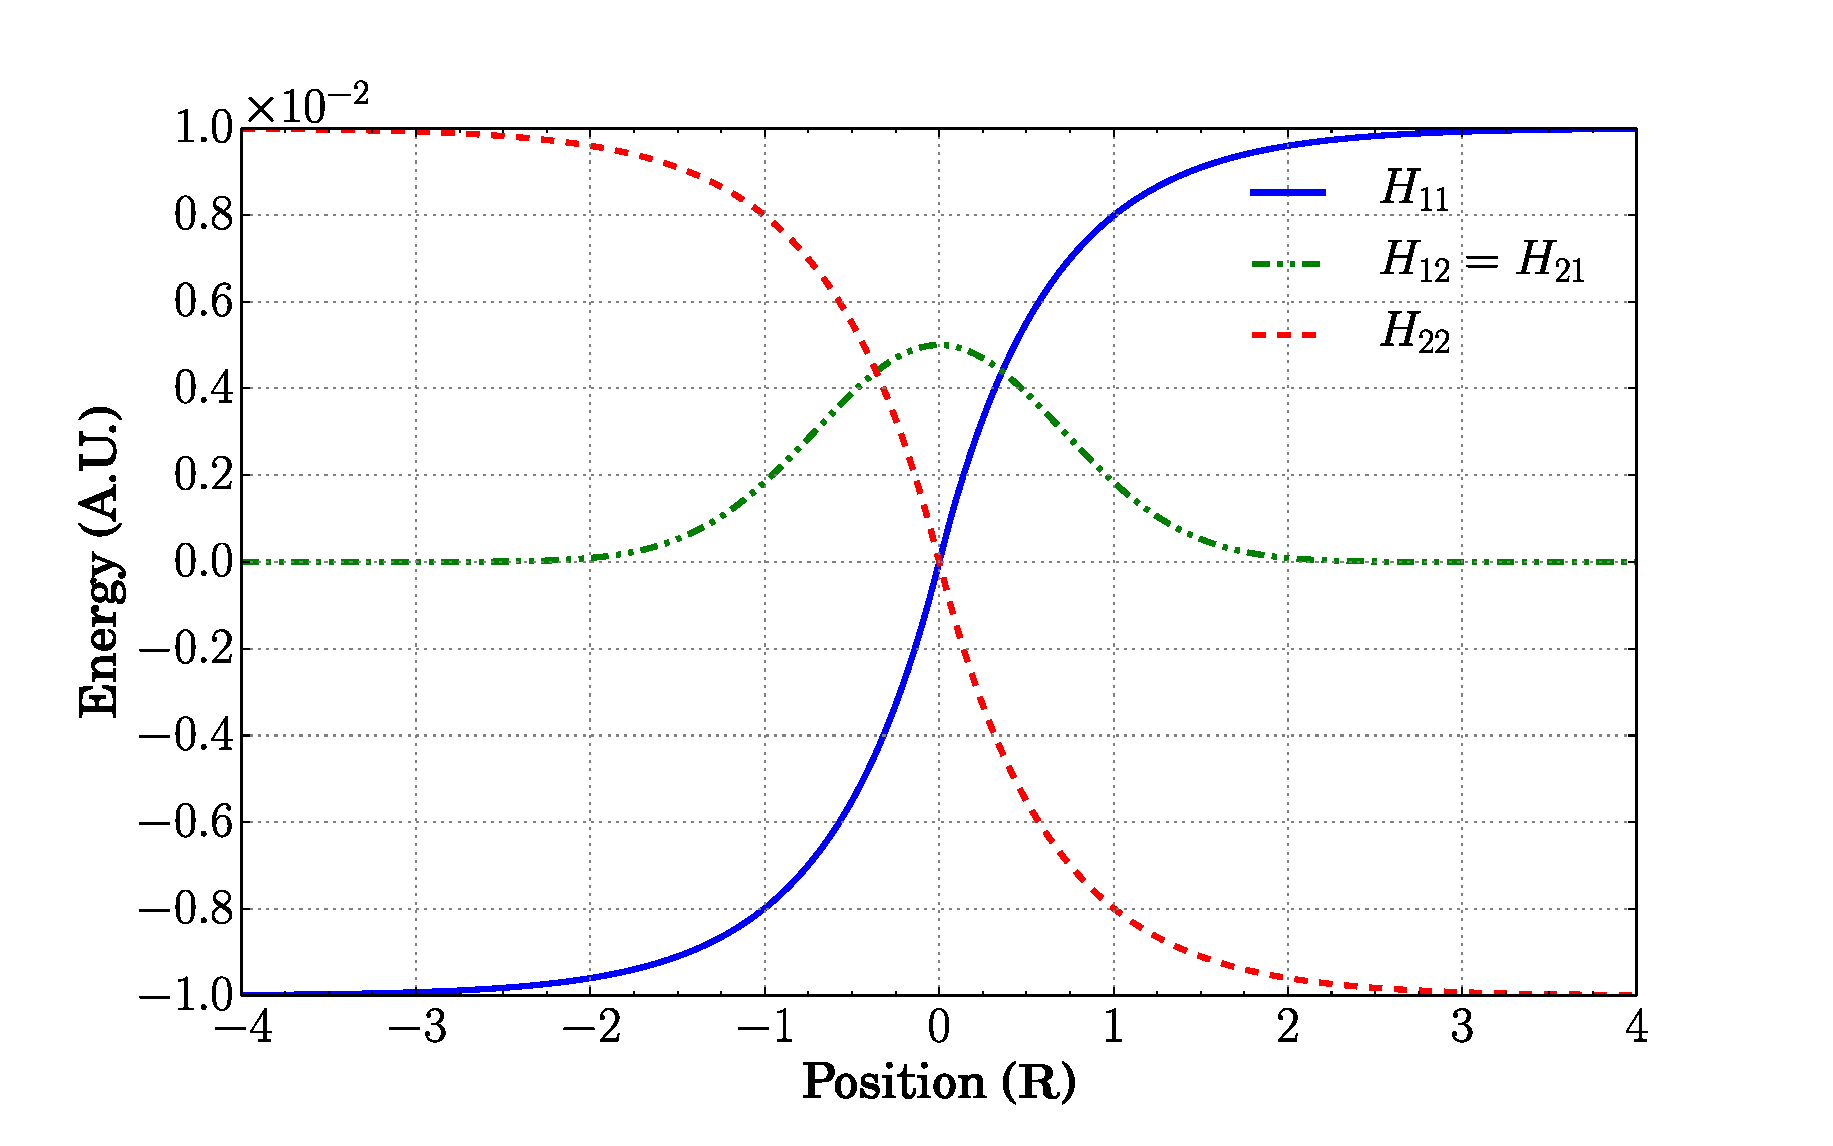
\includegraphics[width=\textwidth]{scpes.eps}
\caption[]{Diabatic PES.}
\label{sumf:pessc}
\end{subfigure}
~
\begin{subfigure}[t]{0.485\textwidth}
\centering
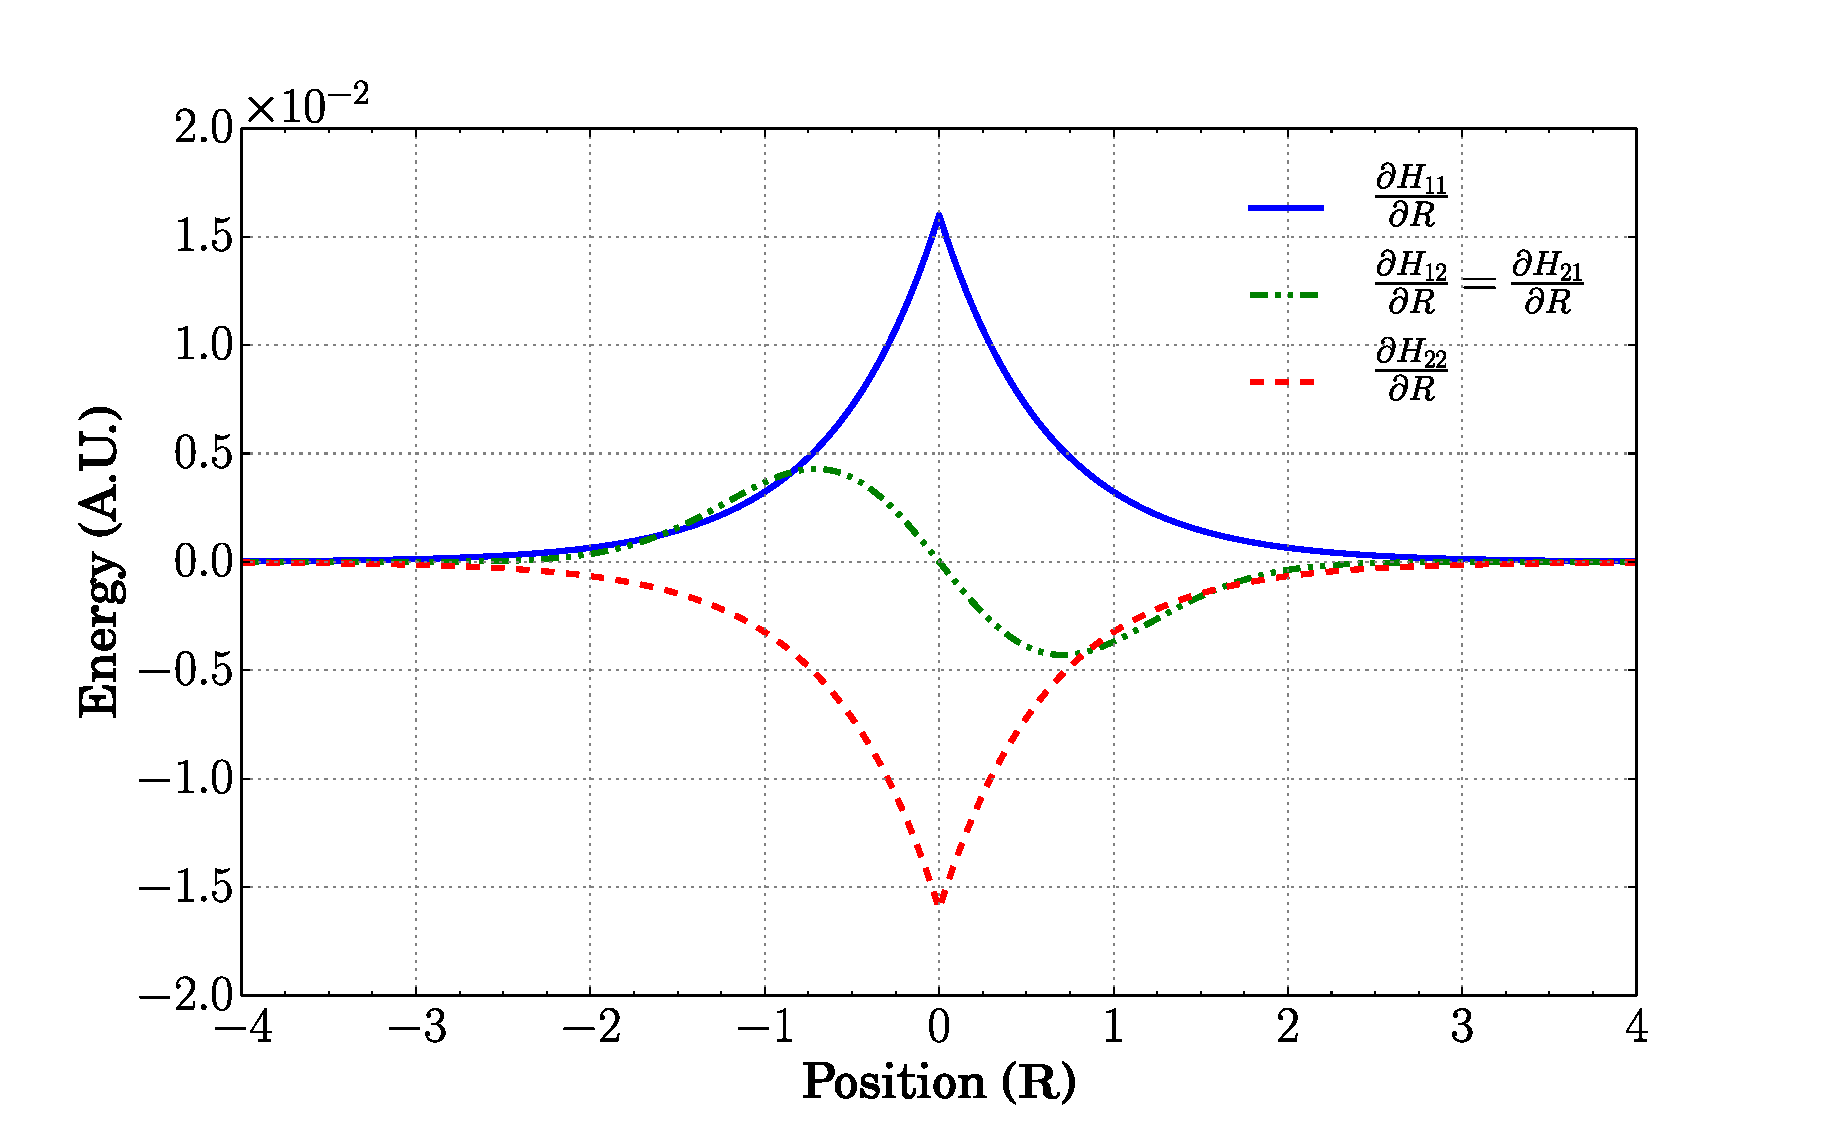
\includegraphics[width=\textwidth]{dscpes.eps}
\caption[]{Diabatic PES derivatives.}
\label{sumf:dpessc}
\end{subfigure}

\begin{subfigure}[t]{0.485\textwidth}
\centering
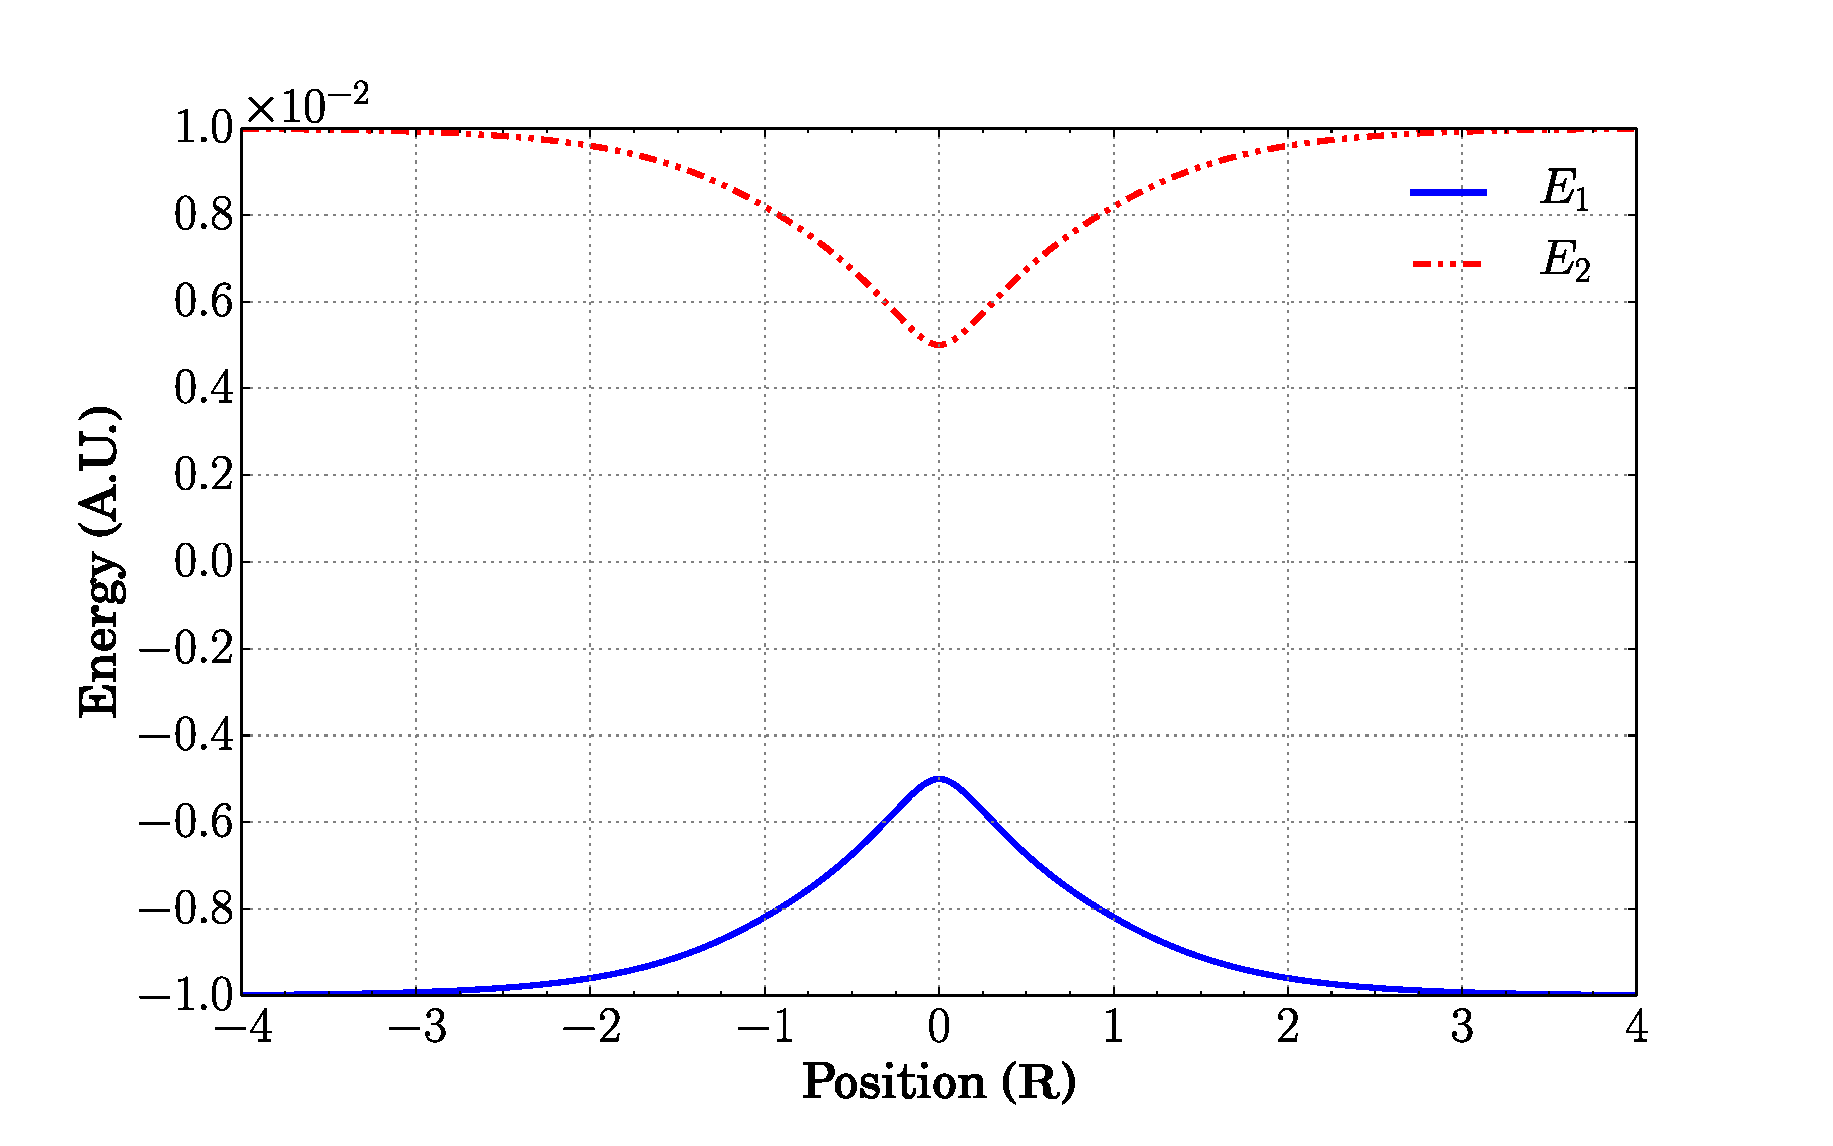
\includegraphics[width=\textwidth]{ascpes.eps}
\caption[]{Adiabatic PES.}
\label{sumf:apessc}
\end{subfigure}
~
\begin{subfigure}[t]{0.485\textwidth}
\centering
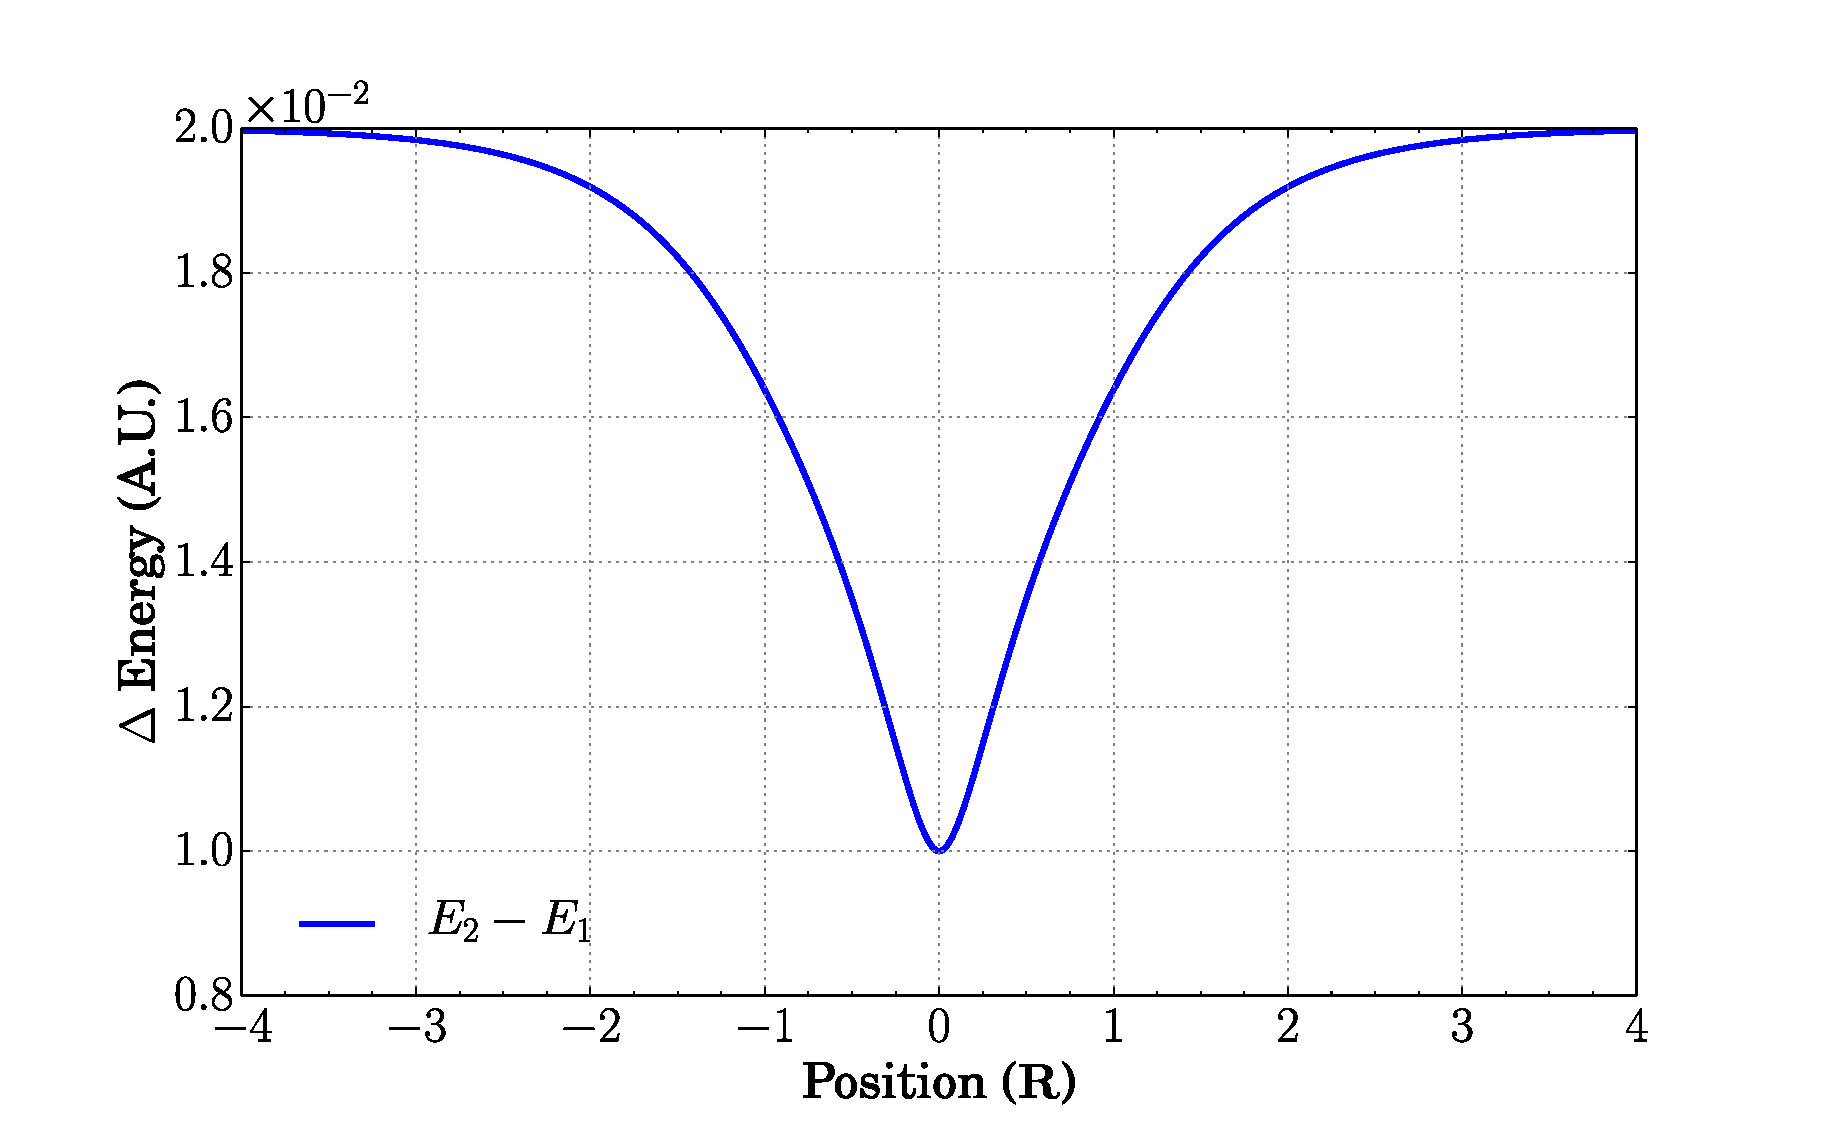
\includegraphics[width=\textwidth]{del_ascpes.eps}
\caption[]{$ \Delta E$ between adiabatic PES.}
\label{sumf:delapessc}
\end{subfigure}
\caption[]{Single avoided crossing PES.}\label{sumf:scpes}
\end{figure}
%
\subsection*{Double Avoided Crossing}
%
The diabatic potential energy surfaces (PES) for the double avoided crossing 
were defined by Tully \cite{tully} as:
\begin{subequations}
\begin{align}
H_{11}(R) &= 0 \\
H_{22}(R) &= -A e^{-B R^{2}} + E_{0}\\
H_{12}(R) &= H_{21}(R) = C e^{-D R^{2}}~,
\end{align}
\end{subequations}
where $ A = 0.1$, $B = 0.28$, $C = 0.015$, $D = 0.06$, y $E_{0} = 0.05$. The diabatic PES, their derivatives, adiabatic PES and $ \Delta E $ between adiabatic PES are plotted in \cref{sumf:dcpes}.

\begin{figure}
\centering
\begin{subfigure}[t]{0.485\textwidth}
\centering
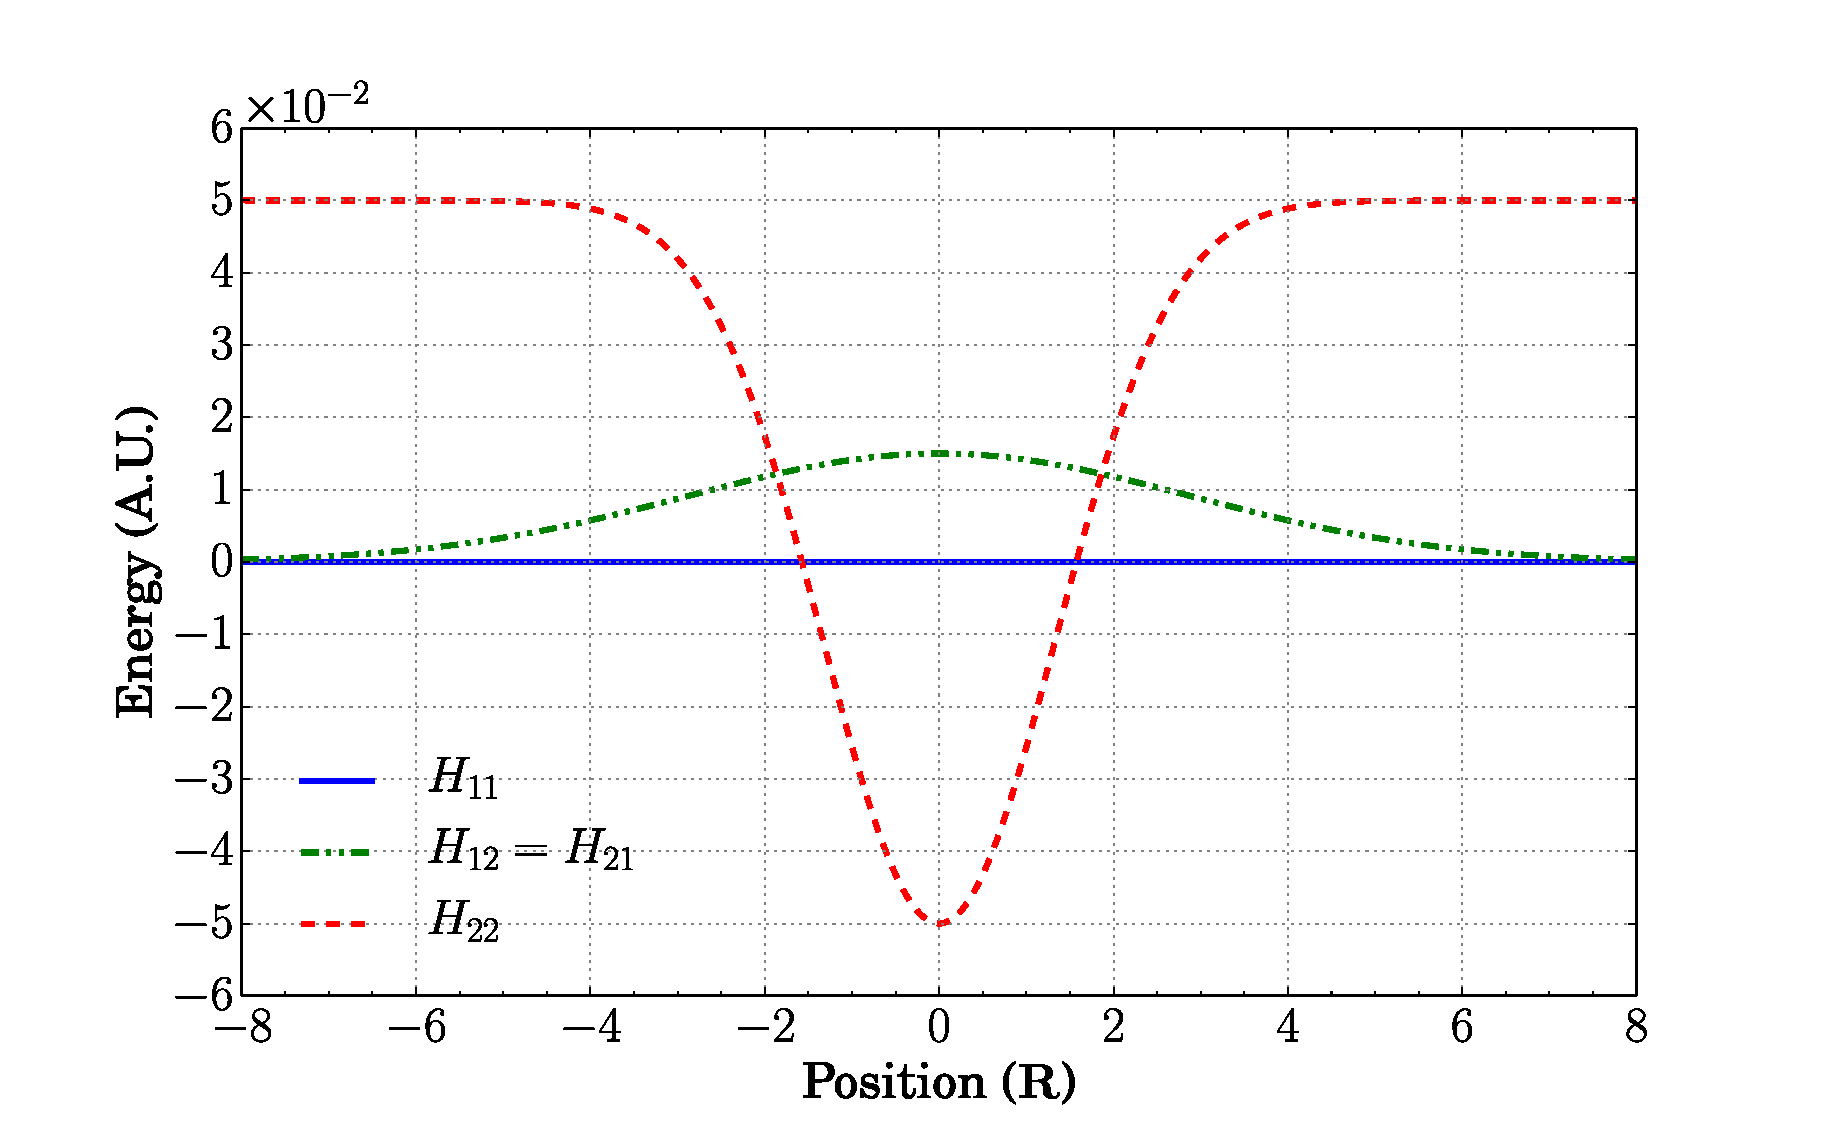
\includegraphics[width=\textwidth]{dcpes.eps}
\caption[]{Diabatic PES.}
\label{sumf:pesdc}
\end{subfigure}
~
\begin{subfigure}[t]{0.485\textwidth}
\centering
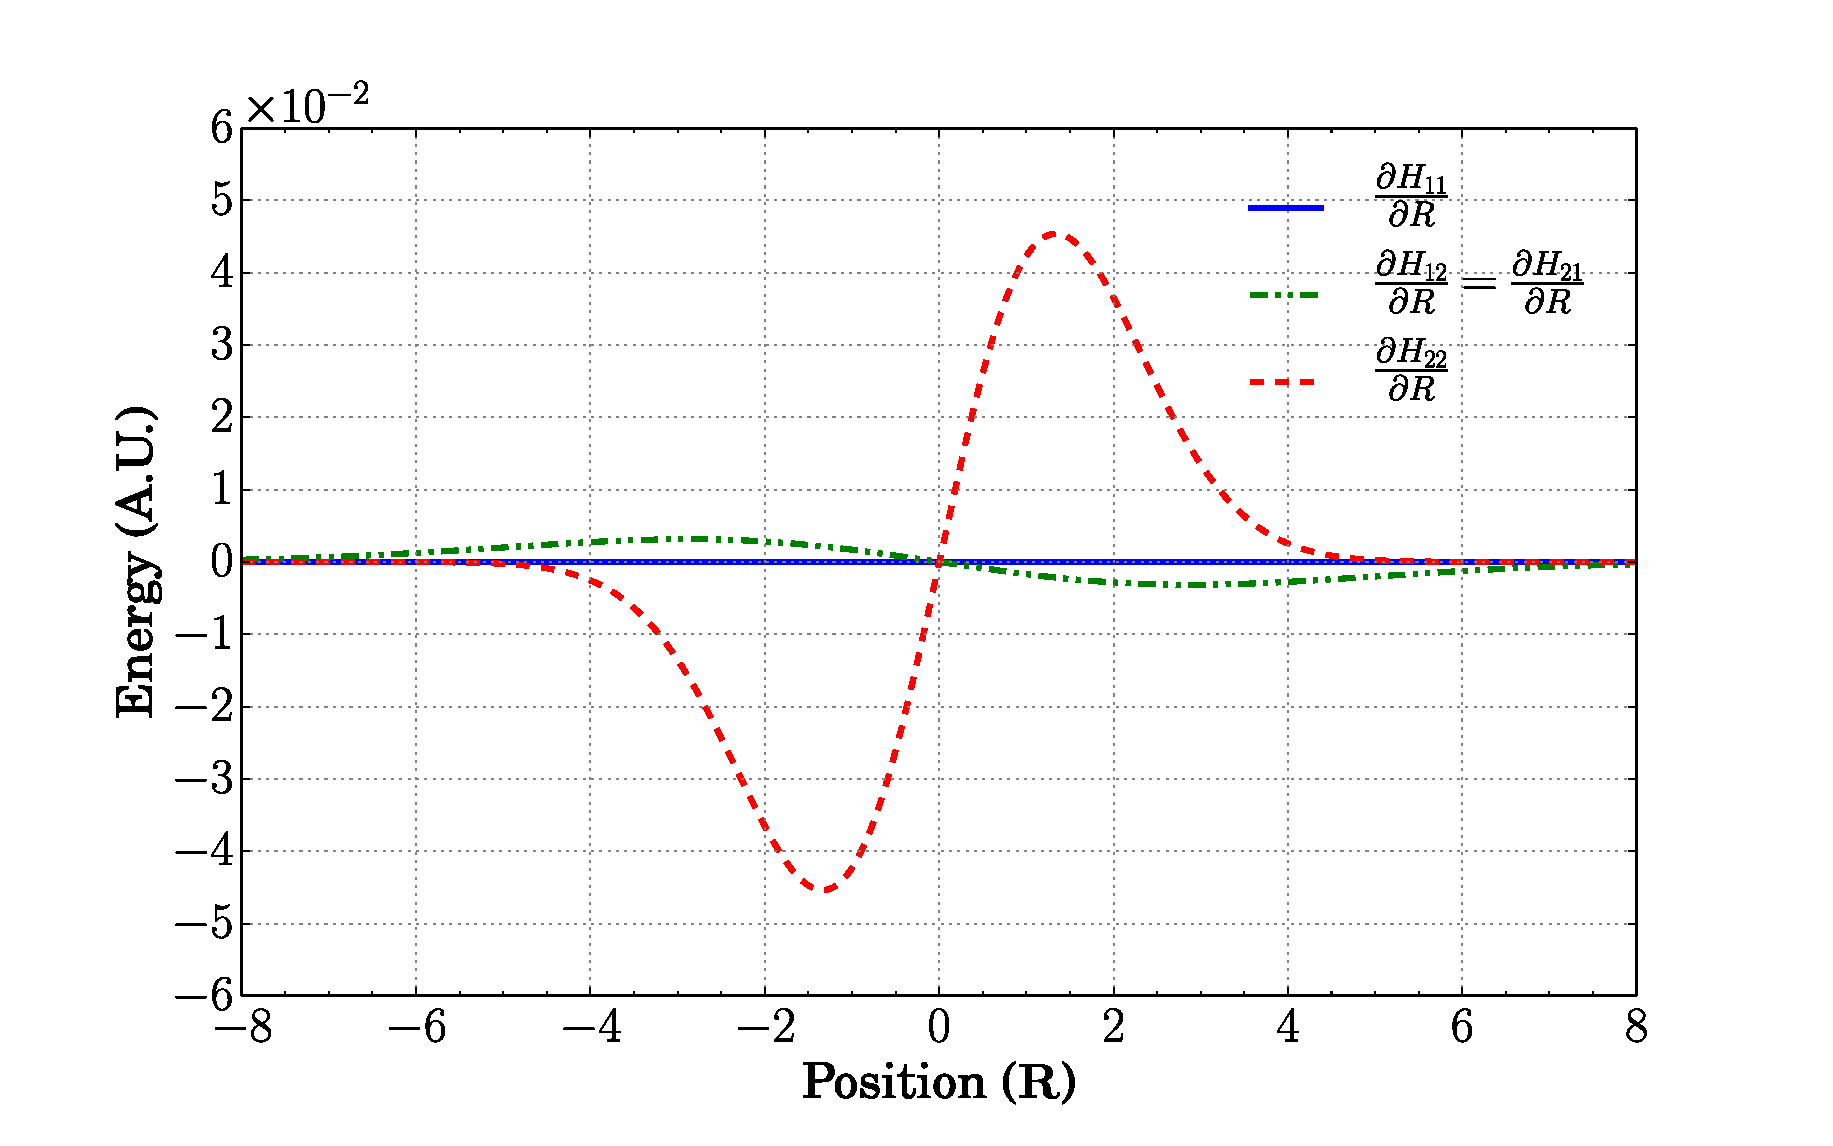
\includegraphics[width=\textwidth]{ddcpes.eps}
\caption[]{Diabatic PES Derivatives.}
\label{sumf:dpesdc}
\end{subfigure}

\begin{subfigure}[t]{0.485\textwidth}
\centering
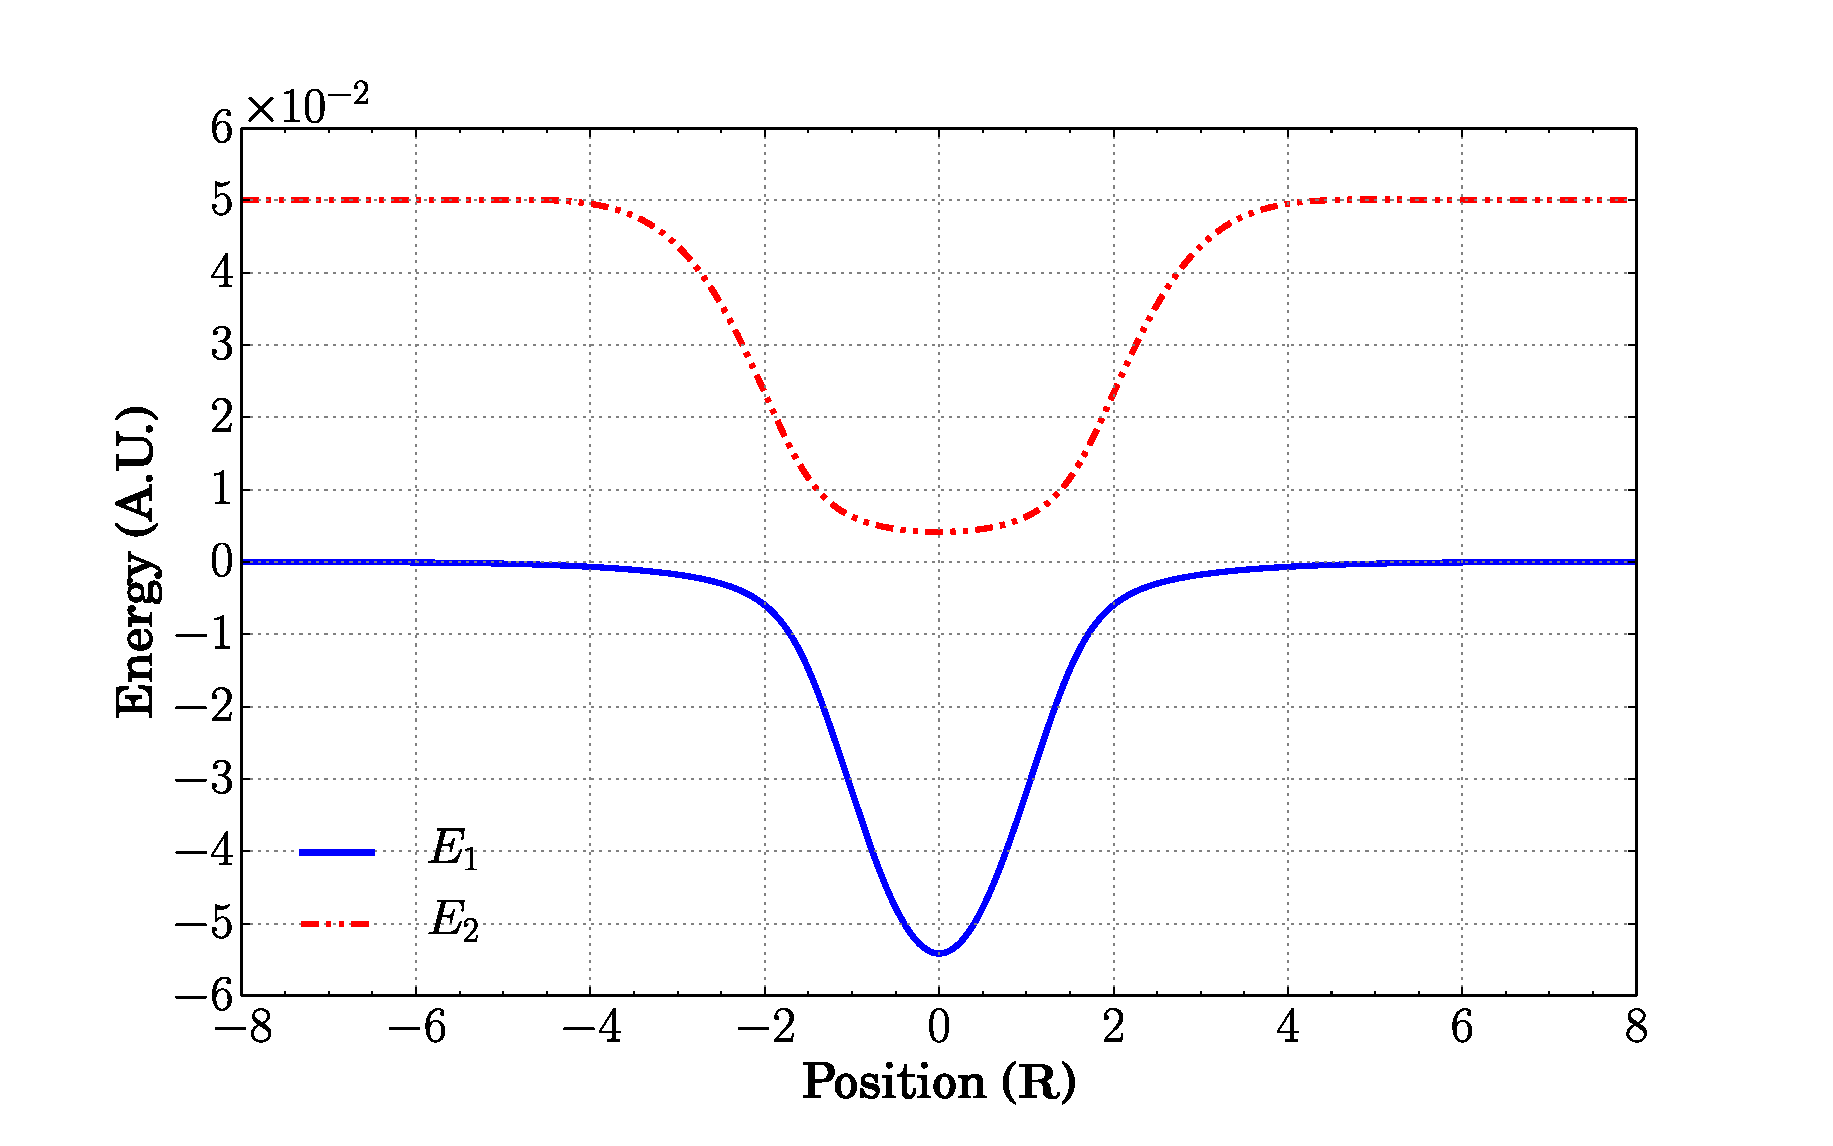
\includegraphics[width=\textwidth]{adcpes.eps}
\caption[]{Adiabatic PES.}
\label{sumf:apesdc}
\end{subfigure}
~
\begin{subfigure}[t]{0.485\textwidth}
\centering
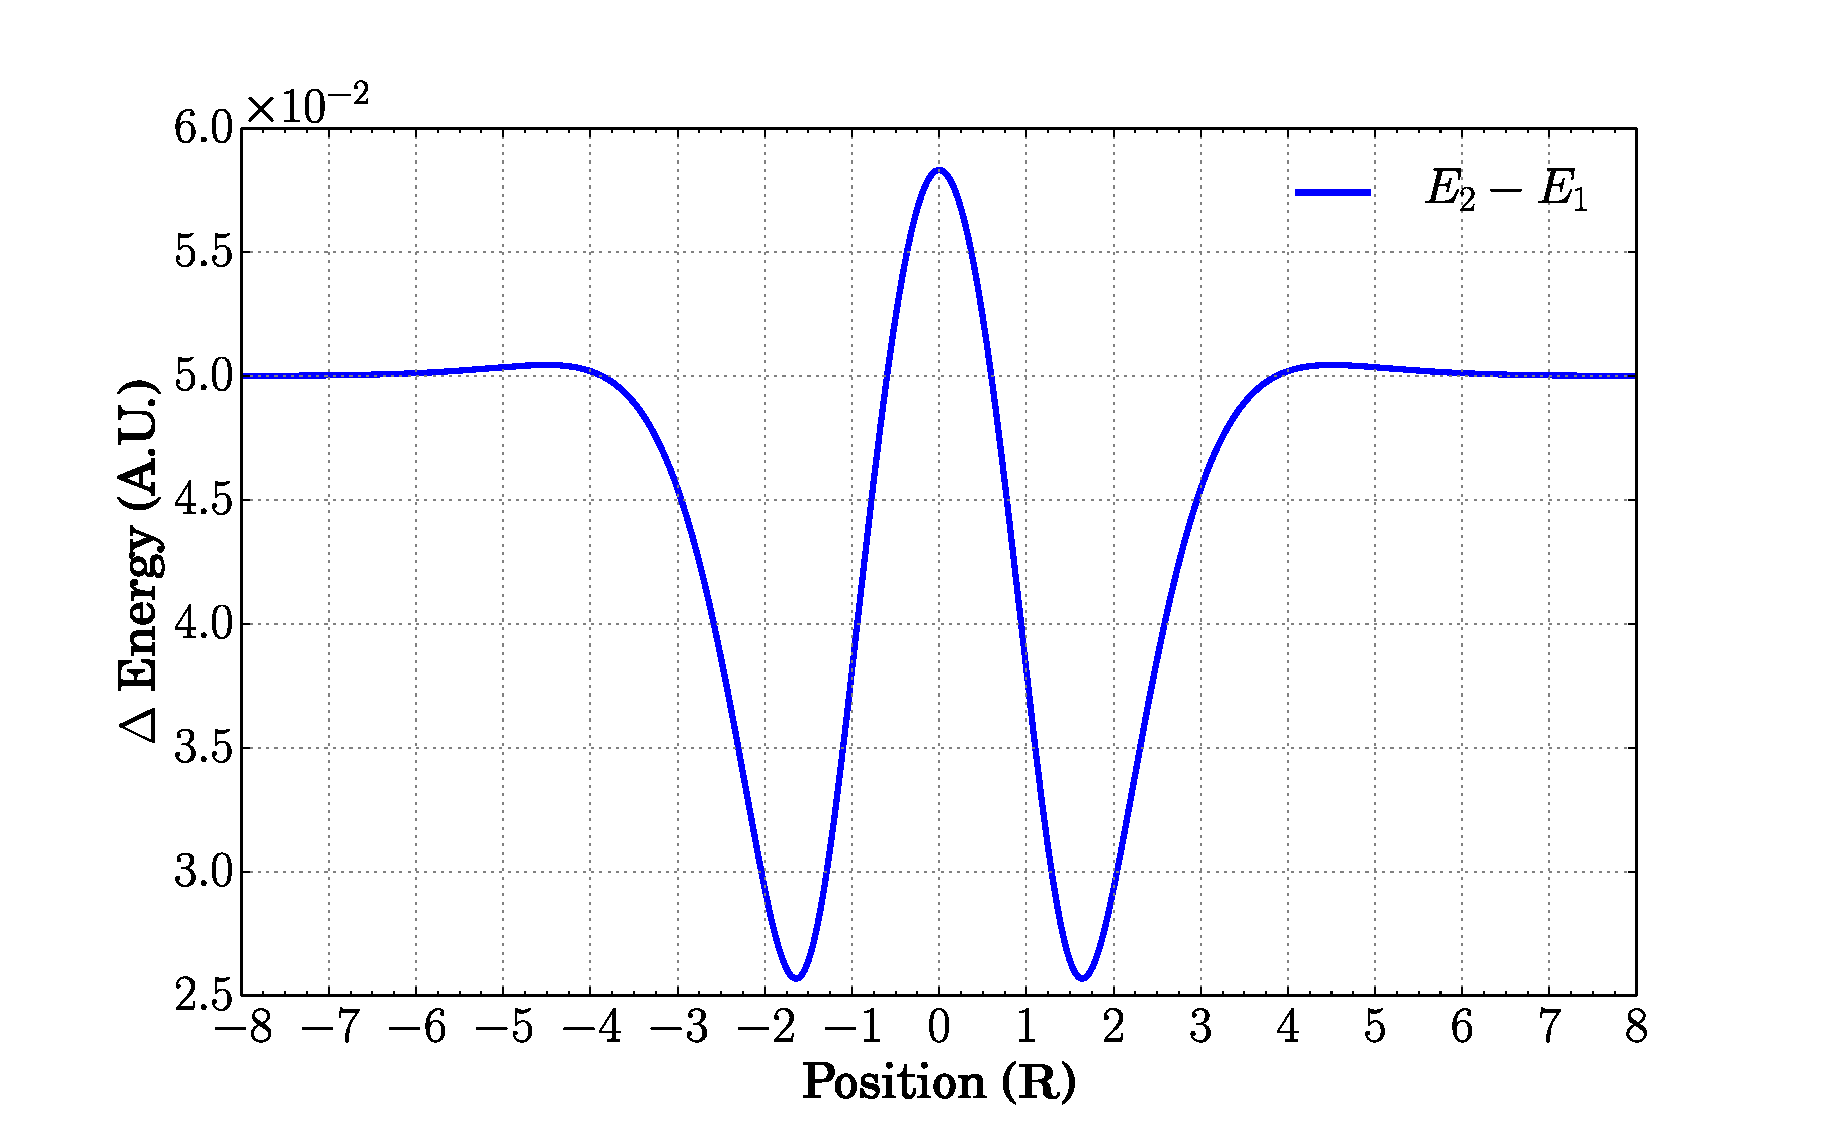
\includegraphics[width=\textwidth]{del_adcpes.eps}
\caption[]{$ \Delta E$ between adiabatic PES.}
\label{sumf:delapesdc}
\end{subfigure}
\caption[]{Double avoided crossing PES.}\label{sumf:dcpes}
\end{figure}
%
\subsection*{Extended Coupling}
%
The diabatic potential energy surfaces (PES) for the extended coupling 
were defined by Tully \cite{tully} as:
\begin{subequations}
\begin{align}
H_{11}(R) & = -A\\
H_{22}(R) & = -H_{11}\\
H_{12}(R) & = H_{21}(R) = 
\begin{cases}
B(2 - e^{-C R}) & R\geq 0 \\
B e^{C R} & R<0
\end{cases}
\end{align}
\end{subequations}
where $ A = 6 \times 10^{-4},~B = 0.1,~\text{and}~C = 0.9$. This problem has non-vanishing non-diagonal elements in the Hamiltonian matrix. Said elements are perturbations from a pure state, and when they do not vanish when $ R \rightarrow \pm\infty $, one must use the adiabatic Hamiltonian. \Cref{sumf:ecpes} shows the diabatic and adiabatic PES and their derivatives (the difference between both adiabatic PES is not shown because it's fairly obvious).

\begin{figure}
\centering
\begin{subfigure}[t]{0.485\textwidth}
\centering
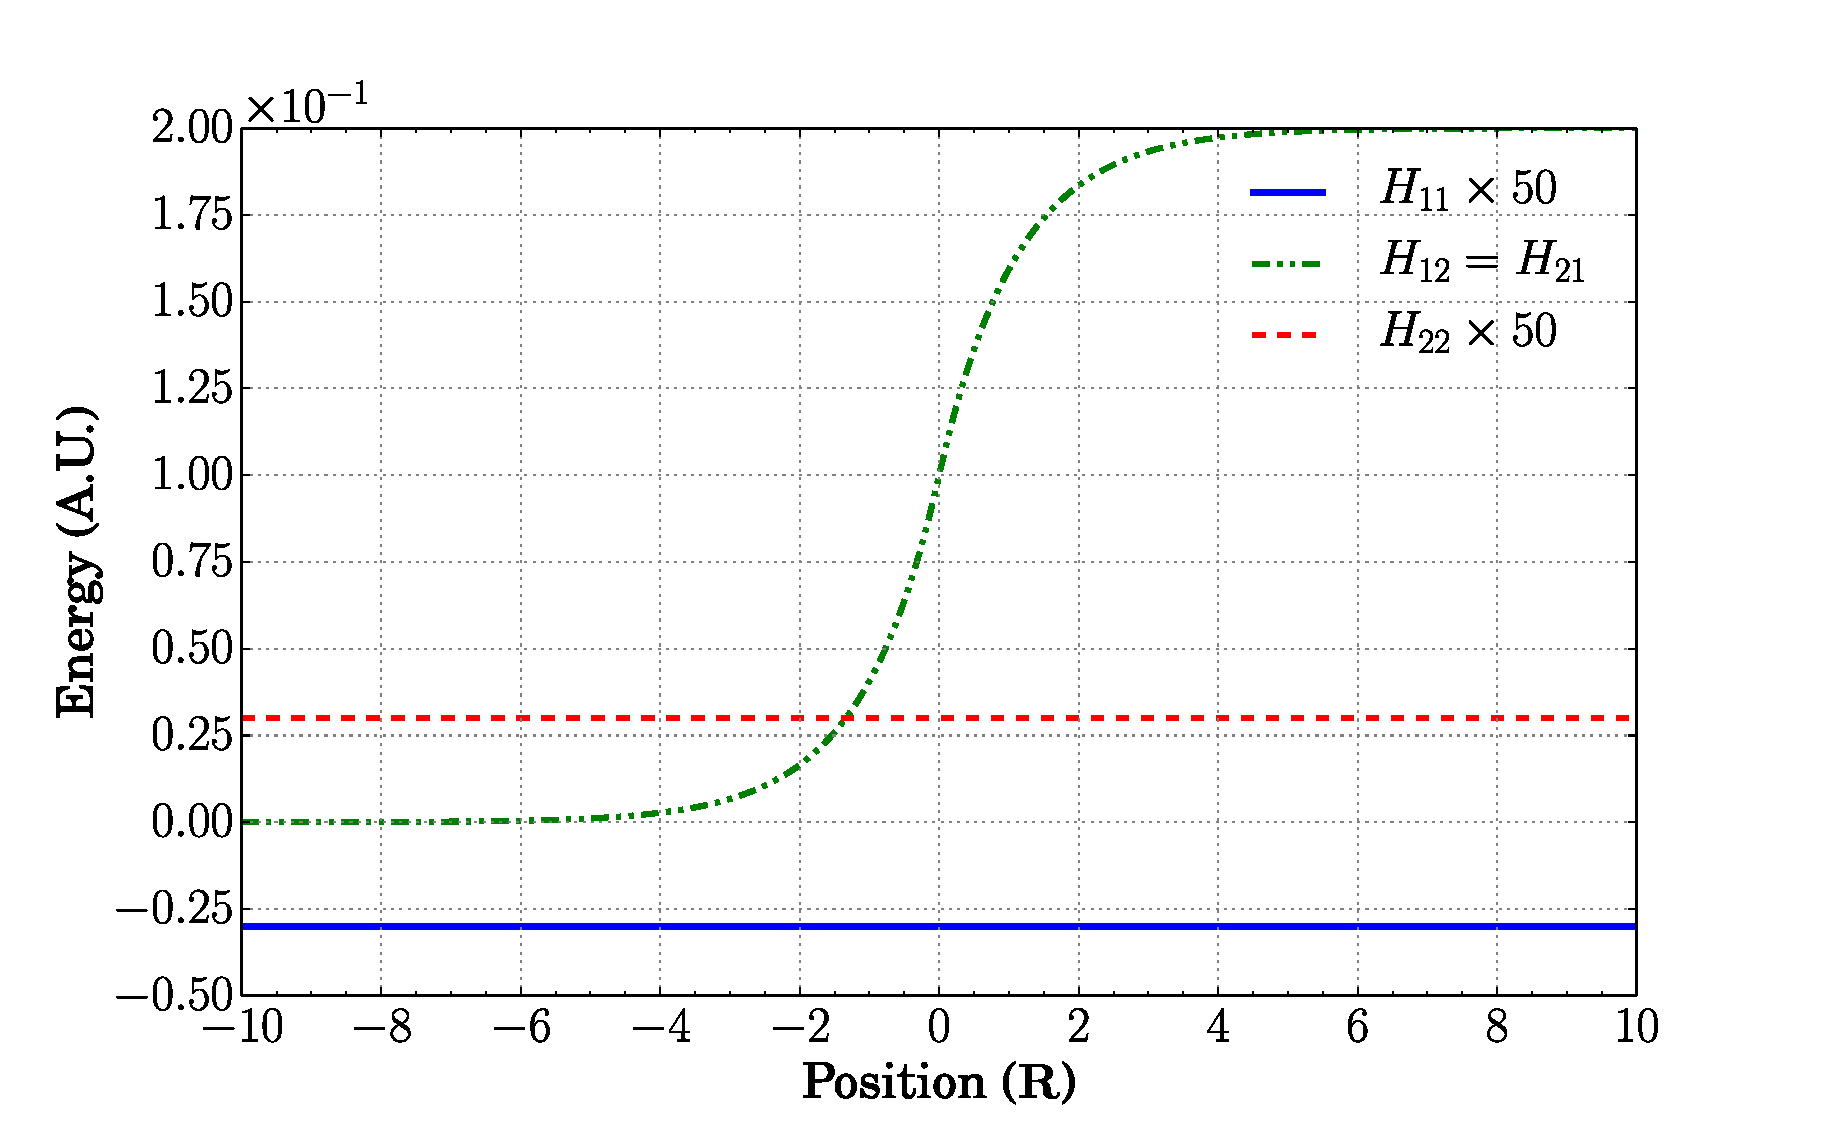
\includegraphics[width=\textwidth]{ecpes.eps}
\caption[]{Diabatic PES.}
\label{sumf:pesec}
\end{subfigure}
~
\begin{subfigure}[t]{0.485\textwidth}
\centering
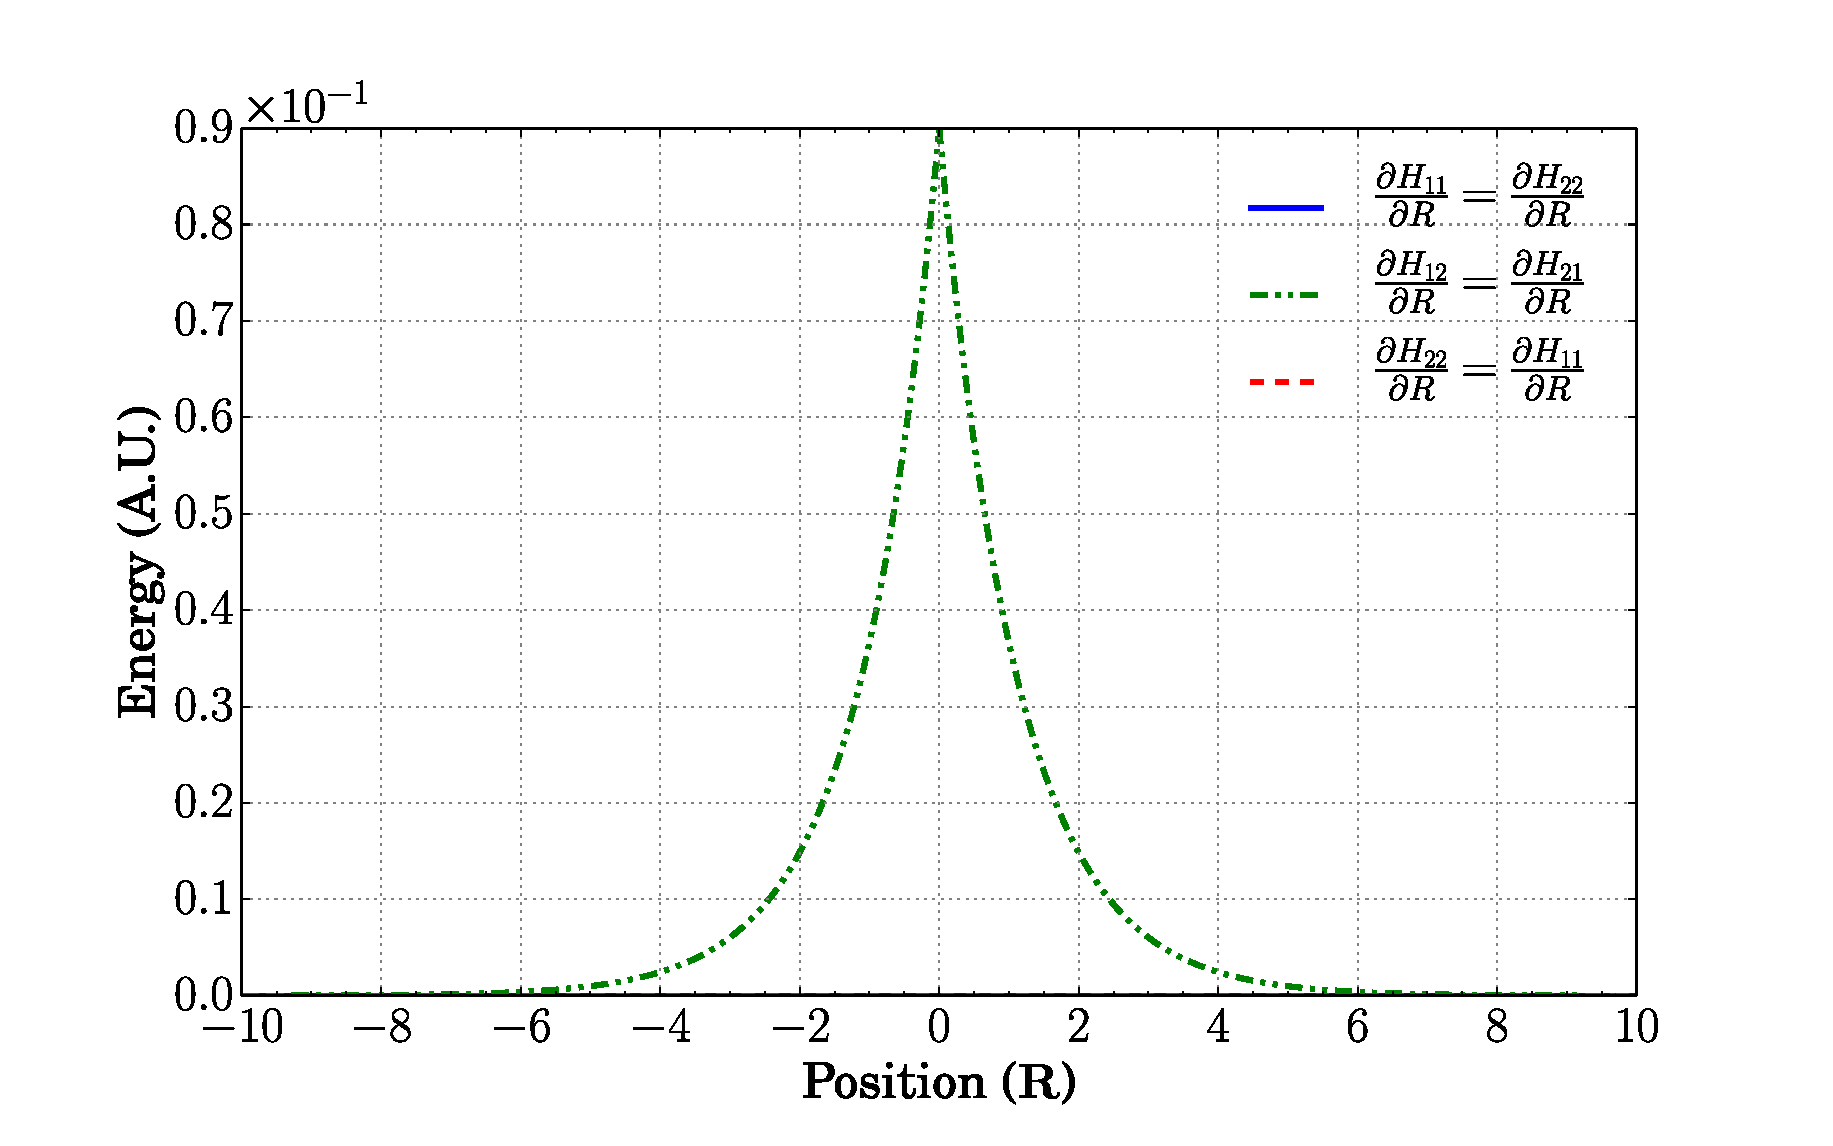
\includegraphics[width=\textwidth]{decpes.eps}
\caption[]{Diabatic PES derivatives.}
\label{sumf:dpesec}
\end{subfigure}

\begin{subfigure}[t]{0.485\textwidth}
\centering
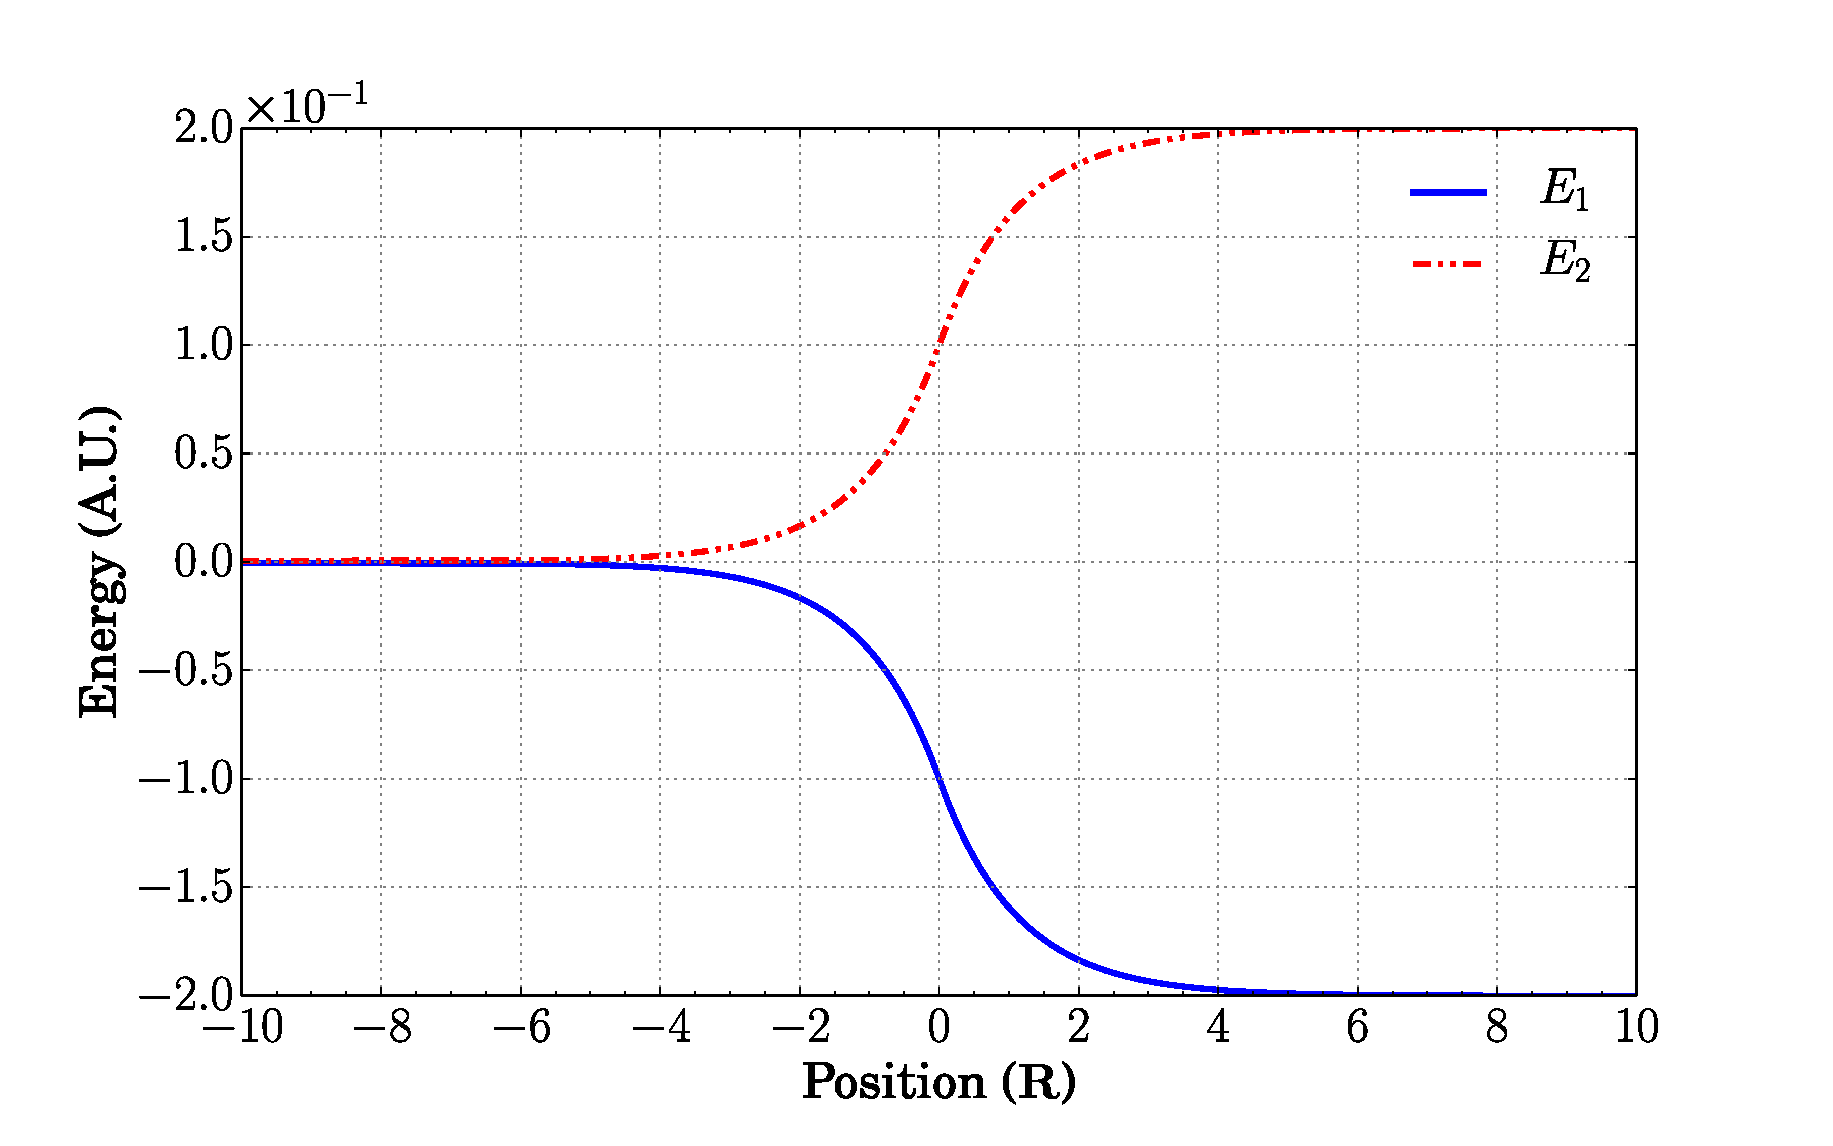
\includegraphics[width=\textwidth]{aecpes.eps}
\caption[]{Adiabatic PES.}
\label{sumf:apesec}
\end{subfigure}
~
\begin{subfigure}[t]{0.485\textwidth}
\centering
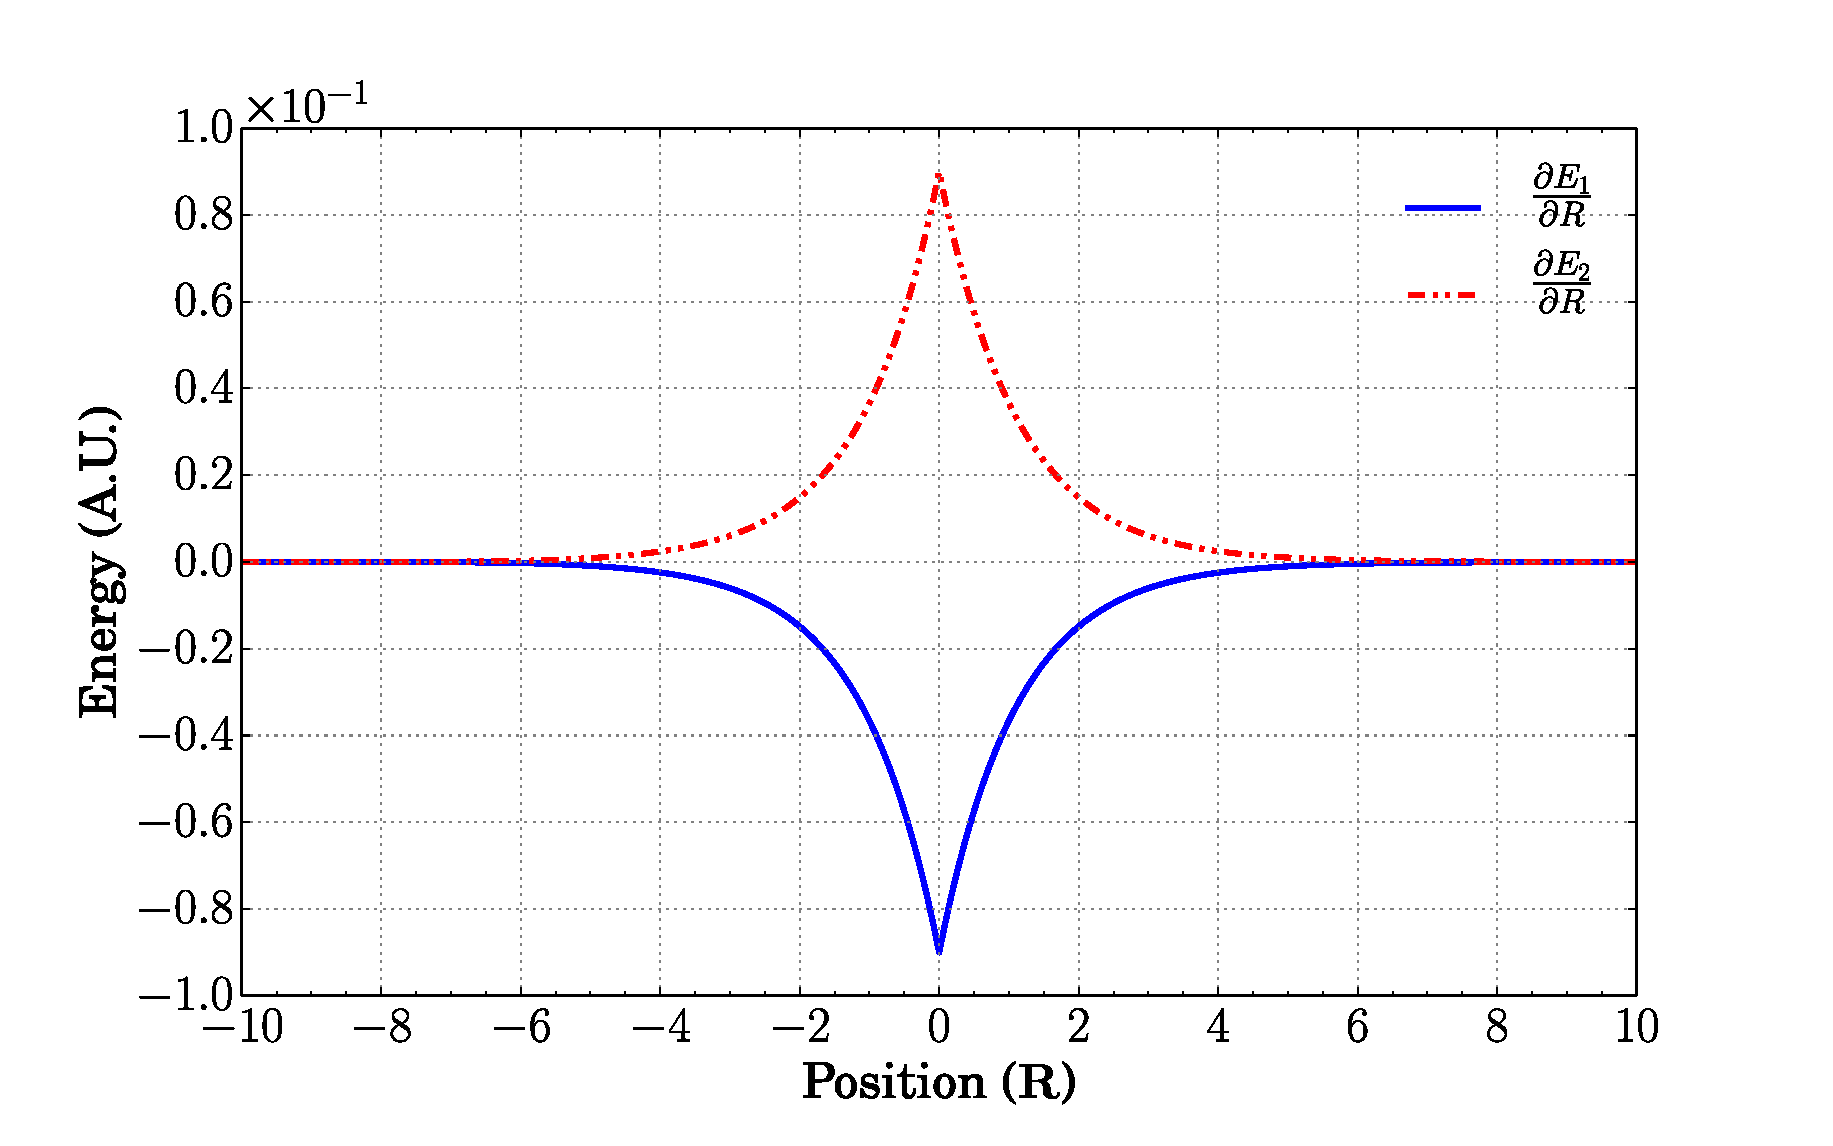
\includegraphics[width=\textwidth]{daecpes.eps}
\caption[]{Adiabatic PES derivatives.}
\label{sumf:dapesec}
\end{subfigure}
\caption[]{Extended coupling PES.}\label{sumf:ecpes}
\end{figure}
%
\subsection*{Spin-Boson Model for Condensed-Phase Dynamics}\label{sumsb:sb}
%
This problem is vastly different from the others. In our case, the model describes a 1D system of $ M $ coupled oscillators. More specifically, a one-dimensional lattice made up of $ M $ oscillating nuclei which posses bulk electronic states. What is measured here are not trajectories, but rather the time-dependent difference in the probability of finding the system in either of two electronic states; when the initial state $ =1 $, $ D(t) = P_{1\leftarrow 1} - P_{2\leftarrow 1}$, when the initial state $ =2 $, $ D(t) = P_{1\leftarrow 2} - P_{2\leftarrow 2}$.

The diabatic PES are defined as follows:
\begin{subequations}\label{e:sbpes}
\begin{align}
H_{11}(\bm{Q}) &= V_{0}(\bm{Q}) + V_{1}(\bm{Q}) + \epsilon \\
H_{22}(\bm{Q}) &= V_{0}(\bm{Q}) - V_{1}(\bm{Q}) - \epsilon \\
H_{12}(\bm{Q}) &= H_{12}(\bm{Q}) = \Delta~,
\end{align}
\end{subequations}
where,
\begin{subequations}
\begin{align}
V_{0}(\bm{Q}) &= \sum\limits_{k=1}^{M} \frac{1}{2} m_{k} \omega_{k}^{2} Q_{k}^{2} \\
V_{1}(\bm{Q}) &= \sum\limits_{k=1}^{M} c_{k} Q_{k}~.
\end{align}
\end{subequations}
For our purposes, the frequencies, $ \omega_{k} $, are uniformly distributed $ \in [0.01 \omega_{c},~4 \omega_{c}] $ \cite{spin-boson}, where $ \omega_{c} $ is known as the \emph{characteristic frequency}, and defines the system's overall time scale. The observant reader will realise this does not make a lot of sense on its own, because not all frequencies contribute to a system's energy in equal amounts. Which is why the coupling parameters, $ c_{k} $, are chosen so they obey the distribution:
\begin{align}\label{e:sb_dd}
J(\omega) = \frac{\pi}{2} \sum\limits_{k=1}^{M} \frac{c_{k}^{2}}{m_{k} \omega_{k}}  \delta(\omega - \omega_{k})~,
\end{align}
where $ J(\omega) $ is an Ohmic distribution defined as:
\begin{align}\label{e:sb_cd}
J(\omega) = \frac{\pi}{2} \alpha \omega \exp\left(-\frac{\omega}{\omega_{c}}\right)~,
\end{align}
where $ \alpha $ is the Kondo parameter (a coupling strength parameter). After equating \cref{e:sb_dd,e:sb_cd}, and integrating with respect to $ \omega $, we find the values of $ c_{k} $ to be:
\begin{subequations}
\begin{align}
c_{k} & = \sqrt{\frac{2}{\pi} \Delta \omega m_{k} \omega_{k} J(\omega_{k})}
= \omega_{k} \sqrt{\alpha \Delta \omega m_{k} \exp\left(-\frac{\omega_{k}}{\omega_{c}}\right)} \\
\Delta \omega &= \frac{\omega_{max} - \omega_{min}}{M - 1}~.
\end{align}
\end{subequations}

The initial electronic conditions are initiated in the same manner as before. However, the nuclear ones are not. As stated before, the model describes oscillating nuclei in a 1D lattice, and their momenta and positions are assumed to follow the Wigner distribution:
\begin{subequations}
\begin{align}
\rho(\bm{P},\bm{Q}) &= \prod\limits_{k=1}^{M} \exp\left(-a_{k} \frac{P_{k}^{2}}{2 m_{k}}\right)\cdot
\exp\left(-a_{k} \frac{1}{2} m_{k} \omega_{k}^{2} \left[Q_{k} + \frac{c_{k}}{m_{k} \omega_{k}^{2}}\right]^{2} \right)\\
a_{k} &= \frac{2}{\omega_{k}} \tanh\left(\frac{\beta \omega_{k}}{2}\right)~.
\end{align}
\end{subequations}
Which, in reality, is a bivariate normal distribution. Fortunately, the lack of a covariant term implies that positions and momenta can be independently sampled from normally distributed random numbers. In other words, the nuclei follow independent normal distributions for their momenta and positions. It is also worth noting that the argument for the total distribution is basically a scaled quasiclassical analogue of the quantum harmonic oscillator Hamiltonian operator ($ \hat{H} = \frac{\hat{p}^{2}}{2m} + \frac{1}{2} m \omega^{2} \hat{x}^{2}$), which makes a lot of intuitive sense, because it means the nuclear parameters are sampled according to the oscillators' normally distributed kinetic energy.

Sampling is done in the traditional way: assuming $ X $ is a normally distributed random number with unitary standard deviation and mean equal to zero, a normally distributed random number $ G $ with standard deviation equal to $ \sigma $ and mean equal to $ \mu $ can be calculated by $ G = \sigma X + \mu $. Given the definition of the normal distribution,
\begin{align}
G(x, \mu, \sigma) = \frac{1}{\sigma \sqrt{2\pi}} \exp\left(- \frac{(x-\mu)^{2}}{2 \sigma^{2}}\right),
\end{align}
the standard deviations and mean values of the nuclei's momenta and positions are:
\begin{subequations}
\begin{align}
&\sigma_{P_{k}} = \sqrt{\frac{m_{k} \omega_{k}}{2 \tanh\left(\frac{\beta \omega_{k}}{2}\right)}}\\
&\mu_{P_{k}} = 0\\
&\sigma_{Q_{k}} = \sqrt{\frac{1}{2 m_{k} \omega_{k} \tanh\left(\frac{\beta \omega_{k}}{2}\right)}}\\
&\mu_{Q_{k}} = -\frac{c_{k}}{m_{k} \omega_{k}^{2}}~.
\end{align}
\end{subequations}
%
\section*{Results}
%
The code written to implement the model was found to scale linearly with integration step, number of MC repetitions and number of cores used. It was also found that accuracy is more dependent on the number of MC repetitions than the size of the integration step, $ h $. In fact, the integration step could be made relatively large (how large depends on the problem) without significantly affecting accuracy, but drastically reducing computational time. There was also no significant difference between using $ \gamma = \frac{\sqrt{3}-1}{2} $ and $ \gamma = 0.366 $ (the actual value is very similar, but there is no need to evaluate square roots and divisions all the time if we use the approximation); \cite{project} gives the theoretical justification for this value, but it can be adjusted on a case by case basis. Accuracy was also not noticeably affected by parallel runs, presumably due to the random number generator used---which is thread safe---but not optimal for parallelisation, because it generates numbers in sequence from a single source rather than in parallel\footnote{See \url{https://gcc.gnu.org/onlinedocs/gfortran/RANDOM_005fNUMBER.html}} (it only affects execution speed).

The number of MC repetitions (MC reps) $ = 15000 $ and the value of $ \gamma = 0.366 $ unless stated otherwise. Reflections are denoted as $ R $ and transmissions as $ T $, electronic transitions from an initial state, $ i $, to a final state, $ f $, are denoted as $ f \leftarrow i $.
%
\subsection*{Single Avoided Crossing}
%
\begin{figure}
\begin{subfigure}[t]{0.5\textwidth}
\centering
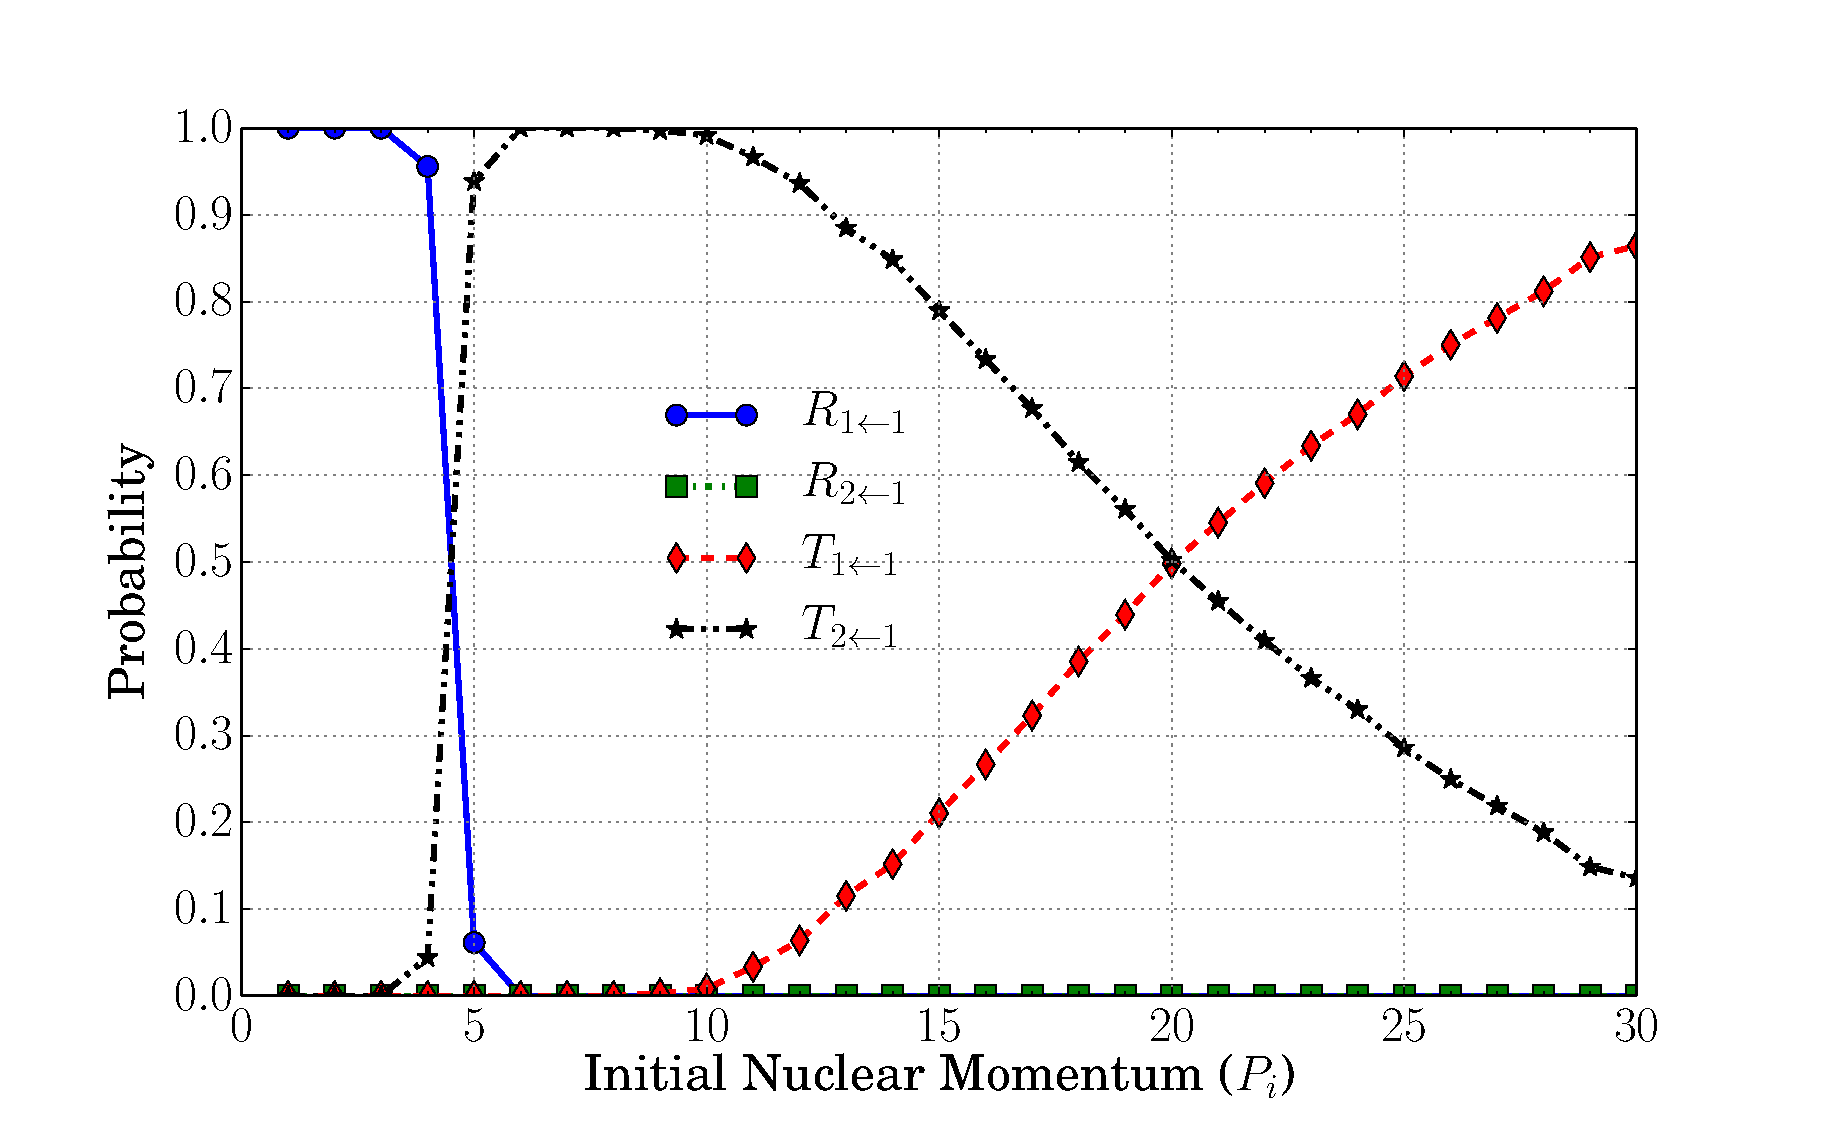
\includegraphics[width=\textwidth]{sc_prob_lh.eps}
\caption[]{Transition probabilities for Reflection ($ R $) and Transmission ($ T $) for $ h = (0.012P_{i})^{-1} $ and initial state $ = 1 $.}
\label{sumf:sci1}
\end{subfigure}
~
\begin{subfigure}[t]{0.5\textwidth}
\centering
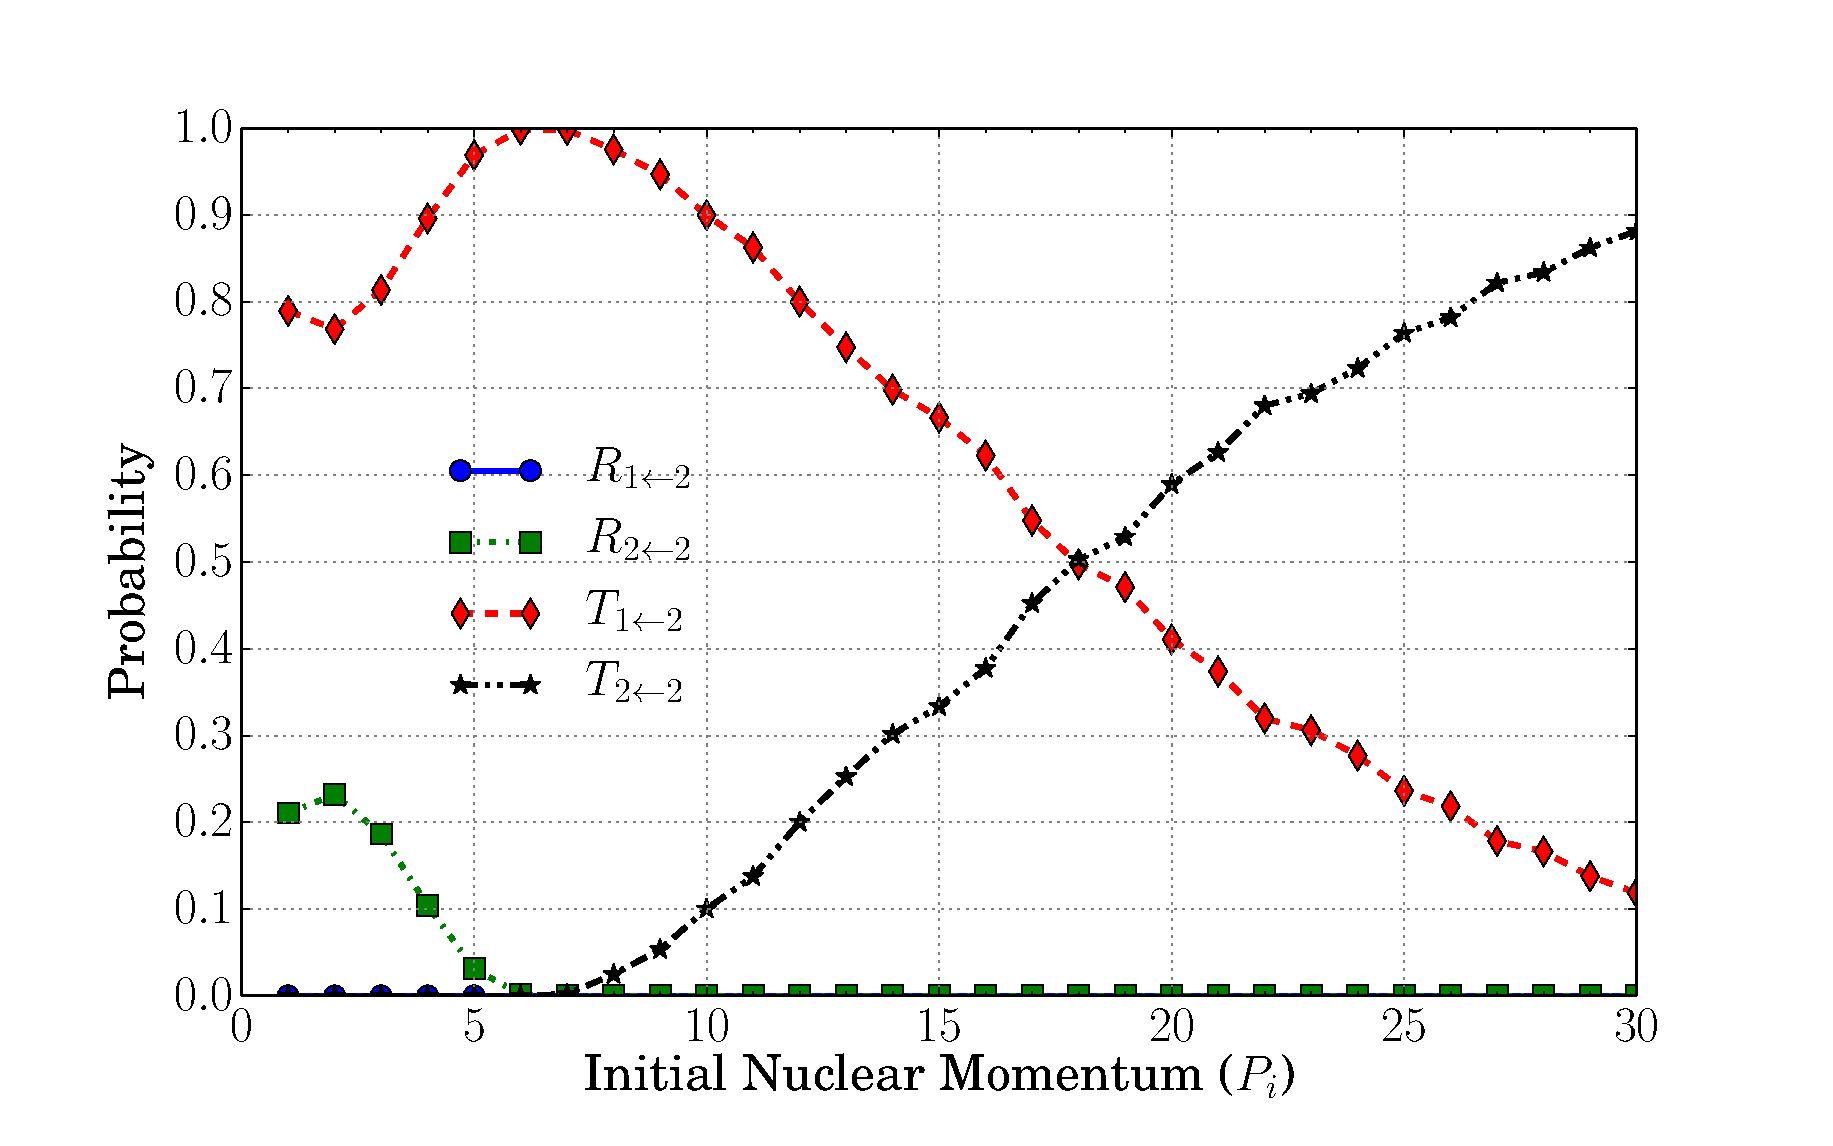
\includegraphics[width=\textwidth]{sc_prob_i2.eps}
\caption[]{Transition probabilities for Reflection ($ R $) and Transmission ($ T $) for $ h = (0.012P_{i})^{-1} $ and initial state $ = 2 $.}
\label{sumf:sci2}
\end{subfigure}
\caption[]{Single avoided crossing transition probabilities.}\label{sumf:sc}
\end{figure}

The results for when initial state $ = 1 $ are very similar---though not exactly the same---as those found in \cite{project}. However, this is most likely down to the fact that they used $ 50000\text{--}100000$ trajectories as well as there being a strong possibility that the compiler, RNG, and integration step differ. \Cref{sumf:sc} showcases the results for initial state $ = 1, 2 $.

Despite this being the simplest problem tackled herein, it presents some fairly interesting behaviours.

First, we shall tackle \cref{sumf:sci1}. The behaviour of \roo---whose probability is seen to rapidly decline as nuclear momentum increases---can be explained by referring back to \cref{sumf:scpes}. For small values of nuclear momentum, there is not enough kinetic energy to scale over the potential barrier (akin to an `activation energy') and continue in the original direction, thus the particle is reflected back. The behaviour of \rto~is explained by the same reason; once there is enough kinetic energy to reach a point where a transition is likely to happen, there would also be enough energy to continue on to the other side. Thus \rto~remains relatively close to zero throughout. The others can be explained by the fact that transition probabilities are not only a function of the distance between adiabatic PES, but also on the time it takes the particle to move away from the areas where this value is small. This explains why the \tto~and \too~transitions behave the way they do. In the case of \tto~lower nuclear momenta allow more time for an electronic transition to occur; however, after a certain value of nuclear momentum, it begins to decrease in favour of \too~because time the particle travels so fast that it cannot interact long enough to undergo an electronic transition.

For \cref{sumf:sci2} the behaviour is more nuanced, but down to mostly the same reasons. The \rot~transition remains effectively zero throughout because at such low values of nuclear momenta two things can happen: the particle can't get past the dip in $ E_{2} $ (if it doesn't move to the lower energy state) because it gets reflected back by the off-diagonal PES---corresponding to the \rtt~transition---or it moves down to the lower energy state, where the surplus potential energy is converted into kinetic energy (conservation of energy) and a \tot~transition is observed. For higher values of nuclear momentum, the particle has enough energy to be transmitted, but there is not enough time for the particle to linger long enough for there to be a state transition, and \ttt~is observed instead, and the higher the nuclear momentum the less time there is and the likelier said process becomes.
%
\subsection*{Double Avoided Crossing}
%
\begin{figure}
\begin{subfigure}[t]{0.5\textwidth}
\centering
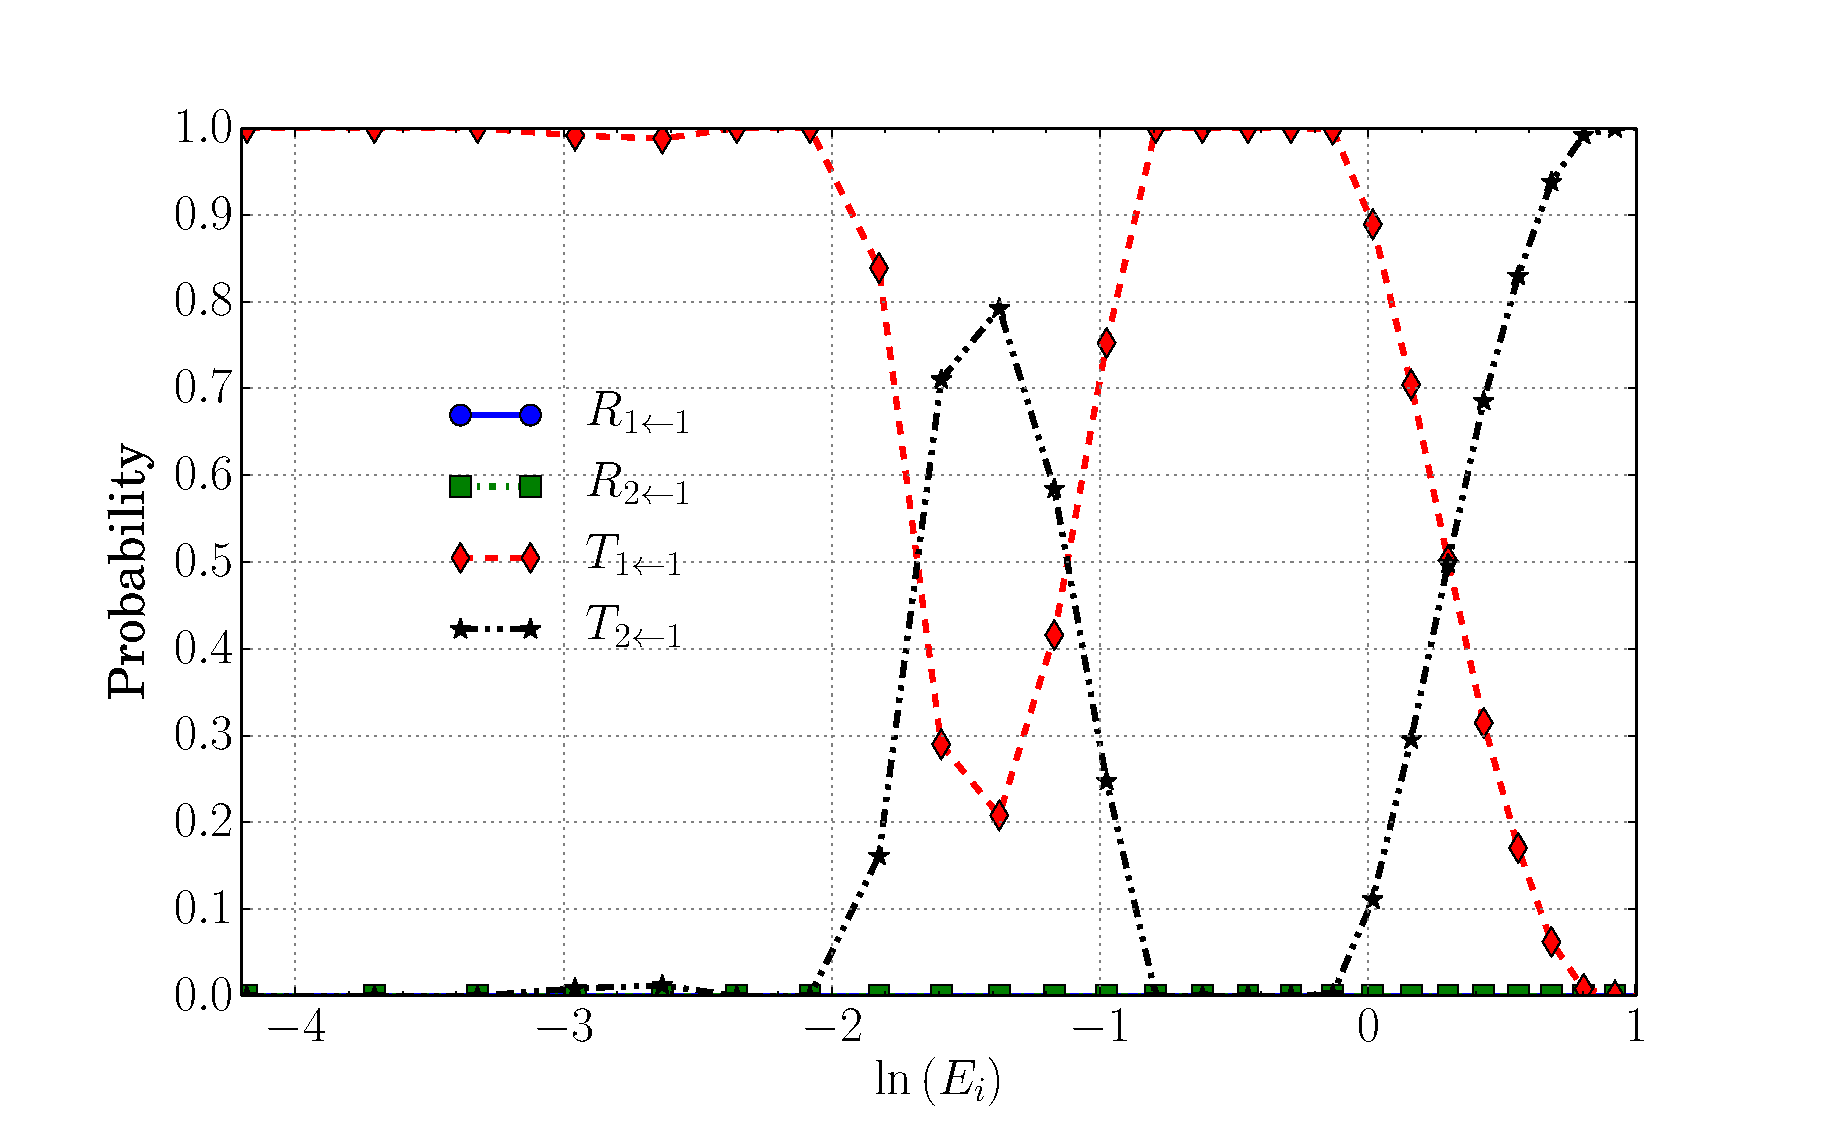
\includegraphics[width=\textwidth]{dc_prob_lh.eps}
\caption[]{Transition probabilities for Reflection ($ R $) and Transmission ($ T $) for $ h = (0.0125P_{i})^{-1} $ and initial state $ = 1 $.}
\label{sumf:dci1}
\end{subfigure}
~
\begin{subfigure}[t]{0.5\textwidth}
\centering
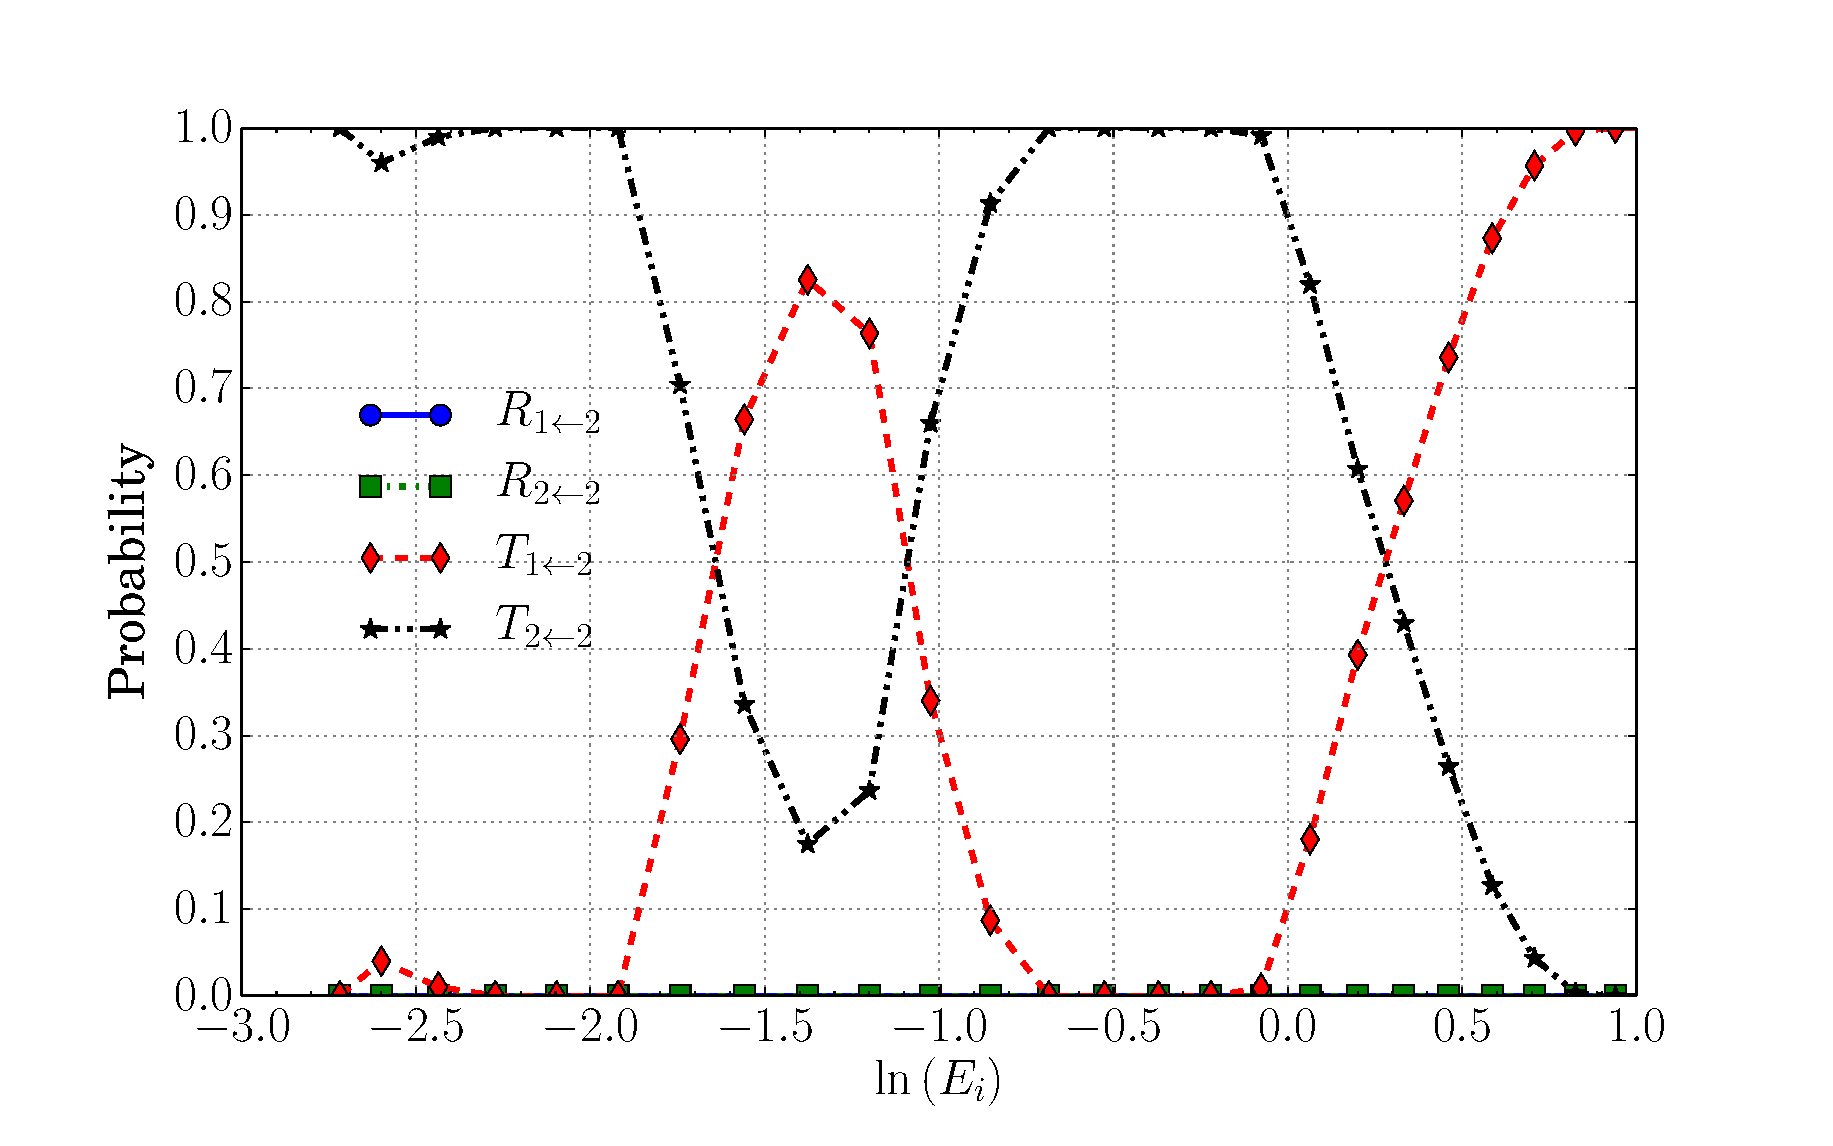
\includegraphics[width=\textwidth]{dc_prob_i2.eps}
\caption[]{Transition probabilities for Reflection ($ R $) and Transmission ($ T $) for $ h = (0.0125P_{i})^{-1} $ and initial state $ = 2 $.}
\label{sumf:dci2}
\end{subfigure}
\caption[]{Double avoided crossing transition probabilities.}\label{sumf:dc}
\end{figure}

Again the results for when initial state $ = 1 $ are very similar---but not exactly the same---as those found in \cite{project}. Which can be attributed to the same factors as before. \Cref{sumf:dc} shows the results for initial state $ = 1, 2 $.

Once more, we shall first analyse the behaviour for initial state $ = 1 $, shown in \cref{sumf:dci1}. The lack of \roo~and \rto~transitions is easily explained by the fact there is no energy barrier in either the diagonal diabatic or adiabatic PES (\cref{sumf:pesdc,sumf:apesdc}), therefore the particle only requires a small amount of momentum for the particle to be transmitted. In fact, in low momentum tests, the particle was accelerated by the adiabatic energy wells (potential energy was transferred into kinetic energy). The more interesting features are the Stückelberg oscillations for both \too~and \tto, which are often attributed to quantum interference effects. In order to comprehend these one must only turn to \cref{sumf:delapesdc}, which shows the difference between adiabatic PES. One can see that $ E_{2} - E_{1} $ varies quickly and by relatively large amounts, causing the system's electronic coordinates to vary wildly and quickly. For small momenta, the particle generally does not have enough energy to switch electronic states, leading to the relatively flat appearance of both \too~and \tto~from $ -4~\text{to}~-2 $. However, as momentum increases, there is enough energy to make one jump but not a lot to make the second one, leading to the behaviour seen from $ -2~\text{to}~-1 $. As momentum keeps increasing, there is enough energy for the second jump, and we get the behaviour we see from $ -1~\text{to}~0 $. Finally, when momentum is very large, the particle carries out one transition but does not linger long enough to make a second, leading to the behaviour we see from $ 0~\text{to}~1 $.

When the initial state $ = 2 $ (\cref{sumf:dci2}), the behaviour is very similar but inverted to the one described in the previous paragraph. In other words, the transmission which preserves the initial state, \ttt~in \cref{sumf:dci2}, is very similar in shape to the transmission which preserves the initial state, \too~in \cref{sumf:dci1}. And the transmission which does not preserve the initial state, \tot~in \cref{sumf:dci2}, is also very qualitatively similar to the transition which does not preserve the initial state, \tto~in \cref{sumf:dci1}. Which means they have similar explanations, with only the exact points at which these `domains' appear, varying between both initial states.
%
\subsection*{Extended Coupling}
%
\begin{figure}
\begin{subfigure}[t]{0.5\textwidth}
\centering
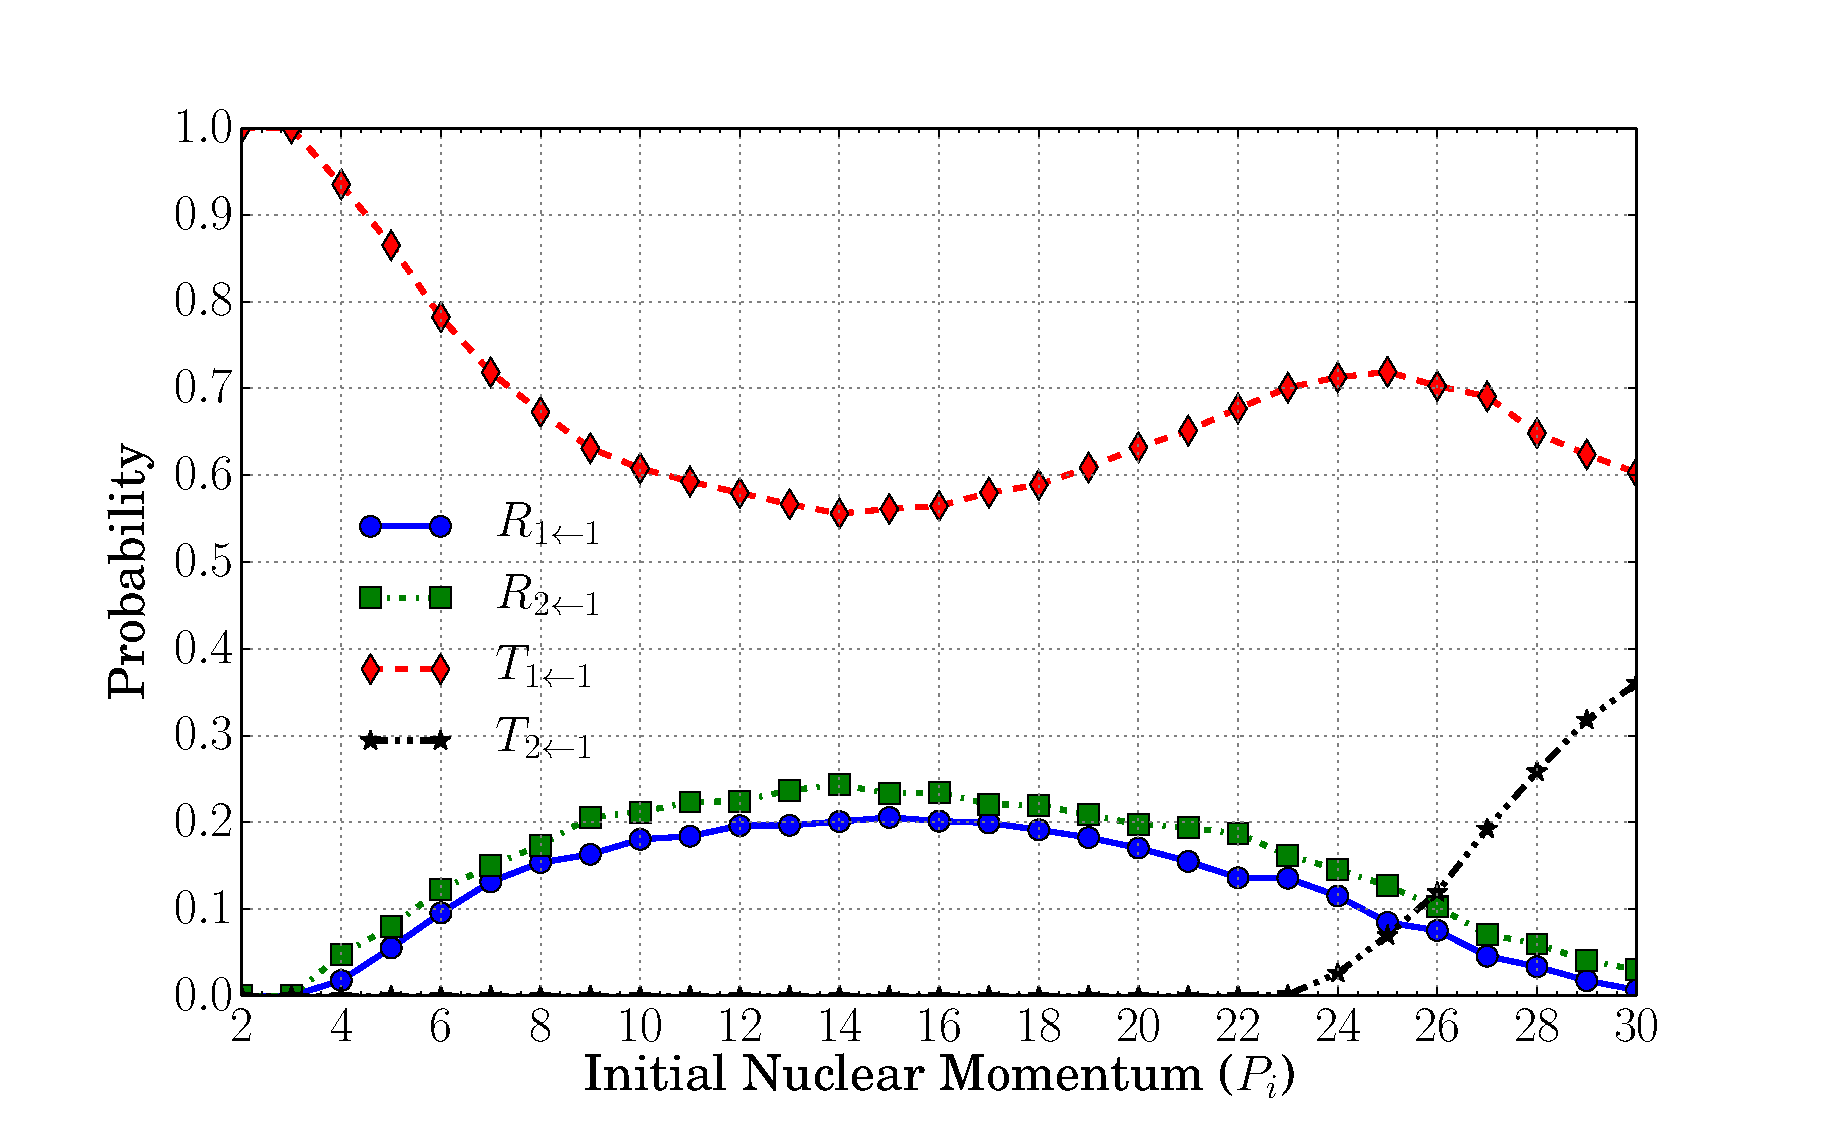
\includegraphics[width=\textwidth]{ec_prob_lh_mean.eps}
\caption[]{Transition probabilities for Reflection ($ R $) and Transmission ($ T $) for $ h = (0.10125 P_{i})^{-1} $, $ 30000 $ MC reps, and initial state $ = 1 $.}
\label{sumf:eci1}
\end{subfigure}
~
\begin{subfigure}[t]{0.5\textwidth}
\centering
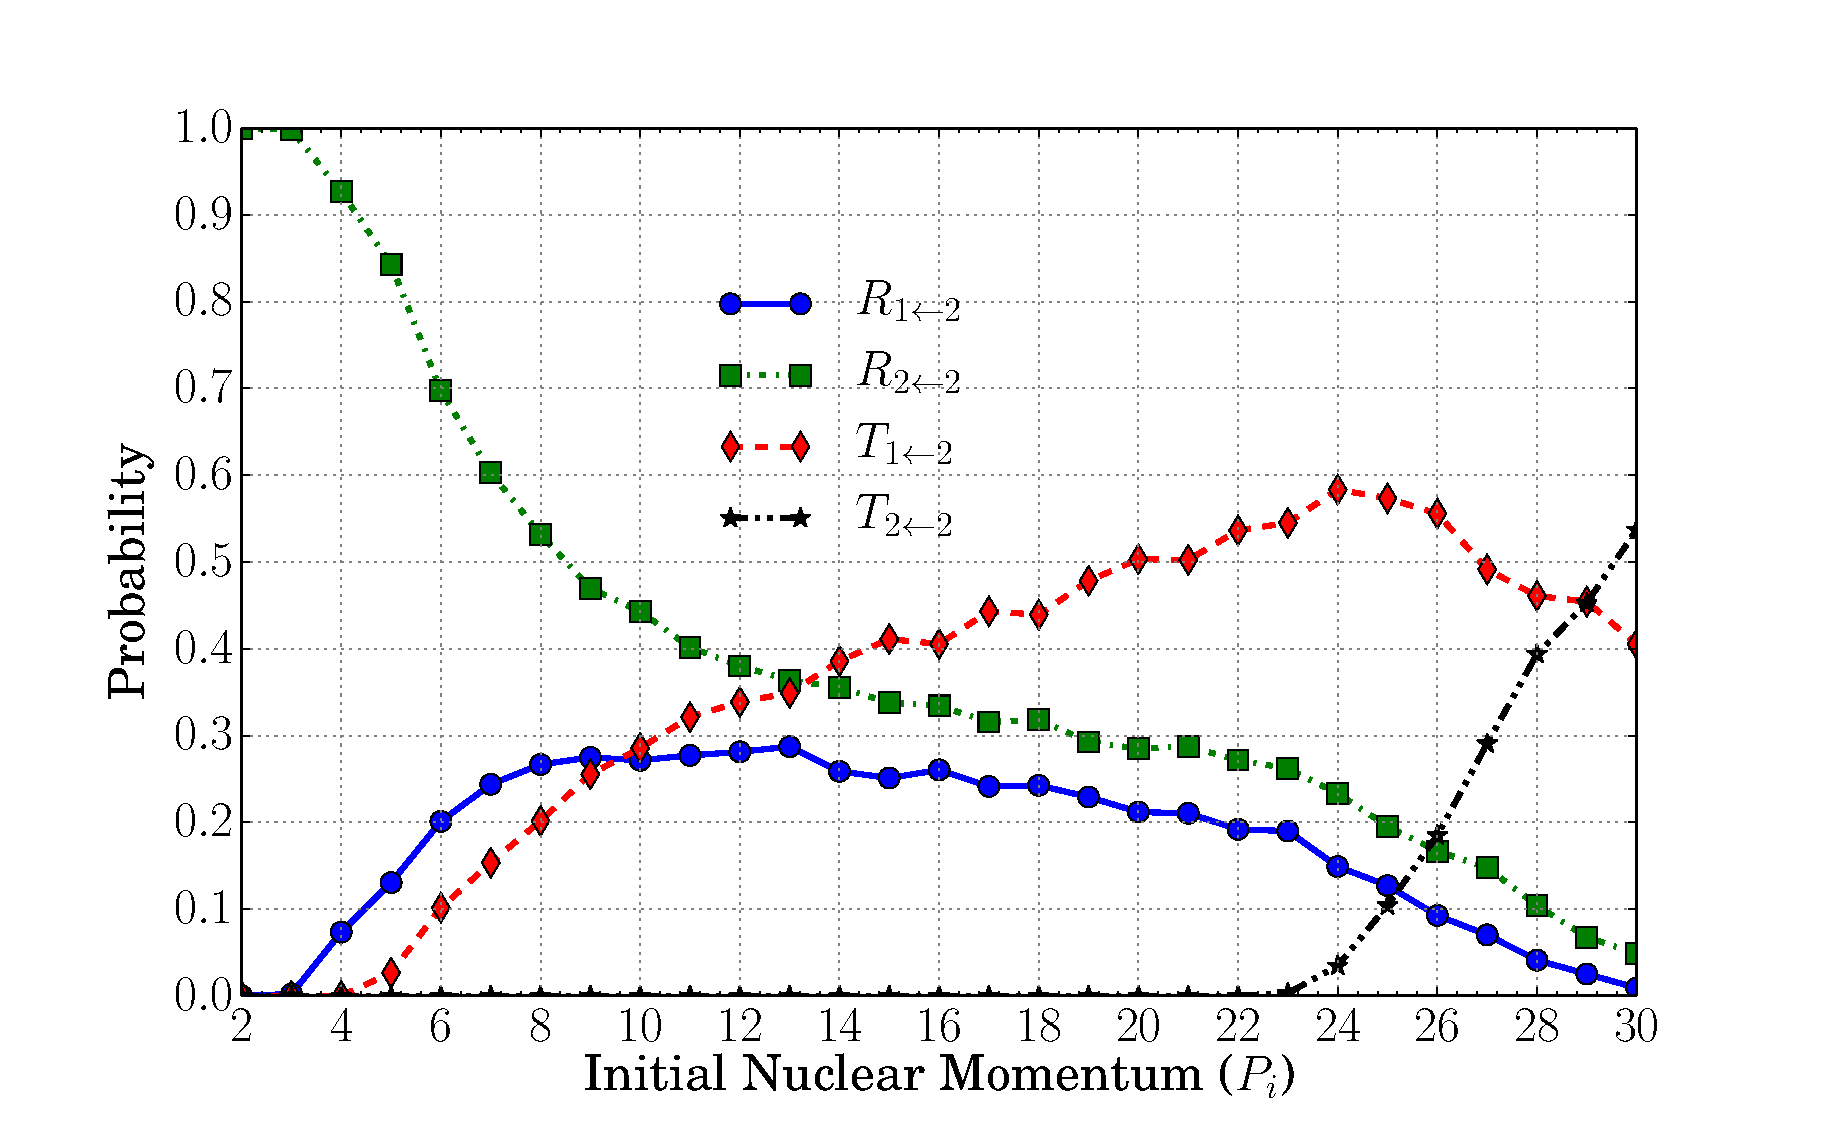
\includegraphics[width=\textwidth]{ec_prob_i2.eps}
\caption[]{Transition probabilities for Reflection ($ R $) and Transmission ($ T $) for $ h = (0.10125 P_{i})^{-1} $ and initial state $ = 2 $.}
\label{sumf:eci2}
\end{subfigure}
\caption[]{Extend coupling transmission probabilities.}\label{sumf:ec}
\end{figure}

Once more, the results for when initial state $ = 1 $ are very similar---but not exactly the same---as those found in \cite{project}. Which can again be attributed to the same factors as before. \Cref{sumf:ec} shows the results for initial states $ = 1, 2 $.

Following previously set precedents, we shall start the analysis with \cref{sumf:eci1} for which initial state $  = 1 $. The behaviour of \too~at low momenta is due to the fact that $ E_{1} $ is highly attractive, so the particle is easily transmitted without strongly interacting with any other PES. However, as the momentum increases the particle starts interacting more strongly with the non-diagonal elements of the hamiltonian matrix, $ H_{12} $, and it becomes more likely to either be reflected by it with or without an electronic transition, giving rise to the bump in probability of \roo~and \rto, and the dip in the probability of \too. It is only at higher nuclear momenta that it is possible for the particle to experience an electronic transition and have enough momentum to work against the repulsive interaction with and $ E_{2} $, leading to a probability increase of \tto.

For the case when the initial state $ = 2 $ (\cref{sumf:eci2}), the system's behaviour changes drastically. At low nuclear momenta, the particle does not have the required energy to be transmitted or undergo an electronic transition, leading to the shape of \rtt. However, as the momentum increases, the particle starts being able to change electronic state and be transmitted, leading to the increase in the probabilities of \rot~and \tot. As the momentum is increased further, the probability of having enough energy to transition into the lower electronic state and be transmitted increases, leading to the drop in \rtt~and \rot, and increase of \tot. As the nuclear momentum increases further, then the particle is travelling fast enough that it can overcome the repulsive effect of $ E_{2} $ and interact relatively little with $ E_{1} $, leading to the increased probability of observing \ttt.
%
\subsection*{Spin-Boson Model for Condensed-Phase Dynamics}
%
\begin{figure}
\begin{subfigure}[t]{0.5\textwidth}
\centering
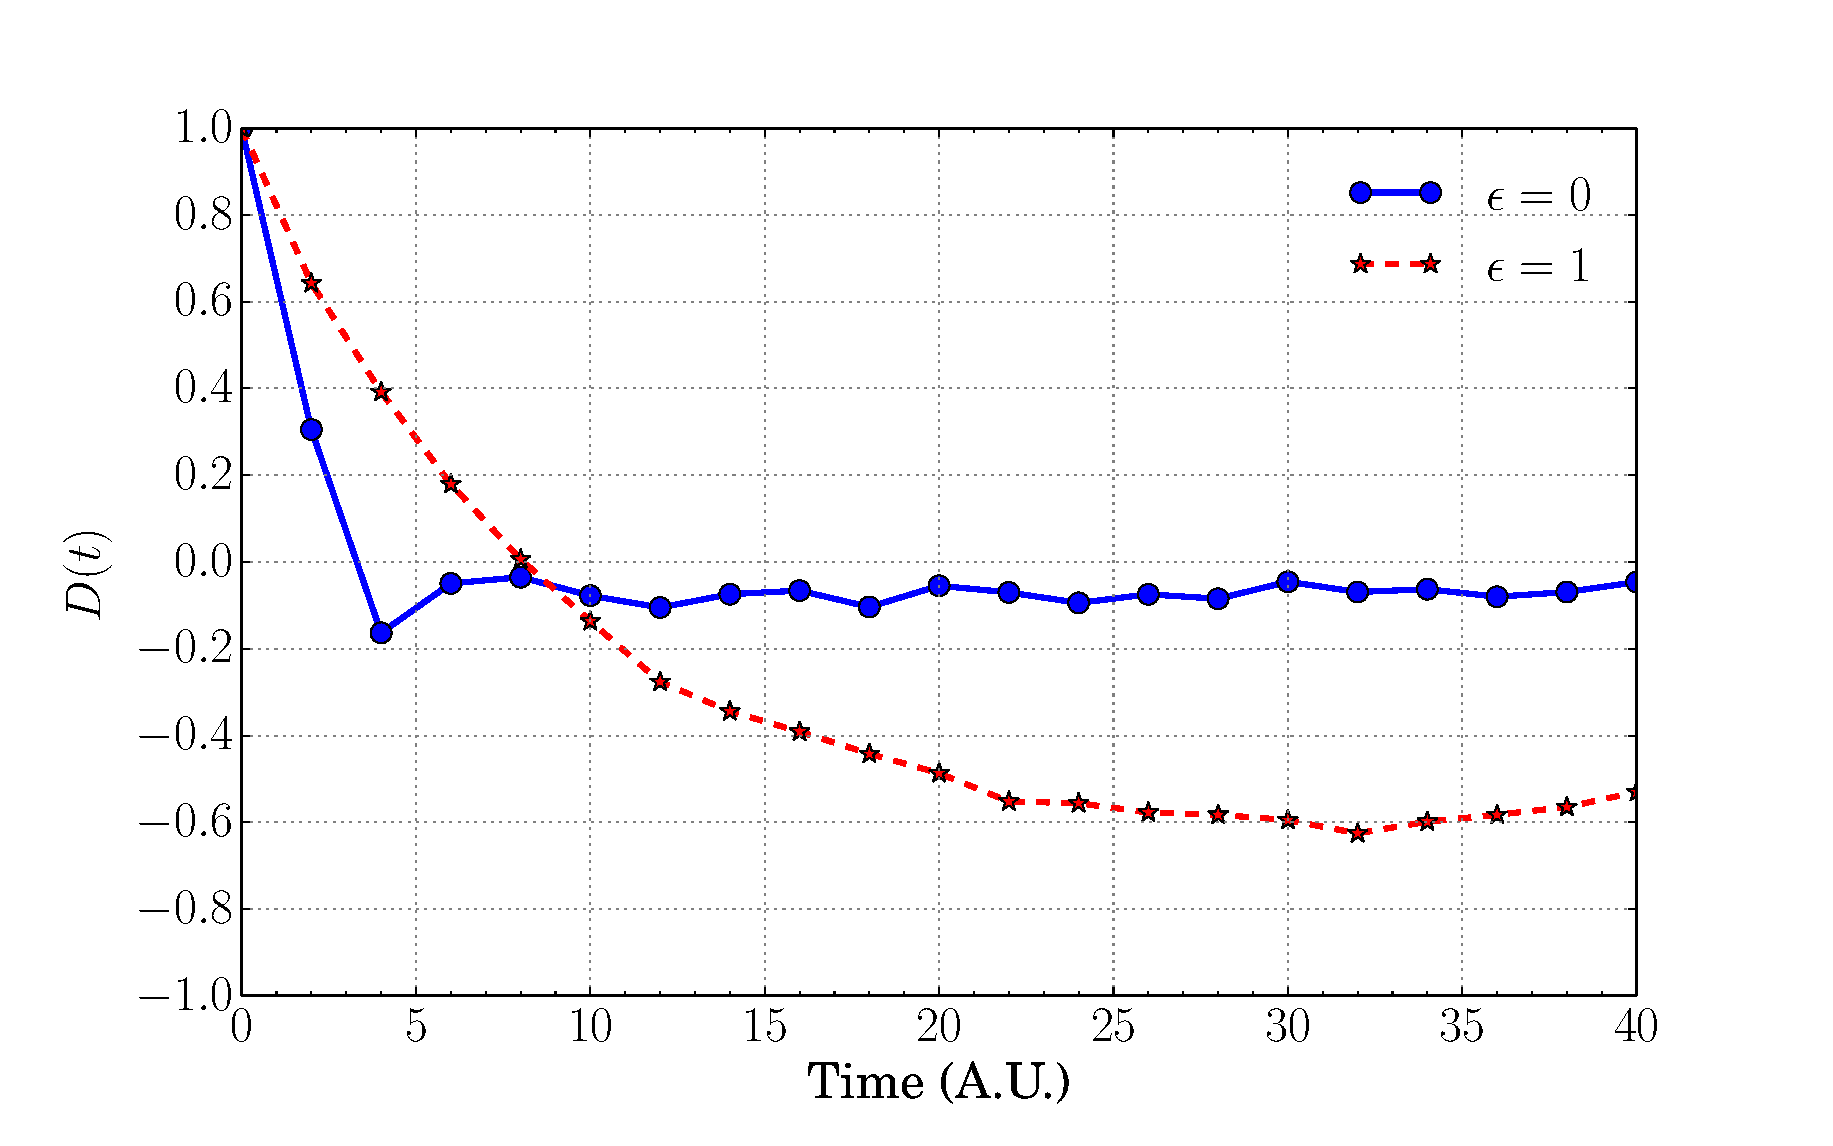
\includegraphics[width=\textwidth]{spin_boson_e11.eps}
\caption[]{Initial state $ = 1$. For both systems $ h = 0.01$.}
\label{sumf:sbe11}
\end{subfigure}
~
\begin{subfigure}[t]{0.5\textwidth}
\centering
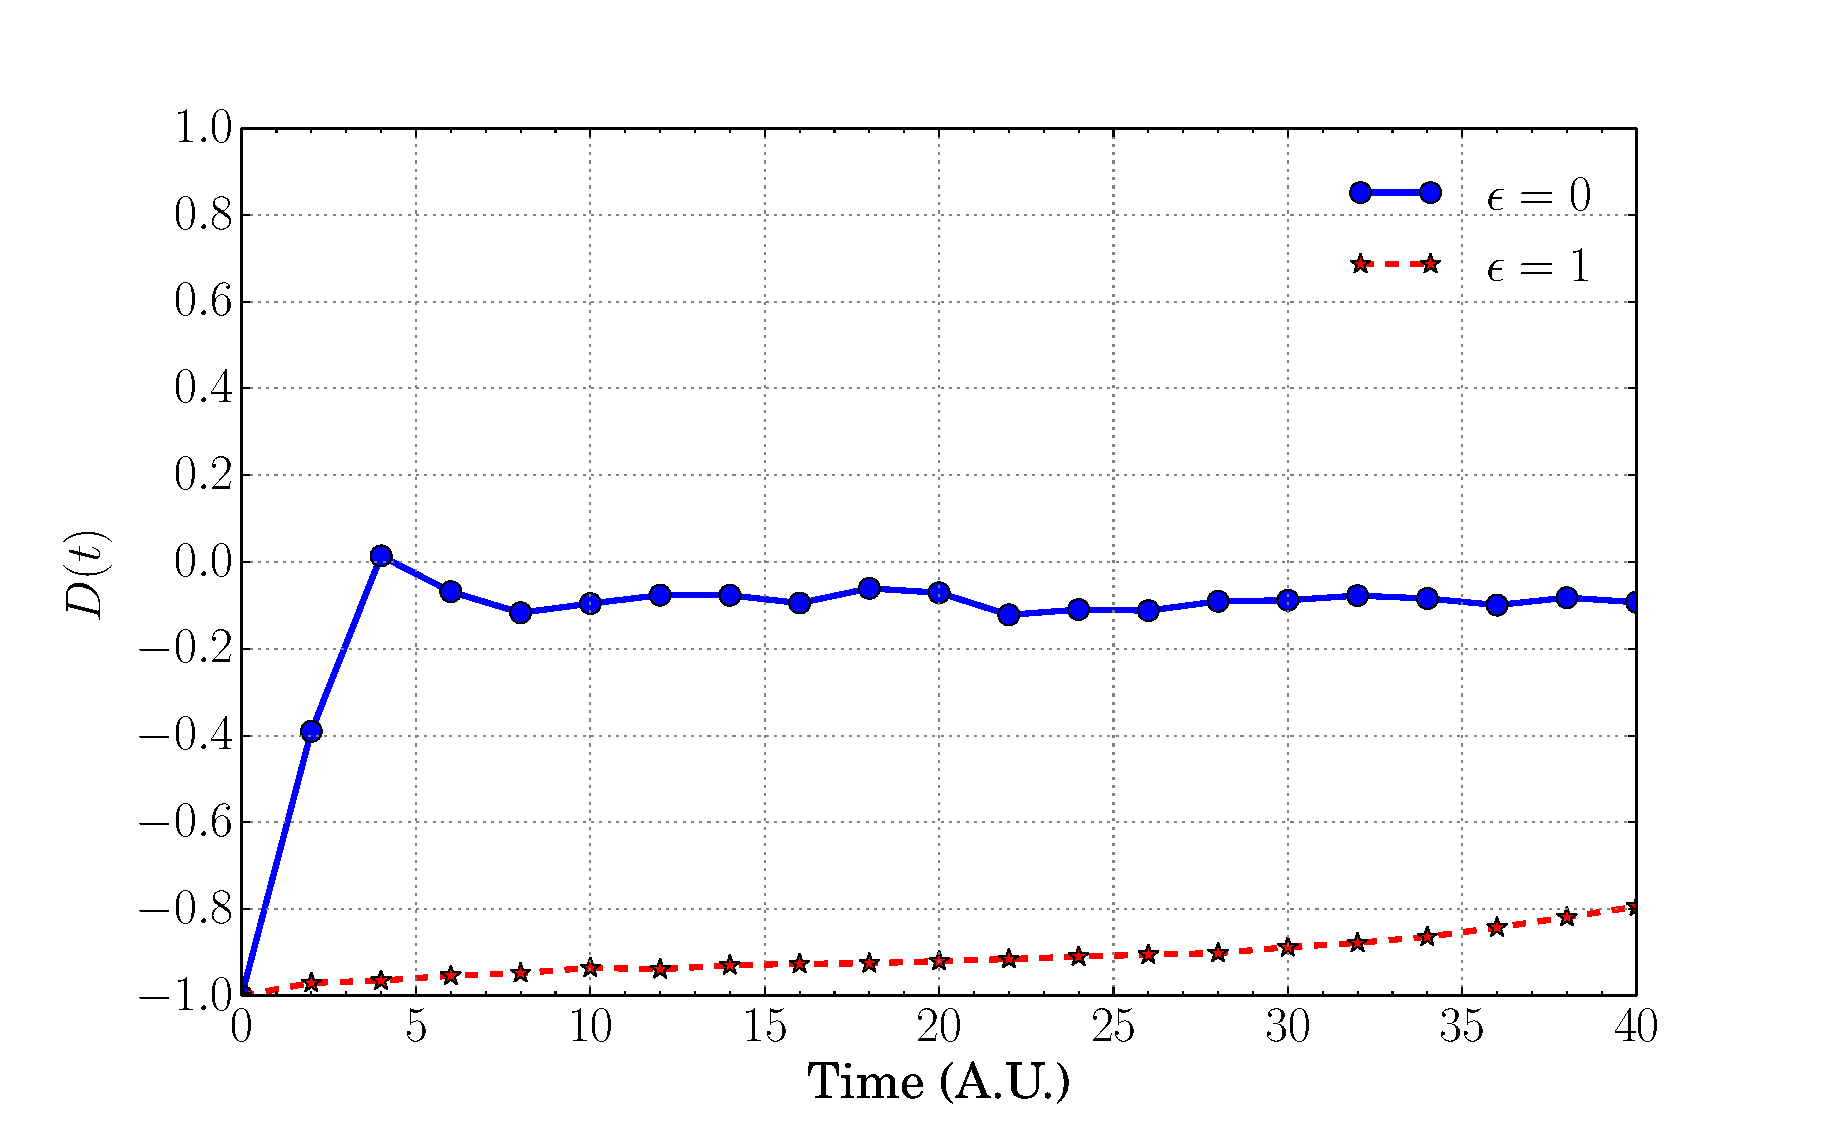
\includegraphics[width=\textwidth]{spin_boson_e12.eps}
\caption[]{Initial state $ = 2 $. For the symmetric problem, $ h = 0.1 $ and MC reps $ = 5000 $. For the asymmetric problem, $ h = 0.01 $ and MC reps $ = 30000 $.}
\label{sumf:sbe12}
\end{subfigure}
\caption[]{Spin-boson calculations for symmetric ($ \epsilon = 0 $) and asymmetric ($ \epsilon = 1 $) systems. $\alpha = 0.09,~\beta = 0.25,~\Delta = (2.5)^{-1}$.}\label{sumf:sb1}
\end{figure}

Some details were left out of \cite{project} in regards to this problem---namely the value of $ \omega_{c} $, and the range and distribution of $ \omega_{k} $---so it was assumed that $ \omega_{c} = 1$ and $ \omega_{k} $ uniformly distributed $\in [0.01\omega_{c},~4\omega_{c}] $ \cite{spin-boson}, and everything else was defined from there; which means there is no standard with which to compare results. \Cref{sumf:sb1,sumf:sb2} show the results of four systems (two symmetric and two asymmetric) characterised by different parameters, for initial electronic states $ = 1, 2 $. The calculations were carried out for 100 nuclei ($ M=100 $).

\Cref{sumf:sb1} shows incoherent (non-oscillatory) relaxation dynamics for all four systems. It is particularly interesting how much the behaviour changes between the symmetric and asymmetric version of each problem. In both cases, the asymmetric system favours the second state. Which means that the second state has a lower energy than the first. This notion is also evidenced by the fact that both symmetric systems stabilise at negative values of $ D(t) $, signifying that the probability of finding the system in state 2 is higher than that of finding it in state 1. This can potentially be observed from \cref{e:sbpes}.

On the other hand, \cref{sumf:sb2} shows both, coherent (oscillatory) and incoherent (non-oscillatory) relaxation dynamics. For both initial states, the symmetric system manifests highly oscillatory behaviours. But the surprising results arise from their asymmetric counterparts. Such results mean that for our chosen parameters, the dynamical system described by the equations of motion has large regions of stability in the electronic phase space. Such phenomena are not unheard of---where the same equations with different parameters yield vastly different results, ranging from nicely behaved to chaotic systems. Suffice to say, this was completely unexpected (and probably highly coincidental).

\begin{figure}
\begin{subfigure}[t]{0.5\textwidth}
\centering
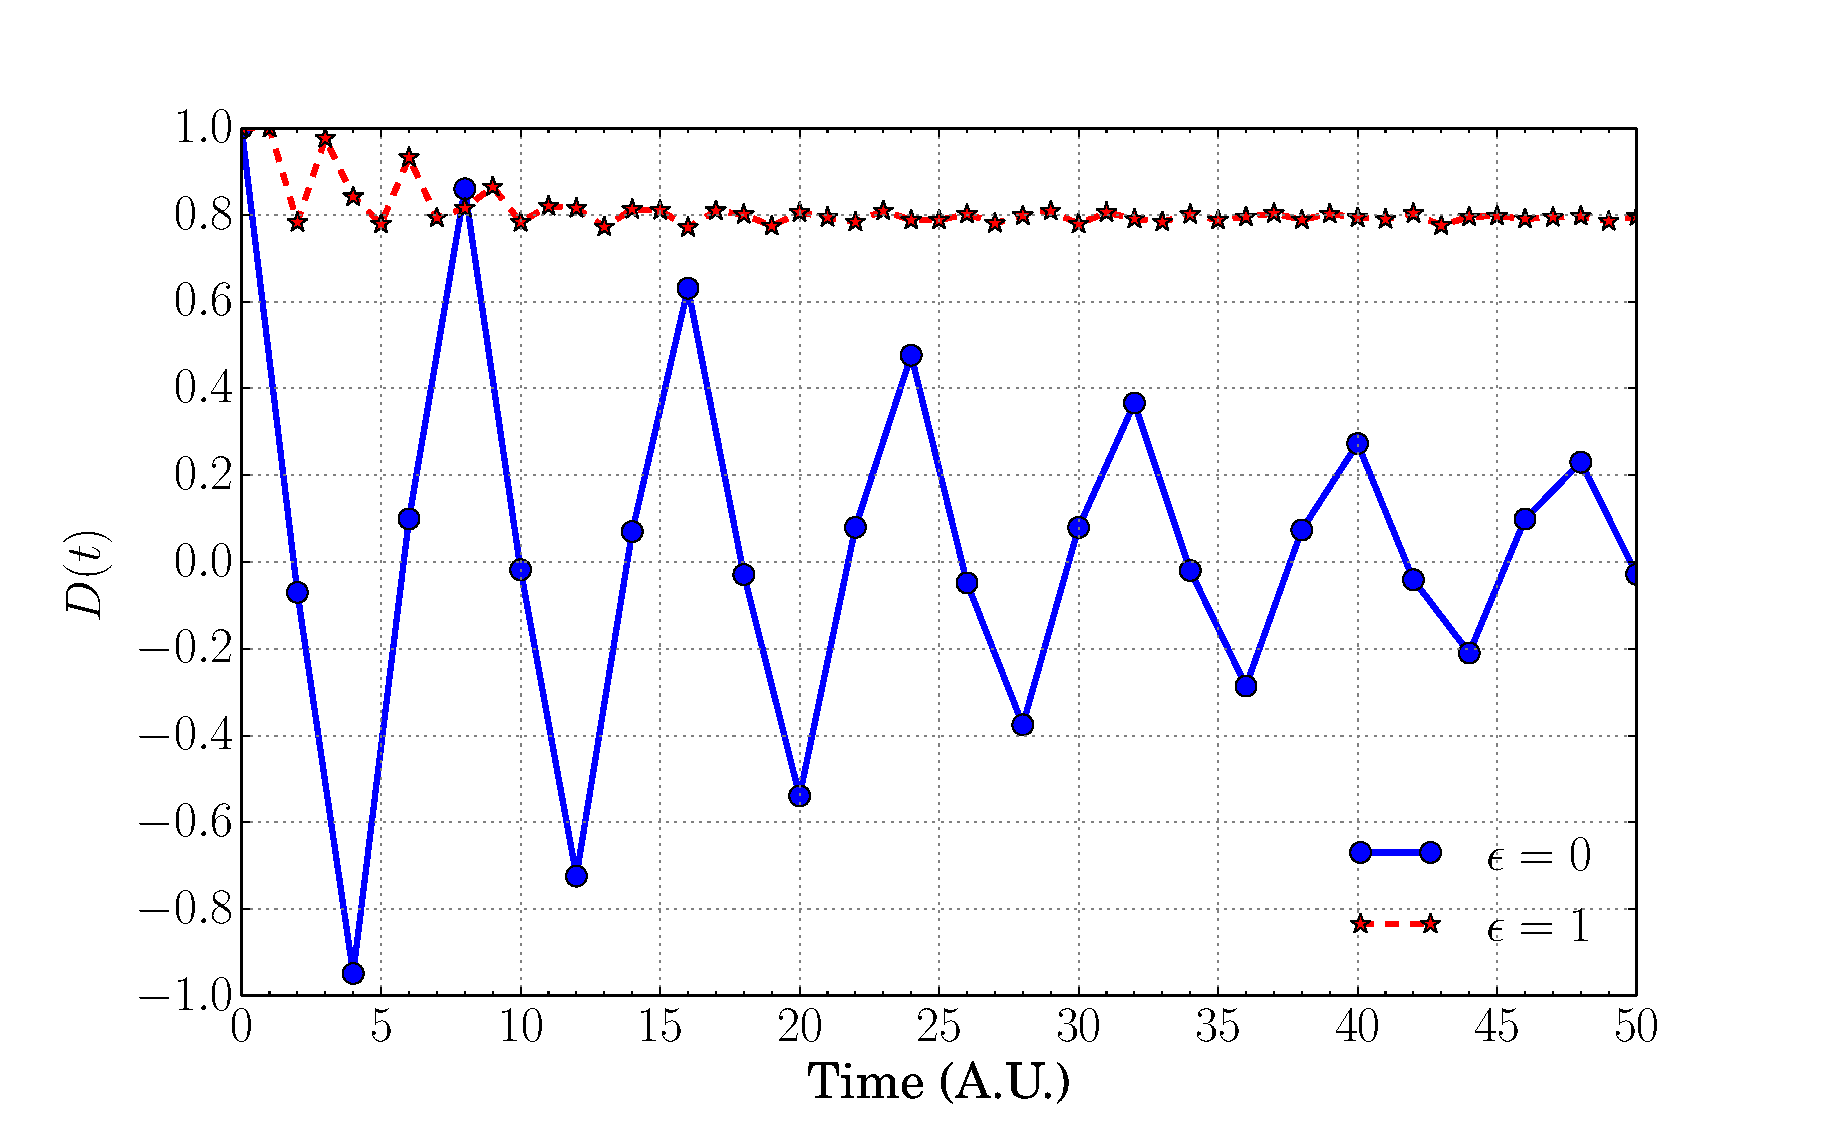
\includegraphics[width=\textwidth]{spin_boson_e21.eps}
\caption[]{Initial state $ =1 $. For the symmetric problem, $ h = 0.1 $ and MC reps $ = 5000 $. For the asymmetric problem, $ h = 0.05 $ and MC reps $ = 30000 $.}
\label{sumf:sbe21}
\end{subfigure}
~
\begin{subfigure}[t]{0.5\textwidth}
\centering
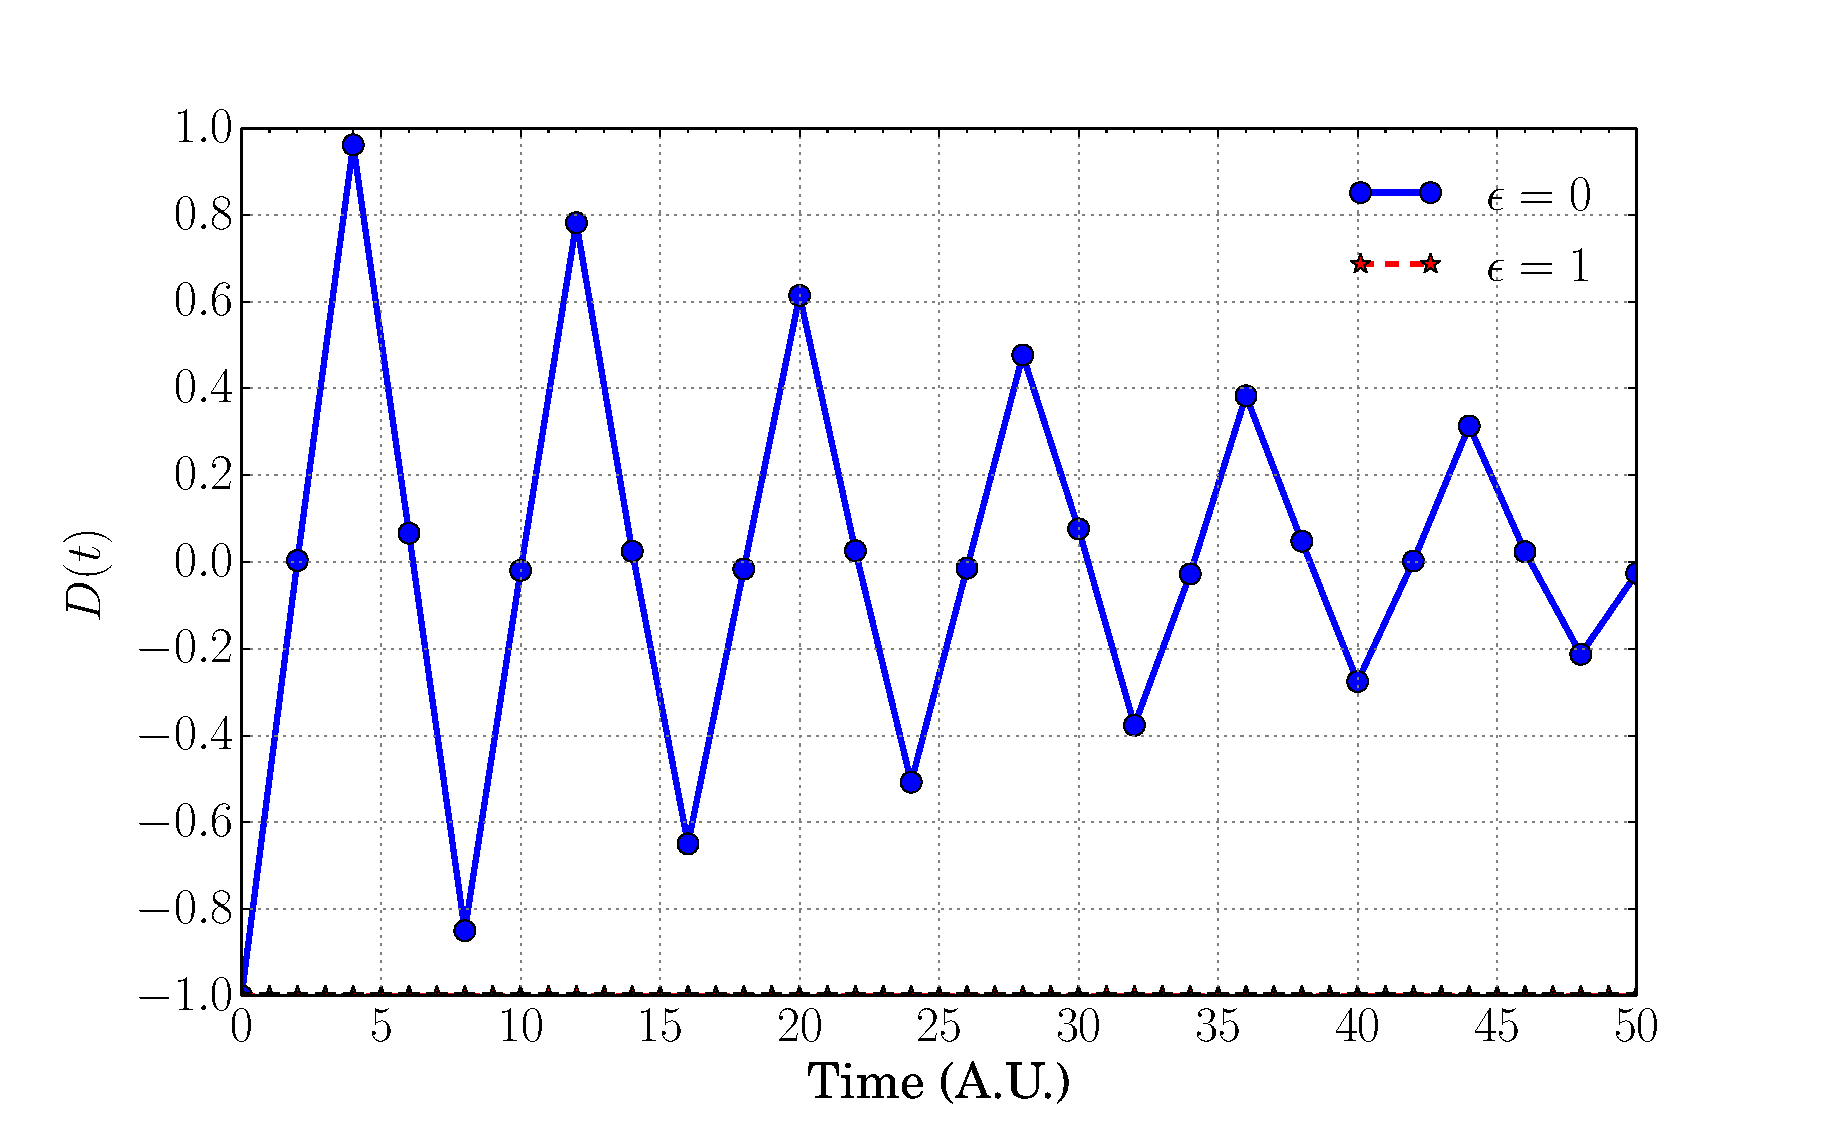
\includegraphics[width=\textwidth]{spin_boson_e22.eps}
\caption[]{Initial state $ = 2 $. For the symmetric problem, $ h = 0.1 $ and MC reps $ = 5000 $. For the asymmetric problem, $ h = 0.05 $ and MC reps $ = 30000 $.}
\label{sumf:sbe22}
\end{subfigure}
\caption[]{Spin-boson calculations for symmetric ($ \epsilon = 0 $) and asymmetric ($ \epsilon = 1 $) systems. $\alpha = 0.1,~\beta = 12.5,~\Delta = (2.5)^{-1}$.}\label{sumf:sb2}
\end{figure}

To conclude with this discussion, it must be said that the disparity in integration step and MC reps is down to each individual system's run time. The aforementioned quantities were adjusted so that no run exceeded 17 hours. There was some overcompensation in a few systems due to the highly variable nature of their run times, which in one instance was observed to exceed $ 250000\% $, though less extreme examples fell in the range of $ 300\%~\text{to}~1000\% $. This phenomenon is attributed to the large number of uniformly and normally distributed random numbers required to set the initial conditions---given that some of them do not allow the selection criteria to be met. The problem was compounded by the random seed allocation at every MC rep, and by the fact that the selection criteria (\cref{e:select}) must be met at every plot point, otherwise the MC rep has to be restarted.
%
\section*{Conclusions}
%
The most recent version of the MM model was successfully implemented in \textsc{fortran 2008}. The code was validated with four simple model systems. New results for all four systems were obtained.
Future work should be carried out to modify the code so it can read input files and be applied to arbitrary systems. The use of an adaptive integration algorithm may also be worth investigating, as it can make calculations faster and more accurate. Lastly, attempts must be made to eliminate the need for analytic PES so the model may be applied to real systems.
%
\setcounter{figure}{0}
\begin{comment}
\clearpage
\newpage
\pagenumbering{arabic}              % Arabic page enumeration.
\setcounter{page}{1}                % Starting page: 1
\thispagestyle{empty}               % Unnumbered first page.
\end{comment}
%----------Acknowledgements---------%
\newpage
\begin{center}
	{\Large\bf{ACKNOWLEDGEMENTS}}
\end{center}
	\vspace{\fill}	
	First, I would like to thank my academic mentors---who I have come to consider my friends. They have been many, their origins and locations span the globe and I cannot name them all, but there are a few who I would like to mention---as their influence on me, I consider the greatest. Starting with Prof. John F. Stanton, who after only two e-mails, told me he would like to be my adviser. If I had been in his position, I would've never risked it on so little information, but I'm glad he did\dots~because it was awesome. My academic adviser, Prof. Marcelo Videa Vargas, for allowing this to happen, and for all the advice and teachings over the years. I'd also like to thank Prof. Anatoly B. Kolomeisky and soon-to-be PhD. Hamid Teimouri for having accepted me as part of the team, as well as for all the help, guidance, advice and philosophical conversation during my 2014 summer internship at the Kolomeisky Group. There's also Prof. Víctor M. Jiménez Pérez, PhD. Concepción ``Conny'' García, PhD. Rodrigo Chan Navarro and Prof. Víctor M. Rosas García, who also welcomed me as part of the team, as well as helped, guided, and advised me during my 2013 summer internship at the Jiménez-Pérez Group. I'd also like to thank Prof. Bernard Micheli Masson, whose classes kept me studying chemistry. Mr. Casserly, whose secondary school chemistry class made me study chemistry, and for helping me develop a critical and objective mind; Mr. Walker, my secondary school ICT teacher, whose words of praise, encouragement and lament over my return to Mexico, I still turn to in times of need and desperation; Mrs. Burrow, Mrs. Milner and Miss Clarke, whose world-views and philosophies I have integrated into my own; and lastly, Mrs. Wade, for all her help when I arrived in a strange, grey land, and upon leaving a grey home.
	
	I also wish to thank \url{www.reddit.com}, \url{www.stackexchange.com} and \url{www.wikipedia.org}, whose communities freely provided me with tools, knowledge and support I could only have otherwise acquired by sinking more money and time into overpriced books, articles and further schooling.
	
	Next in line are my friends---who I have also come to consider my mentors. Namely, I would like to thank \emph{The Spectral League}, \emph{The Disciples}, PhD. Julio L. Palma Anda, and my Senseis Francisco ``Akira'' Espinoza Mancera, Kieth Prole and Sacha Martin-Luther King. The reasons for their appearance here are as varied as they are, but the one thing they all have in common, is that they have bestowed upon me the tools and responsibility to continually improve myself.
	
	And last but certainly not least, my family. And as I have mentioned before, my definition of family is not the traditional definition concerning an arbitrarily defined amount of shared genetic material; but rather that which is given in Disney's \emph{Lilo and Stitch}: ``Ohana means family. Family means nobody gets left behind, or forgotten.'' It is to these people, who have never left my side---or my mind---that I owe the greatest, most heartfelt of thanks. I would name them all, but there is no need, for they instinctively know who they are. I thank you all for making me the person I am\ldots~I hope you've made yourselves proud.
	\vspace{\fill}
%------------Dedication------------%
\newpage
\begin{center}
	{\Large\bf{DEDICATION}}
	
	\vspace{\fill}	
	To my Ohana.
	\vspace{\fill}
\end{center}
%-------------Indexes--------------%
\newpage
\tableofcontents
\newpage
\listoftables
\addcontentsline{toc}{chapter}{Table index \hfill}
\listoffigures
\addcontentsline{toc}{chapter}{Figure index \hfill}
\newpage
\setcounter{page}{1}
%-------------Content--------------%
\pagenumbering{arabic}
%----------Introduction------------%
\chapter{Introduction}\label{c:i}
%
\section{Computational Methods in Chemistry}
%
Computantional chemistry enables the study of chemical systems in ways that traditional techinques cannot \cite{book1}. For example, solvent effects in chemical reactions \cite{ap1} without carrying out the reaction under different solvents and isolating intermediaries. Computational chemistry can also be very valuable for the pharmaceutical industry \cite{pharm7}; particularly the area of cheminformatics, which can greatly speed up the search and sorting of potentially bioactive molecules \cite{pharm2,pharm3}. For example, the discovery DNA gyrase inhibitors with higher affinity than previously known ones \cite{pharm4,pharm5,pharm6}. These techniques are usually extremely fast, for instance, in 2001 a laptop with a 3 GHz processor estimated the ADME \cite{inf} physical properties of 71,500 compounds in 3 minutes using the QikProp package \cite{pharm1}, providing relevant information for further study.

Nowadays, computational chemistry has permeated popular culture in the form of Folding@Home and the Clean Energy Project. Folding@Home currently outputs $48,000$ teraflops of computing power ($ 48,000 \times 10^{12}$ floating point operations per second). F@H focuses on the study of misfolded proteins in Alzheimer's, Huntington's, ALS, Mad Cow, Parkinson's, many cancers, among others \cite{f@h}. On the other hand, the Clean Energy Project focuses on the search and analysis of possible candidates for use in renewable energy projects, and had a cumulative total of 22,564 CPU years up to Jan 17 2014 \cite{cep}.

However, behind the broad range of applications, lie the theory and algorithms which make it all possible. Utilising theoretical techniques and efficient algorithms one can calculate, observe, and explore some of the most fundamental characteristics of chemical systems. Namely: vibrational modes, intermolecular interactions, and electronic structure, all of which can be analysed independently and on different levels of detail \cite{book2}; though sometimes, the problem requires some degree of interdependency.

Computational methods typically fall into four groups \cite{md1,gromacs}:
\begin{inparaenum} [1)\upshape]
	\item \emph{Ab initio} methods start from physical constants and are purely quantum-mechanical, dealing with all the problems N-body interacting systems bring.
	\item Molecular Dynamics (MD) methods apply classical mechanics to chemical systems. They are typically used in the analysis of large-scale systems, where other methods would take too long 	for a small increase in overall accuracy.
	\item Semi-empirical methods use experimental parameters as well as \textit{ab initio} techniques, sacrificing accuracy in the name of speed.
	\item Density Functional Theory (DFT) methods are often mentioned as a subset of \emph{ab initio} methods. DFT methods create a spatially dependent electron density function, reducing the 	problem from N electrons with 3N spacial dimensions to 3 spatial dimensions. Thus greatly reducing computational time. The caveat is that DFT methods are not suitable for strongly correlated 	systems. They can be extended to accomodate time dependency, such methods are called TD-DFT.
\end{inparaenum}

Which method is best suited for one's needs depends on the complexity of the system to be studied, the desired accuracy, and available computational resources \cite{molcas2}. Purely quantum mechanical methods such as \emph{ab initio} and DFT are particularly afflicted by scaling\footnote{\label{fn:1}Scaling is represented by asymptotic notation, $O(f(x))$ \cite{perturbation}, which summarises the computational time dependence as a function of the number of objects to analyse. However, only the function's dominant term is represented \cite{bigo}. For example: $ O(N^{M}) $ means polynomial scaling of order $ M $ \cite{poly_scale}; $O(N!) $ stands for factorial scaling \cite{fact_scale}; $O(C^{N})$ represents exponential scaling \cite{exp_scale}; and $O(M\log(N)) $ logarithmic scaling \cite{log_scale}.} issues \cite{scale}. \Cref{t:scale} shows scaling as a function of the number of atoms and basis set size in the calculation of Coulombic repulsion in two DFT methods \cite{qchem}.

\begin{table}
	\begin{center}
		\caption[Scaling differences in the calculation of Coulombic repulsion in two DFT methods.]{Scaling differences in the calculation$ ^{*} $ of Coulombic repulsion in two DFT methods (times in minutes). The calculations were carried out on alanine oligomers of 5, 10 and 15 amino acids. Scaling as a function of basis set went from $ O(N^{4}) $ to $ O(N^{2}) $ with the new method. Table edited from \cite{qchem}.}\label{t:scale}
	    \begin{tabular}{lcccccc}
    		\hline\\[-4mm]
	    	Basis Set$ ^{\dag} $ & 5(old) & 5(new) & 10(old) & 10(new) & 15(old) & 15(new) \\
		    \hline\\[-4mm]
    		6-31G(df,pd) & 39    & 27    & 145   & 98    & 263   & 169 \\
	    	6-31G+(df,pd) & 109   & 46    & 736   & 160   & 1240  & 362 \\
		    cc-pvdz & 56    & 20    & 177   & 79    & 369   & 143 \\
    		cc-pvtz & 361   & 85    & 1165  & 280   & 2482  & 551 \\
	    	\hline\\[-4mm]
	    \end{tabular}
    \end{center}
    {\footnotesize $ * $ Calculations carried out on a single 2 GHz processor of an Opteron cluster.\\
	$ \dag $ Basis sets in the form of $ X-YZ $G mean that internal orbitals are composed of $ X $ Gaussian primitives (G), while valence orbitals are composed of two functions each; the first is composed of a linear combination of $ Y $ G; the second of a linear combination of $ Z $ G. The + sign indicates the use of diffuse functions, and the parentheses the use of polarisation functions composed of a linear combination of orbital type $ p,~d,~f $ functions as the case may be. Basis sets of the type cc-pv$ n $z where $ n = $ d, t, q$,~ 5,~ 6 \dots $ where (d = double, t = triple, q = quadruple) contain correlation-consistent polarisation functions for valence orbitals; cc-p means `correlation-consistent polarised' and `v' indicates that they only model valence orbitals \cite{book2,basisset1,basisset2}.}
\end{table}

If the algorithms used are perfect, an increase in speed necessarily means a decrease in accuracy---an increase in speed would require the use of mathematical (truncated series, averages, symmetries) and/or physical (locality constraints, potential wells, classical mechanics) shortcuts, as well as the experimental parameters---by simplifying the problem and reducing the total number of operations required \cite{molcas1}. For this reason, the creation of new methods, models and algorithms is of the utmost importance (see \cref{t:scale}). In fact, computational time restrictions are the main reason why semi-empirical and MD methods are widely used in chemical biology and pharmacology \cite{md2,pharm}.

As previously mentioned, molecular dynamics applies classical mechanics to molecular systems. In other words, they apply classical-mechanical principles to systems which require quantum mechanical ones, leading to incomplete and erroneous descriptions \cite{moldyn}. Cases whose scale prohibits a purely quantum treatment, but also require accurate analyses, are analysed with semi-empirical and hybrid models which can extract quantum information (often of semi-quantitative accuracy) from MD simulations. This motivated the creation of the original ``quasiclassical'' model \cite{QC1}, which has traditionally been the easiest way to extract quantum information from MD simulations. It has often (but not always) been of semi-quantitative accuracy, motivating Meyer and Miller to modify and improve it \cite{cmsym}. With said modifications, the Meyer-Miller model (MM), was successfully applied to three non-adiabatic electronic processes originally defined by Tully and a few problems which use the spin-boson model \cite{tully,project}.
%
\section{Meyer-Miller Quasiclassical Trajectory Model with Symmetrical Windowing for Quantum States}\label{s:model}
%
The current iteration of Meyer and Miller's Quasiclassical Nuclear Trajectory Model (MM model) has been tested on four problems: simple avoided crossing, double avoided crossing, extended coupling and the spin-boson model for non-adiabatic dynamics of condensed-phase matter \cite{project}. For the sake of brevity and relevance in \cref{c:i}, it will only be explained in broad terms, a more detailed discussion can be found in \cref{c:mm}.
%
\subsection{Qualitative Description of the Model}\label{sb:qdm}
%
\Cref{c:mm} provides a detailed mathematical description of the model and its modifications, for \cref{c:i} it is enough to describe the general algorithm.
\begin{enumerate}
\item Assign initial positions and states of all atoms involved.
\item Assign initial momentum and action-angle variables of all atoms involved. The initial momentum must be in the direction of the target atom(s).
\item Calculate the initial state window function.
\item Evolve the trajectories with a numerical integration routine. The integration range is defined by the user/problem.
\item Calculate the final state according to the selection criteria.
\item Calculate the final state window function.
\item Save the final state window function for later use in Monte-Carlo averaging.
\item Repeat the process a statistically sensible number of times.
\item Average the initial and final state window functions.
\item Calculate the probability of every event.
\end{enumerate}
%
\section{Proposal}\label{s:p}
%
In order to explore the workings and robustness of the MM model, it will be applied to the analysis of the of four model systems. The model will be implemented in \textsc{fortran 2008} and will eventually be incorporated into the non-commercial computational and quantum chemistry package \textsc{cfour} \cite{cfour}, primarily developed by the Stanton and Gauß research groups. It will be validated by reproducing the results obtained by Meyer and Miller \cite{project}, and used to carry out calculations for different initial states and different conditions for the spin-boson model.

The code will also be generalised as much as possible so it can eventually be added to \textsc{cfour} \cite{cfour}.
%
\subsection{Broad Methodology}
%
The following list of actions is the methodology with which the problem will be tackled.
\begin{enumerate}
\item Obtain equations of motion.
\item Write pseudo-code (list of actions). This is similar to the description given in \cref{sb:qdm} but slightly more detailed.
\item Translate pseudo-code to \textsc{fortran 2008}. This version of \textsc{fortran} was chosen due to its relative ease of use, speed and ample parallelisation potential.
\item Characterise the code.
\item Validate the code by reproducing Cotton and Miller's results \cite{project}.
\item Obtain new results.
\item Generalise the code as much as possible.
\end{enumerate}
%
\section{Conclusions}\label{s:ic}
%
The model has been proven to be of qualitative and quantitative accuracy for the problems defined by Tully \cite{tully,project}, and will be used to generate new results for variations of these systems.

It's worth repeating that the development of different ways of doing things is always worth a fair try. It is why one of the objectives of the present thesis is to sufficiently generalise it so it can eventually be placed at the disposition of the scientific community by including it in \textsc{cfour}.

In all, computational chemistry is a large toolbox with which we can analyse a wide range of phenomena, which would otherwise be inaccessible---or at least---extremely difficult for us to study. And thanks to the wide variety of chemical systems, there is always need to expand it. However, this is \emph{not} the only motivator. The same drivers that haunt and propel all of mankind's endeavours: money, time, ego, efficiency and sheer curiosity; also apply to computational chemistry. For all these reasons, the search for different ways of doing things is of the utmost importance. In a sense, whether these methods work or not, is irrelevant. The fact that they exist and can be used, modified and studied, makes them invaluable for science, as they offer bifurcations in the road to a goal; bifurcations which may lead elsewhere interesting, or---at the very least---provide a different looking-glass through which to see the problem at hand.
\begin{comment}
%
Nature is full of phenomena that according to our intuition and knowledge, should be simple to comprehend, analyse and explain; however closer inspection often reveals the problem to be much more than first impressions let on. Such is the case of the vibronic structure of the \ce{NO3} radical.

The problem has been extensively analised by Stanton, utilising quantum-mechanical methods \cite{no3radical,no3radical1,no3radical2,no3radical3}. Nevertheless, there exists no comprehensive description of it. Which calls for the use of different methodologies in an attempt to do so. Furthermore, the development and/or utilisation of different methods in the analysis of the same problem not only aids in its resolution, but also serves to expand the toolbox known as computational chemistry. The selfsame technique often results in the generalisation, validation, improvement and even development of new methods \cite{tf}.

In order to better illustrate the problem, I ran calculations using \textsc{orca} \cite{orca}, shown later in Chapter \ref{c:i}.

\section{NO$_{3}$}\label{s:no3}

It is generally accepted that \ce{NO3} possesses a planar almost equilateral triangular equilibrium geometry; according to computational and experimental evidence, it presents a slight $ \mathbf{D_{3h}} \rightarrow \mathbf{C_{2v}} $ deformation \cite{no3radical1}.

\subsection{Role of NO$_{3}$ in Atmospheric Chemistry}\label{sb:atm}

\begin{figure}[t]
	\centering
	\includegraphics[width=\textwidth]{atm.eps}
	\caption[Role of \ce{NO3} in the Atmosphere.]{Role of \ce{NO3} in the Atmosphere. Diagram obtained from \cite{no3origin}.}\label{no3atm}
\end{figure}
\ce{NO3} plays an important part in atmospheric chemistry as shown in \ref{no3atm}. It is an integral part of the nitrogen, carbon and ozone cycles. Such a wide influence makes it of particular importance to life on earth---which would simply be impossible to maintain in its current form if any cycle were to be severely disturbed.

\ce{NO3} is generated from ozonolisis of nitric oxides. The reaction predominantly occurs at night because UV light catalyses the inverse reactions. It plays an important role in vegetated areas---where it oxidises and nitrates terpenes, isoprenes and alquenes emitted by vegetation; oceanic regions---where it reacts with dimethyl sulphoxide released by phitoplankton; and urban environments---where it reacts with nitrogen oxides emitted by human activity \cite{no3origin}.

\section{Vibrational Modes}\label{s:vm}

In order to properly define vibronic structure we must first understand vibrational modes. These are the relative movements of one or more atoms with respect with the rest. They are a direct consequence of the Heisenberg uncertainty principle, which states that the more one knows of a particle's momentum, the less one knows of its position $ \sigma_x \sigma_p \leq \frac{\hbar}{2}$, where $ \sigma = \text{standard deviation} $, $ x = \text{position} $, $ p = \text{momentum} $ and $ \hbar = \frac{h}{2 \pi} $ known as the reduced planck constant. The uncertainty principle is a direct consequence of the wave-like nature of quantum particles. In simpler terms, in order to know the precise momentum of a wave, one has to look at a large space; in doing so, one looses information on the particle's precise position. Likewise, if we only look at a small space we can acquire precise information of the particle's position, but not its momentum. The mathematical reason for this is that a wave's momentum ($ p $) is related to its frequency (it is the Fourier transform from the position domain into the frequency domain) and for wave-like particles, this frequency ($ \nu $) is related to the de Broglie wavelength ($ \lambda $) by $ p = \frac{h}{\lambda} = \frac{E}{c} = \frac{h \nu}{c}$ where $ E = \text{energy} $ and $ c = \text{speed of light} $.

The number of vibrational modes in a non-linear molecule is $ 3N-6 $, where $ N $ is the number of atoms. The formula is derived from observing that each atom has 3 degrees of liberty $ (x,y,z) $, from where $ 3N $ comes from. But there exist a number of linear combinations of movements which keep the molecular geometry unchanged (the relative position of all atoms remains unchanged), but change their absolute position. These include: movements along three axes, and rotations about them---giving a total of 6 degrees of movement which preserve molecular geometry. For linear molecules the number of modes is $ 3N-5 $ because rotations about the main axis do not change a molecule's geometry. The specific shape of each movement depends on the molecule's symmetry group.

Vibrational modes can be experimentally observed through the use of Raman and Infrared (IR) spectroscopy. Raman-active modes are those which modify the molecule's polarisability , while infrared active modes are those which modify its dipole moment\footnote[2]{S. Thomas, ``Infrared and Raman Spectroscopy''. \url{http://serc.carleton.edu/NAGTWorkshops/mineralogy/mineral\_physics/raman\_ir.html}}. The frequency (IR) or shift (Raman) at which modes are observed, depend on the atoms and bond types involved. For our present purposes, we are only interested in IR-active modes.

\subsection{Infrared Spectroscopy}\label{sb:ir}

The main problem presented by \ce{NO3} is that its vibrational modes do not correspond to the experimental evidence. Its IR spectrum is much more complex than it should (see Table \ref{t:spec1}). However, before going into further detail, it would be useful to understand an simple example. Figure \ref{f:form} showcases two spectra of formaldehyde, one simulated and another experimental.

\begin{figure}[t]
	\centering
	%\resizebox{1.0\textwidth}{!}{\input{irform}}
	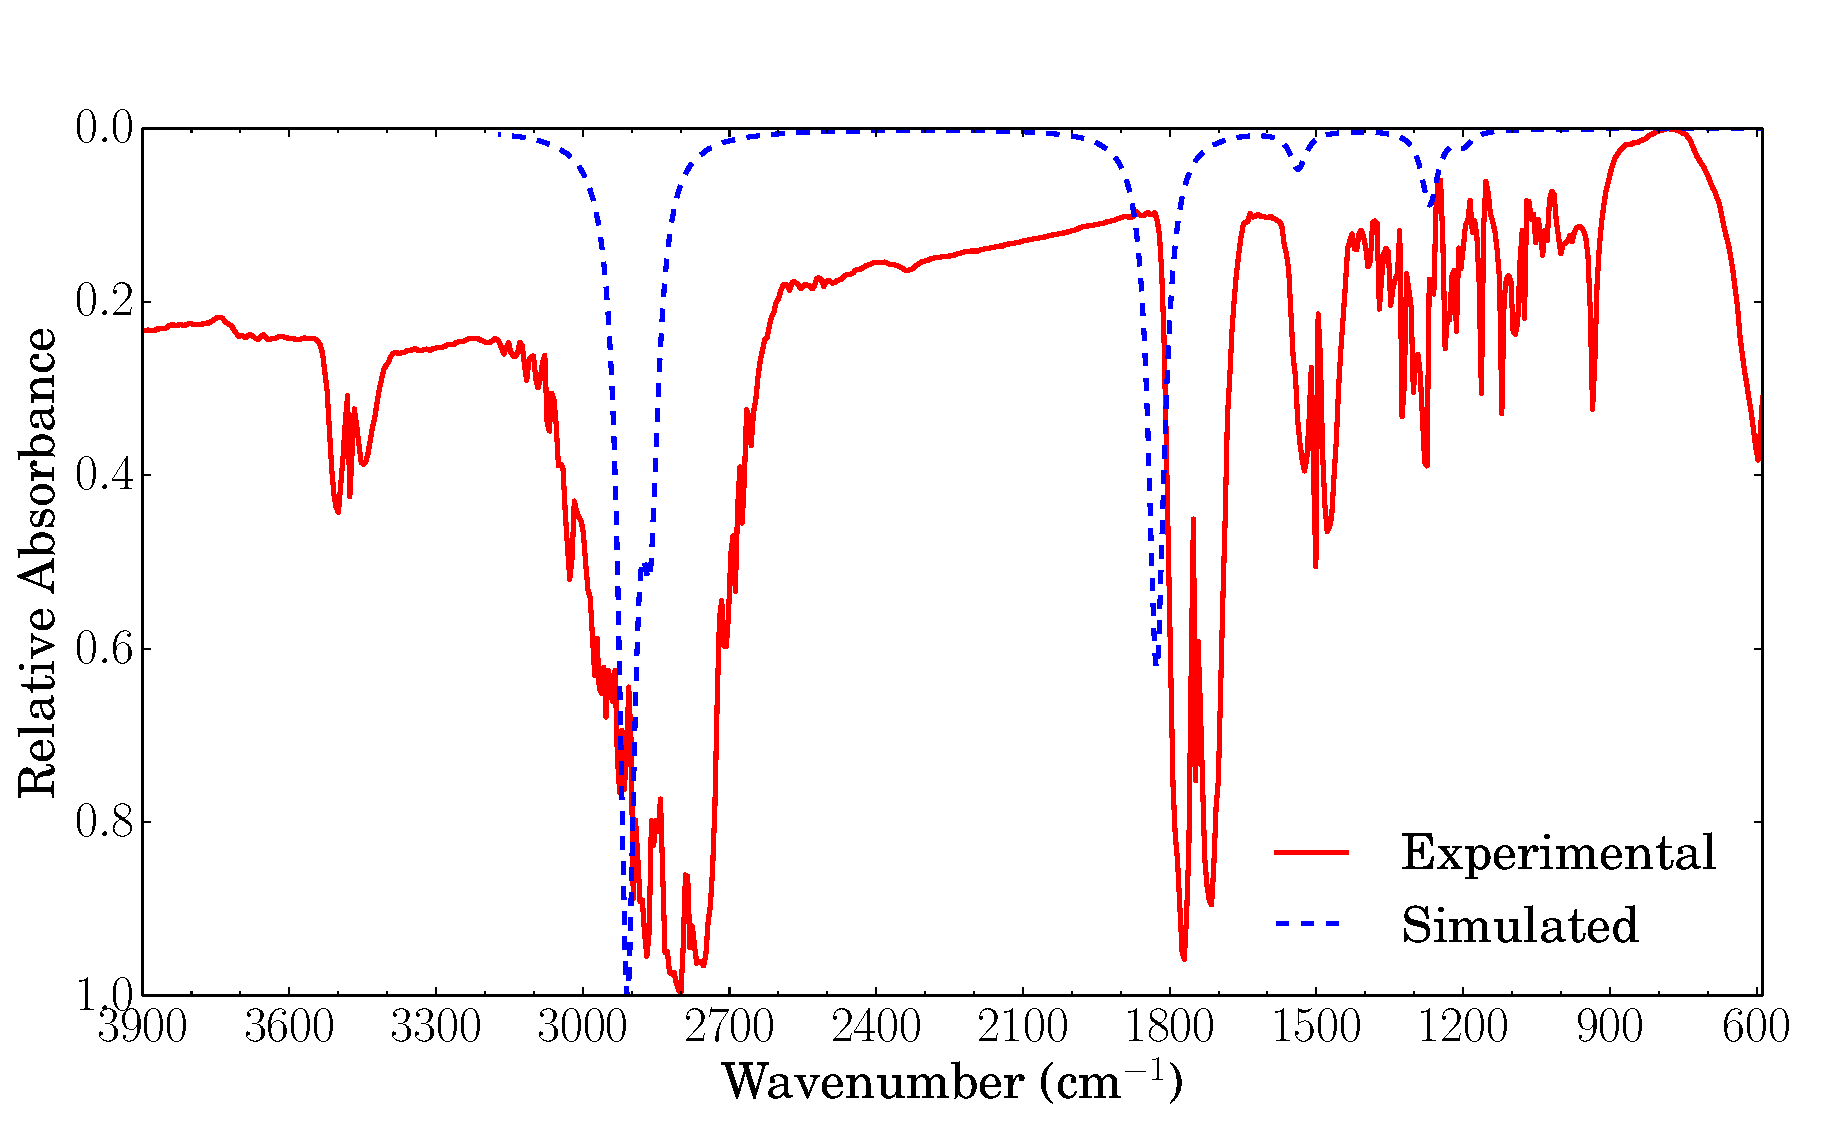
\includegraphics[scale = 0.5]{irform.eps}
	\caption[Simulated and experimental IR spectra of formaldehyde.]{Simulated (solid red line) and gas-phase experimental (dotted blue line) IR spectra of formaldehyde. Simulated spectrum calculated with \textsc{orca} using \textsc{sto-6311g** dft/b3lyp} \cite{orca}. Data for the experimental spectrum obtained from \cite{formgasir}.}
	\label{f:form}
\end{figure}
In this kind of spectroscopy, organic molecules' bonds' vibrational energy and the incident photon's energy are approximately 1 order of magnitud from one another. Furthermore, it requires the presence of a permanent or induced dipole moment (dipole moment different to zero\footnote[3]{$ \mathbf{p(r)} = \sum\limits_{i=1}^{N} q_{i} (\mathbf{r}_{i} - \mathbf{r}) \neq 0$, where $ q_{i} $ is the charge $ i $ and $ \mathbf{r}_{i} $ its position with respect to the observation point $ \mathbf{r} $ (commonly the centre of mass).}) which changes during the vibration. This type of spectroscopy is classified as absorptive, given that the photon's energy is absorbed by the by the bond, and its energy transferred into the vibrational process.

The discrepancies seen in Figure \ref{f:form} are due to various reasons. Two of which can be traced to the number of molecules involved in either case. In simulation, one analyses an isolated molecule, which is why all peaks are clearly defined. Experimentally, that is impossible, so there are bound to be interactions between the involved molecules. Aggravatingly (in this case), if there is trace water--very likely considering it's formaldehyde--condensation reactions can occur, leading to the formation of a variety of oligomers. These interactions and reactions complicate the spectrum, broadening, intensifying, dampening and even creating new peaks. The third reason as to why experimental and simulated spectra differ is vibronic structure, which will be simply explained in \ref{sb:vib}.

\subsection{IR Spectrum of NO$ _{3} $}\label{sb:irno3}

Table \ref{t:spec1} shows the experimental and simulated IR spectra of \ce{NO3}, as well as their band assignations and vibrational classification. Figure \ref{f:irteono3} shows a simulated \ce{NO3} IR spectrum.s:ic
\begin{table}
	\centering
	\caption[Experimental and simulated IR spectrum and frequency assignation of \ce{NO3}.]{Experimental and simulated IR spectrum and frequency assignation of \ce{NO3}. Where $ \nu_{1} $ is a totally symmetric N--O stretching; $ \nu_{2} $ an out-of-plane bending; $ \nu_{3} $ a degenerate N--O stretching; and $ \nu_{4} $ a degenerate in-plane bending. $ \updownarrow $ denotes parallel bands and $ \leftrightarrow $ perpendicular ones \setcounter{footnote}{3}\protect\footnotemark. Table edited from \cite{no3radspec}.}
	\label{t:spec1}
	\begin{subtable}{\textwidth}
		\centering
		\caption{Experimental vibrational modes of \ce{NO3}.}\label{t:exp}
    	\begin{tabular}{rccl}
        	\hline\\[-4mm]
	    	Band & $I$ & \multirow{2}[2]{*}{Type} & Vibrational \\
    		(cm\textsuperscript{-1}) & (Relative) &       & Assignment \\
        	\hline\\[-4mm]
	    	759   & 0.3   & $\updownarrow$ & $\nu_{2}+\nu_{4}-\nu_{4}$ \\
    	    762   & 0.8   & $\updownarrow$ & $\nu_{2}$  \\
    		1492  & 4.7   & $\leftrightarrow$ & $\nu_{3}$ \\
	    	1927  & 3.0   & $\leftrightarrow$ & ?      \\
    		2024  & 1.5   & $\leftrightarrow$ & $5\nu_{4}$  \\
    		2155  & 2.0   & $\leftrightarrow$ & $\nu_{1}+3\nu_{4}$  \\
	    	2200  & 0.7   & $\leftrightarrow$ & ?    \\
    	    2240  & 0.4   & $\leftrightarrow$ & ?      \\
    		2380  & 0.4   & $\leftrightarrow$ & ?     \\
	        2518  & 2.1   & $\leftrightarrow$ & $\nu_{1}+\nu_{3}$ \\s:ic
    		2585  & 1.7   & $\leftrightarrow$ & $2\nu_{1}+3\nu_{4}$ \\
    		7602  & 0.14  & $\updownarrow$ & $\nu_{4}$ \\
	        7744  & 0.4   & $\leftrightarrow$ & $\nu_{2}$   \\
    	    \hline\\[-4mm]
        \end{tabular}
	\end{subtable}
	\\[0.5cm]
	\begin{subtable}{\textwidth}
		\centering
		\caption{Vibrational modes calculated using \textsc{orca} with \textsc{sto-6311g** dft/b3lyp} \cite{orca}.}
    	\begin{tabular}{cccc}
		    \hline\\[-4mm]
			Band & $I$ & \multirow{2}[2]{*}{Type} & Vibrational \\
			(cm\textsuperscript{-1}) & (Relative) &       & Assignment \\
			\hline\\[-4mm]
			$ 259 $   & $ 0.898 $ & $ \leftrightarrow $ & $ \nu_{4} $\\
			$ 293 $   & $ 1 $ & $ \leftrightarrow $ & $ \nu_{4'} $\\
			$ 801 $   & $ 0.898 $ & $ \updownarrow $ & $ \nu_{2} $\\s:ic
			$ 1118 $ & $ 0.005 $ & $ \leftrightarrow $ & $ \nu_{3} $\\
			$ 1133 $  & $4 \times 10^{-4}$ & $ \leftrightarrow $ & $ \nu_{1} $\\
		\hline\\[-4mm]
		\end{tabular}\\
	\end{subtable}
\end{table}

\begin{figure}[t]
	\centering
	%\resizebox{1.0\textwidth}{!}{\input{irtno3}}
	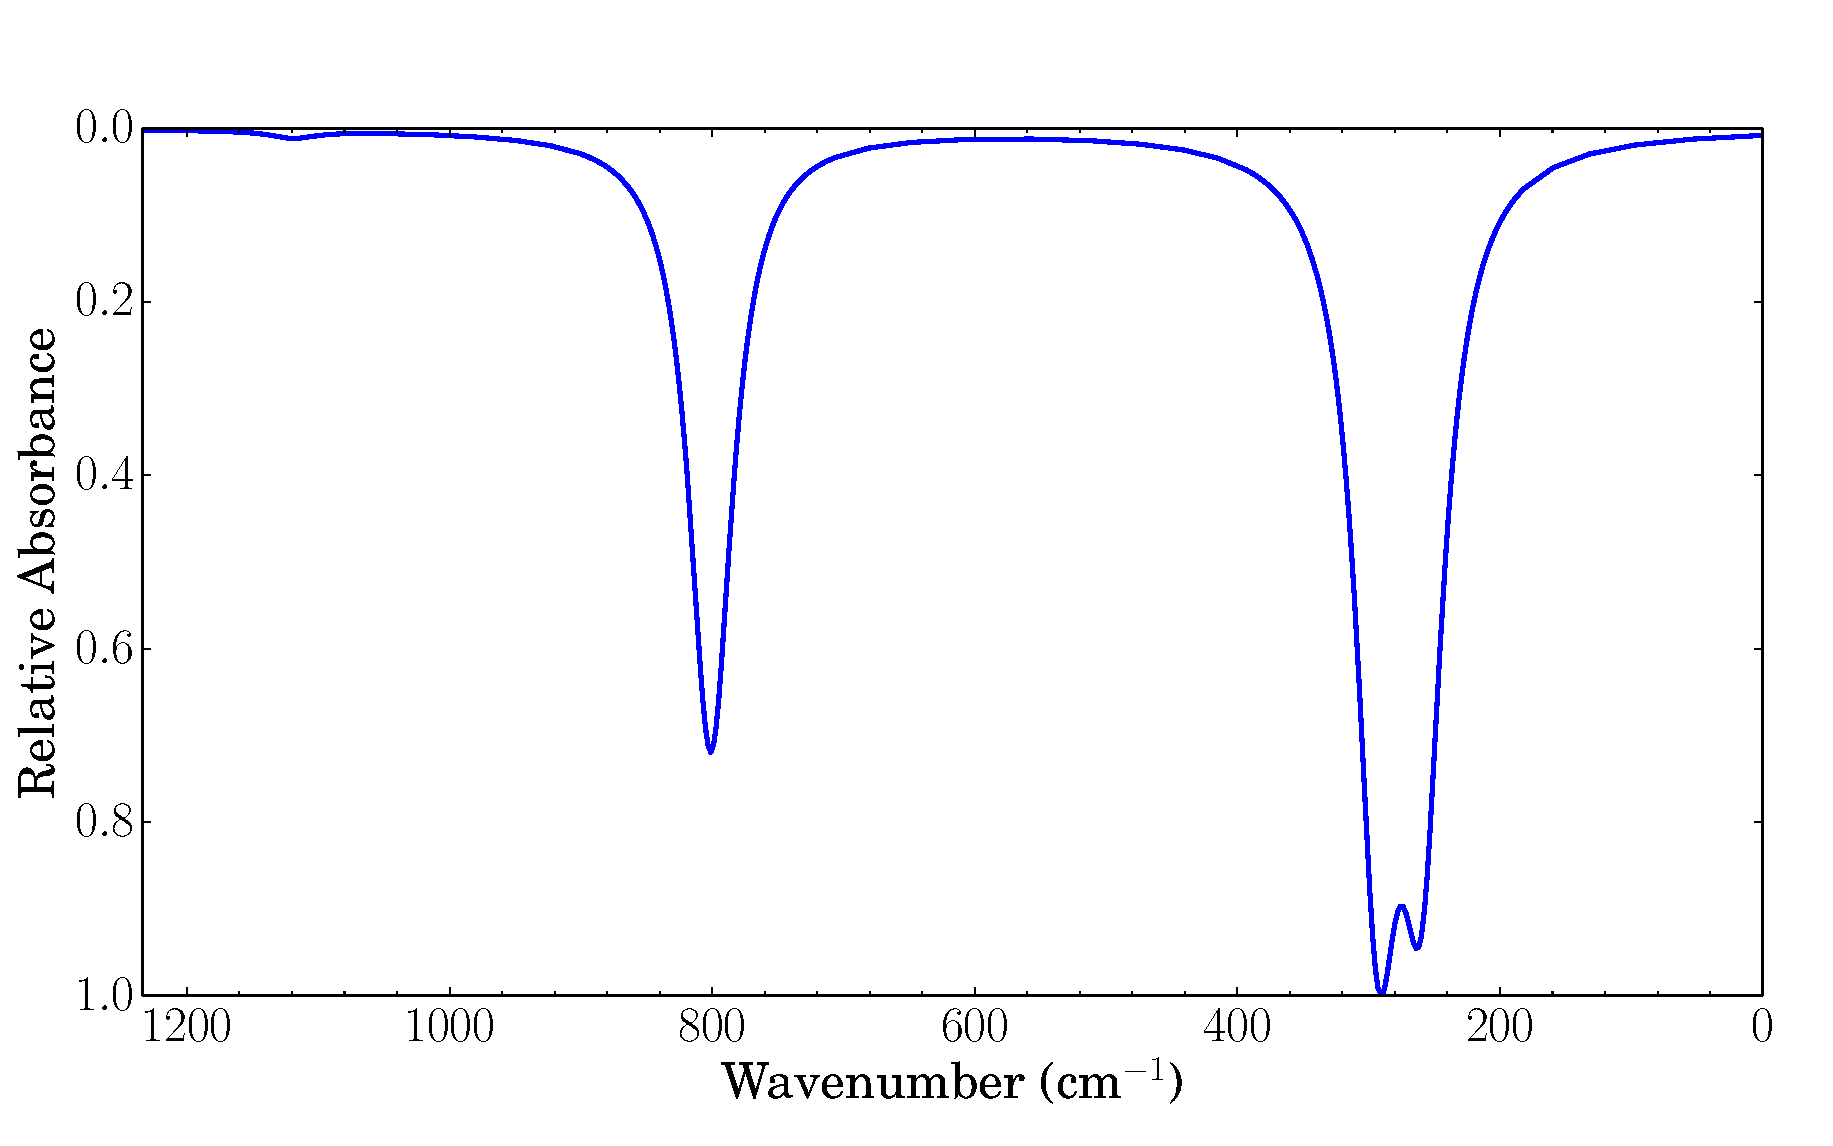
\includegraphics[scale=0.5]{irtno3.eps}
	\caption[Simulated IR spectrum of \ce{NO3}.]{Simulated IR spectrum of \ce{NO3}. Calculated using \textsc{orca} with \textsc{sto-6311g** dft/b3lyp} \cite{orca}.}
	\label{f:irteono3}
\end{figure}

It is evident from Table \ref{t:spec1} that there exists no significant correlation between simulation and experiment. The only band which is relatively in close in all categories is an out-of plane bending parallel band that appears at 801 and 762 cm\textsuperscript{-1} in the simulated and experimental spectra respectively. Additionally, the simulations erroneously indicate the existence of a single degenerate mode, $ \nu_{3} $, when in reality there are two, $ \nu_{3} $ and $ \nu_{4} $ \cite{no3radspec}. These discrepancies are too large to be solely attributed to intermolecular interactions, which broaden and displace peaks, but preserve the general spectral structure, just as in Figure \ref{f:form}. In this case, however, both spectra are completely different.

\footnotetext{\label{fn:3}A band is classified as perpendicular if the change in the dipole moment is perpendicular to its major rotational axis. Likewise, it is classified as parallel when the change is perpendicular to the major rotational axis.}
\subsection{Vibronic $ \equiv $ Vibrational $ \oplus $ Electronic}\label{sb:vib}

The concept of vibronic structure deals with the relationship between vibrational and electronic states. Figure \ref{f:vibronic} is a simple, fictitious diagram that illustrates the concept.
\begin{figure}[t]
	\centering
	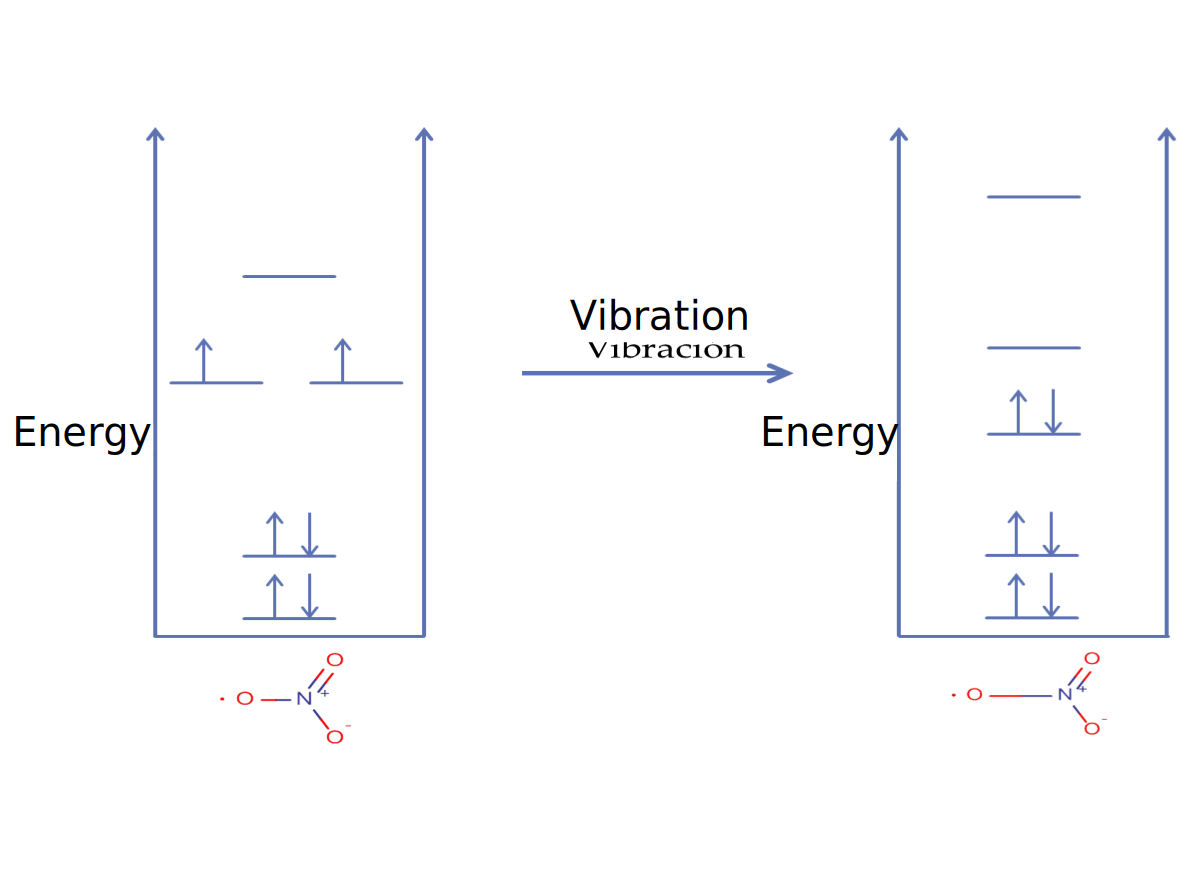
\includegraphics[width=\textwidth]{vibronic.eps}
	\caption[Diagram of a fictitious vibronic structure.]{Diagram of a fictitious vibronic structure. Horizontal bars indicate electronic states, arrows indicate electrons and their spin.}
	\label{f:vibronic}
\end{figure}
Initially, a molecule finds itself in its equilibrium geometry. Suddenly, one of the bonds absorbs a photon, whose energy is transferred into the bond as a vibration which changes the molecule's geometry (and possibly symmetry), consequently so do the shapes and energies of its molecular orbitals (MOs). In the diagram, both degenerate orbitals (orbitals with the same energy) change their energies, and so does the molecule's multiplicity. These relatively drastic changes of energy, multiplicity and symmetry open the floodgates to a myriad of previously inaccessible vibrational modes. To compound the issue, the process can repeat itself indefinitely, giving rise to the final jumble of vibrational modes observed experimentally in Table \ref{t:spec1}.

This problem has been extensively researched from a purely quantum-mechanical perspective by Stanton \cite{no3radical,no3radical1,no3radical2,no3radical3}. However, this type of analysis is extremely complicated and laborious, as it entails carrying out time-dependent calculations of simultaneous, interacting processes. For this reason, it is important to explore other avenues of analysis.

\section{Quasiclassical Nuclear Trajectory Model}\label{s:model}

The current iteration of Meyer and Miller's quasiclassical nuclear trajectory model (MM model) has been tested on four problems: simple avoided crossing, double avoided crossing, extended coupling and the spin-boson model for non-adiabatic dynamics of condensed-phase matter \cite{project}. For the sake of brevity and relevance in Chapter \ref{c:i}, it will only be explained in broad terms, a more detailed discussion can be found in Chapter \ref{c:mm}.

\subsection{Qualitative Description of the Model}\label{sb:qdm}

Chapter \ref{c:mm} provides a detailed mathematical description of the model and its modifications, for Chapter \ref{c:i} it is enough to describe the general algorithm.
\begin{enumerate}
\item Assign initial positions and states of all atoms involved.
\item Assign initial momentum and action-angle variables of all atoms involved. The initial momentum must be in the direction of the target atom(s).
\item Calculate the initial state window function.
\item Evolve the trajectories with a numerical integration routine. The integration range is defined by the user/problem.
\item Calculate the final state according to the selection criteria.
\item Calculate the final state window function.
\item Save the final state window function for averaging later.
\item Repeat the process a statistically sensible number of times.
\item Average the initial and final state window functions.
\item Calculate the probability of every event.
\end{enumerate}

\section{Proposal}\label{s:p}

The MM model will be implemented in \textsc{fortran 2008}. After the code has been tested, it will be used to analyse the vibonic structure of \ce{NO3}. However, that requires the calculation of potential energy surfaces (adiabatic in this case) as well as knowledge of the initial electronic state (which can be a superposition of states). All this must be done for every vibrational mode \cite{no3radical,no3radical1,no3radical2,no3radical3}, some of which require the simultaneous movement of more than one atom.

The code will also be generalised as much as possible so it can eventually be added to \textsc{cfour} \cite{cfour}.

\subsection{Broad Methodology}

The following list of action is the methodology with which the problem will be tackled.
\begin{enumerate}
\item Write pseudo-code (list of actions). This is similar to the description given in \ref{sb:qdm} but slightly more detailed.
\item Translate pseudo-code to \textsc{fortran 2008}. This version of \textsc{fortran} was chosen due to its relative ease of use, speed and ample parallelisation potential.
\item Validate the code reproducing Meyer and Miller's results \cite{project}.
\item Generalise the code as much as possible.
\item Define the most crucial electronic states for the vibrational mode to be analysed.
\item Calculate the potential energy surfaces for the vibrational mode to be analysed.
\item Repeat steps 5-6 for other vibrational modes.
\end{enumerate}

\section{Conclusions}\label{s:ic}

The proposal to analyse a problem as complicated as the vibronic structure of \ce{NO3} is ambitious on its own merit, as explained in \ref{sb:irno3}. Analysing it with a little-used and less precise model than a purely quantum-mechanical one is sub-optimal. What we pretend to do is almost a proof of concept; firstly hoping that it works; and secondly that it is of at least of semi-quantitative accuracy. Even if it fails, it will serve to validate the model, and may provide insights that can be of help in future research. If the model were to work, then it could become an important addition to the computational chemistry toolbox.

The model has been proven to be of qualitative and quantitative accuracy for the problems defined by Tully \cite{tully,project}. If it proves inadequate for this problem, doesn't mean it cannot be adequate for others, as Table \ref{t:spec1} and \cite{no3radical,no3radical1,no3radical2,no3radical3} have shown, not many methods are. Harking back to the conclusion of the \nameref{c:s}: the development of different ways of doing things is always worth a fair try. It is why one of the objectives of the present thesis is to sufficiently generalise the code so it can eventually be placed at the disposition of the scientific community by including it in \textsc{cfour}.

The definition of science yours truly personally enjoys best is: \emph{the intellectual and practical activity which englobes the rational and systematic study of the structure and behaviour of the world through careful observation, thorough experimentation and rational thought}. Said definition is the singular inspiration of this ambitious thesis.
\end{comment}
%-----------Methodology------------%
\chapter{Methodology}\label{c:mm}
%
\section{Classical Mechanics}\label{s:cm}
%
\subsection{Newtonian Mechanics}\label{sb:nm}
Sir Isaac Newton was the first person to rigorously study the movement of classical objects by postulating three laws, the second of which is the definition of a vector quantity we call \emph{force}:
\begin{align}\label{eq:n1}
F_{\mathbf{x}} = m \mathbf{a} = m \dif{\mathbf{v}}{t} = m \dif{^{2}f(\mathbf{x},t)}{t^{2}}~,
\end{align}
where $ m $ is mass, $ \mathbf{x} $ represents the three spatial dimensions $ (x,y,z) $, and $ t $ is time. With this vector equation---and a few further insights---an object's trajectory can be obtained. However, this equation was later found to be incomplete and was later formalised to:
\begin{align}\label{eq:n2}
F_{\mathbf{x}} = \dif{\mathbf{p}}{t} = \dif{(m \cdot \mathbf{v})}{t}~,
\end{align}
where $ \mathbf{p} $ is momentum ($ m\cdot\mathbf{v} $, where $ \mathbf{v} $ is velocity in three spatial dimensions)---which is more in line with modern formulations of classical and relativistic mechanics. 

Newton's formulation however, becomes very cumbersome very quickly (where dynamics are concerned), because it entails working with vectorial quantities, second spatial derivatives (accelerations), and often requires the use of geometric insights and techniques which complicate the standardisation and generalisation of problems. There are, however, two other widely used formulations, explored in \cref{sb:lm,sb:hm}.
%
\subsection{Lagrangian Mechanics}\label{sb:lm}
%
The Lagrangian formalism introduces a new quantity called the \emph{Lagrangian}:
\begin{align}\label{eq:lagrangian}
\mathcal{L} = T - V~,
\end{align}
where $ T $ is kinetic energy and $ V $ potential energy. The Lagrangian is a function of generalised positions, $ \bm{q}(t) $, velocities, $ \bm{\dot{q}}(t) = \dif{\bm{q}(t)}{t}$, and time, $ t $,
\begin{align}\label{eq:ldep}
\mathcal{L}(\bm{q}(t), \dot{\bm{q}}(t), t) = T(\dot{\bm{q}}(t)) - V(\bm{q}(t),t)~.
\end{align}

The Lagrangian captures the relationship between kinetic and potential energy in a seemingly unintuitive sense. However, said relationship becomes apparent when one realises that potential energy can be converted into kinetic energy and vice-versa. Therefore, when one of them increases, the other decreases with it; this inverse relationship is captured by the Lagrangian's alternate signs.

The formalism bases itself on minimising the area/volume enclosed by the Lagrangian as it evolves in time. Said integral is called the \emph{action}, which can be mathematically written as:
\begin{align}\label{eq:action}
\mathcal{S} &= \int_{t_1}^{t_2} \mathcal{L}(\bm{q}(t), \dot{\bm{q}}(t), t) \textrm{d}t~,
\end{align}
by minimising $ \mathcal{S} $ we can find a particle's trajectory through space. This, however, is easier said than done, especially in the form of an integral equation. Fortunately, there exists a more tractable solution in the form of the Euler-Lagrange equation\footnote{See \url{http://en.wikipedia.org/wiki/Euler\%E2\%80\%93Lagrange\_equation\#Statement} and \url{http://en.wikipedia.org/wiki/Lagrangian\_mechanics\#Derivation\_of\_Lagrange.27s\_equations} for different derivations and Euler-Lagrange equation sub-types.}. The full Euler-Lagrange equation with no restricting forces reads:
\begin{align}\label{eq:el}
\dif{}{t}\left(\dpar{\mathcal{L}}{\dot{q}_{i}}\right) = \dpar{\mathcal{L}}{q_{i}}~.
\end{align}
The equation applies to all generalised coordinates $ i $, and by solving all the relevant partial differential equations one may reconstruct the particle's trajectory either as a single or multivariate function, or parametrically, whichever case is most convenient.

The Lagrangian formalism---despite being seemingly more complicated---is easier to work with than its Newtonian counterpart for complex dynamic systems, since it only requires one to have expressions for a particle's kinetic and potential energies. Furthermore, the resulting partial differential equations are often much easier to deal with, both analytically and numerically, than their Newtonian counterparts.
%
\subsection{Hamiltonian Mechanics}\label{sb:hm}
%
Just as the Lagrangian formalism discards the Newtonian one's most troublesome features, the Hamiltonian formalism simplifies the Lagrangian's. By defining the generalised momentum as:
\begin{align}\label{eq:genmom}
p_{i}(q_{i}, \dot{q}_{i}, t) = \dpar{\mathcal{L}}{\dot{q}_{i}}~,
\end{align}
and the Hamiltonian as the Legrende transform:
\begin{align}\label{eq:hamiltonian}
\mathcal{H}(\bm{q}(t), \bm{p}(t), t) = \sum\limits_{i}q_{i}\dpar{\mathcal{L}}{\dot{q}_{i}} - \mathcal{L} = \sum\limits_{i}q_{i}p_{i} - \mathcal{L}~,
\end{align}
then, via a very simple procedure\footnote{See \url{http://en.wikipedia.org/wiki/Hamiltonian\_mechanics\#Deriving\_Hamilton.27s\_equations} for the derivation of the equivalences in \cref{eq:lm}.}, one can find the following equivalences:
\begin{align}\label{eq:lm}
\dpar{\mathcal{H}}{q_{i}} = -\dot{p}_{i} \quad,\quad \dpar{\mathcal{H}}{p_{i}} = \dot{q}_{i}\quad, \quad \dpar{\mathcal{H}}{t} = -\dpar{\mathcal{L}}{t}~,
\end{align}
where $ \dot{p}_{i} = \dif{p_{i}}{t} $. Thus, the particle's trajectory can then be described in terms of its momenta and positions. This formalism does away with the Lagrangian's troublesome partial differential equations by converting them into a system of coupled ordinary differential equations, which are much easier to deal with---both analytically and numerically---than their Lagrangian counterparts. The main advantage of this formalism is that numerical solution of ordinary differential equations is trivial, while the same cannot be said of partial differential equations.
%
\section{Quantum Mechanics}\label{s:qm}
%
Quantum mechanics deals with the physical universe at length scales of $ \lesssim 10^{-9}~\text{m} $, where gravity is eclipsed by electrostatic interactions, and where the wave-particle duality becomes apparent. Quantum mechanics is governed by the time-independent \cref{eq:ti}, and time-dependent \cref{eq:td} Schrödinger Equations:
\begin{subequations}\label{eq:ti}
\begin{align}
\hat{H} \Psi(\bm{r}) &= E \Psi\\
\hat{H} &= \frac{-\hbar^{2}}{2\mu}\nabla^{2} + V(\bm{r})
\end{align}
\end{subequations}
%
\begin{subequations}\label{eq:td}
\begin{align}
i\hbar\dpar{}{t}\Psi(\bm{r},t) &= \hat{H}\Psi(\bm{r},t)\\
\hat{H} &= \frac{-\hbar^{2}}{2\mu}\nabla^{2} + V(\bm{r},t)~,
\end{align}
\end{subequations}
where $ \nabla^{2} $ is the Laplacian operator, $ \hbar $ the reduced planck constant, $ \mu $ the particle's reduced mass, $ V $ the potential, and $ \Psi $ the wavefunction.

However, there are many challenges which come with such simple-looking equations. For starters, one must solve for the wavefunction, which is only analytically solvable for very simple systems---the most complex of being the hydrogen atom. For more complex systems, it must be constructed iteratively from basis sets. The other big problem is the quickly increasing complexity of the Hamiltonian operator, which must include terms for the nuclear and electronic kinetic energies ($ \hat{T} $), electron-nucleus ($ en $), electron-electron ($ ee $) and nucleus-nucleus ($ nn $) electrostatic interactions ($ \hat{V} $) found in \cref{eq:mh}, as well as various smaller terms:
\begin{subequations}\label{eq:mh}
\begin{align}
\hat{T}_{n} &= -\sum\limits_{i} \frac{\hbar^{2}}{2M_{i}}\nabla^{2}_{\bm{R}_{i}}\\
\hat{T}_{e} &= -\sum\limits_{i} \frac{\hbar^{2}}{2m_{e}}\nabla^{2}_{\bm{r}_{i}}\\
\hat{V}_{en} &= -\sum\limits_{i}\sum\limits_{j} \frac{Z_{i}e^{2}}{4\pi \epsilon_{0}|\bm{R}_{i}-\bm{r}_{j}|}\\
\hat{V}_{ee} &= \sum\limits_{i}\sum\limits_{j>i} \frac{e^{2}}{4\pi \epsilon_{0}|\bm{r}_{i}-\bm{r}_{j}|}\\
\hat{V}_{nn} &= \sum\limits_{i}\sum\limits_{j>i} \frac{Z_{i}Z_{j}e^{2}}{4\pi \epsilon_{0}|\bm{R}_{i}-\bm{R}_{j}|}~,
\end{align}
\end{subequations}
where $ \bm{R} $ is the nuclear coordinate, $ \bm{r} $ the electronic coordinate, $ M $ the atomic mass, $ m $ the electron mass, $ Z $ the atomic number, $ e $ the electric charge, $ \epsilon_{0} $ the vacuum permittivity, and $ i,j $ labels for electrons and nuclei.

The difficulty with working with such a Hamiltonian operator is clearly evident. The problem worsens when it is required to be time-dependent, such as in the case of atomic trajectories, where the Born-Oppenheimer approximation\footnote{The nuclei are taken to be stationary with respect to the electrons, eliminating the nuclear kinetic energy term and simplifying many interaction calculations.} no longer applies. For such cases, the wavefunction must either be constructed or evolved at each time step, rendering the procedure prohibitively slow.

There are however, some problems which require us to do exactly this. For simple unphysical systems, it's not too difficult to do so quantum mechanically, but as the system complexity increases, things become much too complicated for this to be viable. Systems such as vibronic structures, catalytic cycles, enzymatic activity, and other systems where trajectories and electronic states are strongly coupled to one another. This is where hybrid models come into the picture. One of which, is the Meyer-Miller Quasiclassical Trajectory (MM) Model explored herein.
%
\section{Meyer-Miller Quasiclassical Trajectory Model with Symmetrical Windowing for Quantum States}
%
Quasiclassical and semiclassical models scale better than their purely quantum counterparts, and are more accurate than pure molecular dynamics. Unlike quantum methods, they don't build molecular wavefunctions, but often include mean-field approximations of electronic information in the form of electronic `action-angle' variables, and potential energy surfaces (PES); thus providing an effective potential acting on the particle, and a way for trajectories and electronic states to couple with each other. The MM model works in such a way.
%
\subsection{Description and General Characteristics}
%
The Meyer-Miller Quasiclassical Hamiltonian is a classical analogue of a time-dependent version of the molecular Hamiltonian operator. However, as stated in \cref{s:qm}, this is extremely impractical. This can be extremely time consuming, and scaling issues only add to the problem. Which is why creating and exploring quasiclassical approaches is a worthwhile endeavour.

Many quasiclassical approaches are defined in terms of so-called `action-angle' variables and the Meyer-Miller model is no exception. In action-angle variables, the diabatic Meyer-Miller Hamiltonian \cite{project} reads:
\begin{align}\label{eq:aaham}
H(\bm{P},\bm{R},\bm{n},\bm{q}) &= \frac{\bm{P}^{2}}{2 \mu} + \sum\limits_{k=1}^{F} n_{k} H_{kk}(\bm{R}) \nnum
& + 2 \sum\limits_{k<k'=1}^{F} \sqrt{(n_{k}+\gamma)(n_{k'}+\gamma)} \times \cos(q_{k}-q_{k'})H_{kk'}(\bm{R})~.
\end{align}
However, it is more convenient to change from action-angle variables to Cartesian variables $ \{p_{k},x_{k}\} $ via the canonical transformation:
\begin{subequations}\label{eq:aatocar}
\begin{align}
x_{k} &= \sqrt{2(n_{k} + \gamma)} \cos(q_{k})\\
p_{k} &= -\sqrt{2(n_{k} + \gamma)} \sin(q_{k})~,
\end{align}
\end{subequations}
because this approach eliminates the need to evaluate trigonometric functions during numerical integration, and makes the derivation of the equations of motion a less dolorous affair.

The initial conditions are set within the action-angle frame using Monte-Carlo (MC) sampling methods and the following formulae:
\begin{subequations}
\begin{align}
n_{k}(0) &= N_{k} + \gamma (2 \cdot RN_{k} - 1)\\
q_{k}(0) &= 2\pi \cdot RN'_{k}~,
\end{align}
\end{subequations}
where $ N_{k} = 0$ means the $ k^{\text{th}} $ state is unoccupied, and $ N_{k} = 1 $ means the $ k^{\text{th}} $ state is occupied, $ \gamma $ is the zero-point energy parameter, and finally $ RN_{k}~\text{and}~RN'_{k} $ are two uniformly distributed random numbers $ \in [0,1] $ interval.

After all trajectories have been integrated (using the traditional Runge-Kutta-4-Gill method), \cref{eq:cartoaa} (obtained from \cref{eq:aatocar}) can be used to calculate the final values of $ n_{k}(t) $:
\begin{align}\label{eq:cartoaa}
n_{k} = \frac{1}{2} p_{k}^{2} + \frac{1}{2} x_{k}^{2} - \gamma~,
\end{align}
(the angle variable is irrelevant).

A distinguishing feature of the version of the MM model explored here is the symmetrical windowing of the electronic states in terms of the Heaviside function, $ h(z) = \left\{\begin{aligned}1, z \ge 0\\ 0, z < 0 \end{aligned}\right.$~:
\begin{align}\label{eq:window}
W_{N_{k}}(n_{k}) = \frac{1}{\Delta n} h\left(\frac{\Delta n}{2} - |n_{k}-N_{k}|\right)~.
\end{align}
In order for $ W_{N_{k}} \neq 0 $, $ n_{k} \in [N_{k} - \Delta n/2,~N_{k} + \Delta n/2]$. Thus making $ \Delta n $ the function's width---which in this case is defined as, $ \Delta n = 2\gamma $. It is worth noting that the window function for a state $ k $ state is the product of such functions for each electronic degree of freedom. In the case of the sample problems there are two electronic states ($ F = 2 $). For the first one, $( N_{1}, N_{2} ) = (1,0) $, the window function is, $ W_{1}(n_{1}) \cdot W_{0}(n_{2}) $; similarly for the second state, $ (N_{1}, N_{2}) = (0,1) $ we have, $ W_{0}(n_{1}) \cdot W_{1}(n_{2}) $.

A trajectory is a assigned a final state $ k $ if the final values of $ n_{k} $ comply with the following inequality:
\begin{align}
N_{k} - \gamma \le n_{k} \le N_{k} + \gamma~,
\end{align}
in terms of Cartesian coordinates this means:
\begin{align}\label{eq:select}
N_{k} \le \frac{1}{2} x_{k}^{2} + \frac{1}{2} p_{k}^{2} \le N_{k} + 2\gamma~.
\end{align}
It's worth noting that the criteria must be simultaneously met for all $ k $ electronic degrees of freedom---for when they are not, we get a `mixture' of states, which is incompatible with the model, and the calculation has to be restarted until the initial conditions allow them to be met.

In certain problems, care must also be taken to check whether the particle has been transmitted i.e. has left the integration area \emph{opposite} to its initial side, or reflected i.e. has left integration area from the \emph{same} side to where it started. It is of the utmost importance to take this into account when tackling problems where particle trajectories, as well as transition probabilities interest us.

The final window functions are then calculated via \cref{eq:window,eq:select}, and Monte-Carlo (MC) averaged. Lastly, the transition probabilities from initial to final state, $ P_{f \leftarrow i} $, are calculated by multiplying the initial and final window functions (the \emph{and} rule of probability), and dividing by the sum of the corresponding quantities for all possible final states,
\begin{align}\label{eq:mcavg1}
P_{f \leftarrow i} = \frac{\left\langle \prod\limits_{k=1}^{F} W_{\delta_{fk}}(n_{k}(t)) \cdot \prod\limits_{k=1}^{F} W_{\delta_{ik}}(n_{k}(0)) \right\rangle}{\sum\limits_{k=1}^{F} \left\langle \prod\limits_{f=1}^{F} W_{\delta_{fk}}(n_{k}(t)) \cdot \prod\limits_{k=1}^{F} W_{\delta_{ik}}(n_{k}(0)) \right\rangle}~.
\end{align}
As previously stated, in cases where reflection and transmission are also important, \cref{eq:mcavg1} changes to:
\begin{align}\label{eq:mcavg2}
P_{f \leftarrow i}^{a} = \frac{\left\langle \prod\limits_{k=1}^{F} W_{\delta_{fk}}(n_{k}(t)) \cdot \prod\limits_{k=1}^{F} W_{\delta_{ik}}(n_{k}(0)) \right\rangle_{a}}{\sum\limits_{a = r,~t} \left( \sum\limits_{f=1}^{F} \left\langle \prod\limits_{k=1}^{F} W_{\delta_{fk}}(n_{k}(t)) \cdot \prod\limits_{k=1}^{F} W_{\delta_{ik}}(n_{k}(0)) \right\rangle_{a}\right)}~,
\end{align}
where $ \delta_{ij} = \begin{cases}1, i = j\\ 0, i \neq j\end{cases} $, $ \langle \cdots \rangle $ denotes Monte-Carlo averaging, $ r \equiv \text{reflection} $ and $ t \equiv \text{transmission} $. The implementation of both procedures does not differ much, the major difference is that in the case of \cref{eq:mcavg1}, the numerator can be implemented as a single 1D array with $ F $ items; in the case of \cref{eq:mcavg2} it can be implemented as two (one for reflection and one for transmission) 1D arrays with $ F $ items, a 2D array with $ 2\times F $ items, or a 1D array with $ 2F $ items. Of course, whichever method of implementation is chosen, care must be taken to make sure the appropriate element is being read, which is why the present implementation bases itself on the safe option: two 1D arrays with $ F $ items.
%
\subsection{Diabatic Hamiltonian}\label{s:dh}
%
There are two MM Hamiltonians, for diabatic systems---whose conditions vary so quickly that the system has no time to adjust to them---the Hamiltonian in cartesian coordinates\footnote{For details about the transformation see \cref{s:aatocar}.} reads:
\begin{subequations}\label{eq:def_diab_ham}
\begin{align}
H(\bm{P}, \bm{R}, \bm{p}, \bm{x}) & =\frac{\bm{P}^{2}}{2\mu}+\bar{H}(\bm{R}) 
\nnum
& +\sum\limits_{k<k'=1}^{F}
\left\{\begin{aligned}
\frac{1}{F} (H_{kk}(\bm{R})-H_{k'k'}(\bm{R}))&\cdot\left(
\frac{1}{2}p_{k}^{2}+\frac{1}{2}x_{k}^{2}-\frac{1}{2}p_{k'}^{2}-\frac{1}{2}x_{k'}^{2}\right)\\
+H_{kk'}(\bm{R})&\cdot(p_{k}p_{k'}+x_{k}x_{k'})
\end{aligned}\right\}\\
\bar{H}(\bm{R}) &= \frac{1}{F}\sum\limits_{k=1}^{F}H_{kk}(\bm{R})~.
\end{align}
\end{subequations}

For $ F=2 $ \cref{eq:def_diab_ham} becomes \cref{eq:diab_ham_f=2}:
\begin{align}\label{eq:diab_ham_f=2}
H(\bm{P}, \bm{R}, \bm{p}, \bm{x})
&=\frac{\bm{P}^{2}}{2\mu}+\frac{1}{2}(H_{11}(\bm{R})+H_{22}\bm{R})\nnum
&+\frac{1}{2}(H_{11}(\bm{R})-H_{22}(\bm{R}))\cdot\left(\frac{1}{2}p_{1}^{2}+\frac{1}{2}x_{1}^{2}-\frac{1}{2}p_{2}^{2}-\frac{1}{2}x_{2}^{2}\right)\nnum
&+H_{12}(\bm{R})\cdot(p_{1}p_{2}+x_{1}x_{2})~.
\end{align}
%
\subsubsection{Equations of Motion}
%
The equations of motion are obtained in the manner described by \cref{eq:lm}. For notation purposes, the Hamiltonian's and matrix elements' dependencies will not be shown (see \cref{eq:def_diab_ham}). With $ i \in [1, F] $, the general equations of motion are:
\begin{subequations}\label{eq:diab_motion}
\begin{align}
&\dot{\bm{R}} = \dpar{H}{\bm{P}} = \frac{\bm{P}}{\mu}\\
&\dot{\bm{P}} = -\dpar{H}{\bm{R}} = 
-\dpar{\bar{H}}{\bm{R}}-\sum\limits_{k<k'=1}^{F}
\left\{\begin{aligned}
\frac{1}{2F}\left(\dpar{H_{kk}}{\bm{R}}-\dpar{H_{k'k'}}{\bm{R}}\right)&\cdot(p_{k}^{2}+x_{k}^{2}-p_{k'}^{2}-x_{k'}^{2})\\
+\dpar{H_{kk'}}{\bm{R}}&(p_{k}p_{k'}+x_{k}x_{k'})
\end{aligned}\right\}\\
&\dot{x}_{i} = \dpar{H}{p_{i}} = \sum\limits_{k<k'=1}^{F} 
\left\{\frac{1}{2F}(H_{kk}-H_{k'k'})\dpar{(p_{k}^{2}-p_{k'}^{2})}{p_{i}}+H_{kk'}\dpar{(p_{k}p_{k'})}{p_{i}}\right\}\\
&\dot{p}_{i} = -\dpar{H}{x_{i}} = -\sum\limits_{k<k'=1}^{F} 
\left\{\frac{1}{2F}(H_{kk}-H_{k'k'})\dpar{(x_{k}^{2}-x_{k'}^{2})}{x_{i}}+H_{kk'}\dpar{(x_{k}x_{k'})}{x_{i}}\right\}~.
\end{align}
\end{subequations}

For $ F = 2 $ they are:
\begin{subequations}\label{eq:diab_motion_f=2}
\begin{align}
&\dot{\bm{R}} = \frac{\bm{P}}{\mu}\\
&\dot{\bm{P}} = 
-\frac{1}{2}\dpara{H_{11}}{\bm{R}}{H_{22}}{\bm{R}}-\frac{1}{4}\dpars{H_{11}}{\bm{R}}{H_{22}}{\bm{R}}\cdot(p_{1}^{2}+x_{1}^{2}-p_{2}^{2}-x_{2}^{2})\nnum
&\qquad-\dpar{H_{12}}{\bm{R}}(p_{1}p_{2}+x_{1}x_{2})\\
&\dot{x}_{1} = \frac{1}{2}p_{1}(H_{11}-H_{22})+p_{2}H_{12}\\
&\dot{p}_{1} = -\frac{1}{2}x_{1}(H_{11}-H_{22})-x_{2}H_{12}\\
&\dot{x}_{2} = -\frac{1}{2}p_{2}(H_{11}-H_{22})+p_{1}H_{12}\\
&\dot{p}_{2} = \frac{1}{2}x_{2}(H_{11}-H_{22})-x_{1}H_{12}~.
\end{align}
\end{subequations}
%
\subsection{Adiabatic Hamiltonian}\label{s:adh}
%
For adiabatic systems---whose conditions vary slowly enough that the system can adjust to them---the Hamiltonian is treated in exactly the same way, but being a diagonalised version of the adiabatic Hamiltonian, lacks an explicit non-diagonal term, uses the eigenvalues of the adiabatic PES, $ E_{k} $, and contains a so-called `mixing angle' term, $ \omega(\bm{R}) $, in the nuclear kinetic energy term:
\begin{subequations}\label{eq:def_adiab_ham}
\begin{align}
H(\bm{P}, \bm{R}, \bm{p}, \bm{x}) &= 
\frac{|\bm{P}+\nabla\bm{P}|^{2}}{2\mu}+\bar{E}(\bm{R})\\
& +\sum\limits_{k<k'=1}^{F}
\frac{1}{F} (E_{k}(\bm{R})-E_{k'}(\bm{R}))\cdot\left(
\frac{1}{2}p_{k}^{2}+\frac{1}{2}x_{k}^{2}-\frac{1}{2}p_{k'}^{2}-\frac{1}{2}x_{k'}^{2}\right)\nnum
\bar{E}(\bm{R}) &= \frac{1}{F}\sum\limits_{k=1}^{F}E_{k}(\bm{R})~,
\end{align}
\end{subequations}
where,
\begin{subequations}
\begin{align}
\nabla\bm{P} &= \sum\limits_{k<k'=1}^{F} 
\omega(\bm{R})\cdot(p_{k}x_{k'}-p_{k'}x_{k})\\
\Delta \bm{P} &= \sum\limits_{k<k'=1}^{F} 
\dpar{\omega(\bm{R})}{\bm{R}}\cdot(p_{k}x_{k'}-p_{k'}x_{k})\\
\omega(\bm{R}) &= 
\frac{1}{2}\arctan\left(\frac{2H_{kk'}(\bm{R})}{H_{kk}(\bm{R})-H_{k'k'}(\bm{R})}\right)~.
\end{align}
\end{subequations}

For $ F = 2 $ \cref{eq:def_adiab_ham} becomes \cref{eq:adiab_ham_f=2}:
\begin{align}\label{eq:adiab_ham_f=2}
H(\bm{P}, \bm{R}, \bm{p}, \bm{x}) &= 
\frac{|\bm{P}+\nabla\bm{P}|^{2}}{2\mu}+\frac{1}{2}(E_{1}+E_{2})\\
& +\frac{1}{2} (E_{1}(\bm{R})-E_{2}(\bm{R}))\cdot\left(
\frac{1}{2}p_{1}^{2}+\frac{1}{2}x_{1}^{2}-\frac{1}{2}p_{2}^{2}-\frac{1}{2}x_{2}^{2}\right)~.\nonumber
\end{align}
%
\subsubsection{Equations of Motion}
%
For notation purposes, the Hamiltonian's and matrix elements' dependencies will 
not be shown (see \cref{eq:def_adiab_ham}). With $ i \in [1, F] $, the general equations of motion are:
\begin{subequations}\label{eq:adiab_motion}
\begin{align}
&\dot{\bm{R}} = \dpar{H}{\bm{P}} = \frac{\bm{P}+\nabla\bm{P}}{\mu}\\
&\dot{\bm{P}} = -\dpar{H}{\bm{R}} = 
-\frac{\bm{P}+\nabla\bm{P}}{\mu}\cdot\Delta\bm{P}-\dpar{\bar{E}}{\bm{R}}\\
&\qquad\qquad\qquad-\sum\limits_{k<k'=1}^{F}\left\{ \frac{1}{2F}\dpars{E_{k}}{\bm{R}}{E_{k'}}{\bm{R}}\cdot(p_{k}^{2}+x_{k}^{2}-p_{k'}^{2}-x_{k'}^{2})\right\}
\nnum
&\dot{x}_{i} = \dpar{H}{p_{i}} = 
\frac{\bm{P}+\nabla\bm{P}}{\mu}\cdot\dpar{\nabla\bm{P}}{p_{i}}
+\sum\limits_{k<k'=1}^{F}\left\{
\frac{1}{2F}(E_{k}-E_{k'})\dpar{(p_{k}^{2}-p_{k'}^{2})}{p_{i}}\right\}\\
&\dot{p}_{i} = -\dpar{H}{x_{i}} = 
-\frac{\bm{P}+\nabla\bm{P}}{\mu}\cdot\dpar{\nabla\bm{P}}{x_{i}}
-\sum\limits_{k<k'=1}^{F}\left\{
\frac{1}{2F}(E_{k}-E_{k'})\dpar{(x_{k}^{2}-x_{k'}^{2})}{x_{i}}\right\}~.
\end{align}
\end{subequations}

For $ F=2 $ and after substituting for $ \nabla \bm{P} $ and $ \Delta \bm{P} $ 
they read:
\begin{subequations}\label{eq:adiab_motion_f=2}
\begin{align}
&\dot{\bm{R}} = \frac{\bm{P}}{\mu}+\frac{1}{2\mu} 
\arctan\left(\frac{2H_{12}}{H_{11}-H_{22}}\right)(p_{1}x_{2}-p_{2}x_{1})\\
&\dot{\bm{P}} = -\left[\frac{\bm{P}}{\mu}+\frac{1}{2\mu}  
\arctan\left(\frac{2H_{12}}{H_{11}-H_{22}}\right)(p_{1}x_{2}-p_{2}x_{1})\right]\nnum
&\qquad\times\frac{\left[\dpar{H_{12}}{\bm{R}}(H_{11}-H_{22})+H_{12}\dpars{H_{22}}{\bm{R}}{H_{11}}{\bm{R}}\right](p_{1}x_{2}-p_{2}x_{1})}
{4H_{12}^{2}+(H_{11}-H_{22})^{2}}
\\
&\qquad-\frac{1}{4}\dpars{E_{1}}{\bm{R}}{E_{2}}{\bm{R}}(p_{1}^{2}+x_{1}^{2}-p_{2}^{2}-x_{2}^{2})
-\frac{1}{2}\dpara{E_{1}}{\bm{R}}{E_{2}}{\bm{R}}
\nnum
&\dot{x}_{1} = \left[\frac{\bm{P}}{2\mu}+\frac{1}{4\mu} 
\arctan\left(\frac{2H_{12}}{H_{11}-H_{22}}\right)(p_{1}x_{2}-p_{2}x_{1})\right]x_{2}\arctan\left(\frac{2H_{12}}{H_{11}-H_{22}}\right)\nnum
&\qquad+\frac{p_{1}}{2}(E_{1}-E_{2})\\
&\dot{p}_{1} = \left[\frac{\bm{P}}{2\mu}+\frac{1}{4\mu} 
\arctan\left(\frac{2H_{12}}{H_{11}-H_{22}}\right)(p_{1}x_{2}-p_{2}x_{1})\right]p_{2}\arctan\left(\frac{2H_{12}}{H_{11}-H_{22}}\right)\nnum
&\qquad-\frac{x_{1}}{2}(E_{1}-E_{2})\\
&\dot{x}_{2} = -\left[\frac{\bm{P}}{2\mu}+\frac{1}{4\mu} 
\arctan\left(\frac{2H_{12}}{H_{11}-H_{22}}\right)(p_{1}x_{2}-p_{2}x_{1})\right]x_{1}\arctan\left(\frac{2H_{12}}{H_{11}-H_{22}}\right)\nnum
&\qquad-\frac{p_{2}}{2}(E_{1}-E_{2})\\
&\dot{p}_{2} = -\left[\frac{\bm{P}}{2\mu}+\frac{1}{4\mu} 
\arctan\left(\frac{2H_{12}}{H_{11}-H_{22}}\right)(p_{1}x_{2}-p_{2}x_{1})\right]p_{2}\arctan\left(\frac{2H_{12}}{H_{11}-H_{22}}\right)\nnum
&\qquad+\frac{x_{2}}{2}(E_{1}-E_{2})~.
\end{align}
\end{subequations}
%
\section{Model Problems}
%
All problems analysed in this work have only two electronic degrees of freedom (electronic states), $ \therefore  F = 2 $. Furthermore, all problems assume $ \mu = m_{k} = 2000 $ and all units are in atomic units.

Tully analysed three avoided crossing problems with his least-hops algorithm \cite{tully}. These three problems, along with two others which use the spin-boson model for condensed-phase dynamics were analysed here---all of which were analysed for initial states 1 and 2. It is worth noting that the smaller the difference between two adiabatic PES becomes, the likelier an electronic transition from one to the other becomes.
%
\subsection{Single Avoided Crossing}\label{s:sac}
%
\subsubsection{Potential Energy Surfaces}
%
The diabatic PES for the single avoided crossing were defined by Tully \cite{tully} as:
\begin{subequations}\label{eq:scpes}
\begin{align}
H_{11}(R) &=
A\begin{cases}
\left(1 - e^{-B R}\right) &\qquad R \geq 0\\
-\left(1 - e^{B R}\right) &\qquad R<0
\end{cases}\\
H_{22}(R) &= -H_{11}(R)\\
H_{12}(R) &= H_{21}(R) = C e^{-D R^{2}}~,
\end{align}
\end{subequations}
where $ A = 0.01,~B = 1.6,~C = 0.005,~\text{and}~D = 1$. They are shown in \cref{f:pessc}.

\begin{figure}
\centering
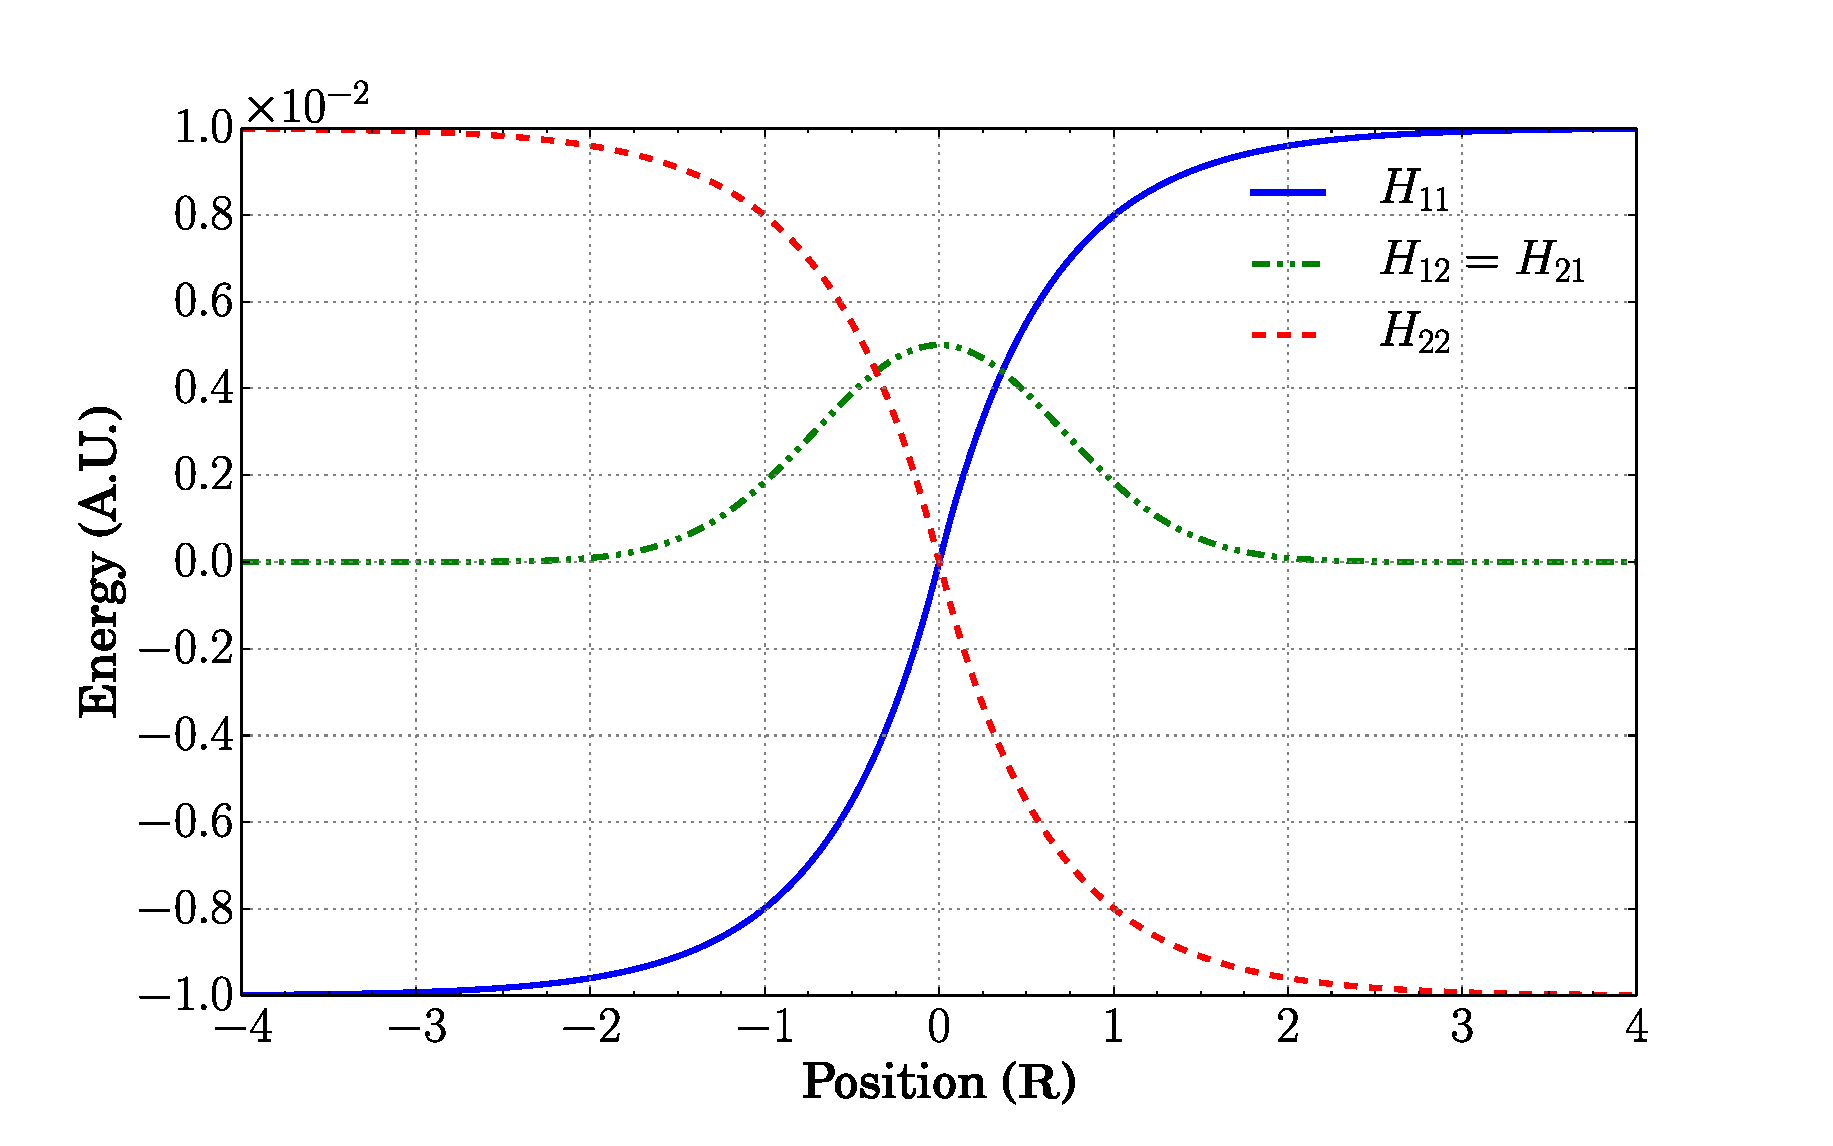
\includegraphics[scale=0.5]{scpes.eps}
\caption[Single avoided crossing: diabatic PES.]{Diabatic PES.}
\label{f:pessc}
\end{figure}

The equations of motion (\cref{eq:diab_motion}) require the calculation of 
gradients for all relevant PES. For our purposes, they can be obtained 
analytically \cref{eq:dscpes}, reducing computational demands. Less ideal 
systems would require numerical differentiation. The diabatic PES derivatives 
are:
\begin{subequations}\label{eq:dscpes}
\begin{align}
\dpar{H_{11}}{R} & = 
A B \begin{cases}
e^{-B R} &\qquad R \geq 0\\
e^{B R} &\qquad R < 0
\end{cases}
\\
\dpar{H_{22}}{R} &= -\dpar{H_{11}}{R}\\
\dpar{H_{12}}{R} &= \dpar{H_{21}}{R} = -2 C D e^{-D R^{2}} R~.
\end{align}
\end{subequations}
They are shown in \cref{f:dpessc}.

\begin{figure}
\centering
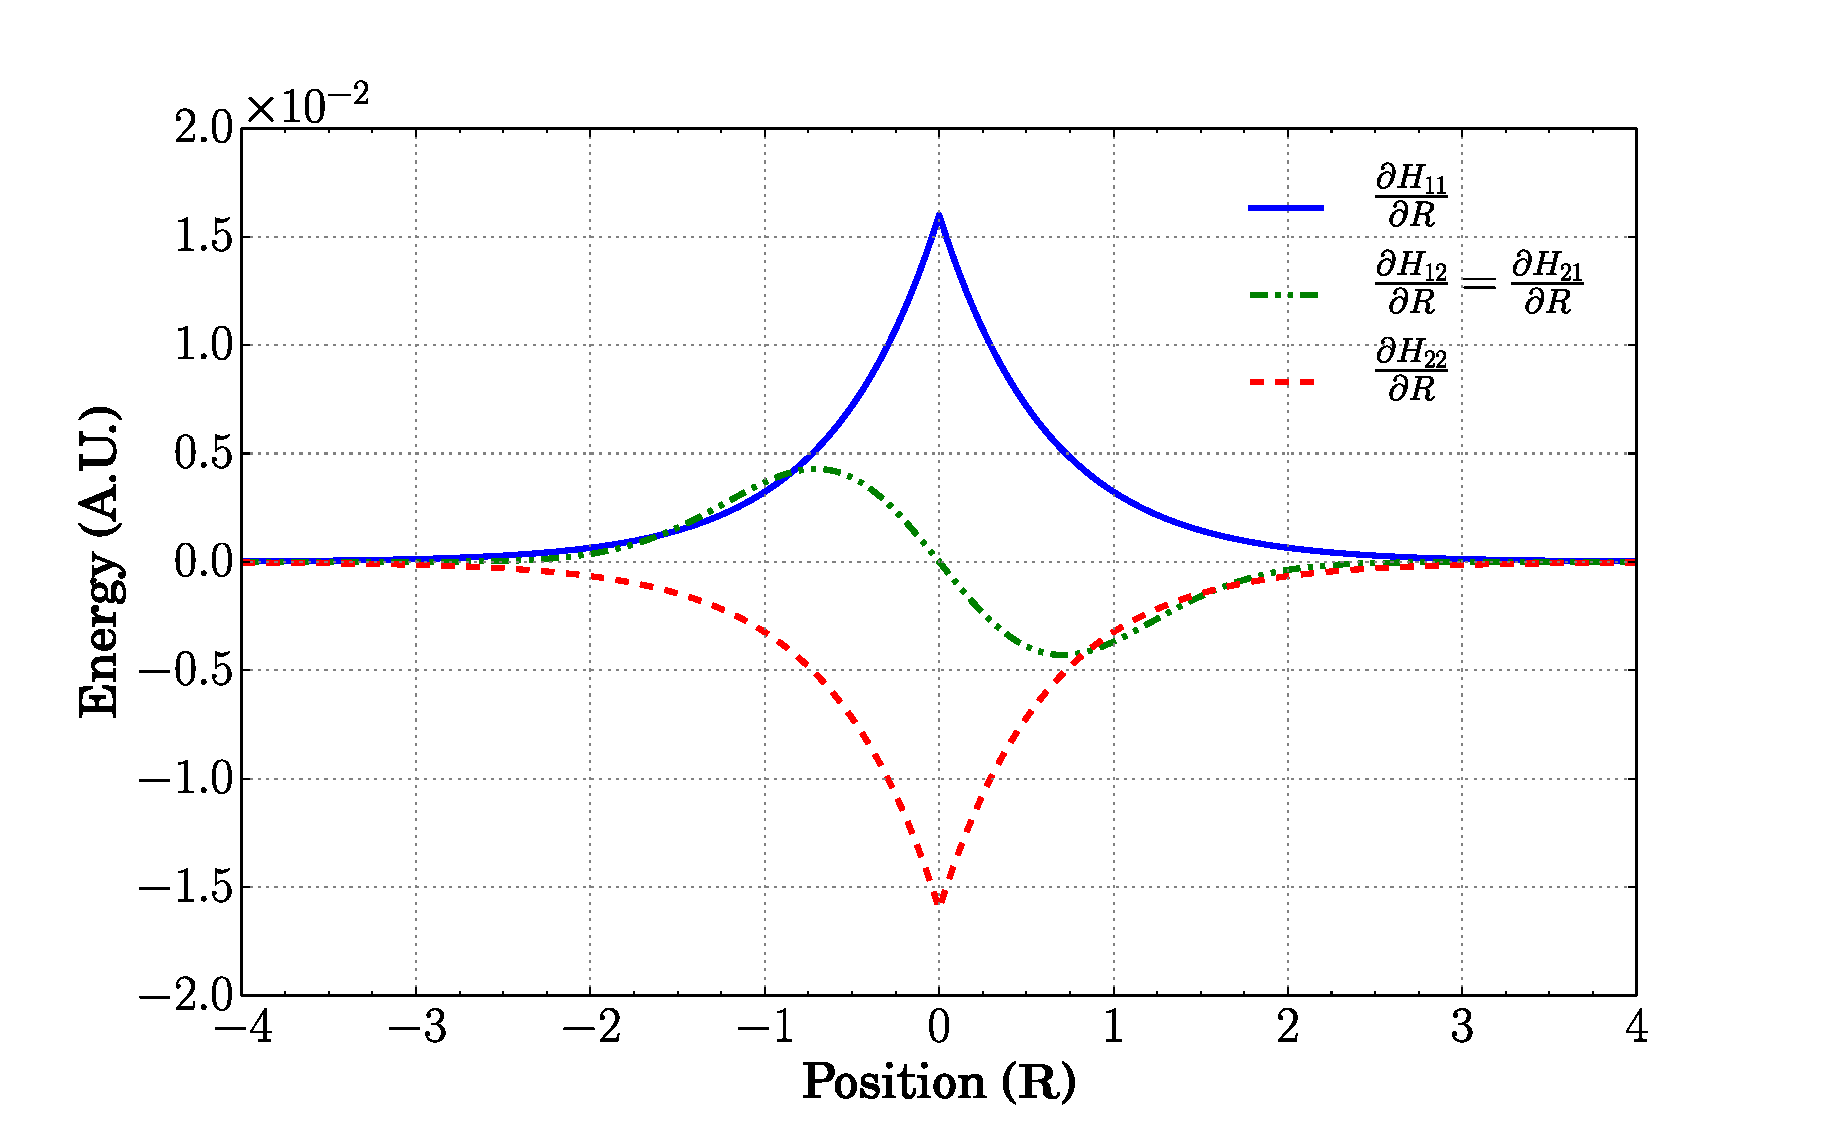
\includegraphics[scale=0.5]{dscpes.eps}
\caption[Single avoided crossing: diabatic PES derivatives.]{Diabatic PES derivatives.}
\label{f:dpessc}
\end{figure}

The adiabatic PES ($ E_{i} $) are the eigenvalues of the diabatic PES 
Hamiltonian matrix, which are obtained through eigenvalue decomposition. In our 
case, they can be obtained analytically, but less ideal systems require 
numerical methods. For the single avoided crossing, these are,
\begin{subequations}\label{eq:ascpes}
\begin{align}
E_{1} &= -e^{-D R^{2}}
\sqrt{
C^{2} + A^{2}e^{2 D R^{2}}
\begin{cases}
\left(1 - e^{-B R}\right)^{2} &\qquad R\geq 0\\
\left(1 - e^{B R}\right)^{2} &\qquad R<0
\end{cases}
}\\
E_{2} & = -E_{1}~.
\end{align}
\end{subequations}
The diabatic Hamiltonian \cref{eq:def_diab_ham} does not require the 
calculation of adiabatic PES, or their derivatives. However, it is often useful 
to visualise the adiabatic PES because they can provide us with useful physical 
insight. They are shown in \cref{f:apessc}. Their derivatives are not shown here because they are irrelevant.

\begin{figure}
\centering
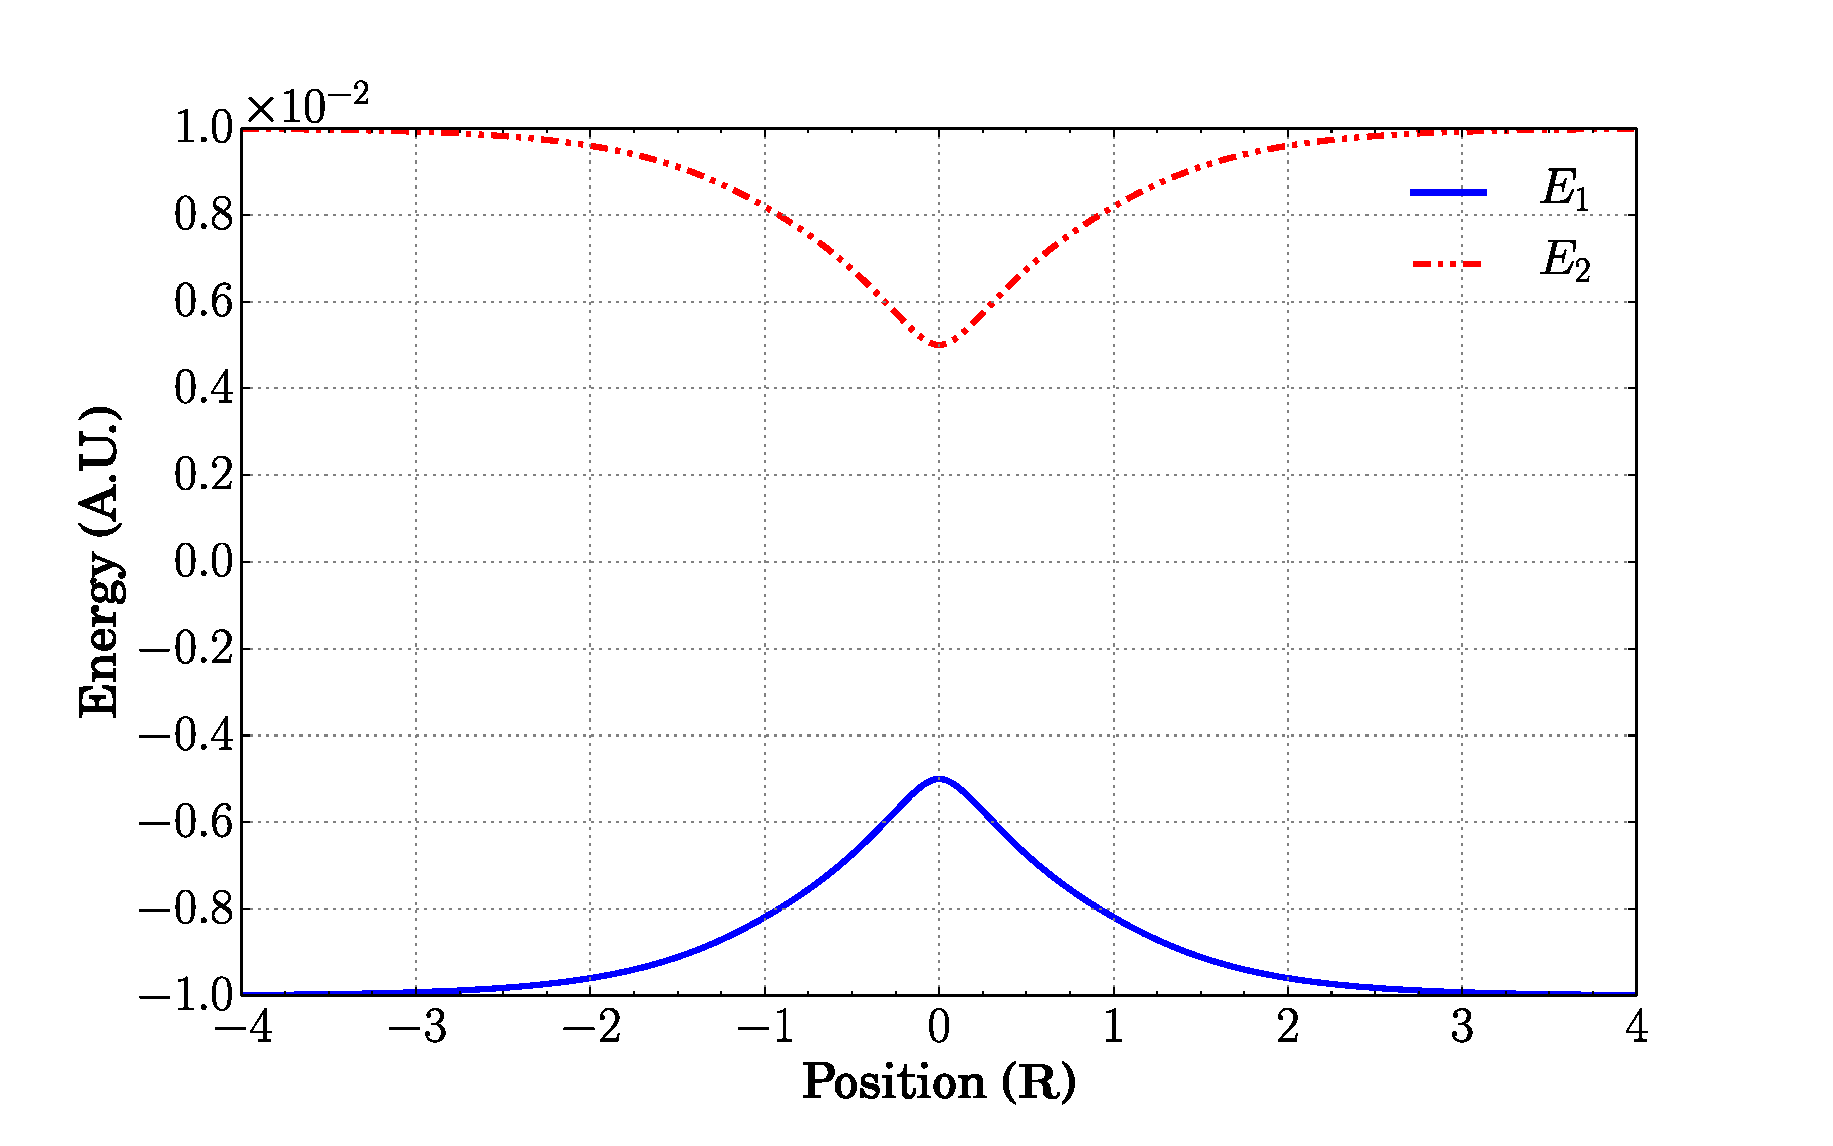
\includegraphics[scale=0.5]{ascpes.eps}
\caption[Single avoided crossing: adiabatic PES.]{Adiabatic PES. Eigenvalues of the diabatic Hamiltonian matrix.}
\label{f:apessc}
\end{figure}

The coupling between electronic states---and therefore the probability of transition---is at its greatest where there the energy difference between both adiabatic PES is at a minimum, as shown in \cref{f:delapessc}.

\begin{figure}
\centering
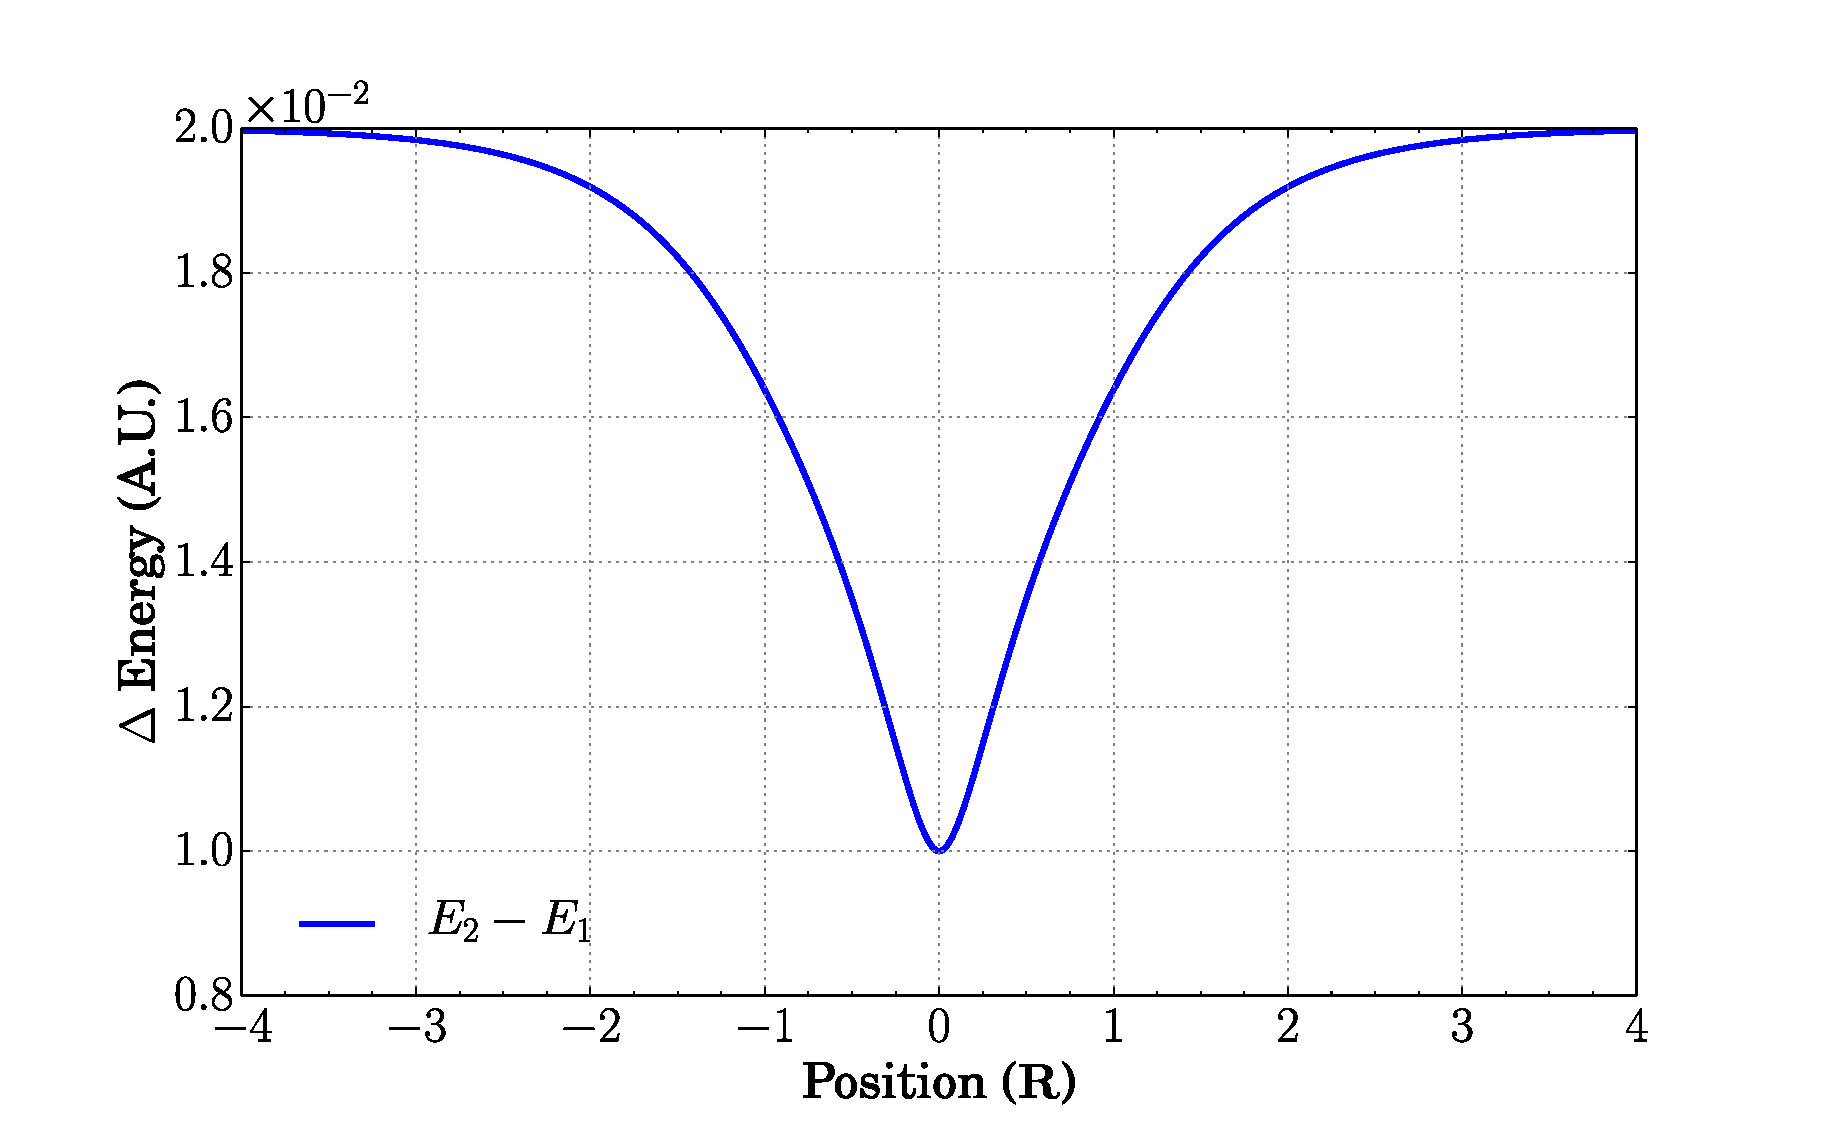
\includegraphics[scale=0.5]{del_ascpes.eps}
\caption[Single avoided crossing: energy difference between adiabatic PES.]{Energy difference between adiabatic PES.}
\label{f:delapessc}
\end{figure}
%
\subsubsection{Equations of Motion}
%
For the single avoided crossing, the equations of motion are:
\begin{subequations}
\begin{align}
\dot{R} & = \frac{P}{\mu}\\
\dot{P} & = 2 C D R e^{-D R^2} (p_{1} p_{2}+ x_{1} x_{2})-\frac{1}{2} \left(p_{1}^{2} + x_{1}^{2} - p_{2}^{2} - x_{2}^{2}\right)
A B \begin{cases}
e^{-B R} &\quad R \geq 0\\
e^{B R} &\quad R < 0
\end{cases}\\
\dot{x}_{1} & = C p_2 e^{-D R^2}+p_1
A \begin{cases}
(1 - e^{-B R}) &\quad R \geq 0\\
(e^{B R} - 1) &\quad R < 0
\end{cases}\\
\dot{p}_{1} & = -C x_2 e^{-D R^2}-x_1
A \begin{cases}
(1 - e^{-B R}) &\quad R \geq 0\\
(e^{B R} - 1) &\quad R < 0
\end{cases}\\
\dot{x}_{2} & = C p_1 e^{-D R^2}-p_2
A \begin{cases}
(1 - e^{-B R}) &\quad R \geq 0\\
(e^{B R} - 1) &\quad R < 0
\end{cases}\\
\dot{p}_{2} & = -C x_1 e^{-D R^2} + x_2
A \begin{cases}
(1 - e^{-B R}) &\quad R \geq 0\\
(e^{B R} - 1) &\quad R < 0
\end{cases}~.
\end{align}
\end{subequations}
%
\subsection{Double Avoided Crossing}\label{s:dac}
%
\subsubsection{Potential Energy Surfaces}
%
The diabatic PES for the double avoided crossing were defined by Tully \cite{tully} as:
\begin{subequations}
\begin{align}
H_{11}(R) &= 0 \\
H_{22}(R) &= -A e^{-B R^{2}} + E_{0}\\
H_{12}(R) &= H_{21}(R) = C e^{-D R^{2}}~,
\end{align}
\end{subequations}
where $ A = 0.1,~B = 0.28,~C = 0.015,~D = 0.06,~\text{and}~E_{0} = 0.05$. They are shown in \cref{f:pesdc}.

\begin{figure}
\centering
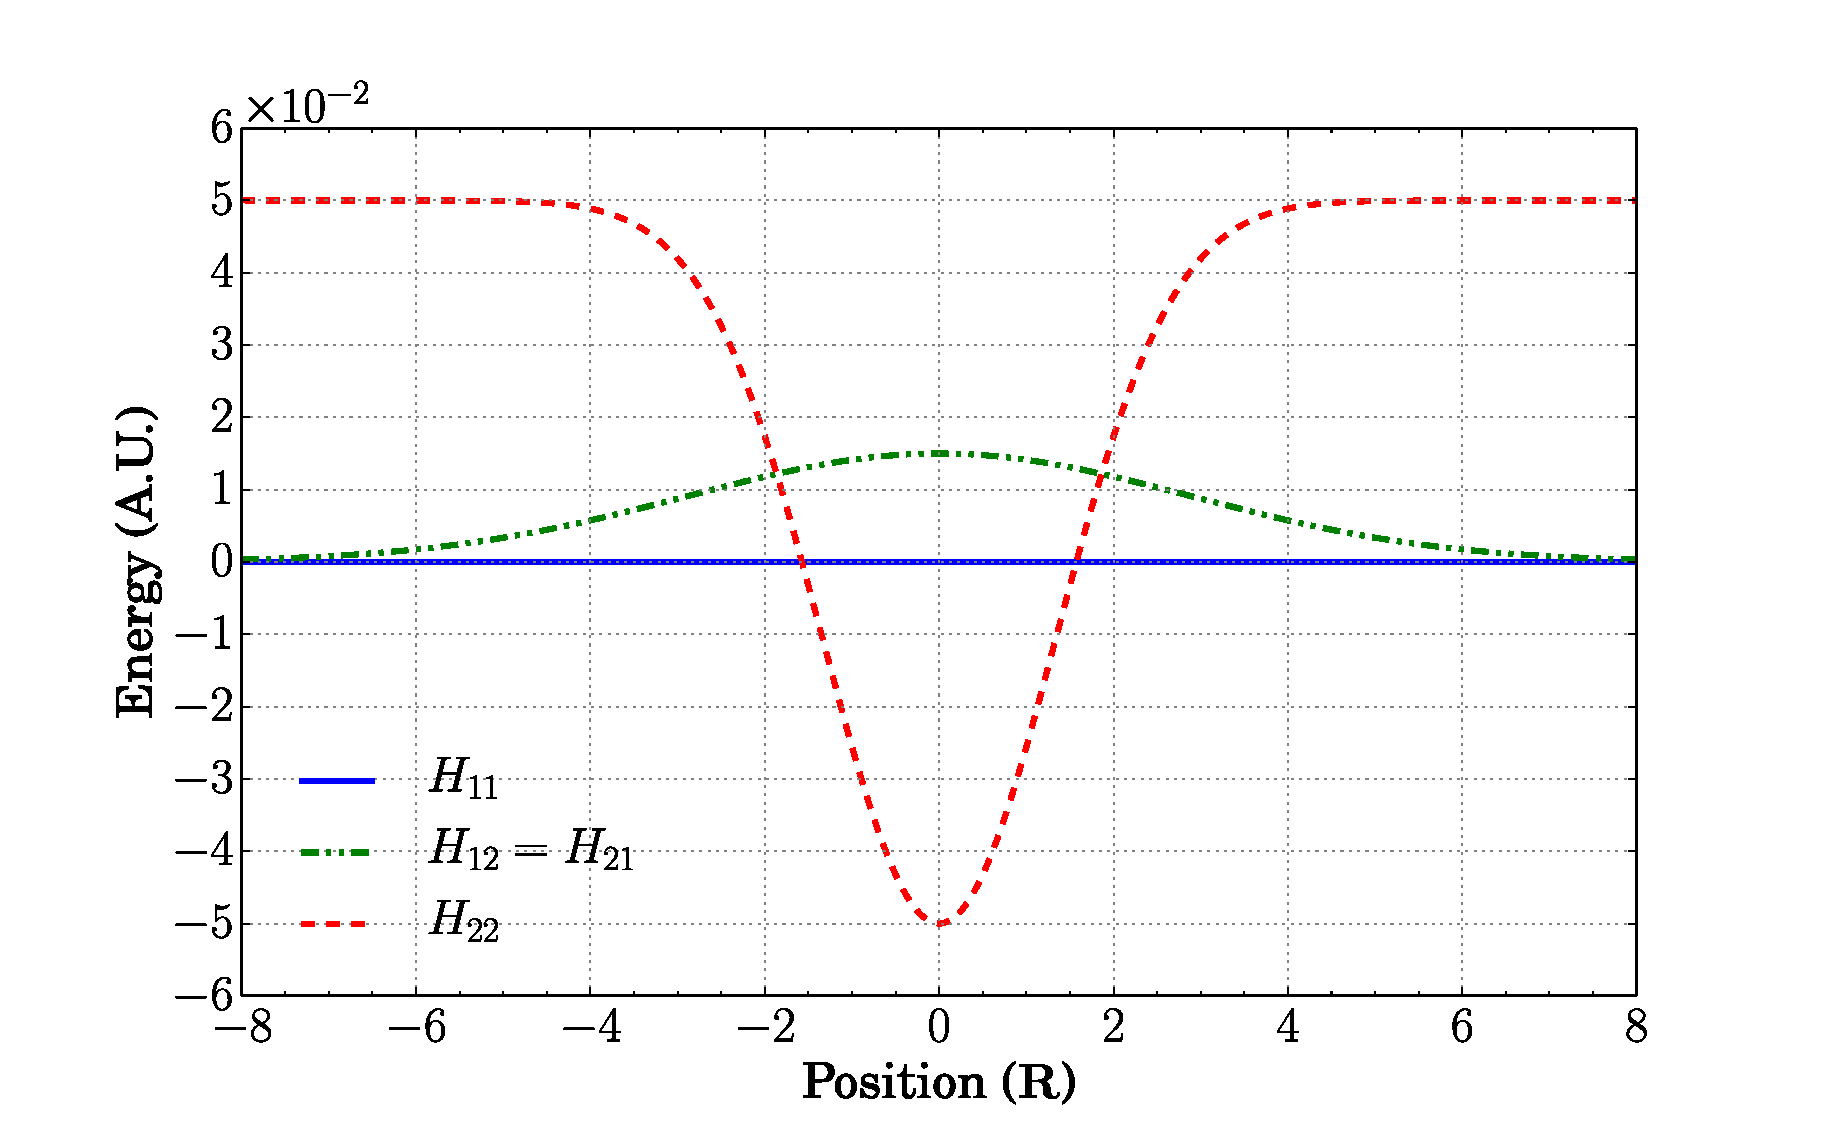
\includegraphics[scale=0.5]{dcpes.eps}
\caption[Double avoided crossing: diabatic PES.]{Diabatic PES.}
\label{f:pesdc}
\end{figure}

Their derivatives are:
\begin{subequations}
\begin{align}
\dpar{H_{11}}{R} &= 0\\
\dpar{H_{22}}{R} &= 2 A B e^{-B R^{2}} R\\
\dpar{H_{12}}{R} &= \dpar{H_{21}}{R} = -2 C D e^{-D R^{2}} R~.
\end{align}
\end{subequations}
They are shown in \cref{f:dpesdc}.

\begin{figure}
\centering
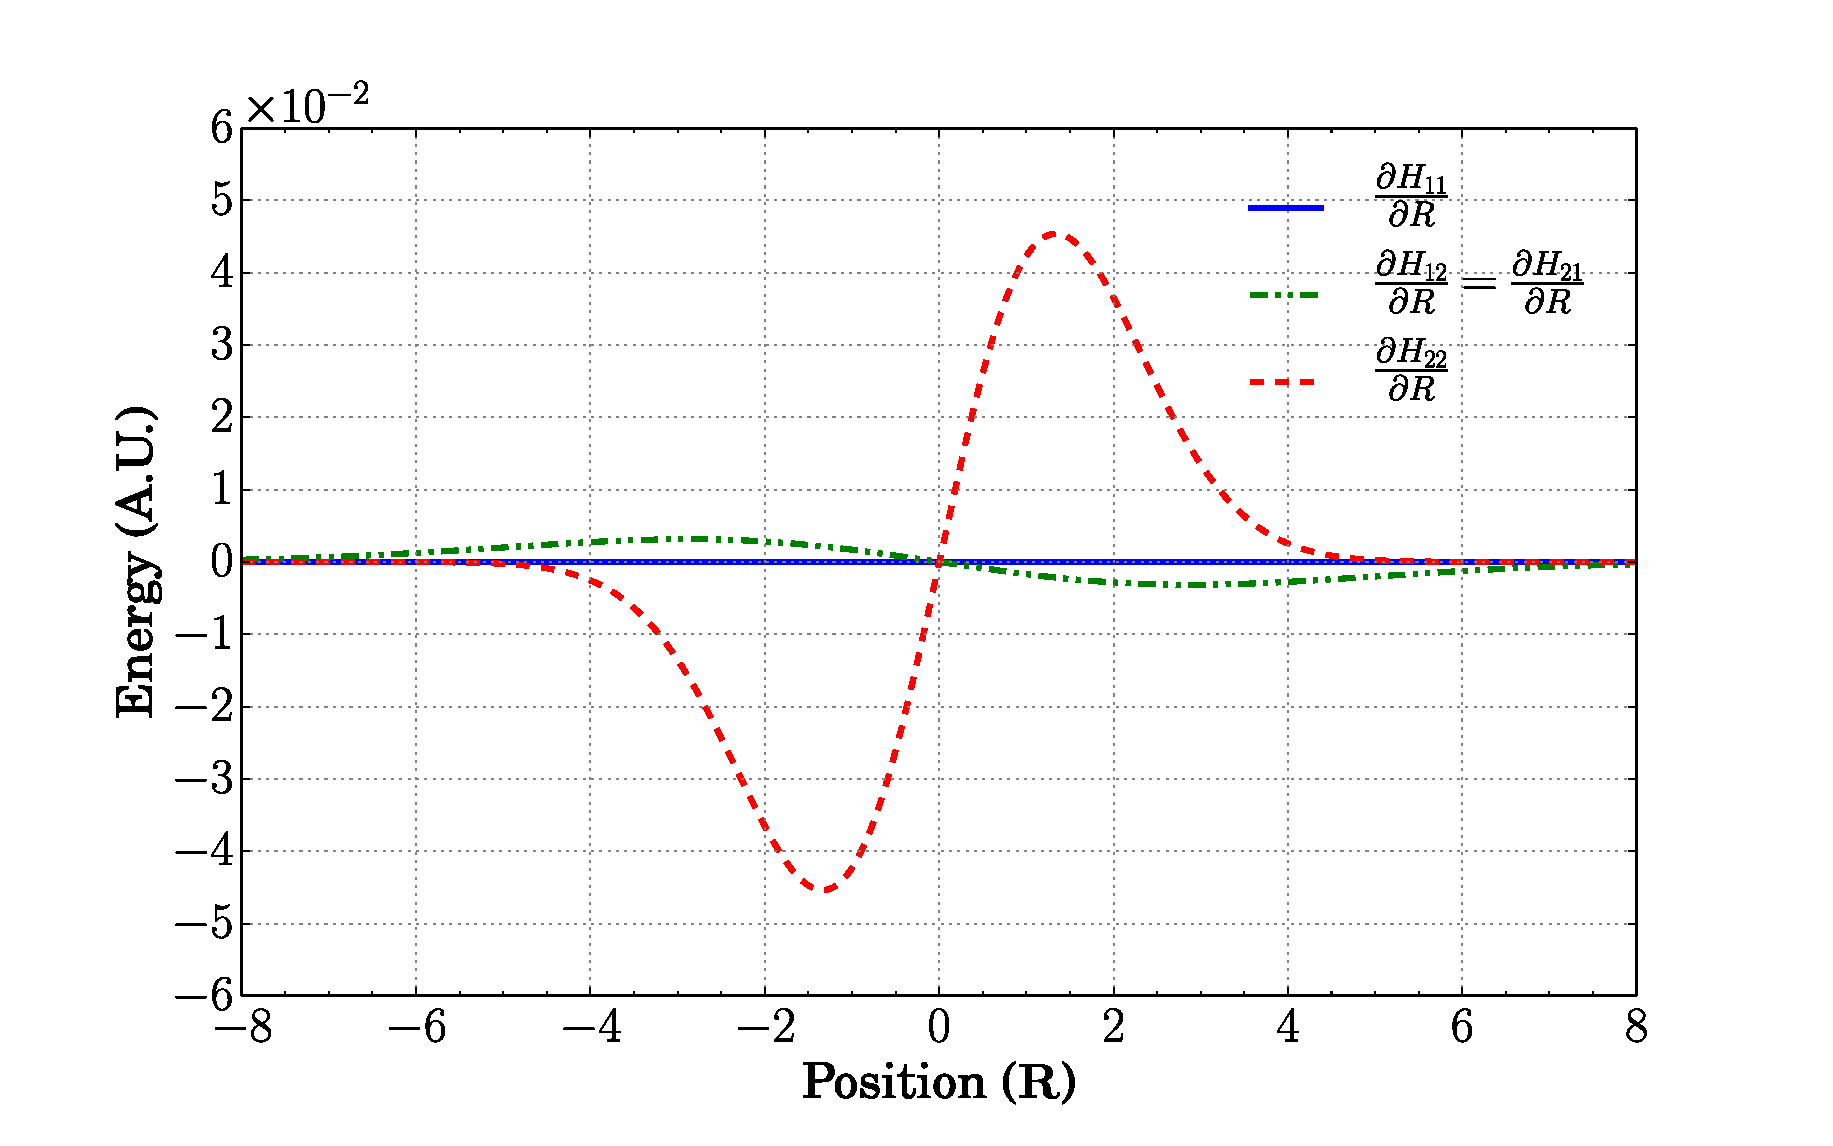
\includegraphics[scale=0.5]{ddcpes.eps}
\caption[Double avoided crossing: diabatic PES derivatives.]{Diabatic PES derivatives.}
\label{f:dpesdc}
\end{figure}

The adiabatic PES are:
\begin{subequations}
\begin{align}
E_{1} &= \frac{1}{2} e^{-(B+D) R^{2}}
\left(
-A e^{D R^{2}} + e^{(B+D) R^{2}} E_{0} -
\sqrt{
4 C^{2} e^{2 B R^{2}} + e^{2 D R^{2}}\left( A - e^{B R^{2}} E_{0} \right)^{2}
}
\right)\\
E_{2} &= \frac{1}{2} e^{-(B+D) R^{2}}
\left(
-A e^{D R^{2}} + e^{(B+D) R^{2}} E_{0} +
\sqrt{
4 C^{2} e^{2 B R^{2}} + e^{2 D R^{2}}\left( A - e^{B R^{2}} E_{0} \right)^{2}
}
\right)~.
\end{align}
\end{subequations}
They are shown in \cref{f:apesdc}

\begin{figure}
\centering
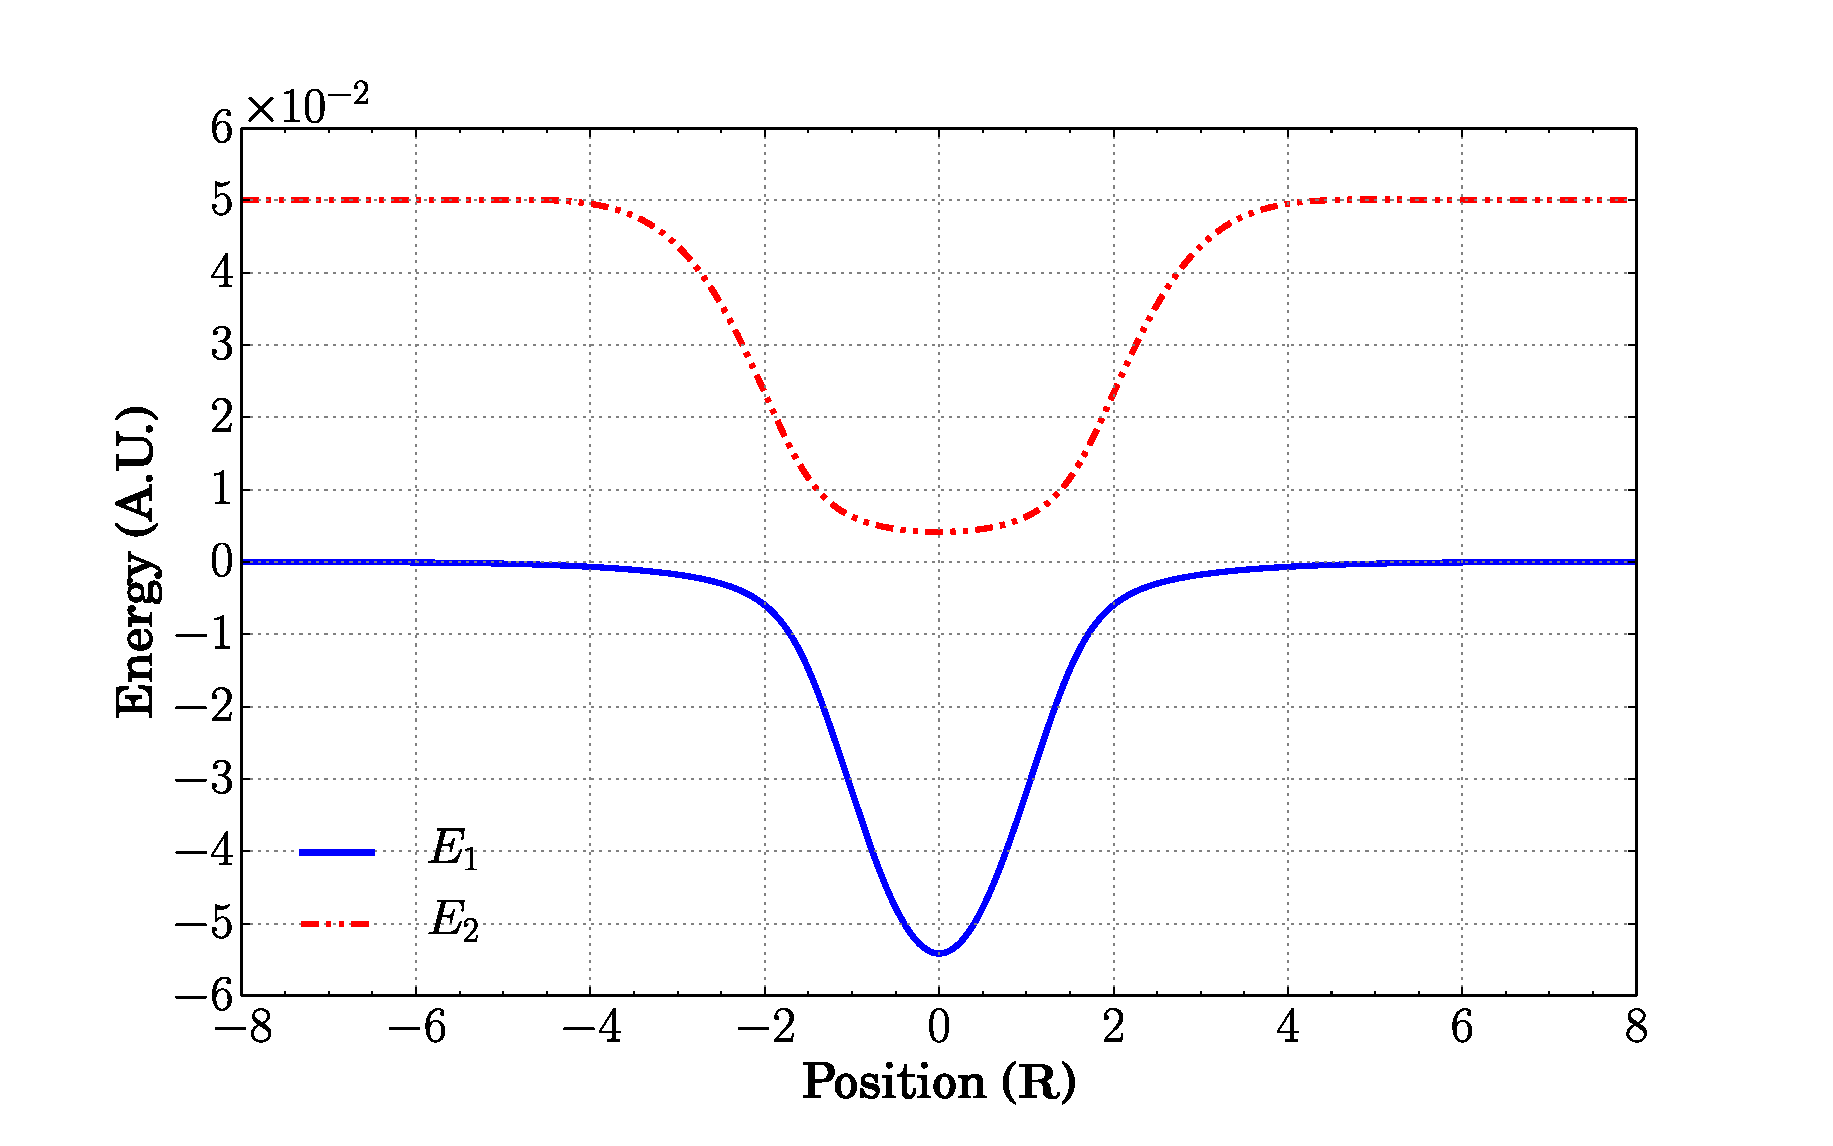
\includegraphics[scale=0.5]{adcpes.eps}
\caption[Double avoided crossing: adiabatic PES.]{Adiabatic PES. Eigenvalues of the diabatic Hamiltonian matrix.}
\label{f:apesdc}
\end{figure}

In this case, there are two minimum energy gaps between both adiabatic PES, shown in \cref{f:delapesdc}. This brings about some rather interesting behaviours shown in \cref{s:rdac}.

\begin{figure}
\centering
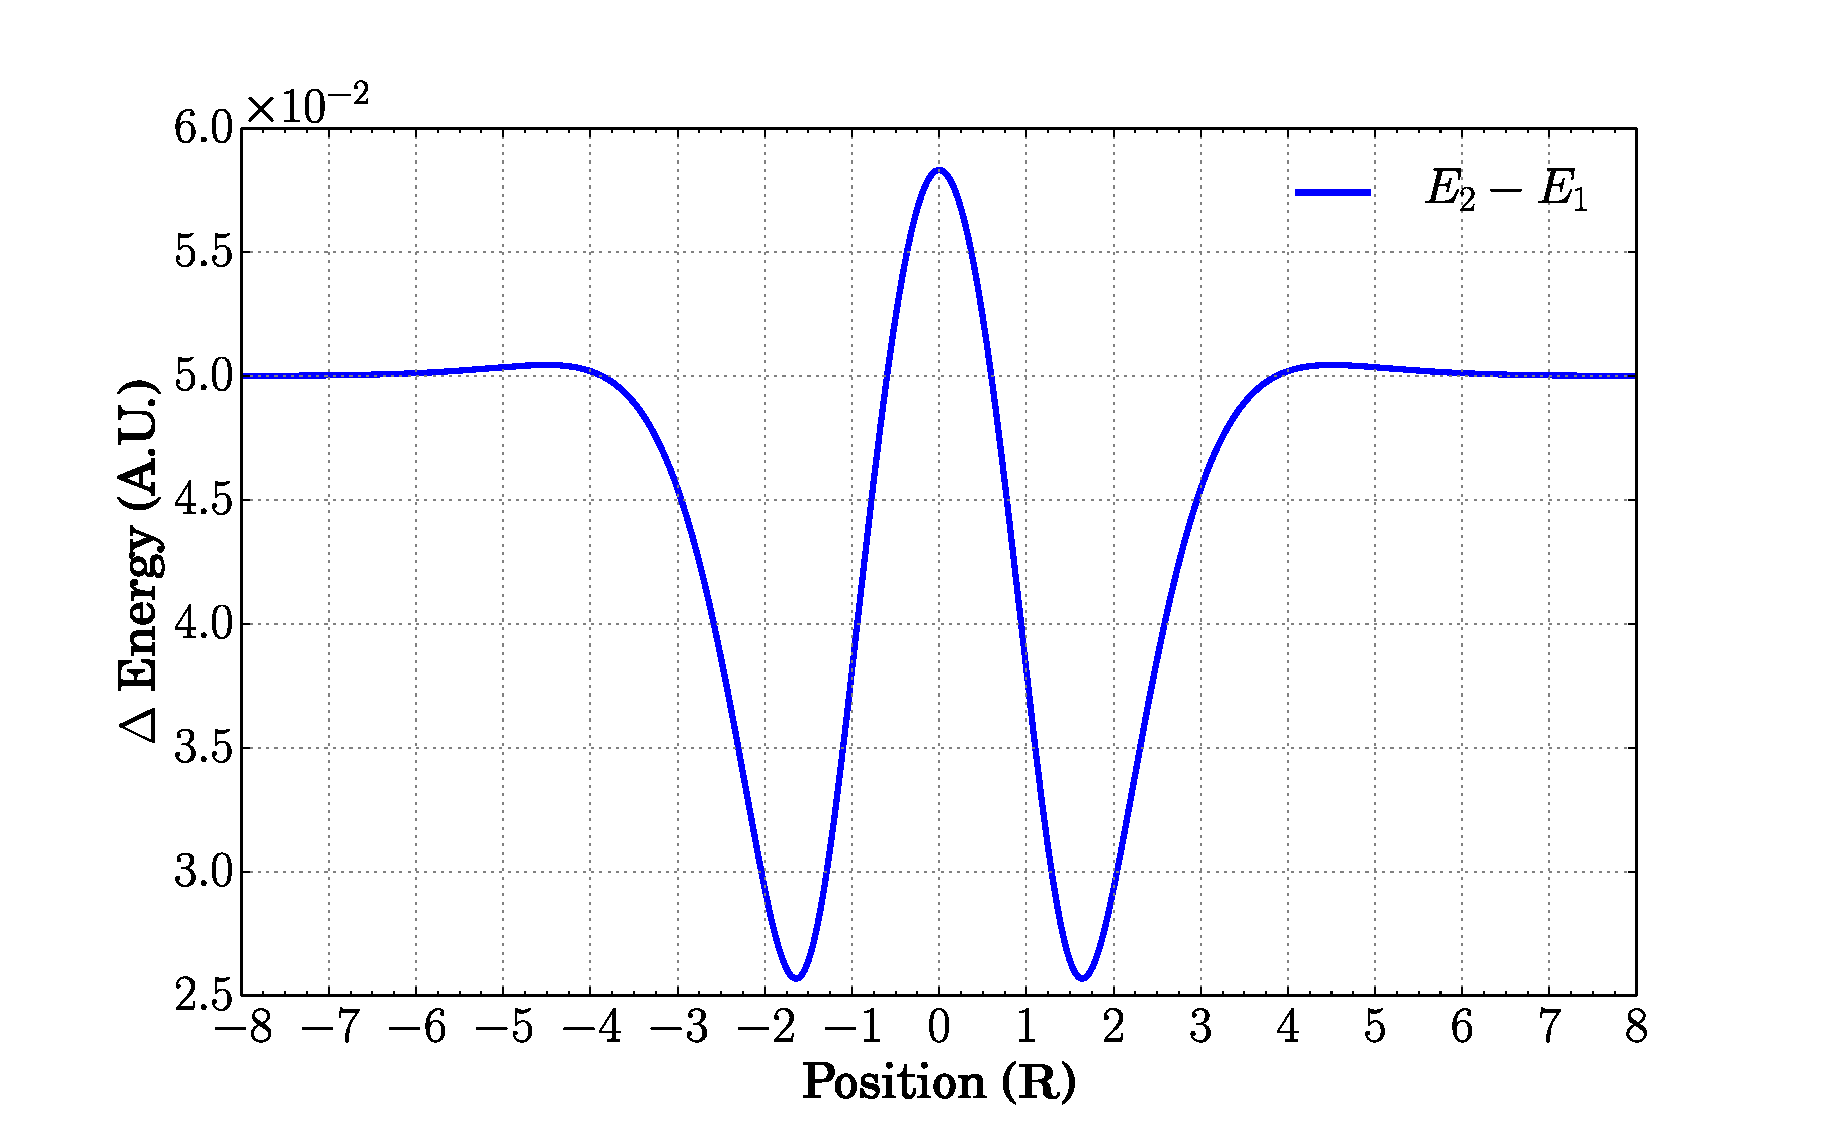
\includegraphics[scale=0.5]{del_adcpes.eps}
\caption[Double avoided crossing: energy difference between adiabatic PES.]{Energy difference between adiabatic PES.}
\label{f:delapesdc}
\end{figure}
%
\subsubsection{Equations of Motion}
%
For the double avoided crossing, the equations of motion are:
\begin{subequations}
\begin{align}
\dot{R} & = \frac{P}{\mu }\\
\dot{P} & = R \left(A B e^{-B R^2} \left(\frac{p_1^2}{2}-\frac{p_2^2}{2}+\frac{x_1^2}{2}-\frac{x_2^2}{2}-1\right)+2 C D e^{-D R^2} (p_1 p_2+ x_1 x_2)\right)\\
\dot{x}_{1} & = \frac{1}{2} p_1 \left(A e^{-B R^2}-E_0\right)+C p_2 e^{-D R^2}\\
\dot{p}_{1} & = -\frac{1}{2} x_1 \left(A e^{-B R^2}-E_0\right)-C x_2 e^{-D R^2}\\
\dot{x}_{2} & = -\frac{1}{2} p_2 \left(A e^{-B R^2}-E_0\right) + C p_1 e^{-D R^2}\\
\dot{p}_{2} & = \frac{1}{2} x_2 \left(A e^{-B R^2}-E_0\right)-C x_1 e^{-D R^2}~.
\end{align}
\end{subequations}
%
\subsection{Extended Coupling}\label{s:ec}
%
\subsubsection{Potential Energy Surfaces}
%
This problem has non-vanishing non-diagonal elements in the Hamiltonian matrix. Said elements are perturbations from a pure state, and when they do not vanish as $ R \rightarrow \pm\infty $, one must use the adiabatic Hamiltonian. The diagonal elements of the Hamiltonian matrix are also constant, lending further arguments to the use of the adiabatic Hamiltonian due to the system's relatively unchanging conditions.

The diabatic PES for the extended coupling problem were defined by Tully \cite{tully} as:
\begin{subequations}
\begin{align}
H_{11}(R) & = -A\\
H_{22}(R) & = -H_{11}\\
H_{12}(R) & = H_{21}(R) = 
B\begin{cases}
\left(2 - e^{-C R}\right) &\qquad R \geq 0 \\
e^{C R} &\qquad R<0
\end{cases}~,
\end{align}
\end{subequations}
where $ A = 6 \times 10^{-4},~B = 0.1,~\text{and}~C = 0.9$. They are shown in \cref{f:pesec}.

\begin{figure}
\centering
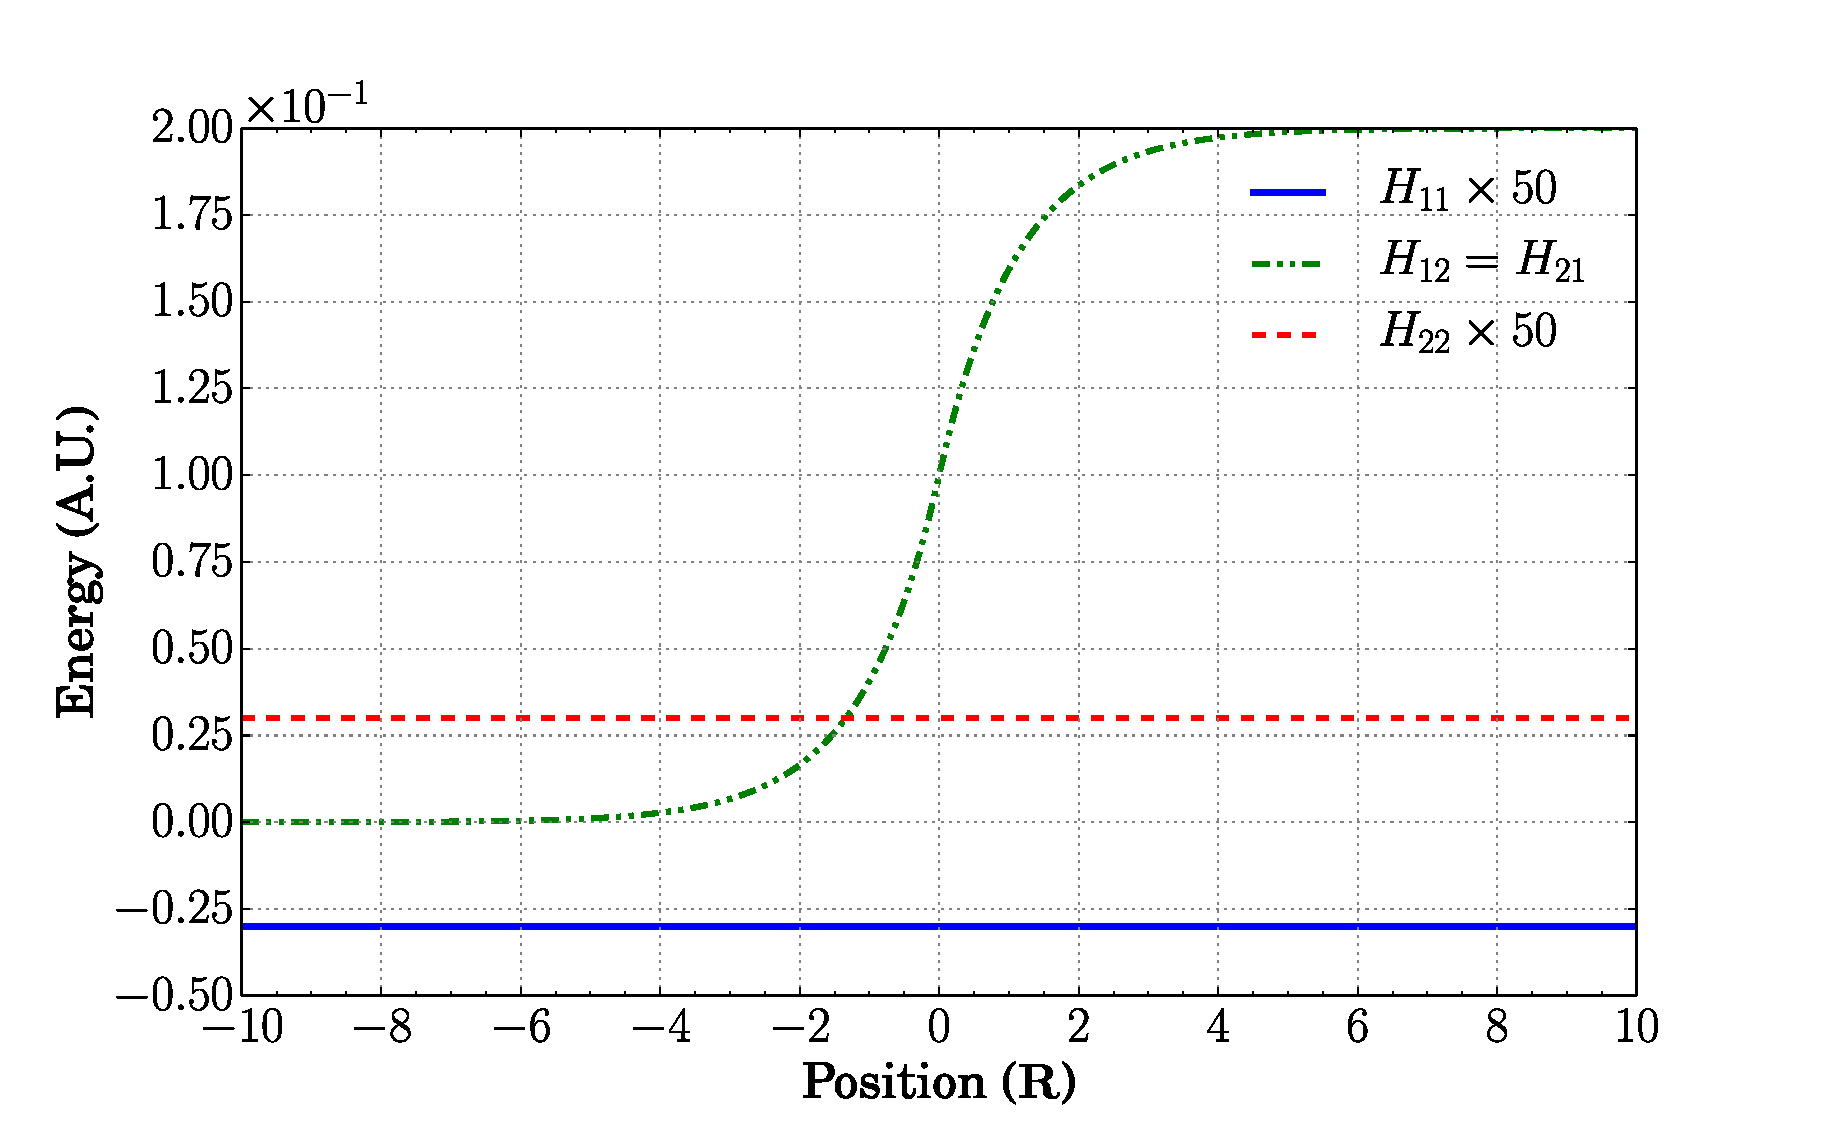
\includegraphics[scale=0.5]{ecpes.eps}
\caption[Extended coupling: diabatic PES.]{Diabatic PES.}
\label{f:pesec}
\end{figure}

The diabatic PES derivatives are:
\begin{subequations}
\begin{align}
\dpar{H_{11}}{R} &= \dpar{H_{22}}{R} = 0\\
\dpar{H_{12}}{R} &= \dpar{H_{21}}{R} = 
B C\begin{cases}
e^{-C R} &\qquad R \geq 0\\
e^{C R} &\qquad R<0~.
\end{cases}
\end{align}
\end{subequations}
They are shown in \cref{f:dpesec}.

\begin{figure}
\centering
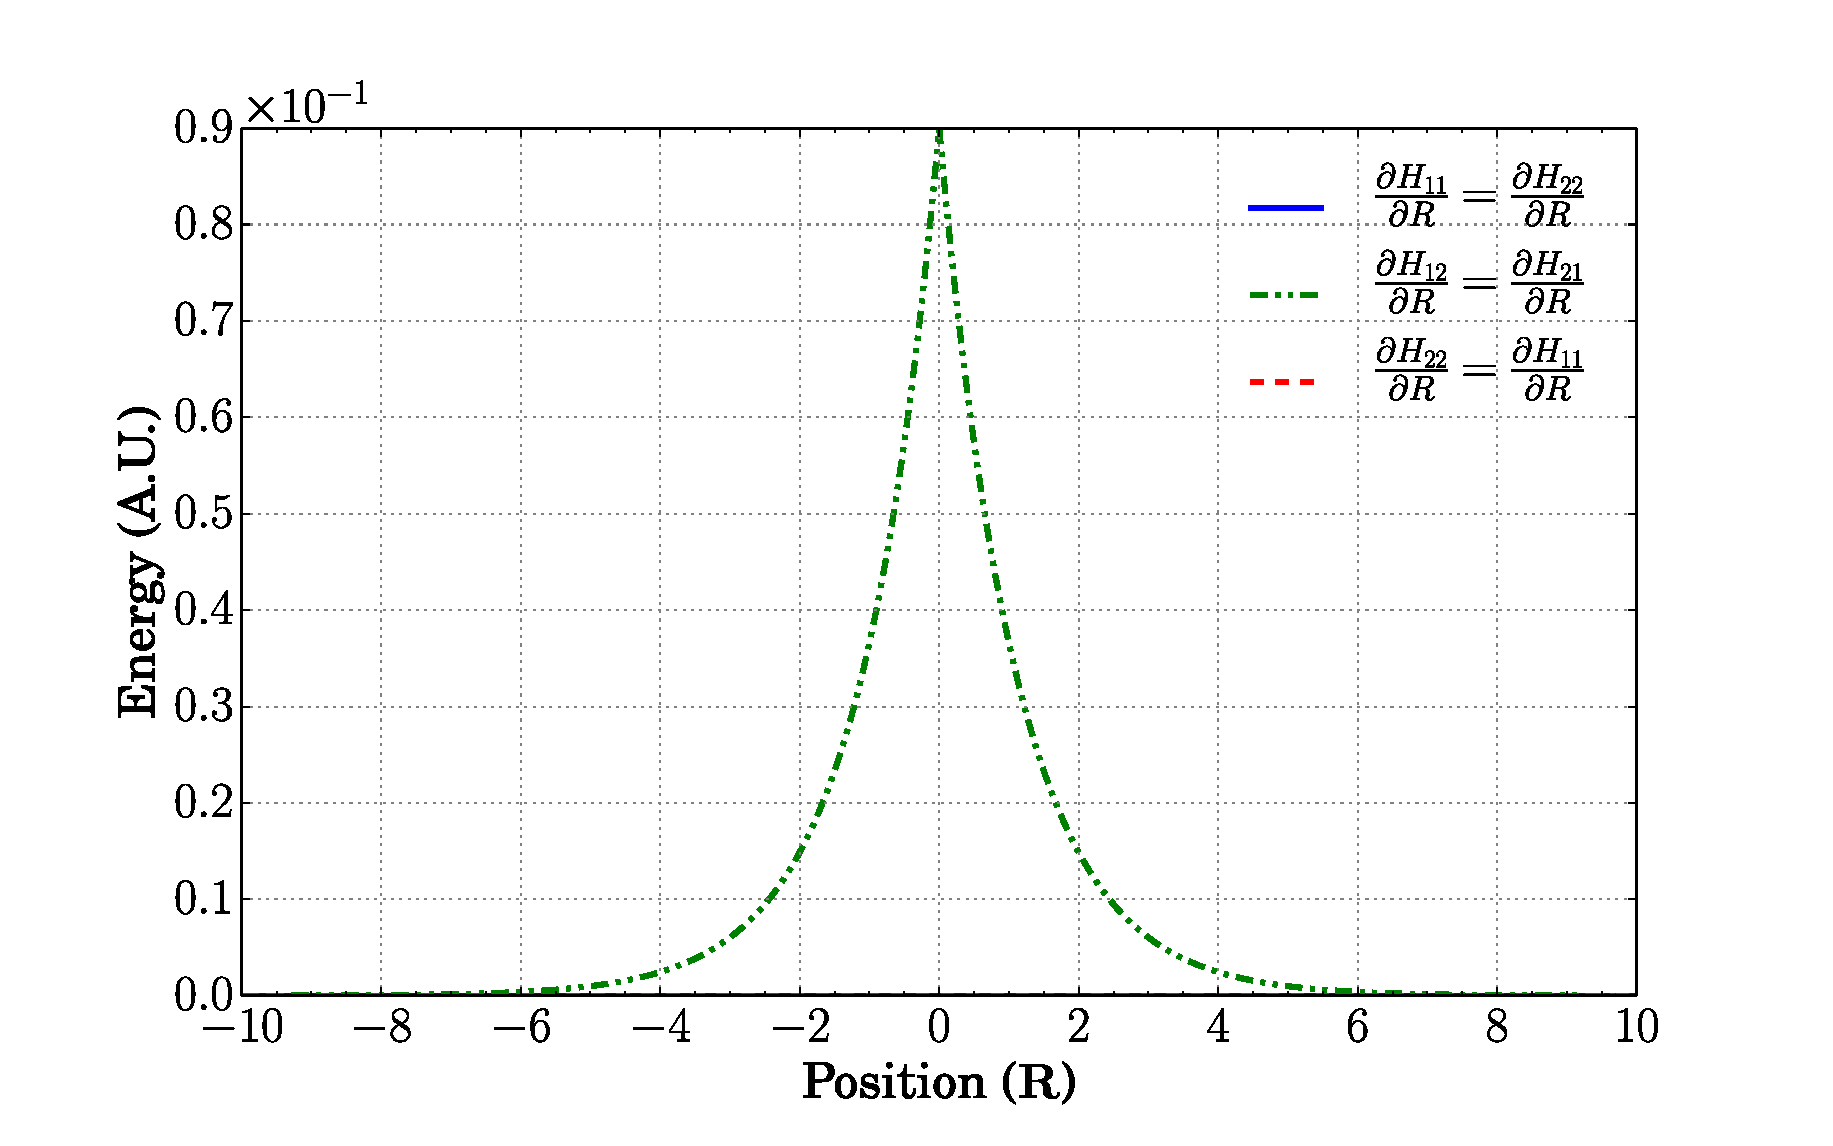
\includegraphics[scale=0.5]{decpes.eps}
\caption[Extended coupling: diabatic PES derivatives.]{Diabatic PES derivatives.}
\label{f:dpesec}
\end{figure}

The adiabatic PES are:
\begin{subequations}
\begin{align}
E_{1} & = -\sqrt{A^{2} 
+ B^{2}\begin{cases}
(2 - e^{-C R})^{2} &\qquad R \geq 0\\
e^{2C R} &\qquad R<0
\end{cases}
}\\
E_{2} &= -E_{1}~.
\end{align}
\end{subequations}
They are shown in \cref{f:apesec}.

\begin{figure}
\centering
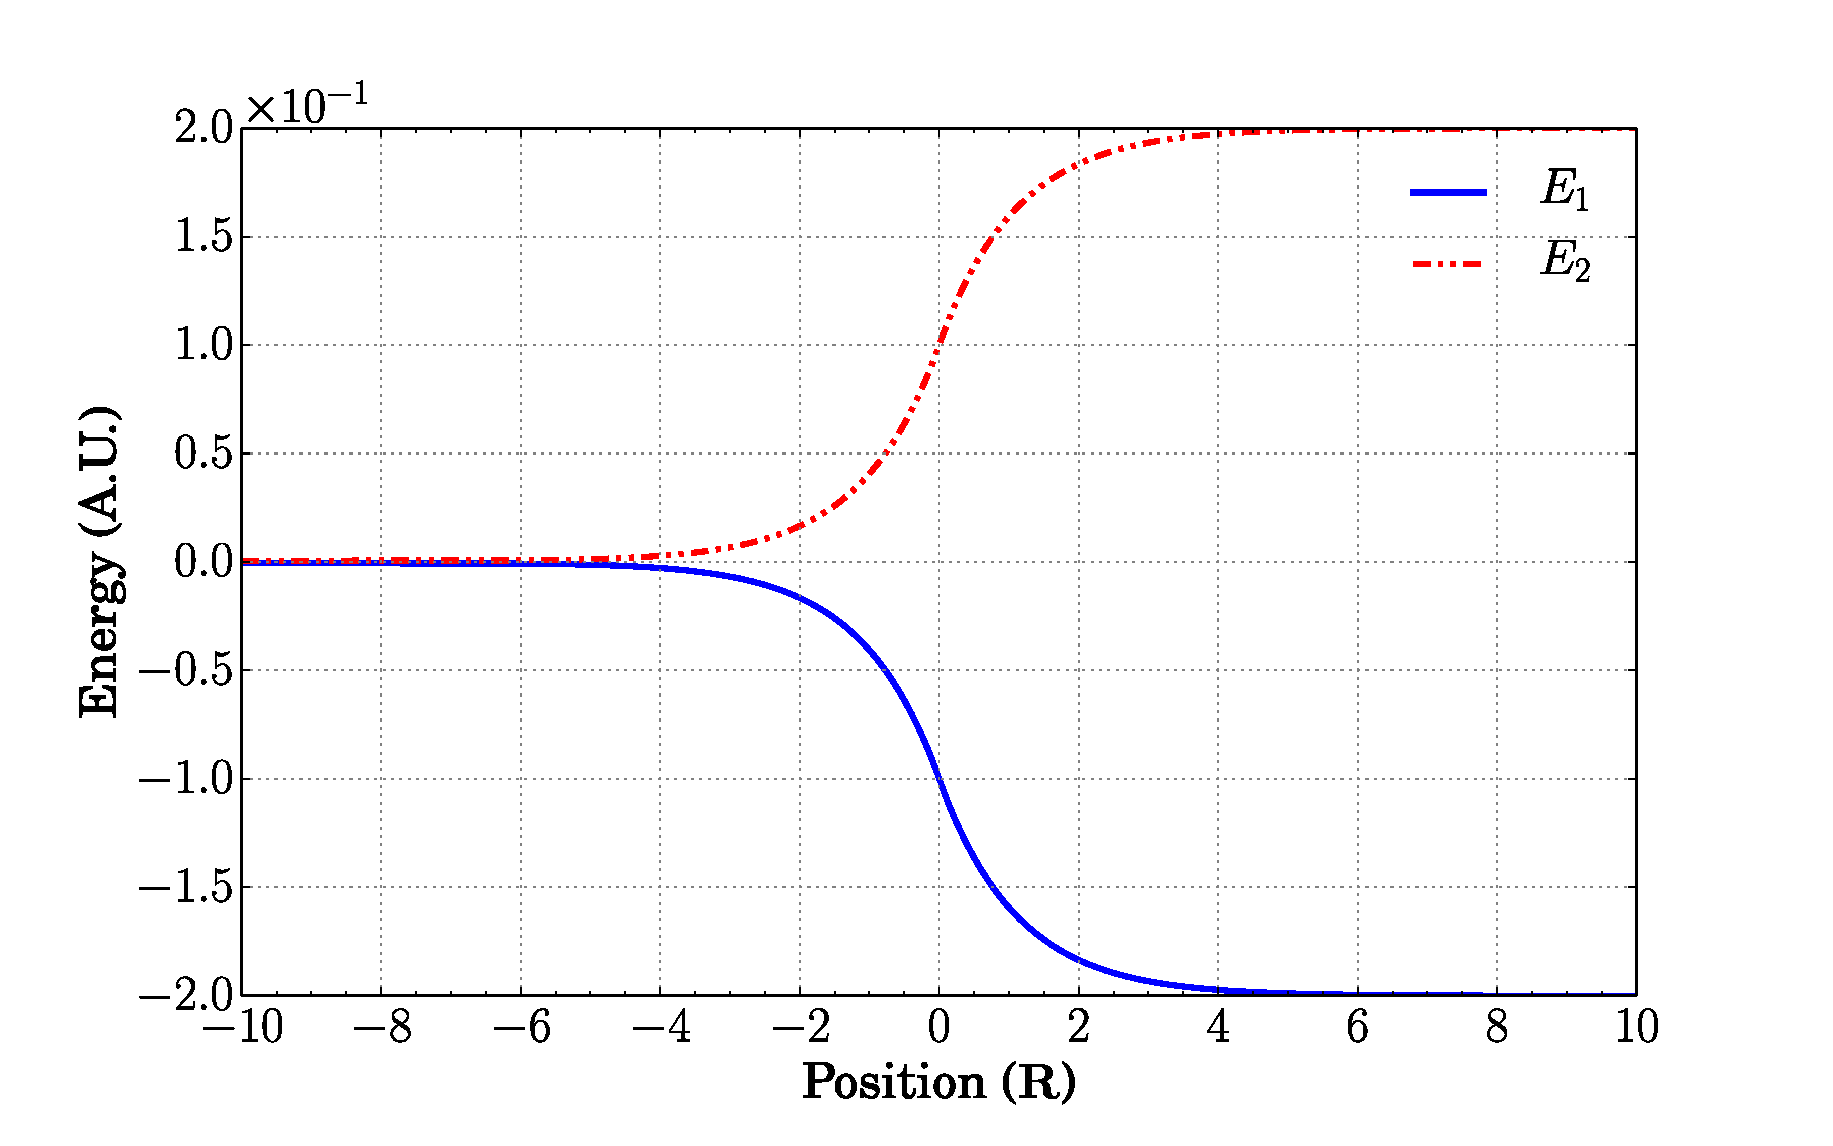
\includegraphics[scale=0.5]{aecpes.eps}
\caption[Extended coupling: adiabatic PES.]{Adiabatic PES. Eigenvalues of the diabatic Hamiltonian matrix.}
\label{f:apesec}
\end{figure}

Their derivatives are:
\begin{subequations}
\begin{align}
\dpar{E_{1}}{R} &=
\begin{cases}
-\dfrac{B^2 C e^{-2 C R} \left(2 e^{C R}-1\right)}{\sqrt{A^2+B^2 \left(e^{-C R}-2\right)^2}} & \qquad R \geq 0\\
-\dfrac{B^2 C e^{2 C R}}{\sqrt{A^2+B^2 e^{2 C R}}} &\qquad R<0
\end{cases}\\
\dpar{E_{2}}{R} &= -\dpar{E_{1}}{R}~.
\end{align}
\end{subequations}
They are shown in \cref{f:dapesec}.

\begin{figure}
\centering
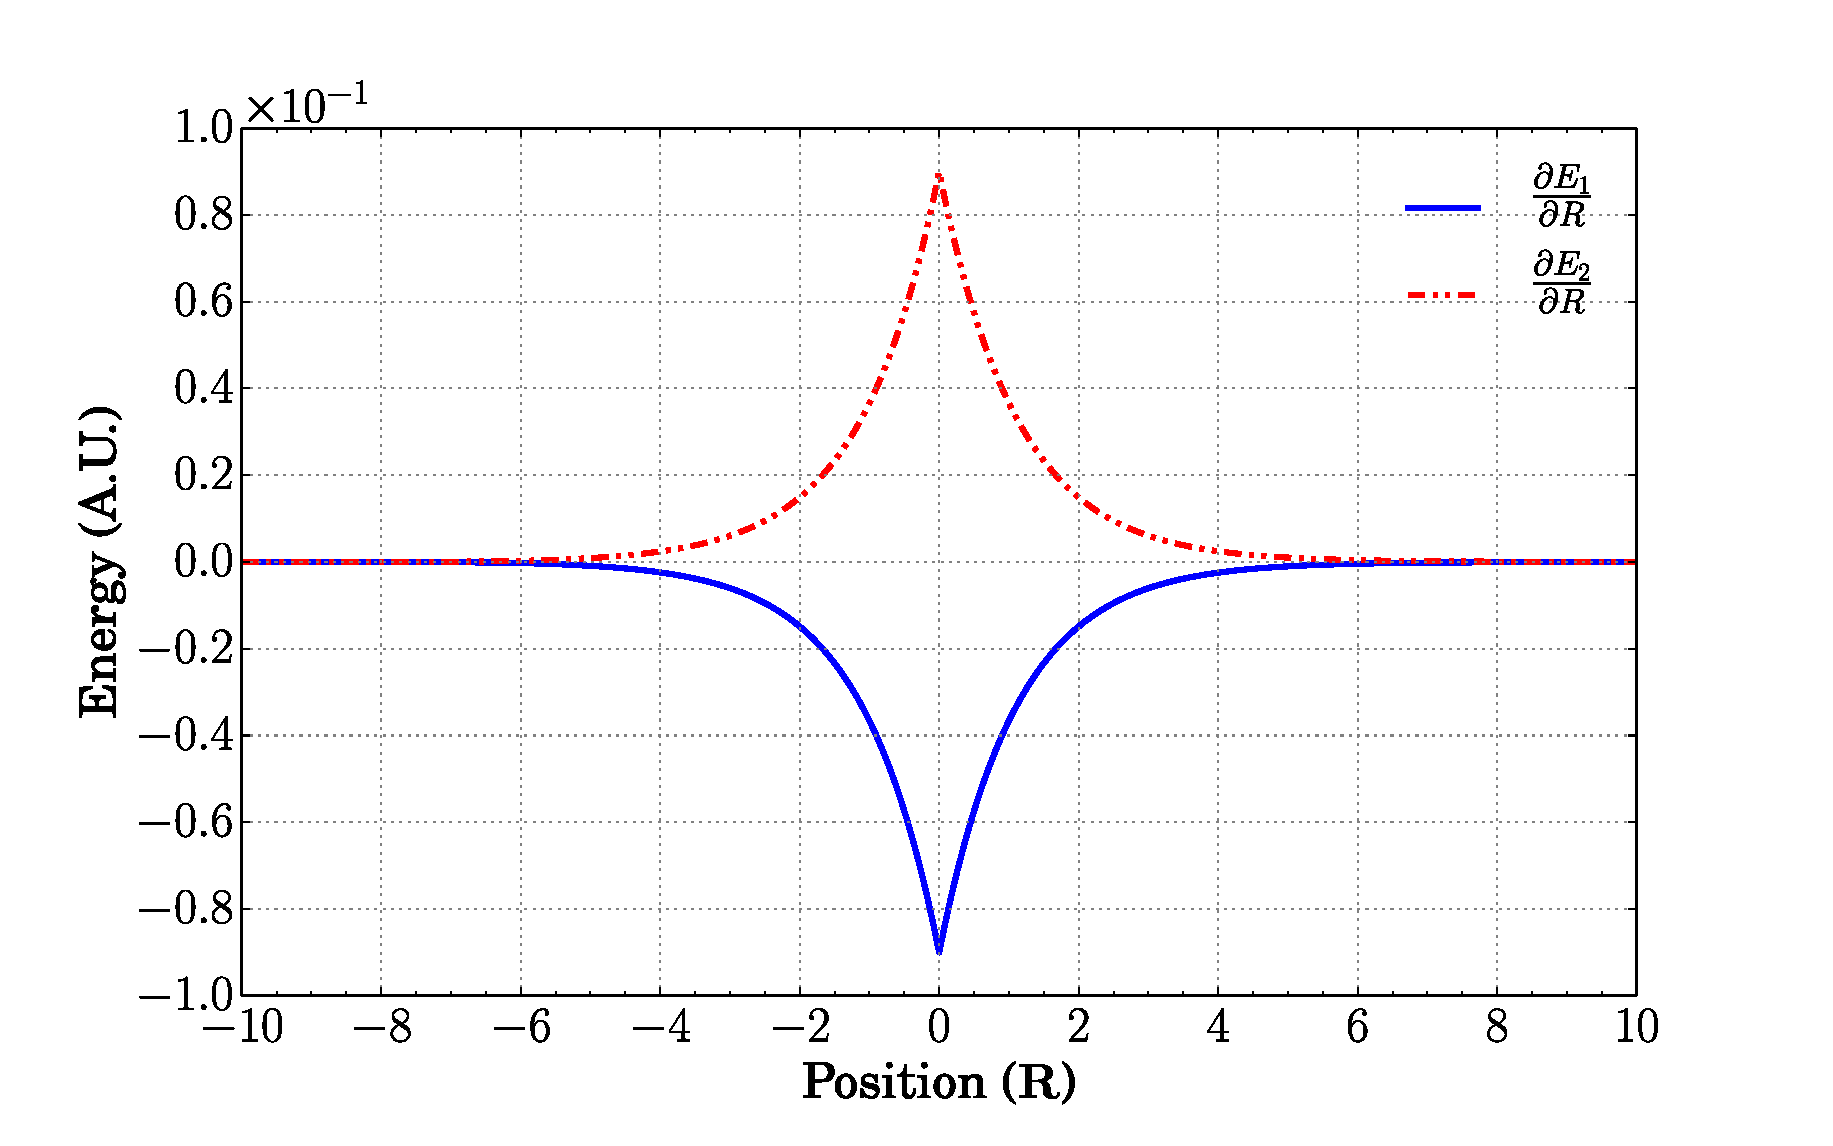
\includegraphics[scale=0.5]{daecpes.eps}
\caption[Extended coupling: adiabatic PES derivatives.]{Adiabatic PES derivatives. Derivatives of the eigenvalues of the diabatic Hamiltonian matrix.}
\label{f:dapesec}
\end{figure}

The energy difference between both adiabatic PES is shown in \cref{f:delapesec}.

\begin{figure}
\centering
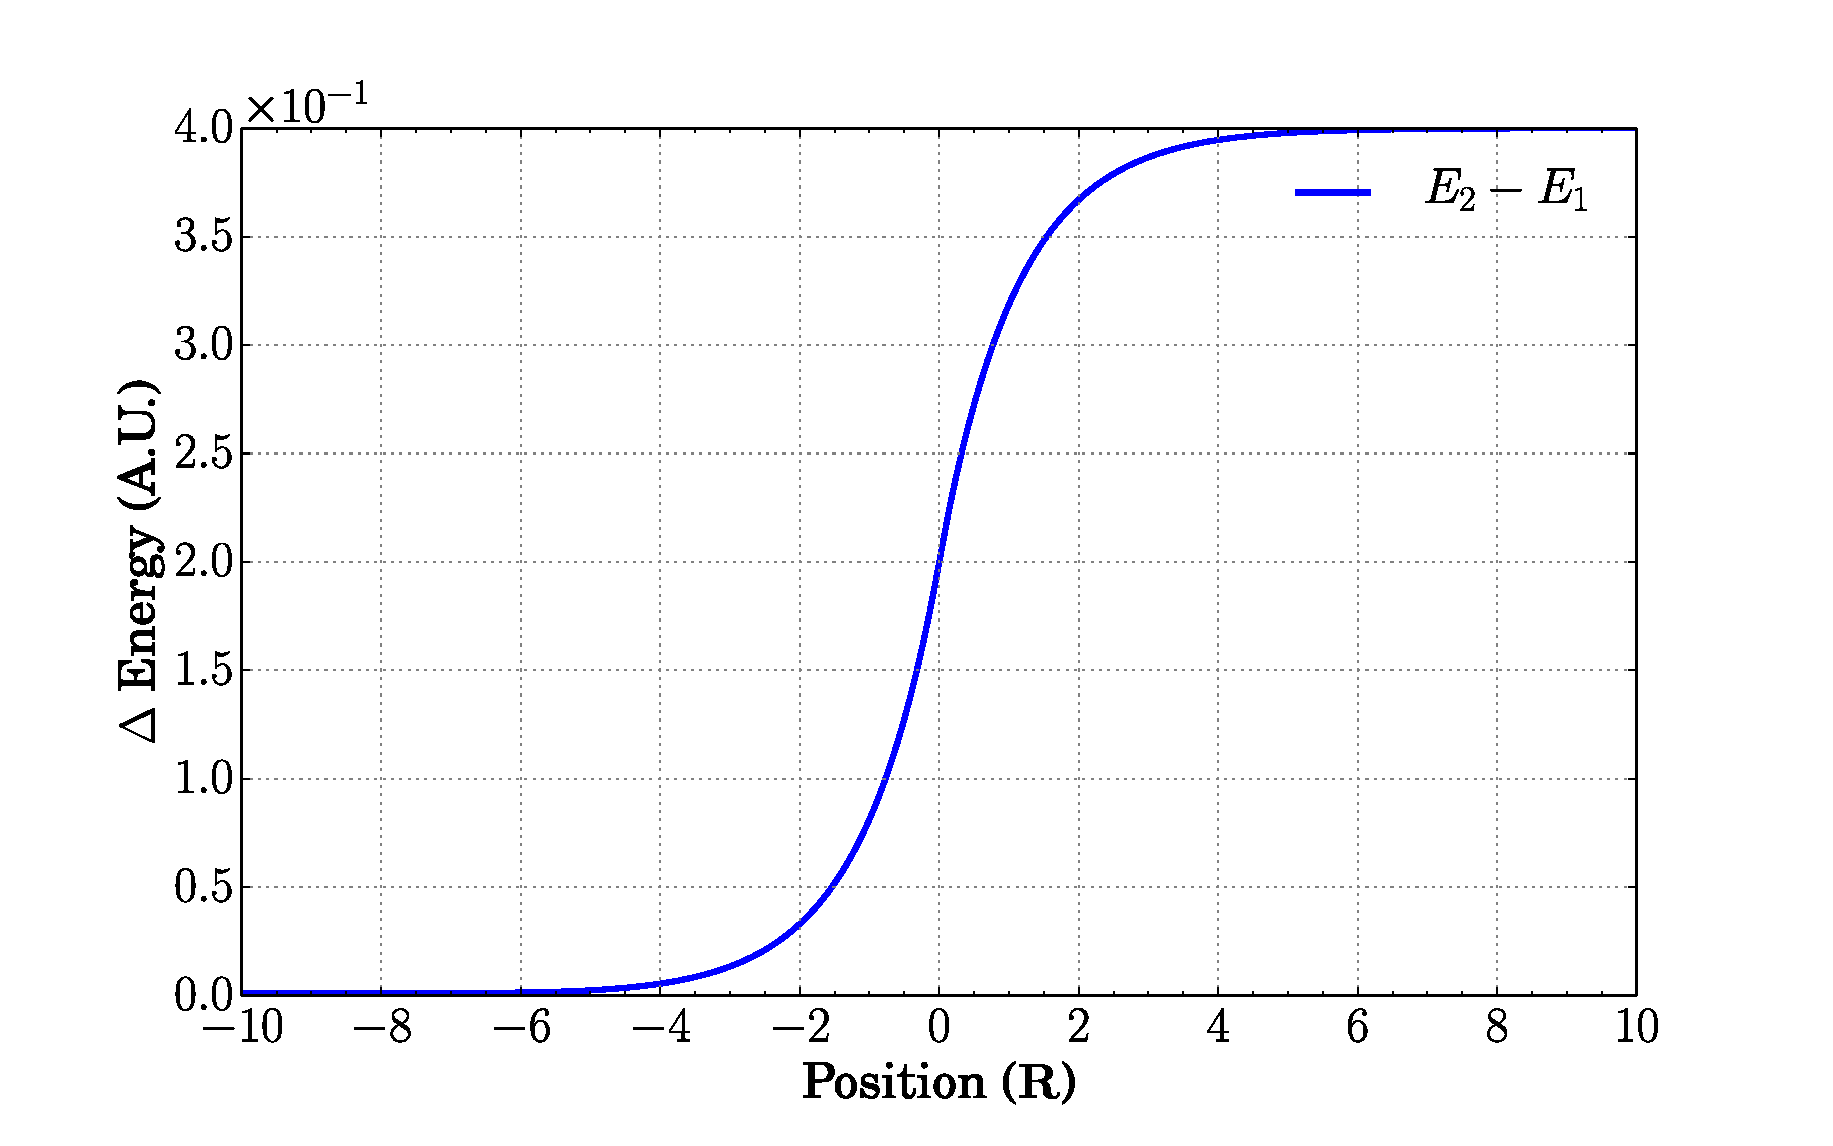
\includegraphics[scale=0.5]{del_aecpes.eps}
\caption[Extended coupling: energy difference between adiabatic PES]{Energy difference between adiabatic PES.}
\label{f:delapesec}
\end{figure}
%
\subsubsection{Equations of Motion}
%
The equations of motion are:
\begin{subequations}
\begin{align}
\dot{R} & = \frac{\chi}{\mu} \\
\dot{P} & = \frac{A B C}{2} \left(
\begin{cases}
e^{-C R} &\quad R\geq 0\\
e^{C R} &\quad R<0
\end{cases}
\right)
\left(\frac{(p_{1}^{2} + x_{1}^{2} - p_{2}^{2} - x_{2}^{2})\cdot \phi}{\eta} -\frac{(p_{2} x_{1} - p_{1} x_{2})\cdot \chi}{\mu \cdot \eta^{2}}
\right)\\
\dot{x_{1}} & = -\zeta\cdot x_{2} - \eta\cdot p_{1} \\
\dot{p_{1}} & = -\zeta\cdot p_{2} + \eta\cdot x_{1} \\
\dot{x_{2}} & = \zeta\cdot x_{1} + \eta\cdot p_{2} \\
\dot{p_{2}} & = \zeta\cdot p_{1} - \eta\cdot x_{2}~,
\end{align}
\end{subequations}
where,
\begin{subequations}
\begin{align}
&\phi = \frac{
B\begin{cases}
(2 - e^{-C R}) &\quad R \geq 0\\
e^{C R} &\quad R < 0
\end{cases}}{A} \\
&\eta = A\sqrt{1 + \phi^{2}}\\
&\chi = P + \frac{1}{2}(p_{2} x_{1} - p_{1} x_{2}) \arctan(\phi)\\
&\zeta =\frac{\arctan(\phi)\cdot \chi}{2 \mu}~.
\end{align}
\end{subequations}
%
\subsection{Spin-Boson Model for Condensed-Phase Dynamics}\label{sb:sb}
%
This problem is vastly different from the others. In our case, the model describes a 1D system of $ M $ coupled oscillators. More specifically, a one-dimensional lattice made up of $ M $ oscillating nuclei which posses bulk electronic states. What is measured here are not trajectories, but rather the time-dependent difference in the probability of finding the system in either of two electronic states; when the initial state $ =1 $, $ D(t) = P_{1\leftarrow 1} - P_{2\leftarrow 1}$, when the initial state $ =2 $, $ D(t) = P_{1\leftarrow 2} - P_{2\leftarrow 2}$.
%
\subsubsection{Potential Energy Surfaces}
%
The diabatic PES are defined as follows:
\begin{subequations}\label{eq:sbpes1}
\begin{align}
H_{11}(\bm{Q}) &= V_{0}(\bm{Q}) + V_{1}(\bm{Q}) + \epsilon \\
H_{22}(\bm{Q}) &= V_{0}(\bm{Q}) - V_{1}(\bm{Q}) - \epsilon \\
H_{12}(\bm{Q}) &= H_{12}(\bm{Q}) = \Delta~,
\end{align}
\end{subequations}
where,
\begin{subequations}\label{eq:sbpes2}
\begin{align}
V_{0}(\bm{Q}) &= \sum\limits_{k=1}^{M} \frac{1}{2} m_{k} \omega_{k}^{2} Q_{k}^{2} \\
V_{1}(\bm{Q}) &= \sum\limits_{k=1}^{M} c_{k} Q_{k}~.
\end{align}
\end{subequations}
For our purposes, the frequencies, $ \omega_{k} $, are uniformly distributed in the interval $ [0.01 \omega_{c},~4 \omega_{c}] $ \cite{spin-boson}, where $ \omega_{c} $ is known as the \emph{characteristic frequency}, and defines the system's overall time scale. The observant reader will realise this does not make a lot of sense on its own, because not all frequencies contribute to a system's energy in equal amounts. Which is why the coupling parameters, $ c_{k} $, are chosen so they obey the distribution:
\begin{align}\label{eq:sb_dd}
J(\omega) = \frac{\pi}{2} \sum\limits_{k=1}^{M} \frac{c_{k}^{2}}{m_{k} \omega_{k}}  \delta(\omega - \omega_{k})~,
\end{align}
where $ J(\omega) $ is an Ohmic distribution defined as:
\begin{align}\label{eq:sb_cd}
J(\omega) = \frac{\pi}{2} \alpha \omega \exp\left(-\frac{\omega}{\omega_{c}}\right)~,
\end{align}
where $ \alpha $ is the Kondo parameter (a coupling strength parameter). After equating \cref{eq:sb_dd,eq:sb_cd}, and integrating with respect to $ \omega $, we find the values of $ c_{k} $ to be:
\begin{subequations}
\begin{align}
c_{k} = \sqrt{\frac{2}{\pi} \Delta \omega m_{k} \omega_{k} J(\omega_{k})} 
&= \omega_{k} \sqrt{\alpha \Delta \omega m_{k} \exp\left(-\frac{\omega_{k}}{\omega_{c}}\right)} \\
\Delta \omega &= \frac{\omega_{max} - \omega_{min}}{M - 1}~.
\end{align}
\end{subequations}

The initial electronic conditions are initiated in the same manner as before. However, the nuclear ones are not. As stated before, the model describes oscillating nuclei in a 1D lattice, and their momenta and positions are assumed to follow the Wigner distribution:
\begin{subequations}
\begin{align}
\rho(\bm{P},\bm{Q}) &= \prod\limits_{k=1}^{M} \exp\left(-a_{k} \frac{P_{k}^{2}}{2 m_{k}}\right) \exp\left(-a_{k} \frac{1}{2} m_{k} \omega_{k}^{2} \left[Q_{k} + \frac{c_{k}}{m_{k} \omega_{k}^{2}}\right]^{2} \right)\\
a_{k} &= \frac{2}{\omega_{k}} \tanh\left(\frac{\beta \omega_{k}}{2}\right)~.
\end{align}
\end{subequations}
Which, in reality, is a bivariate normal distribution. Fortunately, the lack of a covariant term implies that positions and momenta can be independently sampled from normally distributed random numbers. In other words, the nuclei follow independent normal distributions for their momenta and positions. It is also worth noting that the argument for the total distribution is basically a scaled quasiclassical analogue of the quantum harmonic oscillator Hamiltonian operator ($ \hat{H} = \frac{\hat{p}^{2}}{2m} + \frac{1}{2} m \omega^{2} \hat{x}^{2}$), which makes a lot of intuitive sense, because it means the nuclear parameters are sampled according to the oscillators' normally distributed kinetic energy.

Sampling is done in the traditional way: assuming $ X $ is a normally distributed random number with unitary standard deviation and mean equal to zero, a normally distributed random number $ G $ with standard deviation equal to $ \sigma $ and mean equal to $ \mu $ can be calculated by $ G = \sigma X + \mu $. Given the definition of the normal distribution,
\begin{align}
G(x, \mu, \sigma) = \frac{1}{\sigma \sqrt{2\pi}} \exp\left[- \frac{(x-\mu)^{2}}{2 \sigma^{2}}\right]~,
\end{align}
the standard deviations and mean values of the nuclei's momenta and positions are:
\begin{subequations}
\begin{align}
&\sigma_{P_{k}} = \sqrt{\frac{m_{k} \omega_{k}}{2 \tanh\left(\frac{\beta \omega_{k}}{2}\right)}}\\
&\mu_{P_{k}} = 0\\
&\sigma_{Q_{k}} = \sqrt{\frac{1}{2 m_{k} \omega_{k} \tanh\left(\frac{\beta \omega_{k}}{2}\right)}}\\
&\mu_{Q_{k}} = -\frac{c_{k}}{m_{k} \omega_{k}^{2}}~.
\end{align}
\end{subequations}

The Gaussian sampling algorithm used, is a modified version of the Ziggurat algorithm originally written by George Marsaglia and Wai Wan Tsang\footnote{See \url{http://people.sc.fsu.edu/~jburkardt/f\_src/ziggurat/ziggurat.html}.}. The modification randomises the seed every time the subroutine is initialised, thus providing the accurate pseudo-random numbers necessary for reliable Monte Carlo simulations.
%
\subsubsection{Equations of Motion}
%
The equations of motion are obtained in exactly the same way as before (using the diabatic Hamiltonian), only we have defined $ M = 100 $ so there are 100 nuclear degrees of freedom (DOFs), which means there are 100 equations of motion for position and another 100 for momentum, giving a grand total of 204 equations. The nuclear equations of motion---as well as $ H_{11} $ and $ H_{22} $---are implemented as {\color{DarkViolet}\texttt{do}} loops:
\begin{subequations}
\begin{align}
\dot{Q_{j}} &= \frac{P_{j}}{m_{j}}\\
\dot{P_{j}} &= -m_{j}\omega_{j}^{2}Q_{j} - \frac{1}{2}c_{j}\cdot(p_{1}^{2} + x_{1}^{2} - p_{1}^{2} - x_{2}^{2})\\
\dot{x_{1}} & = p_{1}(V_{1} + \epsilon) + p_{2}\Delta\\
\dot{p_{1}} & = -x_{1}(V_{1} + \epsilon) - x_{2}\Delta\\
\dot{x_{2}} & = -p_{2}(V_{1} + \epsilon) + p_{1}\Delta\\
\dot{p_{2}} & = x_{2}(V_{1} + \epsilon) - x_{1}\Delta~.
\end{align}
\end{subequations}
%
\section{Code Structure}
%
\begin{itemize}
\item Main program.
\begin{enumerate}
\item Call data collection subroutine.
\item Call print PES and DPES subroutine.
\end{enumerate}
\item Data collection subroutine.
\begin{enumerate}
\item Declare and initialise variables.
\item Open output file.
\item Write heading on file.
\item Define value of initial momentum.
\item Call Monte-Carlo averaging routine.
\item Write final results.
\begin{itemize}
\item Repeat 4. to 6. for other initial momentum values.
\end{itemize}
\end{enumerate}
\end{itemize}

\begin{itemize}
\item Monte-Carlo averaging subroutine.
\begin{enumerate}
\item Declare and intialise variables.
\item Define Monte-Carlo steps loop.
\begin{enumerate}
\item Call solution subroutine.
\item Add results.
\end{enumerate}
\item Average results with the number of Monte-Carlo steps.
\item Calculate transition probabilities for reflection and transmission.
\end{enumerate}
\end{itemize}

\begin{itemize}
\item Solution subroutine.
\begin{enumerate}
\item Declare and initialise variables.
\item Define and calculate initial conditions and window functions.
\item Define integration loop.
\begin{enumerate}
\item Call RK4G subroutine using the appropriate equations of motion as argument.
\item Check for reflection, exit loop if the particle was reflected.
\item Update the initial conditions for next integration step.
\end{enumerate}
\item Calculate final values for the acceptance criteria.
\item Calculate final window functions.
\item Calculate results for the Monte-Carlo averaging subroutine.
\end{enumerate}
\end{itemize}

\begin{itemize}
\item Equations of motion subroutine.
\begin{enumerate}
\item Define and initialise variables.
\item Define equations of motion.
\end{enumerate}
\end{itemize}

\begin{itemize}
\item Runge-Kutta 4 Gill numerical integration routine (RK4G).
\begin{enumerate}
\item Define and initialise variables.
\item Call equations of motion subroutine.
\begin{itemize}
\item Calculate the intermediate step for all independent variables.
\end{itemize}
\item Repeat 2. for every intermediate step.
\item Calculate the final value of every independent variable, to be used in the next integration step.
\end{enumerate}
\end{itemize}

\begin{itemize}
\item PES and DPES printing subroutine.
\begin{enumerate}
\item Define and initialise variables.
\item Define loop to print all functions.
\begin{enumerate}
\item Open relevant output file.
\item Call PES and DPES subroutines.
\item Write numerical values of each PES and DPES function, evaluated at any given distance.
\begin{itemize}
\item Repeat b) and c) for all desired distances.
\end{itemize}
\end{enumerate}
\end{enumerate}
\end{itemize}

\begin{itemize}
\item PES or DPES subroutines.
\begin{enumerate}
\item Define and initialise variables.
\item Check which PES or DPES are required.
\item Define PES or DPES.
\end{enumerate}
\end{itemize}
%
%-------------Results--------------%
\chapter{Results}\label{c:r}
%
The code was found to scale linearly with integration step, number of Monte-Carlo repetitions (MC reps) and number of cores used---which are the best case scenarios; this is what everyone who does programming hopes for. There were some minor variations from exact linearity but their randomness is due to the model's Monte-Carlo characteristics. It was also found that accuracy is more dependent on the number of MC reps than the size of the integration step, $ h $. In fact, the integration step could be made relatively large (how large depends on the problem) without significantly affecting accuracy, but drastically reducing execution time. There was also no significant difference between using $ \gamma = \dfrac{\sqrt{3}-1}{2} $ and $ \gamma = 0.366 $ \cite{project}---the actual value is very similar, but there is no need to evaluate square roots and divisions all the time if we use the numerical approximation; \cite{project} gives the theoretical justification for this value, but it can be adjusted on a case by case basis. Accuracy was also not noticeably affected by parallel runs, presumably due to the random number generator used---which is thread safe---but not optimal for parallelisation, because it generates numbers in sequence from a single source rather than in parallel\footnote{See \url{https://gcc.gnu.org/onlinedocs/gfortran/RANDOM_005fNUMBER.html}} (this only affects execution speed).

The number of MC reps $ = 15000 $ and the value of $ \gamma = 0.366 $ unless stated otherwise. Reflections are denoted as $ R $ and transmissions as $ T $, electronic transitions from an initial state, $ i $, to a final state, $ f $, are denoted as $ f \leftarrow i $. 

All calculations were carried out on a computer equipped with an Intel i7-3770k processor overclocked to 4.3 GHz, $ 2\times4 $ Gb Kingston RAM overclocked to 1660 MHz, mounted on a Gigabyte GA-Z77X-UD3H motherboard (the video card is irrelevant because all calculations were processor bound), all functioning on the {\ubuntumono ubuntu 14.04 LTS} operating system. The code was compiled with the \texttt{gfortran} module from the \texttt{GNU} compiler collection \texttt{gcc 4.9.2} \footnote{See \url{https://gcc.gnu.org/}}.
%
\section{Single Avoided Crossing}
%
Being the simplest system, the single avoided crossing problem was used to test code's robustness. \Crefrange{f:scc}{f:sc1t} show results for $ i = 1 $ while \crefrange{f:sci2}{f:sc2t} show the results for $ i = 2 $. Despite this being the simplest problem tackled herein, it presents some fairly interesting behaviours. The results for when $ i = 1 $ are very similar---though not exactly the same---as those found in \cite{project}. However, this is most likely down to the fact that they used $ 50000\text{--}100000$ trajectories as well as there being a strong possibility that the compiler, RNG, and integration step differ.

\Cref{f:scc} shows a comparison between two different integration step sizes, there is no significant difference in accuracy between them both.
\begin{figure}
\centering
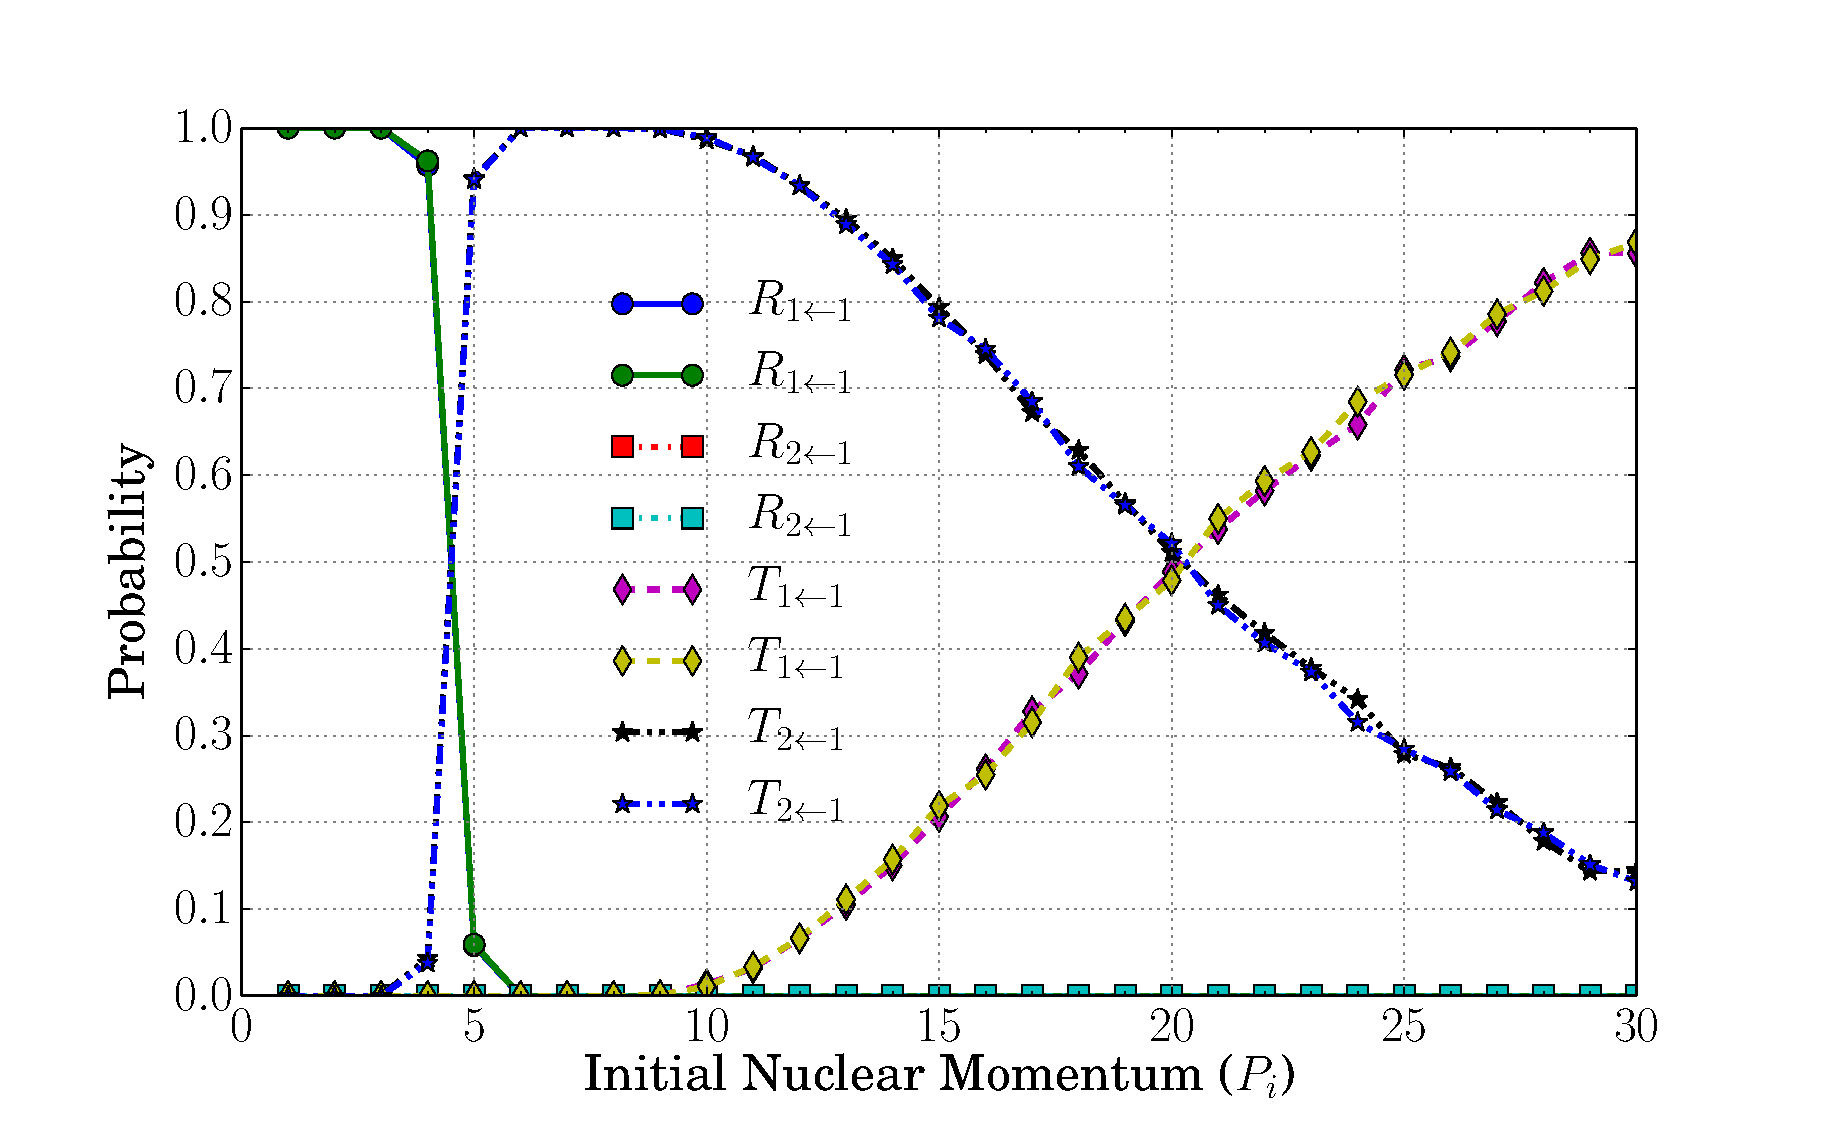
\includegraphics[scale=0.5]{sc_prob_1oip_vs_1o5ip.eps}
\caption[Single avoided crossing: comparison between integration step size. $ i = 1 $.]{Comparison between $ h = (5P_{i})^{-1} $ (appearing first in the legend) and $ h = P_{i}^{-1} $. $ \gamma = \frac{\sqrt{3} - 1}{2}$ in both cases. $ i = 1 $.}
\label{f:scc}
\end{figure}
\Cref{f:sclh} shows the results for very large values of $ h $, there is no significant difference between using large or small values of $ h $.
\begin{figure}
\centering
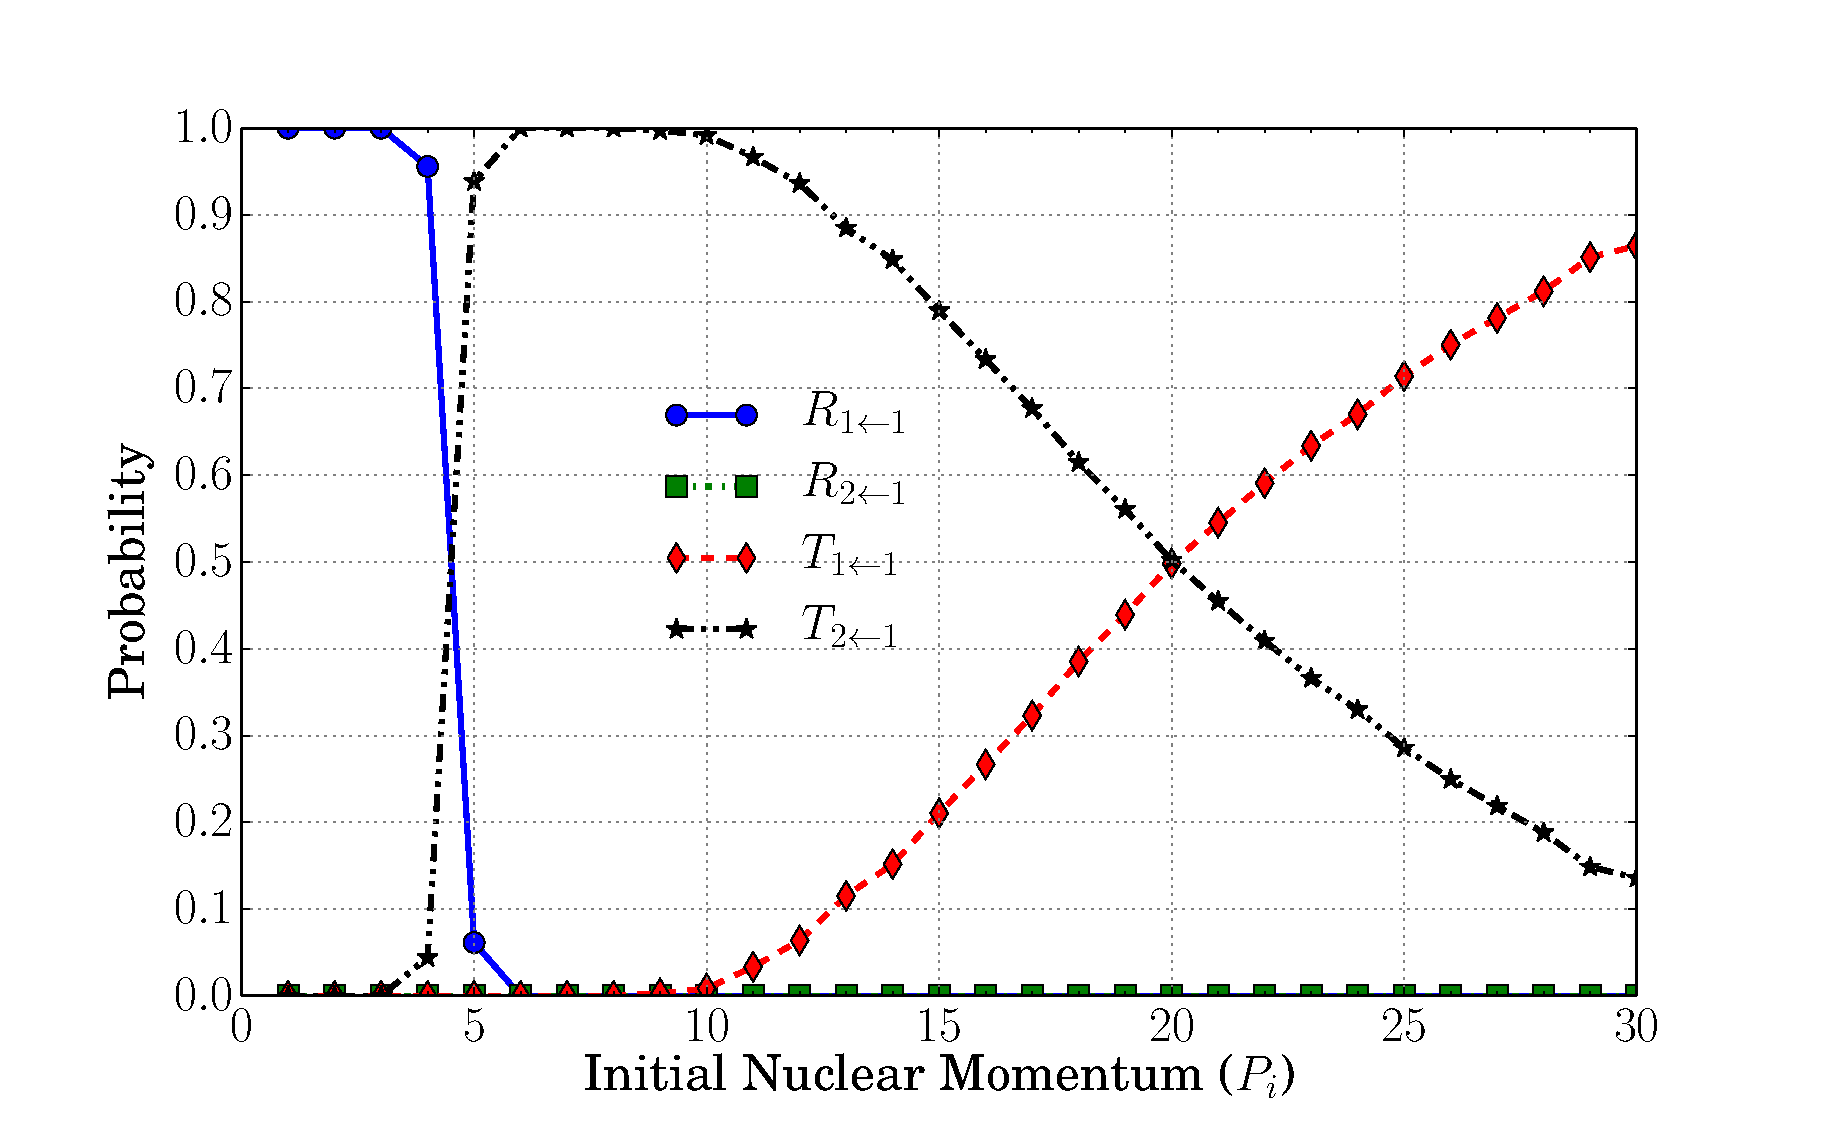
\includegraphics[scale=0.5]{sc_prob_lh.eps}
\caption[Single avoided crossing: large integration step. $ i = 1 $.]{Transition probabilities for $ R $ and $ T $, $ h = (0.012P_{i})^{-1} $. $ i = 1 $. Computational time $ = 8$ min. $ 7.35 $ s.}
\label{f:sclh}
\end{figure}
\Cref{f:scpar} shows a two-core parallel run, there is no significant difference in accuracy compared to single-core calculations.
\begin{figure}
\centering
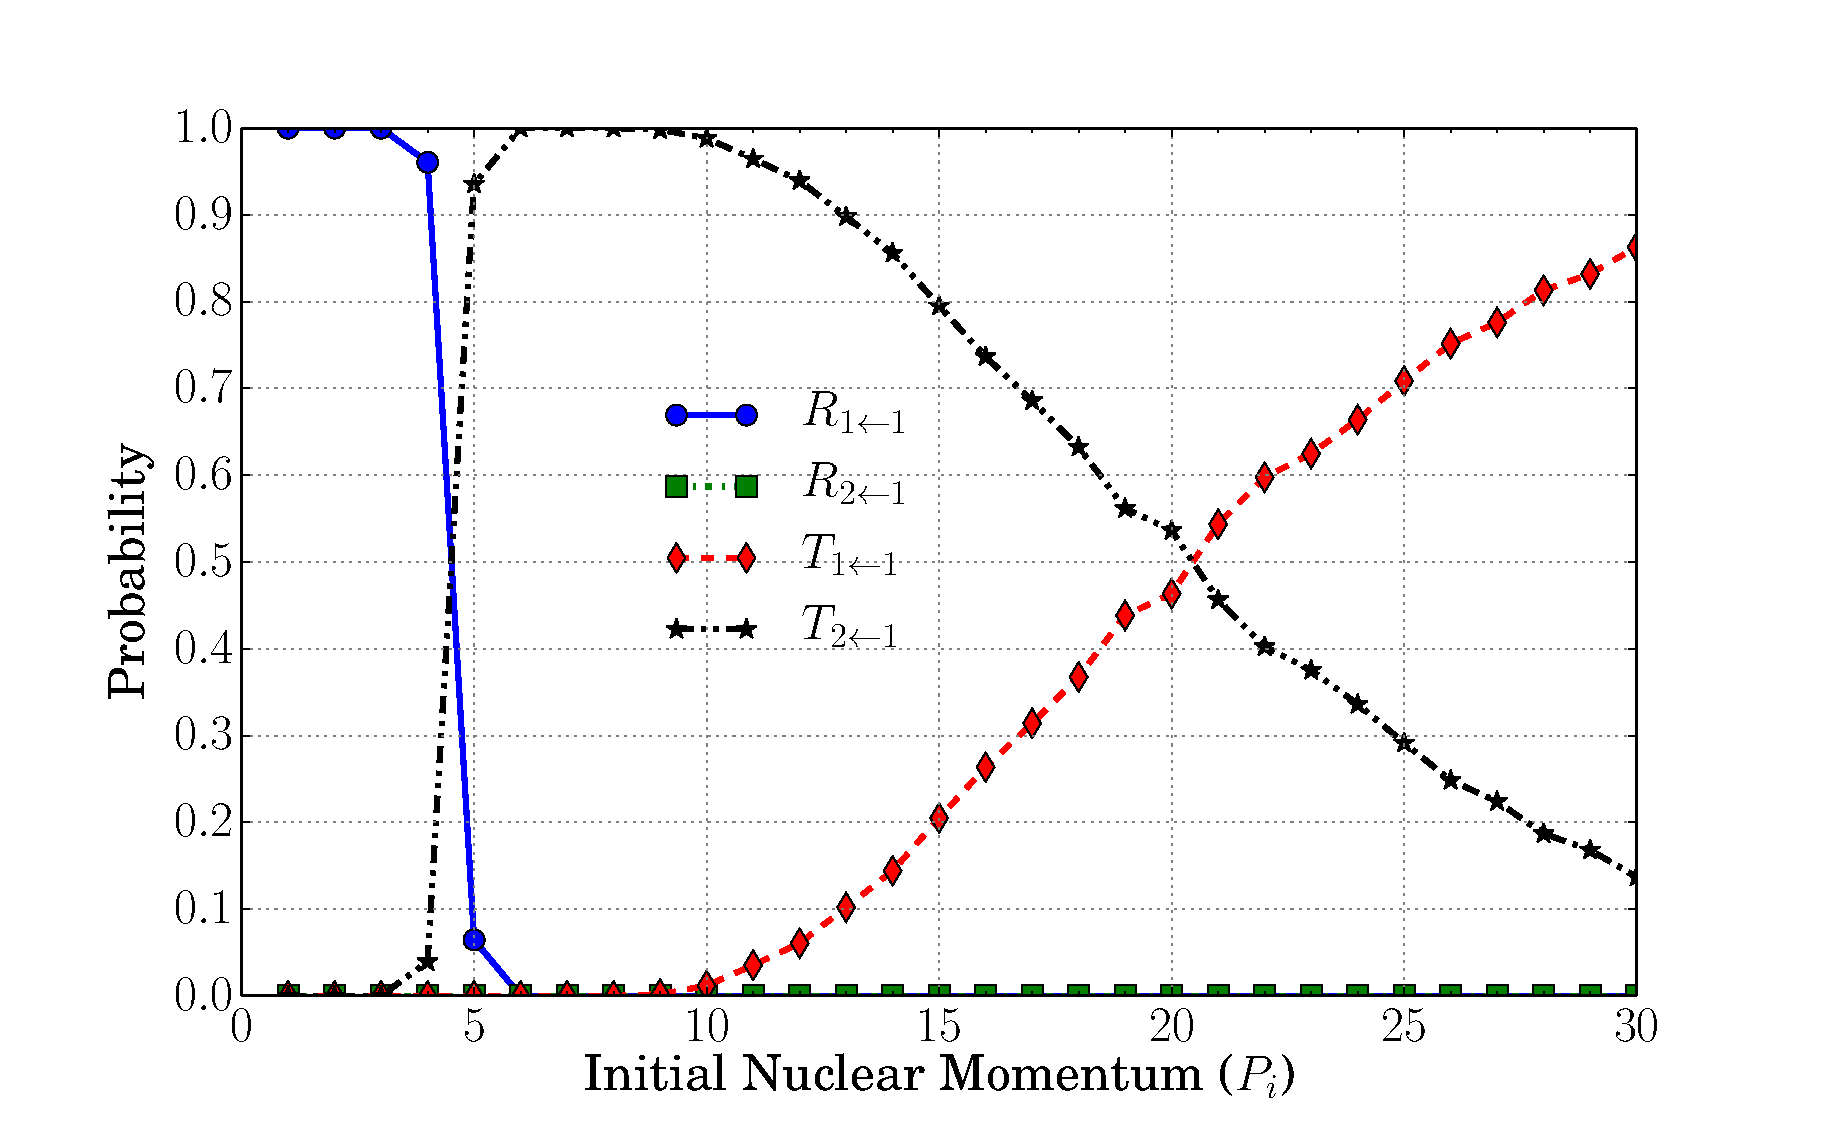
\includegraphics[scale=0.5]{sc_prob_parallel.eps}
\caption[Single avoided crossing: parallel calculations. $ i = 1 $.]{Parallel calculations on two cores (7500 MC reps per core), $ h = (5P_{i})^{-1} $. No significant deviation from single-core calculations. $ i = 1 $.}
\label{f:scpar}
\end{figure}

First, we shall tackle the case where $ i = 1 $. The behaviour of \roo, whose probability is seen to rapidly decline as nuclear momentum increases, can be explained by referring back to \cref{f:pessc}. For small values of nuclear momentum, there is not enough kinetic energy to scale over the potential barrier (akin to an `activation energy') and continue in the original direction, thus the particle is reflected back, preventing its electronic states from interacting, as seen in \cref{sf:scr11,sf:scr11e}. \rto~is similarly explained; once there is enough kinetic energy to reach a point where a transition is likely to happen, there would also be enough energy to continue on to the other side. Thus \rto~remains relatively close to zero throughout. The others can be explained by the fact that transition probabilities are not only a function of the distance between adiabatic PES, but also of the time it takes the particle to move away from regions where electronic coupling is strong. This explains the behaviour of \tto~and \too. For \tto~lower nuclear momenta allow more time for an electronic transition to occur as seen in \cref{sf:sct21,sf:sct21e}; however, after a certain value of nuclear momentum, it begins to decrease in favour of \too~because the particle travels so fast, it cannot interact long enough to undergo an electronic transition, as shown in \cref{sf:sct11,sf:sct21e}.

\begin{figure}
\begin{subfigure}[t]{0.5\textwidth}
\centering
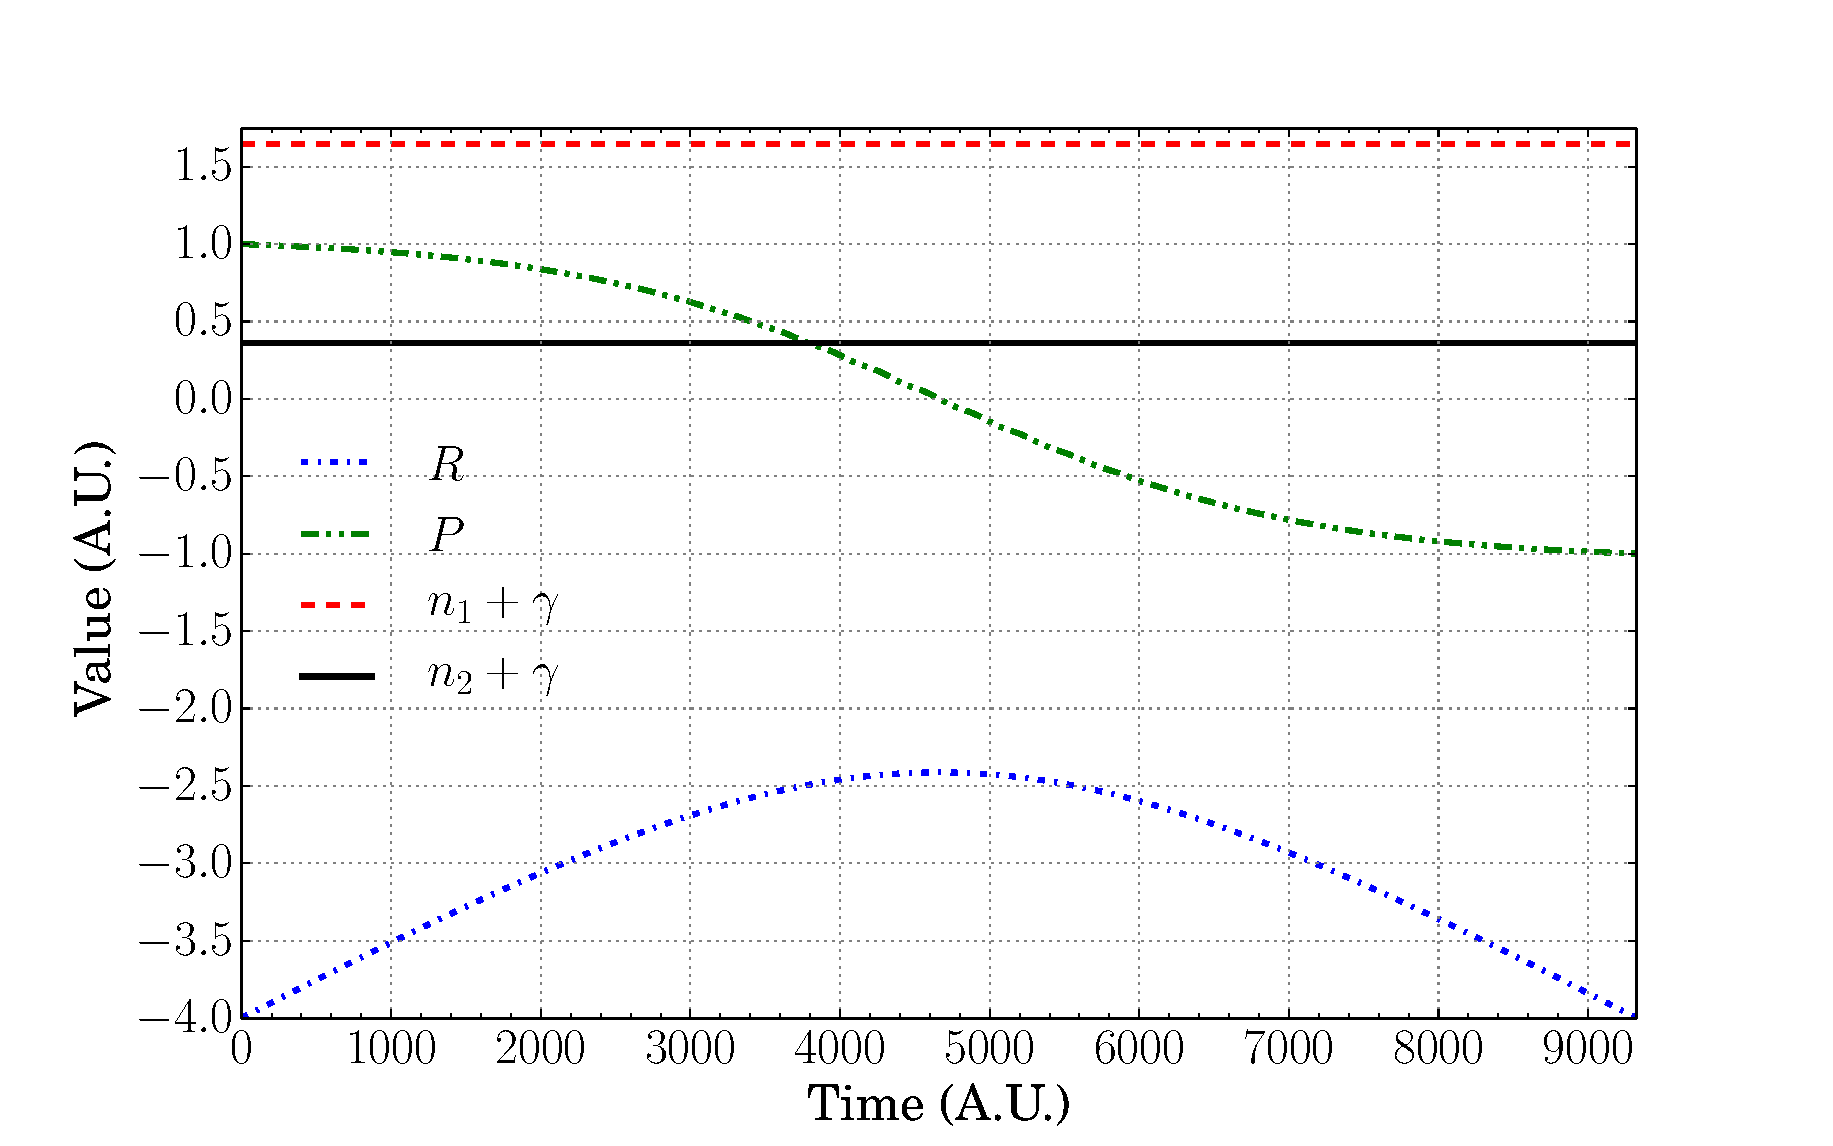
\includegraphics[width=\textwidth]{sc_traj_r11.eps}
\caption[Single avoided crossing: \roo~trajectory.]{\roo~trajectory.}
\label{sf:scr11}
\end{subfigure}
~
\begin{subfigure}[t]{0.5\textwidth}
\centering
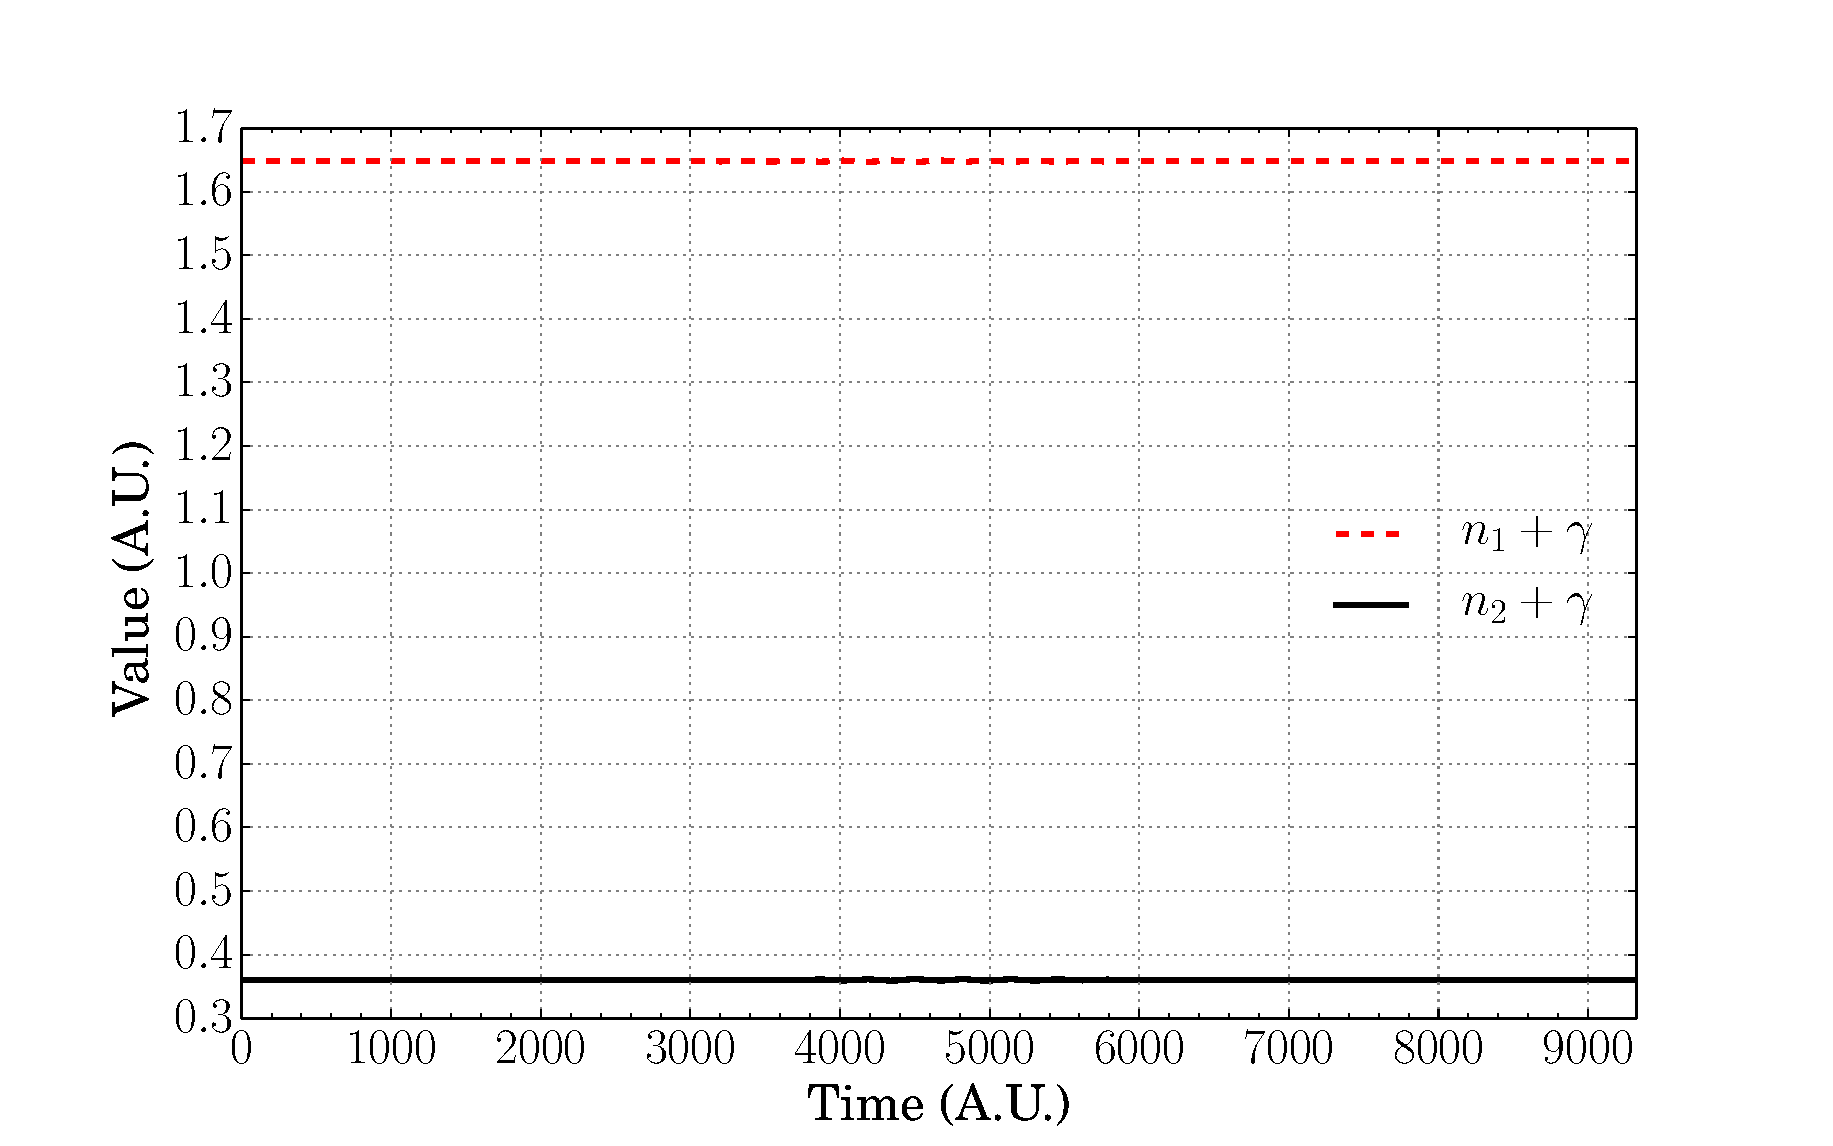
\includegraphics[width=\textwidth]{sc_traj_r11_e.eps}
\caption[Single avoided crossing: \roo~trajectory, zoom into $ n_{1}~\text{and}~n_{2} $.]{\roo~trajectory, zoom into $ n_{1}~\text{and}~n_{2} $.}
\label{sf:scr11e}
\end{subfigure}

\begin{subfigure}[t]{0.5\textwidth}
\centering
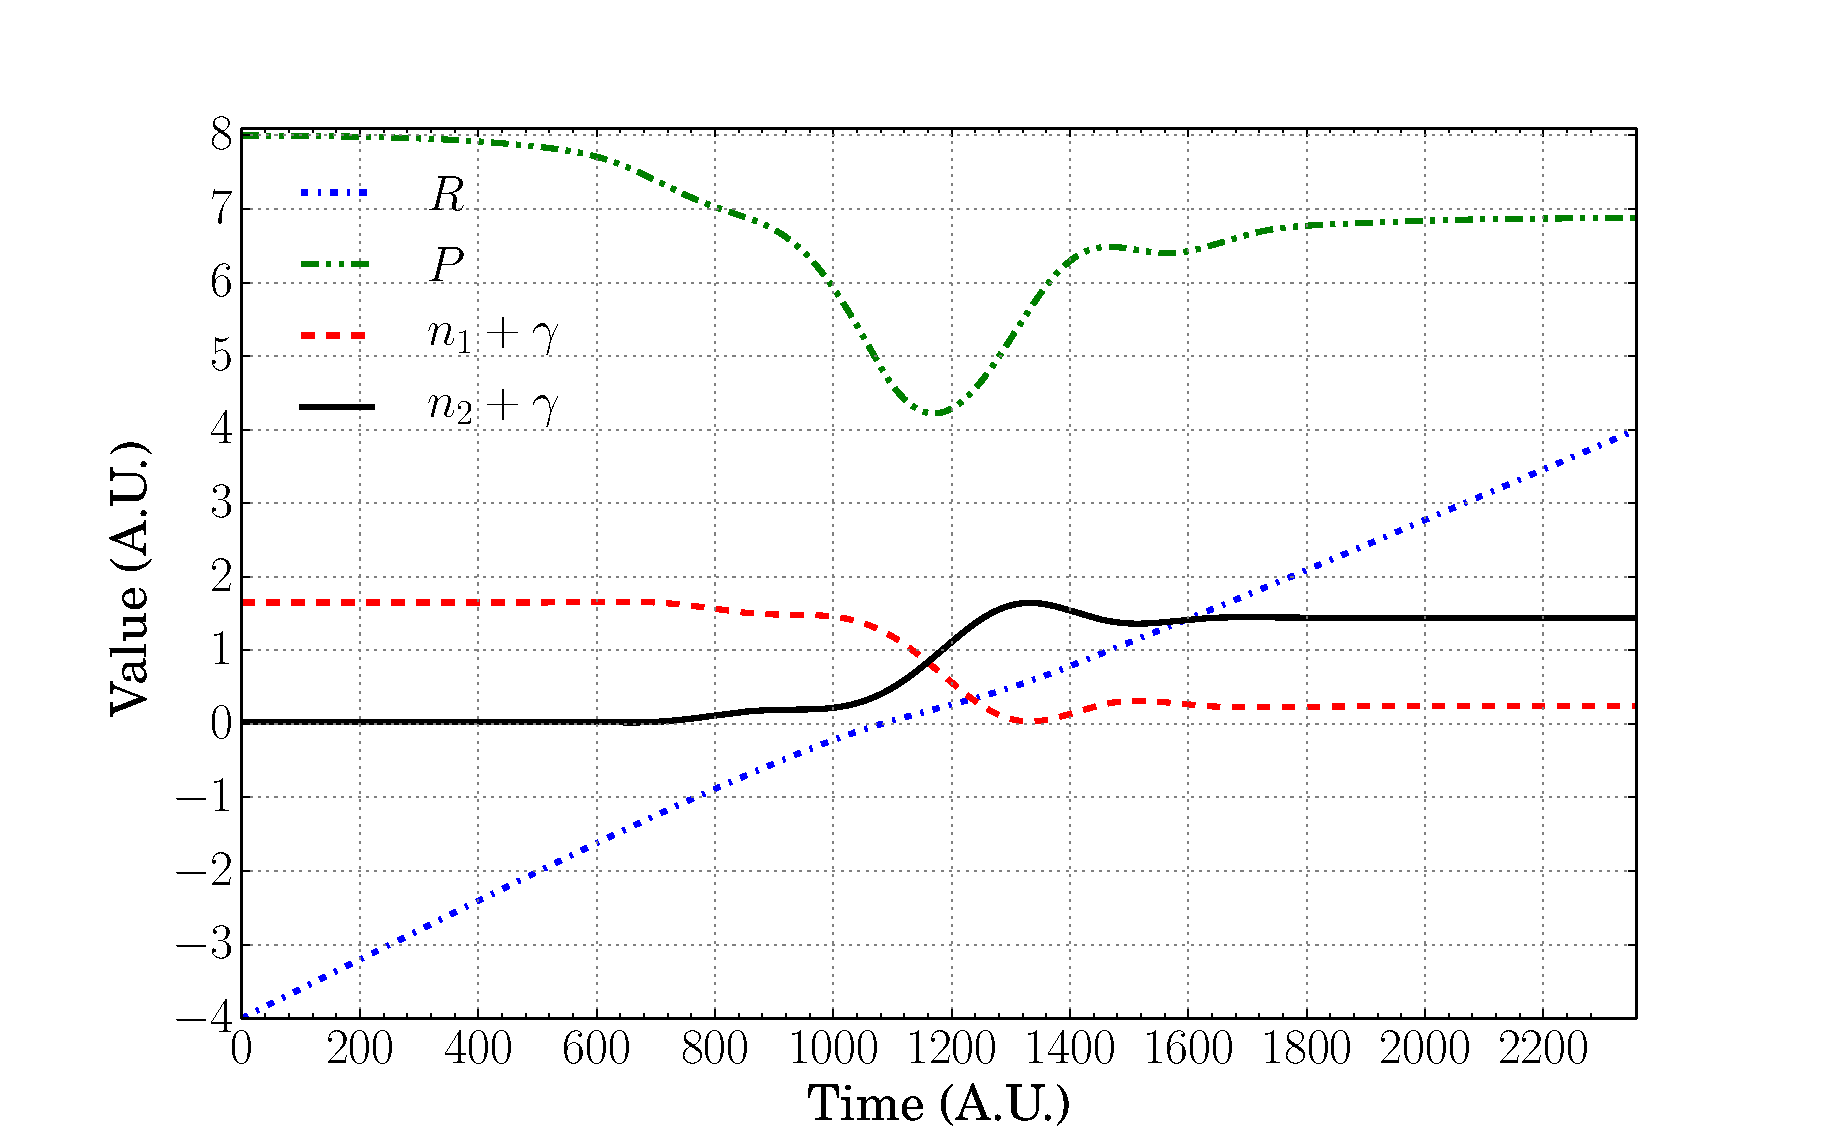
\includegraphics[width=\textwidth]{sc_traj_t21.eps}
\caption[Single avoided crossing: \tto~trajectory.]{\tto~trajectory.}
\label{sf:sct21}
\end{subfigure}
~
\begin{subfigure}[t]{0.5\textwidth}
\centering
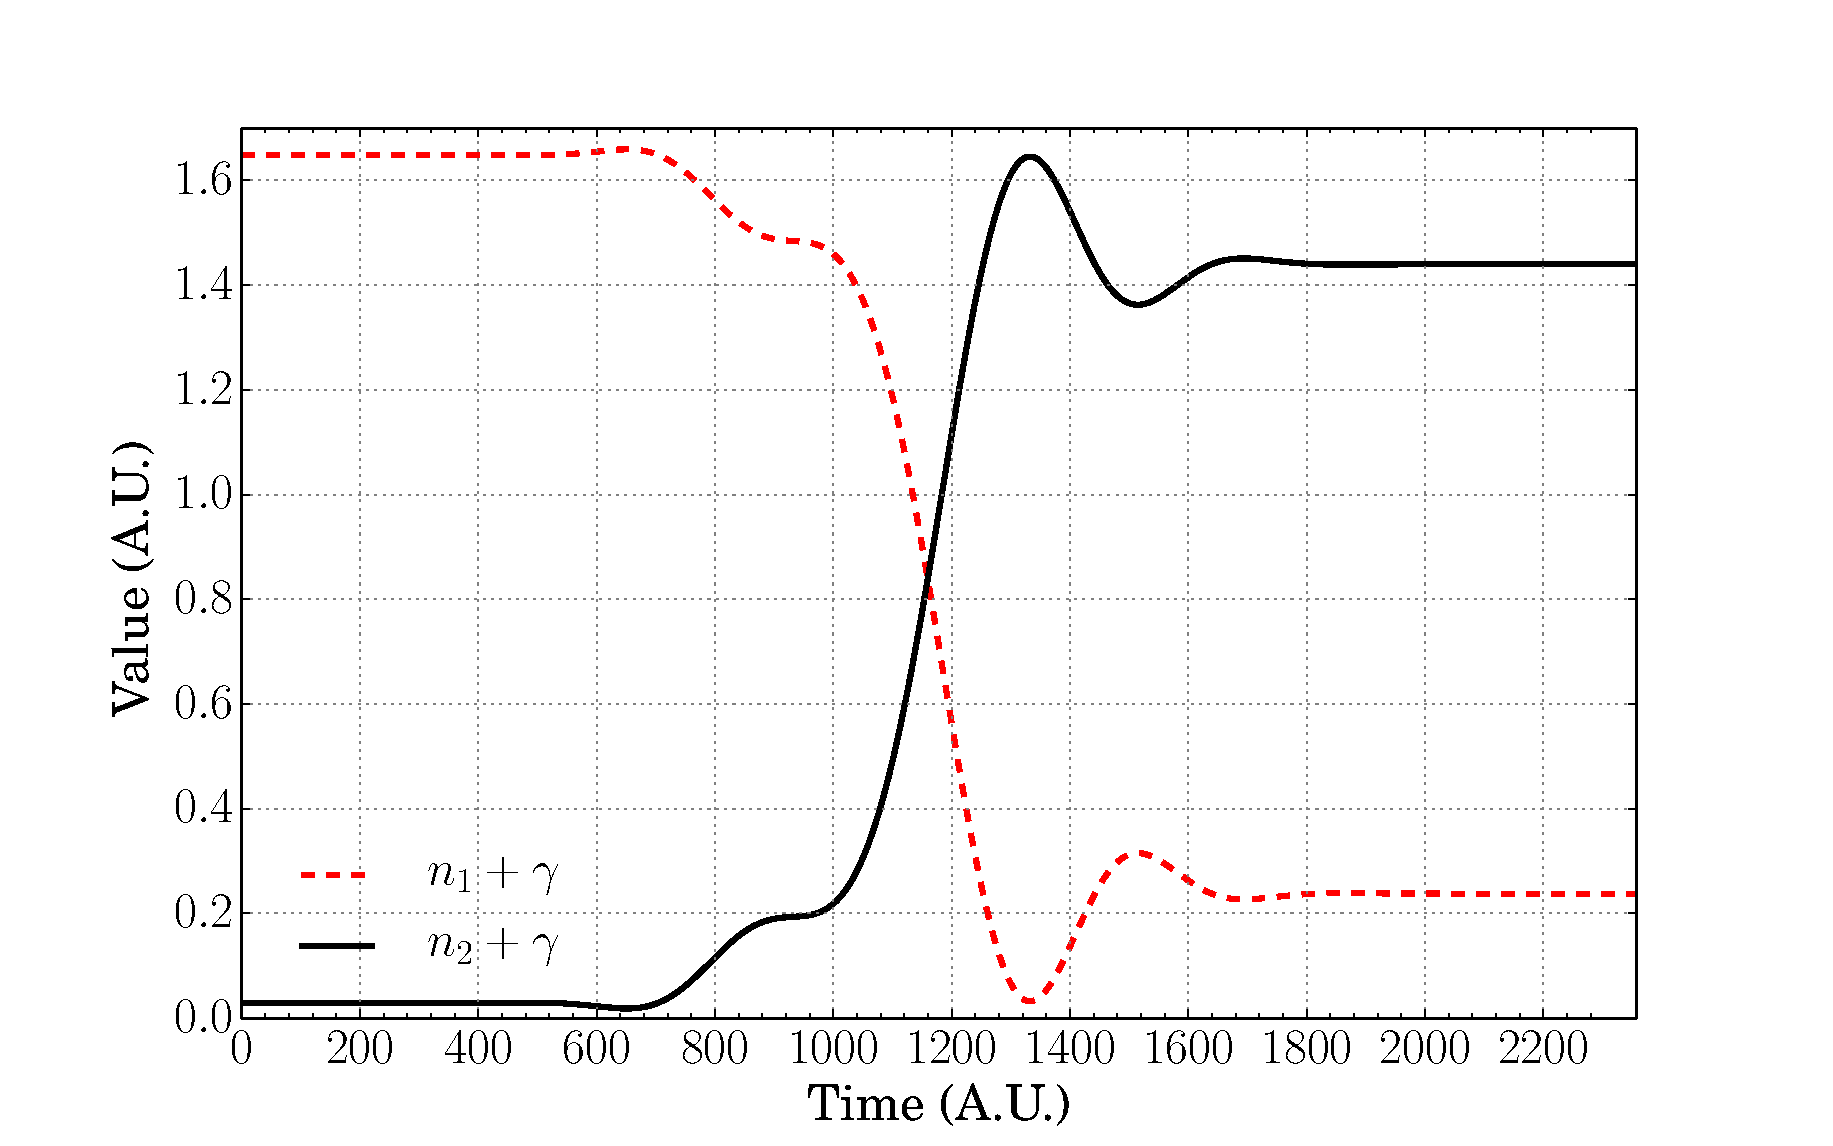
\includegraphics[width=\textwidth]{sc_traj_t21_e.eps}
\caption[Single avoided crossing: \tto~trajectory, zoom into $ n_{1}~\text{and}~n_{2} $.]{\tto~trajectory, zoom into $ n_{1}~\text{and}~n_{2} $.}
\label{sf:sct21e}
\end{subfigure}

\begin{subfigure}[t]{0.5\textwidth}
\centering
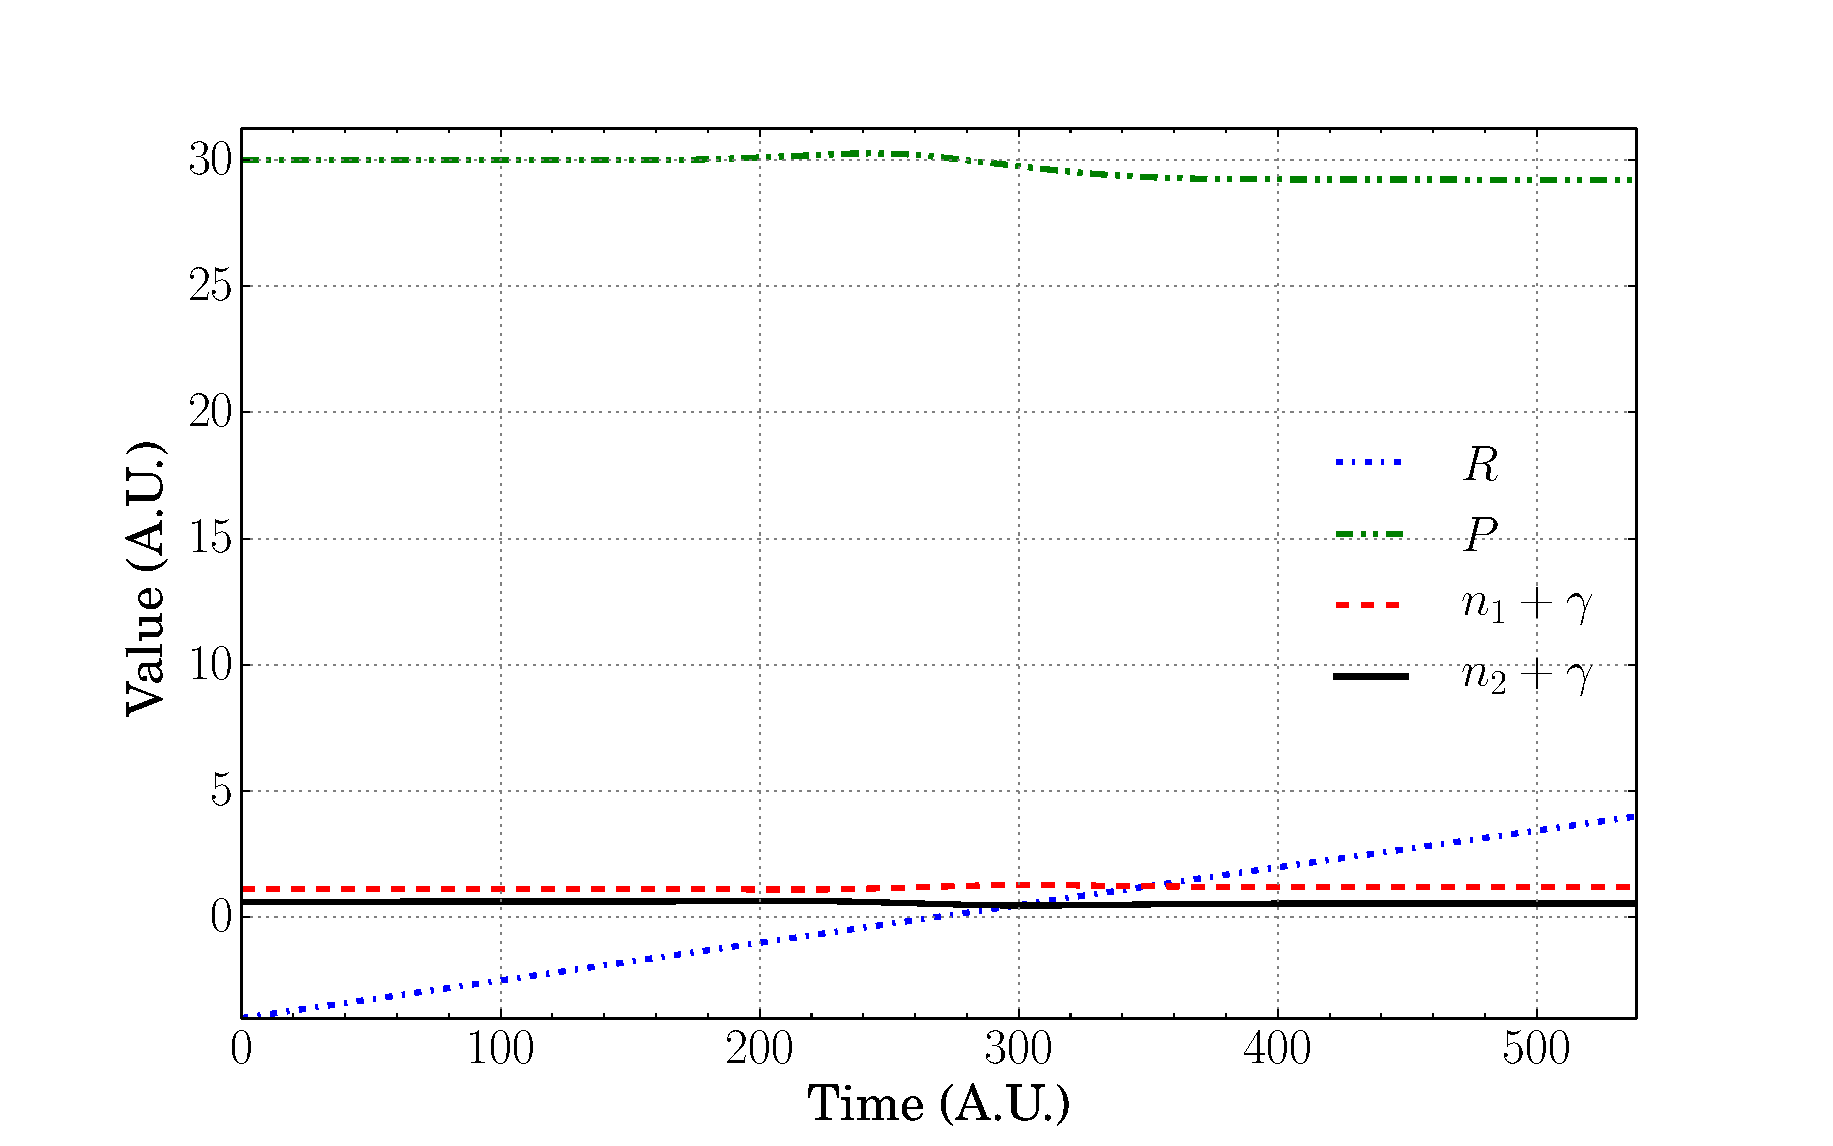
\includegraphics[width=\textwidth]{sc_traj_t11.eps}
\caption[Single avoided crossing: \too~trajectory.]{\too~trajectory.}
\label{sf:sct11}
\end{subfigure}
~
\begin{subfigure}[t]{0.5\textwidth}
\centering
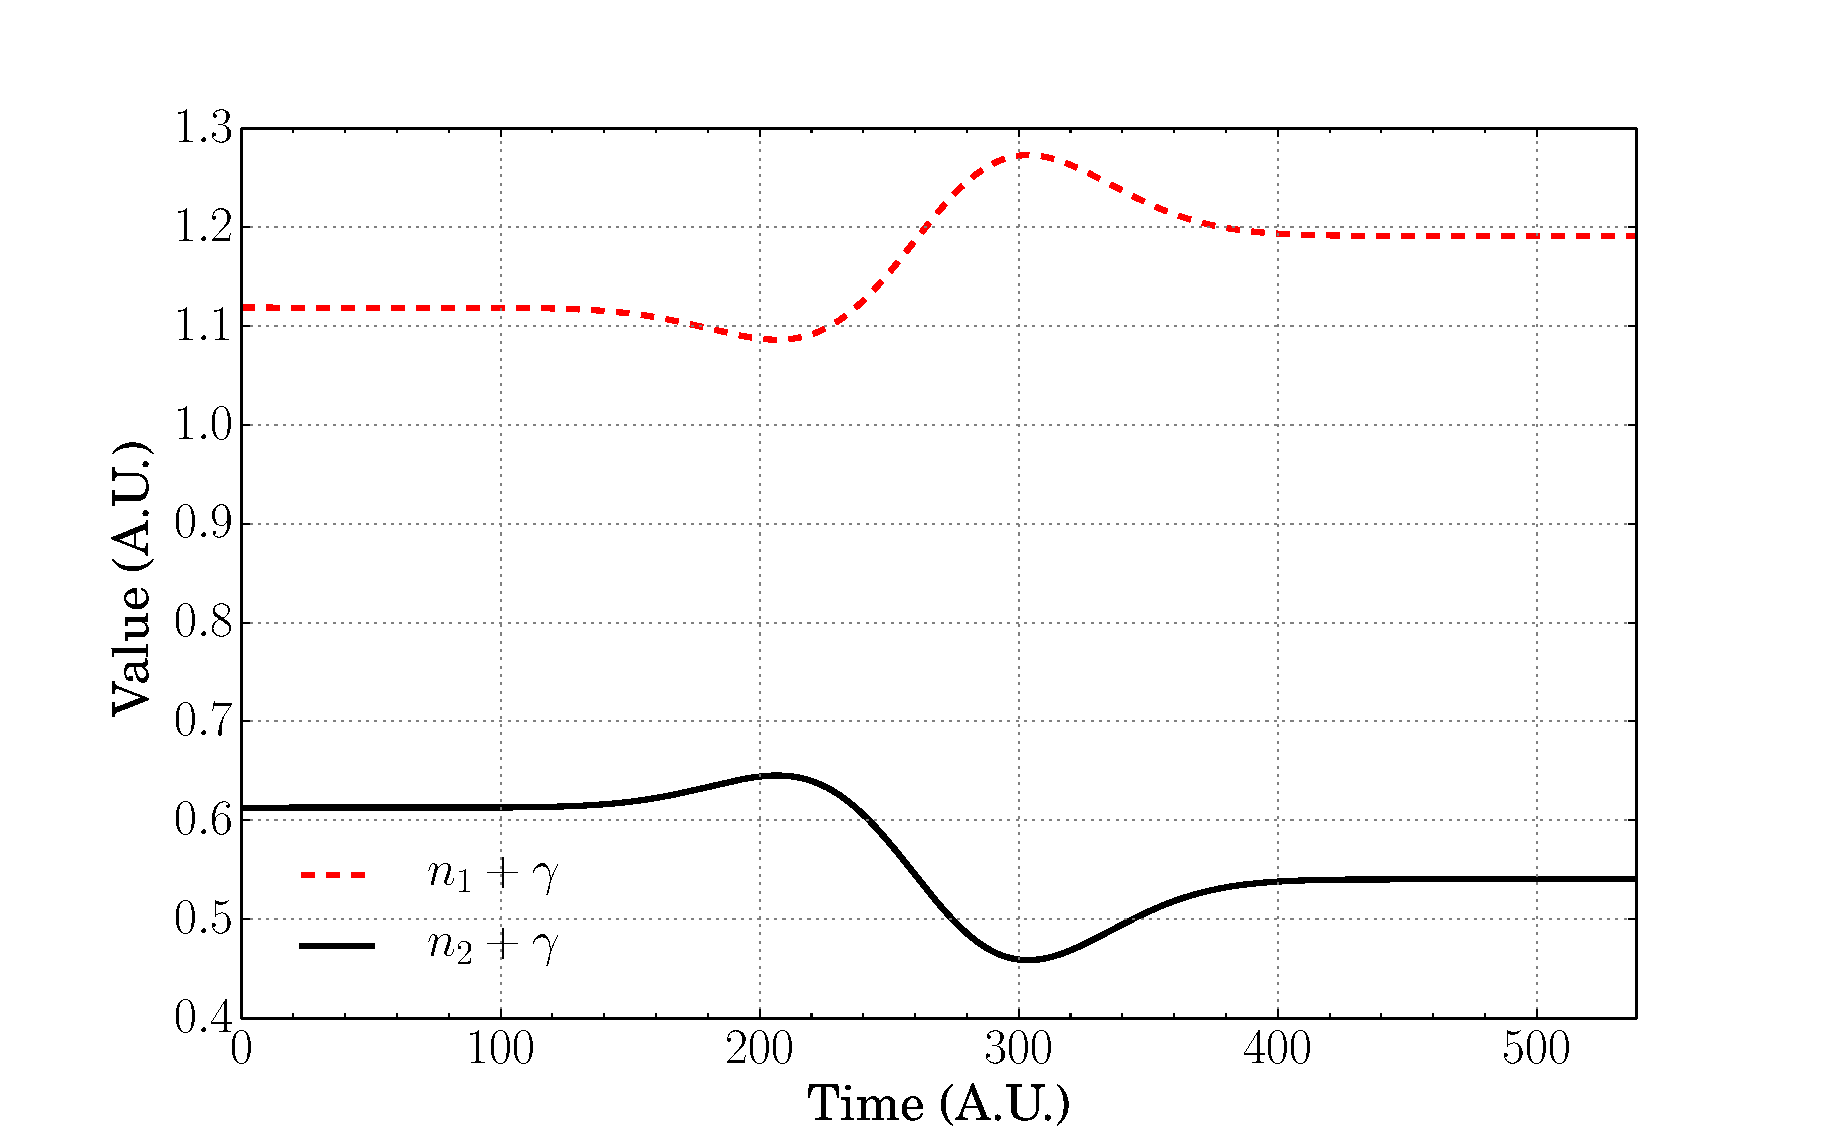
\includegraphics[width=\textwidth]{sc_traj_t11_e.eps}
\caption[Single avoided crossing: \too~trajectory, zoom into $ n_{1}~\text{and}~n_{2} $.]{\too~trajectory, zoom into $ n_{1}~\text{and}~n_{2} $.}
\label{sf:sct11e}
\end{subfigure}
\caption[Single avoided crossing: trajectory examples. $ i = 1 $.]{Trajectory examples.  $ i = 1 $.}
\label{f:sc1t}
\end{figure}

\begin{figure}
\centering
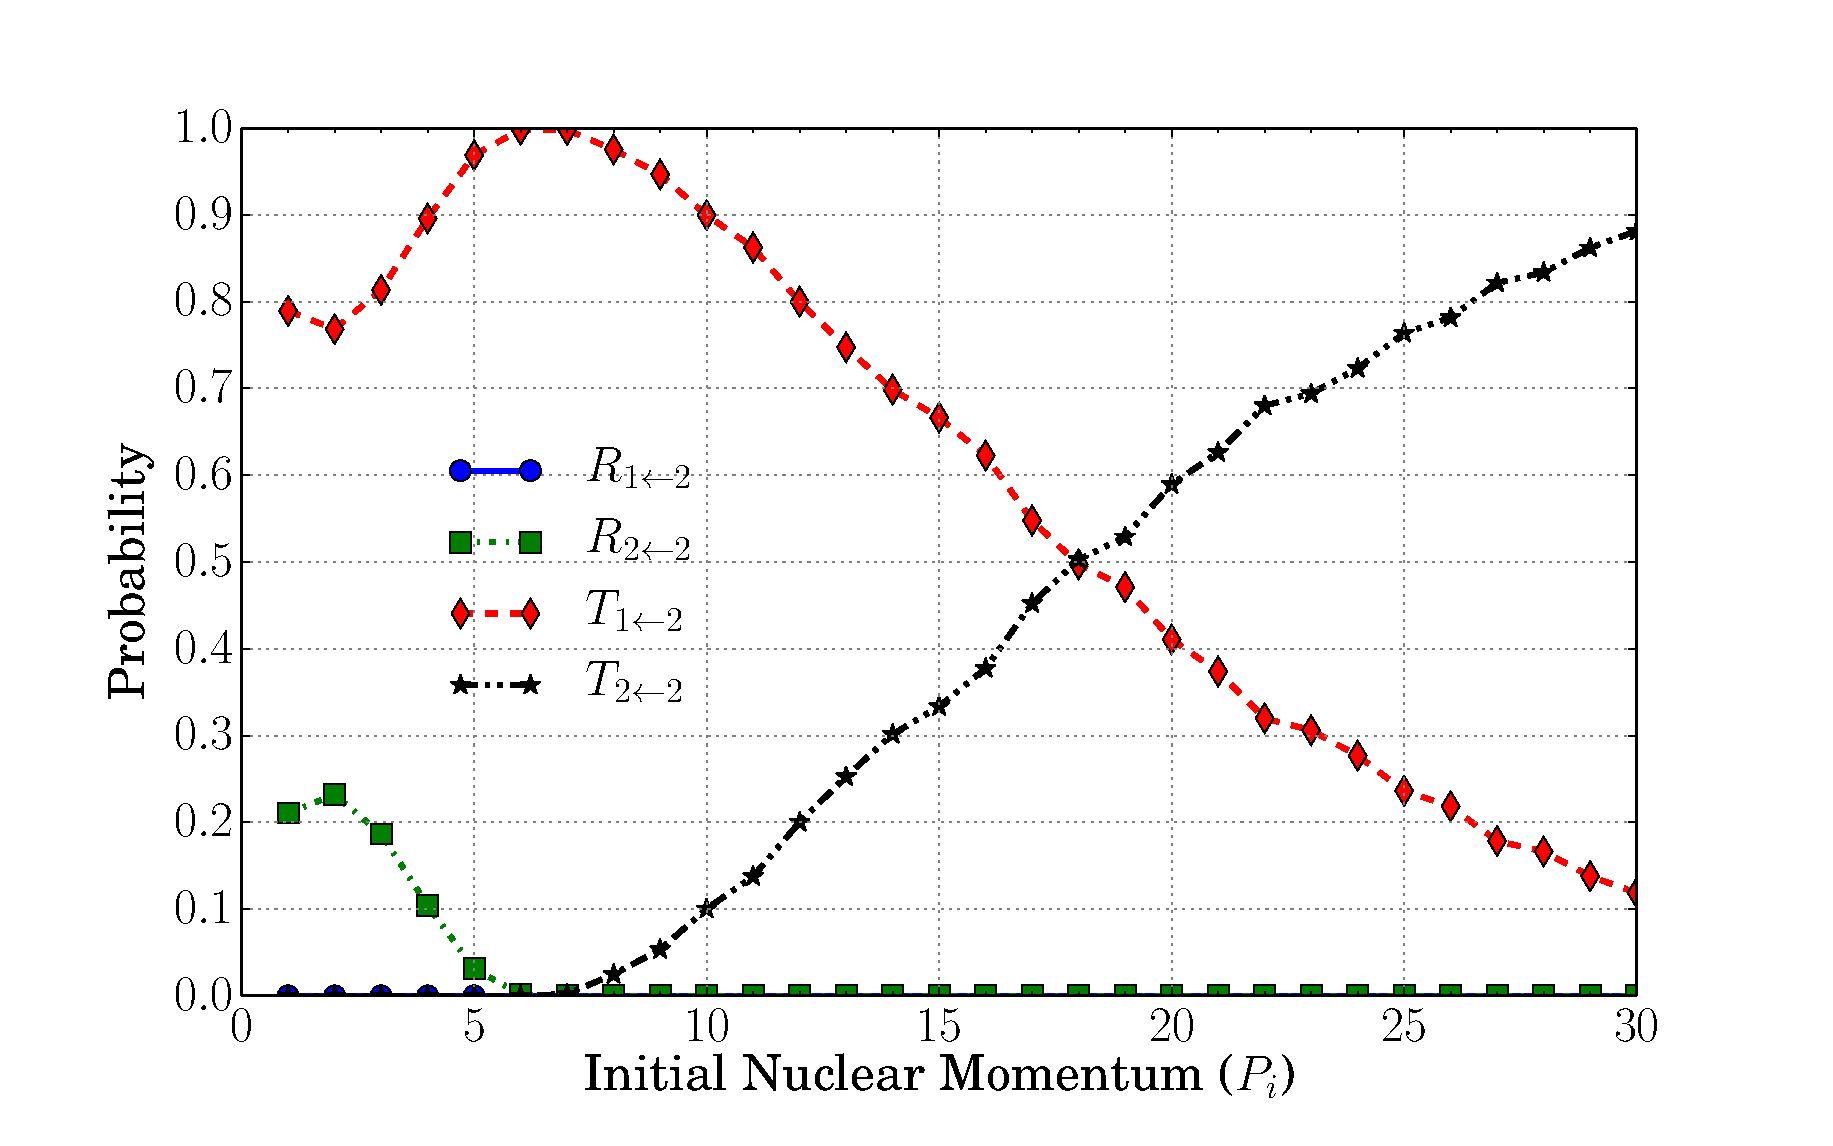
\includegraphics[scale=0.5]{sc_prob_i2.eps}
\caption[Single avoided crossing. $ i = 2 $]{Transition probabilities for $ R $ and $ T $, $ h = (0.012P_{i})^{-1} $. $ i = 2 $. Computational time $ = 7$ min. $ 47.74 $ s.}
\label{f:sci2}
\end{figure}
In the case of $ i = 2 $ only one graph is provided (\cref{f:sci2}), as tests yielded similar results as previously demonstrated. In this case, the system's behaviour is more nuanced, but is explained by the same reasons. The \rot~transition remains effectively zero throughout, because at such low nuclear momenta two things can happen: the particle can be reflected back along $ H_{22} $ by the off-diagonal PES---corresponding to the \rtt~transition, as seen in \cref{sf:scr22,sf:scr22e} (in fact the particle keeps getting bounced back time and time again until it finally leaves the integration area as a reflection)---or it moves down to the lower energy state, where the surplus potential energy is converted into kinetic energy (conservation of energy) and a \tot~transition is observed, as seen in \cref{sf:sct12,sf:sct12e}. For higher values of nuclear momentum, the particle has enough energy to be transmitted, but there is not enough time for the particle's electronic states to interact, and a \ttt~is observed instead, shown in \cref{sf:sct22,sf:sct22e}. The higher the nuclear momentum the less time there is and the likelier this transition becomes.

\begin{figure}
\begin{subfigure}[t]{0.5\textwidth}
\centering
\includegraphics[width=\textwidth]{sc_traj_r22.eps}
\caption[Single avoided crossing: \rtt~trajectory.]{\rtt~trajectory.}
\label{sf:scr22}
\end{subfigure}
~
\begin{subfigure}[t]{0.5\textwidth}
\centering
\includegraphics[width=\textwidth]{sc_traj_r22_e.eps}
\caption[Single avoided crossing: \rtt~trajectory, zoom into $ n_{1}~\text{and}~n_{2} $.]{\rtt~trajectory, zoom into $ n_{1}~\text{and}~n_{2} $.}
\label{sf:scr22e}
\end{subfigure}

\begin{subfigure}[t]{0.5\textwidth}
\centering
\includegraphics[width=\textwidth]{sc_traj_t12.eps}
\caption[Single avoided crossing: \tot~trajectory.]{\tot~trajectory.}
\label{sf:sct12}
\end{subfigure}
~
\begin{subfigure}[t]{0.5\textwidth}
\centering
\includegraphics[width=\textwidth]{sc_traj_t12_e.eps}
\caption[Single avoided crossing: \tot~trajectory, zoom into $ n_{1}~\text{and}~n_{2} $.]{\tot~trajectory, zoom into $ n_{1}~\text{and}~n_{2} $.}
\label{sf:sct12e}
\end{subfigure}

\begin{subfigure}[t]{0.5\textwidth}
\centering
\includegraphics[width=\textwidth]{sc_traj_t22.eps}
\caption[Single avoided crossing: \ttt~trajectory.]{\ttt~trajectory.}
\label{sf:sct22}
\end{subfigure}
~
\begin{subfigure}[t]{0.5\textwidth}
\centering
\includegraphics[width=\textwidth]{sc_traj_t22_e.eps}
\caption[Single avoided crossing: \ttt~trajectory, zoom into $ n_{1}~\text{and}~n_{2} $.]{\ttt~trajectory, zoom into $ n_{1}~\text{and}~n_{2} $.}
\label{sf:sct22e}
\end{subfigure}
\caption[Single avoided crossing: trajectory examples. $ i = 2 $.]{Trajectory examples. $ i = 2 $.}
\label{f:sc2t}
\end{figure}
%
\section{Double Avoided Crossing}\label{s:rdac}
%
\Crefrange{f:dc1}{f:dc1t} show results for $ i = 1 $ while \crefrange{f:dc2}{f:dc2t} show the results for $ i = 2 $. Again the results for when $ i = 1 $ are very similar---but not exactly the same---as those found in \cite{project}. Which can be attributed to the same factors as before. In our case $ E_{i} $ is the mean total initial energy, which could also contribute to the differences with published results.

\Cref{f:dc1} shows the results for small values of $ h $, while \cref{f:dclh} uses large values of $ h $. There is no significant difference between the two.
\begin{figure}
\centering
\includegraphics[scale=0.5]{dc_prob_1o5ip.eps}
\caption[Double avoided crossing: small integration step. $ i = 1 $.]{Transition probabilities for $ R $ and $ T $, $ h =(5 P_{i})^{-1} $. $ i = 1 $.}
\label{f:dc1}
\end{figure}
\begin{figure}
\centering
\includegraphics[scale=0.5]{dc_prob_lh.eps}
\caption[Double avoided crossing: large integration step. $ i = 1 $.]{Transition probabilities for $ R $ and $ T $ for $ h = (0.0125P_{i})^{-1} $. $ i = 1 $. Computational time $ = 7$ min. $ 33.29 $ s.}
\label{f:dclh}
\end{figure}
\Cref{f:dcpar} shows a two-core parallel run. There is no significant difference between this and \cref{f:dc1}.
\begin{figure}
\centering
\includegraphics[scale=0.5]{dc_prob_parallel.eps}
\caption[Double avoided crossing: parallel calculations. $ i = 1 $.]{Parallel calculations on two cores (7500 MC reps per core), $ h = (5P_{i})^{-1} $. No significant deviation from single-core calculations. $ i = 1 $.}
\label{f:dcpar}
\end{figure}

Once more, we shall first analyse the behaviour for $ i = 1 $, shown in \crefrange{f:dc1}{f:dcpar}. The lack of \roo~and \rto~transitions is easily explained by the fact there is no energy barrier in either the diagonal diabatic or adiabatic PES as seen in \cref{f:pesdc,f:apesdc}. Therefore the particle only requires a small amount of momentum for the it to be transmitted. In fact, in low momentum tests (\cref{sf:lm,sf:lme}), the particle was accelerated by the adiabatic energy wells (potential energy was transferred into kinetic energy). The other interesting feature is the presence the Stückelberg oscillations for both \too~and \tto, which are often attributed to quantum interference effects clearly seen in \cref{sf:t11e,sf:t21e}. In order to comprehend these one must only turn to \cref{f:delapesdc}, which shows the difference between adiabatic PES. One can see that $ E_{2} - E_{1} $ varies quickly and by relatively large amounts. For small momenta, the particle generally does not have enough energy to switch electronic states, leading to the relatively flat appearance of both \too~and \tto~from $ -4~\text{to}~-2 $. However, as momentum increases, there is enough energy to make one jump but not a lot to make the second one, leading to the behaviour seen from $ -2~\text{to}~-1 $. As momentum keeps increasing, there is enough energy for the second jump, and we get the behaviour we see from $ -1~\text{to}~0 $. Finally, when momentum is very large, the particle carries out one jump and does not linger long enough around the second minimum energy difference range, leading to the behaviour we see from $ 0~\text{to}~1 $. \Cref{f:dc1t} contains trajectory examples which support these allegations.

\begin{figure}
\begin{subfigure}[t]{0.5\textwidth}
\centering
\includegraphics[width=\textwidth]{dc_traj_t11.eps}
\caption[Double avoided crossing: \too~trajectory.]{\too~trajectory.}
\label{sf:t11}
\end{subfigure}
~
\begin{subfigure}[t]{0.5\textwidth}
\centering
\includegraphics[width=\textwidth]{dc_traj_t11_e.eps}
\caption[Double avoided crossing: \too~trajectory, zoom into $ n_{1}~\text{and}~n_{2} $.]{\too~trajectory, zoom into $ n_{1}~\text{and}~n_{2} $.}
\label{sf:t11e}
\end{subfigure}

\begin{subfigure}[t]{0.5\textwidth}
\centering
\includegraphics[width=\textwidth]{dc_traj_t21.eps}
\caption[Double avoided crossing: \tto~trajectory.]{\tto~trajectory.}
\label{sf:t21}
\end{subfigure}
~
\begin{subfigure}[t]{0.5\textwidth}
\centering
\includegraphics[width=\textwidth]{dc_traj_t21_e.eps}
\caption[Double avoided crossing: \tto~trajectory, zoom into $ n_{1}~\text{and}~n_{2} $.]{\tto~trajectory, zoom into $ n_{1}~\text{and}~n_{2} $.}
\label{sf:t21e}
\end{subfigure}

\begin{subfigure}[t]{0.5\textwidth}
\centering
\includegraphics[width=\textwidth]{dc_traj_low_momentum.eps}
\caption[Double avoided crossing: low nuclear momentum trajectory.]{Low nuclear momentum trajectory.}
\label{sf:lm}
\end{subfigure}
~
\begin{subfigure}[t]{0.5\textwidth}
\centering
\includegraphics[width=\textwidth]{dc_traj_low_momentum_e.eps}
\caption[Double avoided crossing: low nuclear momentum trajectory, zoom into $ n_{1}~\text{and}~n_{2} $.]{Low nuclear momentum trajectory, zoom into $ n_{1}~\text{and}~n_{2} $.}
\label{sf:lme}
\end{subfigure}
\caption[Double avoided crossing: trajectory examples. $ i = 1 $.]{Trajectory examples. $ i = 1 $.}
\label{f:dc1t}
\end{figure}

\begin{figure}
\centering
\includegraphics[scale=0.5]{dc_prob_i2.eps}
\caption[Double avoided crossing. $ i = 2 $]{Transition probabilities for $ R $ and$ T $ for $ h = (0.0125P_{i})^{-1} $. $ i = 2 $. Computational time $ = 10$ min. $ 41.63 $ s.}
\label{f:dc2}
\end{figure}
When the $ i = 2 $ as is the case in \cref{f:dc2}, the behaviour is very similar but inverted with respect to $ i = 1 $. In other words, the transmission which preserves the initial state, \ttt~in \cref{f:dc2}, is very similar in shape to the transmission which preserves the initial state, \too~in \cref{f:dc1}. And the transmission which does not preserve the initial state, \tot~in \cref{f:dc2}, is also very qualitatively similar to the transition which does not preserve the initial state, \tto~in \cref{f:dc1}. Which means they have similar explanations; the only variation being the precise points at which these `domains' appear. Trajectory examples are provided in \cref{f:dc2t}.

\begin{figure}
\begin{subfigure}[t]{0.5\textwidth}
\centering
\includegraphics[width=\textwidth]{dc_traj_t12.eps}
\caption[Double avoided crossing: \tot~trajectory.]{\tot~trajectory.}
\end{subfigure}
~
\begin{subfigure}[t]{0.5\textwidth}
\centering
\includegraphics[width=\textwidth]{dc_traj_t12_e.eps}
\caption[Double avoided crossing: \tot~trajectory, zoom into $ n_{1}~\text{and}~n_{2} $.]{\tot~trajectory, zoom into $ n_{1}~\text{and}~n_{2} $.}
\end{subfigure}

\begin{subfigure}[t]{0.5\textwidth}
\centering
\includegraphics[width=\textwidth]{dc_traj_t22.eps}
\caption[Double avoided crossing: \ttt~trajectory.]{\ttt~trajectory.}
\end{subfigure}
~
\begin{subfigure}[t]{0.5\textwidth}
\centering
\includegraphics[width=\textwidth]{dc_traj_t22_e.eps}
\caption[Double avoided crossing: \ttt~trajectory, zoom into $ n_{1}~\text{and}~n_{2} $.]{\ttt~trajectory, zoom into $ n_{1}~\text{and}~n_{2} $.}
\end{subfigure}

\begin{subfigure}[t]{0.5\textwidth}
\centering
\includegraphics[width=\textwidth]{dc_traj_low_momentum_2.eps}
\caption[Double avoided crossing: low nuclear momentum trajectory.]{Low nuclear momentum trajectory.}
\end{subfigure}
~
\begin{subfigure}[t]{0.5\textwidth}
\centering
\includegraphics[width=\textwidth]{dc_traj_low_momentum_e_2.eps}
\caption[Double avoided crossing: low nuclear momentum trajectory, zoom into $ n_{1}~\text{and}~n_{2} $.]{Low nuclear momentum trajectory, zoom into $ n_{1}~\text{and}~n_{2} $.}
\end{subfigure}
\caption[Double avoided crossing: trajectory examples. $ i = 2 $.]{Trajectory examples. $ i = 2 $.}
\label{f:dc2t}
\end{figure}
%
\section{Extended Coupling}
%
\Crefrange{f:ec1}{f:ec1t} show the results for $ i = 1 $, while \crefrange{f:ec2}{f:ec2t} show the results for $ i = 2 $. Once more, the results for when $ i = 1 $ are very similar---but not exactly the same---as those found in \cite{project}. Which again can be attributed to the same factors as before.

\Cref{f:ec1} shows the results for small values of $ h $. They do not differ greatly from those for large values of $ h $ shown in \cref{f:eclhmean}.
\begin{figure}
\centering
\includegraphics[scale=0.5]{ec_prob_1o5ip.eps}
\caption[Extended coupling: small integration step. $ i = 1 $.]{Transition probabilities for $ R $ and $ T $ for $ h = (5 P_{i})^{-1} $. $ i = 1 $.}
\label{f:ec1}
\end{figure}
\begin{figure}
\centering
\includegraphics[scale=0.5]{ec_prob_lh_mean.eps}
\caption[Extended coupling: large integration step. $ i = 1 $.]{Transition probabilities for $ R $ and $ T $ for $ (h = 0.10125 P_{i})^{-1}$. Mean of two 15,000 MC step runs, total of 30,000 MC steps. $ i = 1 $. Computational time $ = 48 + 49$ min. $ 55.44 + 26.91 $ s.}
\label{f:eclhmean}
\end{figure}
\Cref{f:ecpar} shows results from two parallel runs, they do not differ significantly from those of single-core calculations.
\begin{figure}
\centering
\includegraphics[scale=0.5]{ec_prob_parallel.eps}
\caption[Extended coupling: parallel calculations. $ i = 1 $.]{Parallel calculations on four cores (3750 per core) and $ h = (5 P_{i})^{-1} $. $ i = 1 $.}
\label{f:ecpar}
\end{figure}

Following the precedent, we shall start the analysis with $ i = 1 $. The behaviour of \too~at low momenta is due to the fact that $ E_{1} $ is highly attractive (see \cref{f:apesec}), so the particle is easily transmitted without strongly interacting with any other PES, as seen in \cref{sf:ect11,sf:ect11e}. However, as the momentum increases the particle starts interacting more strongly with the off-diagonal diabatic PES, and it becomes more likely to be reflected by it, with or without an electronic transition---as is observed in \cref{sf:ecr11,sf:ecr21}, giving rise to the bump in probability of \roo~and \rto, and the dip in the probability of \too. It is only at higher nuclear momenta that it is possible for the particle to experience an electronic transition and have enough momentum to work against the repulsive nature of $ E_{2} $---which is clearly seen in the sharp momentum drop in \cref{sf:ecr21}, which comes about by the switch in electronic state more closely observed in \cref{sf:ect21e}---leading to increased likelihood of observing \tto~transitions.

\begin{figure}
\vspace{-5mm}
\begin{subfigure}[t]{0.5\textwidth}
\centering
\includegraphics[width=\textwidth]{ec_traj_r11.eps}
\caption[Extended coupling: \roo~trajectory.]{\roo~trajectory.}
\label{sf:ecr11}
\end{subfigure}
~
\begin{subfigure}[t]{0.5\textwidth}
\centering
\includegraphics[width=\textwidth]{ec_traj_r11_e.eps}
\caption[Extended coupling: \roo~trajectory, zoom into $ n_{1}~\text{and}~n_{2} $.]{\roo~trajectory, zoom into $ n_{1}~\text{and}~n_{2} $.}
\label{sf:ecr11e}
\end{subfigure}
\\[-1mm]
\begin{subfigure}[t]{0.5\textwidth}
\centering
\includegraphics[width=\textwidth]{ec_traj_r21.eps}
\caption[Extended coupling: \rto~trajectory.]{\rto~trajectory.}
\label{sf:ecr21}
\end{subfigure}
~
\begin{subfigure}[t]{0.5\textwidth}
\centering
\includegraphics[width=\textwidth]{ec_traj_r21_e.eps}
\caption[Extended coupling: \rto~trajectory, zoom into $ n_{1}~\text{and}~n_{2} $.]{\rto~trajectory, zoom into $ n_{1}~\text{and}~n_{2} $.}
\label{sf:ecr21e}
\end{subfigure}
\\[-1mm]
\begin{subfigure}[t]{0.5\textwidth}
\centering
\includegraphics[width=\textwidth]{ec_traj_t11.eps}
\caption[Extended coupling: \too~trajectory.]{\too~trajectory.}
\label{sf:ect11}
\end{subfigure}
~
\begin{subfigure}[t]{0.5\textwidth}
\centering
\includegraphics[width=\textwidth]{ec_traj_t11_e.eps}
\caption[Extended coupling: \too~trajectory, zoom into $ n_{1}~\text{and}~n_{2} $.]{\too~trajectory, zoom into $ n_{1}~\text{and}~n_{2} $.}
\label{sf:ect11e}
\end{subfigure}
\\[-1mm]
\begin{subfigure}[t]{0.5\textwidth}
\centering
\includegraphics[width=\textwidth]{ec_traj_t21.eps}
\caption[Extended coupling: \tto~trajectory.]{\tto~trajectory.}
\label{sf:ect21}
\end{subfigure}
~
\begin{subfigure}[t]{0.5\textwidth}
\centering
\includegraphics[width=\textwidth]{ec_traj_t21_e.eps}
\caption[Extended coupling: \tto~trajectory, zoom into $ n_{1}~\text{and}~n_{2} $.]{\tto~trajectory, zoom into $ n_{1}~\text{and}~n_{2} $.}
\label{sf:ect21e}
\end{subfigure}
\vspace{-3mm}
\caption[Extended coupling: trajectory examples. $ i = 1 $.]{Trajectory examples. $ i = 1 $.}
\label{f:ec1t}
\end{figure}

\begin{figure}
\centering
\includegraphics[scale=0.5]{ec_prob_i2.eps}
\caption[Extended coupling. $ i = 2 $]{Transition probabilities for $ R $ and $ T $ for $ h = (0.10125 P_{i})^{-1} $. $ i = 2 $. Computational time $ = 40$ min. $ 51.63 $ s.}
\label{f:ec2}
\end{figure}
When $ i = 2 $ as shown in \cref{f:ec2}, the system's behaviour changes drastically. At low nuclear momenta, the particle does not have the required energy to be transmitted or undergo an electronic transition---seen in \cref{sf:ecr22,sf:ecr22e}---and is simply reflected by the repulsive nature of $ E_{2} $, leading to the shape of \rtt. However, as nuclear momentum increases, the particle starts being able to change electronic state and be transmitted or reflected as observed in \cref{sf:ecr12,sf:ecr12e,sf:ect12,sf:ect12e}, leading to the increase in the probabilities of \rot~and \tot. As the momentum is increased further, the probability of having enough energy to transition into the lower electronic state and be transmitted increases, leading to the drop in \rtt~and \rot, and increase of \tot. As the nuclear momentum increases further, then the particle is travelling fast enough that it can overcome the repulsive effect of $ E_{2} $---as observed in \cref{sf:ect22,sf:ect22e}---and so it interacts relatively little with $ E_{1} $, leading to the increased probability of observing \ttt~transitions.

\begin{figure}
\vspace{-5mm}
\begin{subfigure}[t]{0.5\textwidth}
\centering
\includegraphics[width=\textwidth]{ec_traj_r12.eps}
\caption[Extended coupling: \rot~trajectory.]{\rot~trajectory.}
\label{sf:ecr12}
\end{subfigure}
~
\begin{subfigure}[t]{0.5\textwidth}
\centering
\includegraphics[width=\textwidth]{ec_traj_r12_e.eps}
\caption[Extended coupling: \rot~trajectory, zoom into $ n_{1}~\text{and}~n_{2} $.]{\rot~trajectory, zoom into $ n_{1}~\text{and}~n_{2} $.}
\label{sf:ecr12e}
\end{subfigure}
\\[-1mm]
\begin{subfigure}[t]{0.5\textwidth}
\centering
\includegraphics[width=\textwidth]{ec_traj_r22.eps}
\caption[Extended coupling: \rtt~trajectory.]{\rtt~trajectory.}
\label{sf:ecr22}
\end{subfigure}
~
\begin{subfigure}[t]{0.5\textwidth}
\centering
\includegraphics[width=\textwidth]{ec_traj_r22_e.eps}
\caption[Extended coupling: \rtt~trajectory, zoom into $ n_{1}~\text{and}~n_{2} $.]{\rtt~trajectory, zoom into $ n_{1}~\text{and}~n_{2} $.}
\label{sf:ecr22e}
\end{subfigure}
\\[-1mm]
\begin{subfigure}[t]{0.5\textwidth}
\centering
\includegraphics[width=\textwidth]{ec_traj_t12.eps}
\caption[Extended coupling: \tot~trajectory.]{\tot~trajectory.}
\label{sf:ect12}
\end{subfigure}
~
\begin{subfigure}[t]{0.5\textwidth}
\centering
\includegraphics[width=\textwidth]{ec_traj_t12_e.eps}
\caption[Extended coupling: \tot~trajectory, zoom into $ n_{1}~\text{and}~n_{2} $.]{\tot~trajectory, zoom into $ n_{1}~\text{and}~n_{2} $.}
\label{sf:ect12e}
\end{subfigure}
\\[-1mm]
\begin{subfigure}[t]{0.5\textwidth}
\centering
\includegraphics[width=\textwidth]{ec_traj_t22.eps}
\caption[Extended coupling: \ttt~trajectory.]{\ttt~trajectory.}
\label{sf:ect22}
\end{subfigure}
~
\begin{subfigure}[t]{0.5\textwidth}
\centering
\includegraphics[width=\textwidth]{ec_traj_t22_e.eps}
\caption[Extended coupling: \ttt~trajectory, zoom into $ n_{1}~\text{and}~n_{2} $.]{\ttt~trajectory, zoom into $ n_{1}~\text{and}~n_{2} $.}
\label{sf:ect22e}
\end{subfigure}
\vspace{-3mm}
\caption[Extended coupling: trajectory examples. $ i = 2 $]{Trajectory examples. $ i = 2 $.}
\label{f:ec2t}
\end{figure}
%
\section{Spin-Boson Model for Condensed-Phase Dynamics}
%
Some details were left out of \cite{project} in regards to this problem---namely the value of $ \omega_{c} $, and the range and distribution of $ \omega_{k} $ (defined in \cref{sb:sb})---so it was assumed that $ \omega_{c} = 1$, and everything else was defined from there, which means there is no standard with which to compare results. \Cref{f:sb1,f:sb2} show the results of eight systems in total: two symmetric and two asymmetric for $ i = 1,2 $ each. The calculations were carried out for 100 nuclei ($ M=100 $).

\begin{figure}
\begin{subfigure}{\textwidth}
\centering
\includegraphics[width=\textwidth]{spin_boson_e11.eps}
\caption{$ i = 1 $. For both systems $ h = 0.01$. Computational time symmetric: $ 8 $ hrs. $ 46 $ min. $ 24.33 $ s.; asymmetric: $ 3 $ hrs. $ 32 $ min. $ 37.54 $ s.}
\label{f:sbe11}
\end{subfigure}

\begin{subfigure}{\textwidth}
\centering
\includegraphics[width=\textwidth]{spin_boson_e12.eps}
\caption{$ i = 2 $. For the symmetric problem, $ h = 0.1 $ and MC reps $ = 5000 $. For the asymmetric problem, $ h = 0.01 $ and MC reps $ = 30000 $. Computational time symmetric: $ 1 $ hrs. $ 16 $ min. $ 0.12 $ s.; asymmetric: $ 3 $ hrs. $ 44 $ min. $ 9.44 $ s.}
\label{f:sbe12}
\end{subfigure}
\caption{Spin-boson calculations for symmetric ($ \epsilon = 0 $) and asymmetric ($ \epsilon = 1 $) systems. $\alpha = 0.09,~\beta = 0.25,~\Delta = (2.5)^{-1}$.}
\label{f:sb1}
\end{figure}
\Cref{f:sb1} shows incoherent (non-oscillatory) relaxation dynamics for all four systems. It is particularly interesting how much the behaviour changes between the symmetric and asymmetric version of each problem. In both cases, the asymmetric system favours the second state. Which means that the second state has a lower energy than the first. This notion is also evidenced by the fact that both symmetric systems also stabilise at negative values of $ D(t) $, signifying that the probability of finding the system in state 2 is higher than that of finding it in state 1. This can potentially be observed from \cref{eq:sbpes1,eq:sbpes2}.

\begin{figure}
\begin{subfigure}{\textwidth}
\centering
\includegraphics[width=\textwidth]{spin_boson_e21.eps}
\caption{$ i = 1 $. For the symmetric problem, $ h = 0.1 $ and MC reps $ = 5000 $. For the asymmetric problem, $ h = 0.05 $ and MC reps $ = 30000 $. Computational time symmetric: $ 1 $ hrs. $ 43 $ min. $ 32.96 $ s.; asymmetric: $ 16 $ hrs. $ 58 $ min. $ 5.03 $ s.}
\label{f:sbe21}
\end{subfigure}

\begin{subfigure}{\textwidth}
\centering
\includegraphics[width=\textwidth]{spin_boson_e22.eps}
\caption{$ i = 2 $. For the symmetric problem, $ h = 0.1 $ and MC reps $ = 5000 $. For the asymmetric problem, $ h = 0.05 $ and MC reps $ = 30000 $. Computational time symmetric: $ 1 $ hrs. $ 52 $ min. $ 0.86 $ s.; asymmetric: $ 46 $ min. $ 17.54 $ s.}
\label{f:sbe22}
\end{subfigure}
\caption{Spin-boson calculations for symmetric ($ \epsilon = 0 $) and asymmetric ($ \epsilon = 1 $) systems. $\alpha = 0.1,~\beta = 12.5,~\Delta = (2.5)^{-1}$.}
\label{f:sb2}
\end{figure}
On the other hand, \cref{f:sb2} shows both, coherent (oscillatory) and non-coherent (non-oscillatory) relaxation dynamics. For both initial states, the symmetric system manifests highly oscillatory behaviour. But the surprising results arise from their asymmetric counterparts. This means that for our chosen parameters, the dynamical system described by the equations of motion has large regions of stability in the electronic phase space. Such phenomena are not unheard of---where the same equations with different parameters yield vastly different results, ranging from nicely behaved to chaotic systems. Suffice to say, this was completely unexpected (and probably highly coincidental).

To conclude with this discussion, it must be said that the disparity in integration step and MC reps is down to each individual system's run time. The aforementioned quantities were adjusted so that no run exceeded 17 hours. There was some overcompensation in a few systems due to the highly variable nature of their run times, which in one instance was observed to exceed $ 250000\% $, though less extreme examples fell in the range of $ 300\%~\text{to}~1000\% $. This phenomenon is attributed to the large number of uniformly and normally distributed random numbers required to set the initial conditions, as some of them do not allow the selection criteria to be met. The problem was compounded by the random seed allocation at every MC rep, and by the fact that the selection criteria (\cref{eq:select}) must be met at every plot point, otherwise the MC rep has to be restarted.
%
\section{Parallelisation and Scaling}
%
\begin{figure}[!htbp]
\centering
\includegraphics[width=0.7\textwidth]{mpi.eps}
\caption[Time scaling as a function of the number of cores and Monte-Carlo repetitions.]{Time scaling as a function of the number of cores and MC reps. After 4 cores, Open MPI starts utilising the processor's hyper-threading capabilities. \texttt{mpirun} runs copies of the program on the number of specified cores, meaning that the slower copies progressively overwrite the faster ones' files, thus making the slowest execution time the only surviving measurement. This means that $ t \propto n^{-1}$, where $ t \equiv $ time and $ n \equiv $ \# of cores used. It also shows that $ t $ scales linearly with the number of MC reps. Test system: single avoided crossing.}
\end{figure}
%------------Conclusion------------%
\chapter{Conclusions}\label{c:conc}
%
\section{Conclusion}
%
The most recent version of the MM model was successfully implemented in \textsc{fortran 2008}. It was validated with the three avoided crossing problems defined by Tully \cite{tully}, and subsequently analysed by Cotton and Miller \cite{project}. Aside from some minor discrepancies attributed to integration step size, RNG, compiler, and number of trajectories used, our results show very good agreement with those found in \cite{project}.

Furthermore, new results were obtained for all three avoided crossing problems, where $ i = 2 $, as well as new parameter sets for the spin-boson model for $ i = 1, 2 $. 

In the case of the three avoided crossing problems, these new results should be verified using a true quantum mechanical model. This is uncharted territory, given that the systems' initial states are excited, rather than ground states. However, it is not unreasonable to assume that these new results are accurate, or at least, as accurate as the results for the ground state. The reason why is because the MM model is a continuous model, so even when $ i = 1 $, the particle can smoothly move out of the ground state and into the excited one; and its trajectory will smoothly and continuously evolve just as before. So there is no reason why having $ i = 2 $, should be any different than back-tracing the trajectory of a particle with $ f = 2 $.

As mentioned in \cref{c:r}, the results of the spin-boson model problems are surprising. We were fortunate to see such a wide variety of behaviours with our choice of parameters. Not only did we see coherent and incoherent oscillations, but we saw the radically different behaviours between the symmetric and asymmetric versions of all problems. The reason for this difference is simple---the energy difference between both states widens, and therefore we get very anisotropic\footnote{When a forward process is not the same as its reverse. For example, flow valves, they allow flow in one direction but not the reverse. Mathematically this can be written as $ A \rightarrow B \neq A \leftarrow B$. In the present case this is taken to mean that if $ x $ is the probability of transitioning from $ A \rightarrow B $, then $ A \leftarrow B $ is drastically different from $ x $ and not necessarily in the neighbourhood of $ 1-x $.} transition probabilities. The other surprising (and new) results are the large stability regions observed in one parameter set. Such results, make this parameter set a prime candidate for the study of quantum tunnelling in large systems. Unfortunately, this is non-trivial, because it requires a model which takes quantum tunnelling into consideration.

Lastly, the code's performance and scaling were found to be excellent. Its performance under parallelisation was found to be much better than expected; the results are not affected whatsoever, and the computational time is inversely proportional to the number of cores---this is exactly what we want to see. All that remains in this regard is to parallelise the code itself, rather than manually have to run different copies in different cores and averaging the results.
%
\section{Future Work}
%
In order to identify the source of the discrepancies, efforts should be made to lightly modify the code by using different RNGs and seed generators, as well as doing further testing with smaller integration intervals and more MC reps. The code should also be generalised so it can read input files and be applied to arbitrary systems. The use of an adaptive integration algorithm could also be worth investigating. Lastly, attempts must be made to eliminate the need for analytic PES so the model may be applied to real systems. If the code can be sufficiently generalised, it will be added to \textsc{cfour} \cite{cfour}, and thus be freely placed at the disposition of the scientific community.
%
\setcounter{originalpagenumber}{\number\value{page}} % Save page number for bibliography
%------------Appendix--------------%
\appendix
\pagenumbering{arabic}
\renewcommand*{\thepage}{\thechapter-\arabic{page}}
\chapter{Codes}\label{c:c}
\section{Main Codes}
The public version does not contain the main codes because updated and generalised versions of them may become part of future \textsc{cfour}\cite{cfour} releases.
\subsection{Calling and Printing PES and Their Derivatives}\label{s:cpes}
\inputminted[ linenos=true,
			 numbersep=5pt,
			 fontfamily=tt,
			 fontsize = \codefont,
			 gobble=0,
			 frame=lines,
			 framesep=2mm,
			 xleftmargin=0mm,
			 xrightmargin=0mm]{fortran}
			 {\cpth pes.f08}

\subsection{Auxiliary Functions Module (Heaviside, Kronecker's Delta, RK4G, Random Seed Initialiser)}
\inputminted[ linenos=true,
			 numbersep=5pt,
			 fontfamily=tt,
			 fontsize = \codefont,
			 gobble=0,
			 frame=lines,
			 framesep=2mm,
			 xleftmargin=0mm,
			 xrightmargin=0mm]{fortran}
			 {\cpth functions.f08}
\begin{comment}
\subsection{Single Avoided Crossing}
\inputminted[ linenos=true,
			 numbersep=5pt,
			 fontfamily=tt,
			 fontsize = \codefont,
			 gobble=0,
			 frame=lines,
			 framesep=2mm,
			 xleftmargin=0mm,
			 xrightmargin=0mm]{fortran}
			 {\cpth sc.f08}

\subsection{Double Avoided Crossing}
\inputminted[ linenos=true,
			 numbersep=5pt,
			 fontfamily=tt,
			 fontsize = \codefont,
			 gobble=0,
			 frame=lines,
			 framesep=2mm,
			 xleftmargin=0mm,
			 xrightmargin=0mm]{fortran}
			 {\cpth dc.f08}

\subsection{Extended Coupling}
\inputminted[ linenos=true,
			 numbersep=5pt,
			 fontfamily=tt,
			 fontsize = \codefont,
			 gobble=0,
			 frame=lines,
			 framesep=2mm,
			 xleftmargin=0mm,
			 xrightmargin=0mm]{fortran}
			 {\cpth ec.f08}

\subsection{Spin-Boson Model}
\inputminted[ linenos=true,
			 numbersep=5pt,
			 fontfamily=tt,
			 fontsize = \codefont,
			 gobble=0,
			 frame=lines,
			 framesep=2mm,
			 xleftmargin=0mm,
			 xrightmargin=0mm]{fortran}
			 {\cpth sb.f08}
\end{comment}
\begin{comment}
\section{Gnuplot Scripts}
\subsection{Plot PES}
\inputminted[ %linenos=true,
			 numbersep=5pt,
			 fontfamily=tt,
			 fontsize = \codefont,
			 gobble=0,
			 frame=lines,
			 framesep=2mm,
			 xleftmargin=0mm,
			 xrightmargin=0mm]{gnuplot}
			 {\spth pes_script.plt}

\subsection{Plot IR Spectra}
\inputminted[ %linenos=true,
			 numbersep=5pt,
			 fontfamily=tt,
			 fontsize = \codefont,
			 gobble=0,
			 frame=lines,
			 framesep=2mm,
			 xleftmargin=0mm,
			 xrightmargin=0mm]{gnuplot}
			 {\spth ir_script.plt}
\end{comment}

\section{Python 3.4 Scripts}
\subsection{Plot PES}
\inputminted[ linenos=true,
			 numbersep=5pt,
			 fontfamily=tt,
			 fontsize = \codefont,
			 gobble=0,
			 frame=lines,
			 framesep=2mm,
			 xleftmargin=0mm,
			 xrightmargin=0mm]{python3}
			 {\spth pes_script.py}
\begin{comment}
\subsection{Plot IR Spectra}
\inputminted[ %linenos=true,
			 numbersep=5pt,
			 fontfamily=tt,
			 fontsize = \codefont,
			 gobble=0,
			 frame=lines,
			 framesep=2mm,
			 xleftmargin=0mm,
			 xrightmargin=0mm]{python3}
			 {\spth ir_script.py}
\end{comment}

\subsection{Plot Transition Probabilities}
\inputminted[ linenos=true,
			 numbersep=5pt,
			 fontfamily=tt,
			 fontsize = \codefont,
			 gobble=0,
			 frame=lines,
			 framesep=2mm,
			 xleftmargin=0mm,
			 xrightmargin=0mm]{python3}
			 {\spth prob_script.py}

\subsection{Plot Transition Probabilities (Large Integration Step)}
\inputminted[ linenos=true,
			 numbersep=5pt,
			 fontfamily=tt,
			 fontsize = \codefont,
			 gobble=0,
			 frame=lines,
			 framesep=2mm,
			 xleftmargin=0mm,
			 xrightmargin=0mm]{python3}
			 {\spth prob_script_lh.py}

\subsection{Plot Transition Probabilities for Parallel Calculations}
\inputminted[ linenos=true,
			 numbersep=5pt,
			 fontfamily=tt,
			 fontsize = \codefont,
			 gobble=0,
			 frame=lines,
			 framesep=2mm,
			 xleftmargin=0mm,
			 xrightmargin=0mm]{python3}
			 {\spth prob_script_parallel.py}

\subsection{MPI Data Generator Script}
\inputminted[ linenos=true,
			 numbersep=5pt,
			 fontfamily=tt,
			 fontsize = \codefont,
			 gobble=0,
			 frame=lines,
			 framesep=2mm,
			 xleftmargin=0mm,
			 xrightmargin=0mm]{python3}
			 {\spth mpi_dat_gen.py}

\subsection{Plot MPI Data Script}
\inputminted[ linenos=true,
			 numbersep=5pt,
			 fontfamily=tt,
			 fontsize = \codefont,
			 gobble=0,
			 frame=lines,
			 framesep=2mm,
			 xleftmargin=0mm,
			 xrightmargin=0mm]{python3}
			 {\spth mpi_script.py}
%
\newpage
\setcounter{page}{1}
\chapter{Proofs}
\section{Transformation From Action-Angle to Cartesian Coordiantes}\label{s:aatocar}
Starting from \cref{eq:trans},
\begin{subequations}\label{eq:trans}
\begin{align}
H(\bm{P},\bm{R},\bm{n},\bm{q}) &= \frac{\bm{P}^{2}}{2 \mu} + \sum\limits_{k=1}^{F} n_{k} H_{kk}(\bm{R}) \label{eq:aahama}\\
& + 2 \sum\limits_{k<k'=1}^{F} \sqrt{(n_{k}+\gamma)(n_{k'}+\gamma)} \times \cos(q_{k}-q_{k'})H_{kk'}(\bm{R})~,\nnum
x_{k} &= \sqrt{2(n_{k} + \gamma)} \cos(q_{k})\label{eq:tran1}\\
p_{k} &= -\sqrt{2(n_{k} + \gamma)} \sin(q_{k})\label{eq:tran2}\\
n_{k} &= \frac{1}{2} p_{k}^{2} + \frac{1}{2} x_{k}^{2} - \gamma\label{eq:nk}~,
\end{align}
\end{subequations}
We first turn to the trigonometric term in \cref{eq:aahama}. We identify the trigonometric identity,
\begin{align}
\cos(\alpha-\beta) = \cos(\alpha)\cos(\beta) + \sin(\alpha)\sin(\beta)~,
\end{align}
and expand the angle-difference in the summation and substitute \cref{eq:tran1,eq:tran2},
\begin{subequations}
\begin{align}
& 2 \sum\limits_{k<k'=1}^{F} \sqrt{(n_{k}+\gamma)(n_{k'}+\gamma)} (\cos(q_{k})\cos(q_{k'}) + \sin(q_{k})\sin(q_{k'}))H_{kk'}\\
&= \sum\limits_{k<k'=1}^{F} \left\{\begin{aligned}
\sqrt{2(n_{k} + \gamma)} \cos(q_{k}) &\cdot \sqrt{2(n_{k'} + \gamma)} \cos(q_{k'})+\\
\left(-\sqrt{2(n_{k} + \gamma)} \sin(q_{k})\right) &\cdot \left(-\sqrt{2(n_{k'} + \gamma)} \sin(q_{k'})\right)
\end{aligned}\right\}H_{kk'}\\
& = \sum\limits_{k<k'=1}^{F} (x_{k}x_{k'} + p_{k}p_{k'})H_{kk'}
\end{align}
\end{subequations}
Which means we now have:
\begin{align}
H(\bm{P},\bm{R},\bm{n},\bm{q}) &= \frac{\bm{P}^{2}}{2 \mu} + \sum\limits_{k=1}^{F} n_{k} H_{kk}(\bm{R}) + \sum\limits_{k<k'=1}^{F} (p_{k}p_{k'} + x_{k}x_{k'})H_{kk'}~.
\end{align}

We then turn our attention to the middle term,
\begin{align}
\sum\limits_{k=1}^{F} n_{k} H_{kk}(\bm{R})~.
\end{align}
In order to have conservation of probability we have the normalisation condition,
\begin{align}\label{eq:norm}
\sum\limits_{k=1}^{F} n_{k} = 1~.
\end{align}
We then define the mean of the trace of the diabatic matrix $ \bar{H} $,
\begin{align}\label{eq:mean}
\bar{H} = \frac{1}{F}\sum\limits_{k=1}^{F} H_{kk}~.
\end{align}
This means we can write,
\begin{align}\label{eq:hequiv}
\sum\limits_{k=1}^{F} n_{k} H_{kk} \rightarrow \bar{H} + \sum\limits_{k=1}^{F} n_{k} (H_{kk} - \bar{H})~.
\end{align}
We can verify that \cref{eq:hequiv} is true by expanding the summation and using the normalisation condition in \cref{eq:norm},
\begin{align}
\sum\limits_{k=1}^{F} n_{k} H_{kk} & = \bar{H} + \sum\limits_{k=1}^{F} n_{k} (H_{kk} - \bar{H}) \Rightarrow \bar{H} + \sum\limits_{k=1}^{F} n_{k} H_{kk} - \sum\limits_{k=1}^{F} n_{k} \bar{H}\nnum
& \Rightarrow \bar{H} + \sum\limits_{k=1}^{F} n_{k} H_{kk} - \underbrace{(n_{1} + n_{2} +\dots + n_{F})}_{=1} \cdot \bar{H} \Rightarrow \sum\limits_{k=1}^{F} n_{k} H_{kk}~.
\end{align}
Now we recall \cref{eq:mean,eq:hequiv},
\begin{align}
\sum\limits_{k=1}^{F} n_{k} (H_{kk} - \bar{H}) = \sum\limits_{k=1}^{F} n_{k} (H_{kk} - \frac{1}{F} \sum\limits_{k=1}^{F}H_{kk})~.
\end{align}
By expanding the right hand side we find,
\begin{subequations}
\begin{align}
& n_{1}\left[H_{11} - \frac{1}{F} \left(H_{11} + H_{22} + \dots + H_{FF} \right) \right] + \nnum 
& n_{2}\left[H_{22} - \frac{1}{F} \left(H_{11} + H_{22} + \dots + H_{FF} \right) \right] + \dots + \\
& n_{F}\left[H_{FF} - \frac{1}{F} \left(H_{11} + H_{22} + \dots + H_{FF} \right) \right]~. \nonumber
\end{align}
\end{subequations}
Which can be rearranged to,
\begin{align}\label{eq:rear}
\frac{1}{F} \left\{\begin{aligned}
& H_{11} \left[ (F-1) n_{1} - n_{2} - \dots - n_{F} \right] + \\
& H_{22} \left[ - n_{1} + (F-1) n_{2} - \dots - n_{F} \right] + \dots + \\
& H_{FF} \left[ - n_{1} - n_{2} -\dots + (F-1) n_{F} \right]
\end{aligned}\right\}~.
\end{align}
We then take a look at a summation with a different structure,
\begin{align}\label{eq:altsum}
\frac{1}{F} \sum\limits_{k<k'=1}^{F} (n_{k}-n_{k'})(H_{kk}-H_{k'k'})~,
\end{align}
where the term $ k<k'=1 $ means that $ k $ starts at $ 1 $ and is always smaller than $ k' $. \Cref{t:iter} shows the summation's behaviour.
\begin{table}[H]
\centering
\caption[Behaviour of $ \sum\limits_{k<k'=1}^{F} kk'$.]{Behaviour of $ \sum\limits_{k<k'=1}^{F} kk'$.}
\label{t:iter}
\begin{tabular}{ccccccc}
\hline
\multirow{2}{*}{Iteration}&\multicolumn{5}{c}{Value}\\
\cline{2-7}
& $ 1 $ & $ 2 $ & $ 3 $ & $ \dots $ & $ F-1 $ & $ F $\\
\hline
$ 1 $ & $ k $ & $ k' $ & $ k' $ & $ \dots $ & $ k' $ & $ k' $ \\
$ 2 $ & - & $ k $ & $ k' $ & $ \dots $ & $ k' $ & $ k' $ \\
$ 3 $ & - & - & $ k $ & $ \dots $ & $ k' $ & $ k' $ \\
$ \vdots $ & $ \vdots $ & $ \vdots $ & $ \vdots $ & $ \ddots $ & $ \vdots $ & $ \vdots $ \\
$ F-1 $ & - & - & - & $ \dots $ & $ k $ & $ k' $ \\
\hline
\end{tabular}
\end{table}
Expanding \cref{eq:altsum} according to \cref{t:iter} we find,
\begin{align}
\frac{1}{F}\left\{\begin{aligned}
& (n_{1} - n_{2})(H_{11} - H_{22}) + (n_{1} - n_{3})(H_{11} - H_{33}) + \dots + (n_{1} - n_{F})(H_{11} - H_{FF}) + \\
& (n_{2} - n_{3})(H_{22} - H_{33}) + (n_{2} - n_{4})(H_{22} - H_{44}) + \dots + (n_{2} - n_{F})(H_{22} - H_{FF}) + \dots + \\
& (n_{F-1} - n_{F})(H_{(F-1)(F-1)} - H_{FF})
\end{aligned}\right\}~.
\end{align}
Which can be rearranged as \cref{eq:altsumr}
\begin{align}\label{eq:altsumr}
\frac{1}{F}\left\{\begin{aligned}
& \left[ (F-1)n_{1}H_{11} - n_{2}H_{11} - \dots - n_{F}H_{11} \right] + \\
& \left[ - n_{1}H_{22} + (F-1)n_{2}H_{22} - \dots - n_{F}H_{22} \right] + \dots + \\
& \left[ - n_{1}H_{FF} - n_{2}H_{FF} - \dots + (F-1)n_{F}H_{FF} \right]
\end{aligned}\right\}~,
\end{align}
and simplified as,
\begin{align}\label{eq:rear2}
\frac{1}{F} \left\{\begin{aligned}
& H_{11} \left[ (F-1) n_{1} - n_{2} - \dots - n_{F} \right] + \\
& H_{22} \left[ - n_{1} + (F-1) n_{2} - \dots - n_{F} \right] + \dots + \\
& H_{FF} \left[ - n_{1} - n_{2} - \dots + (F-1) n_{F} \right]
\end{aligned}\right\}~.
\end{align}
Which is exactly the same as \cref{eq:rear}, and therefore,
\begin{align}
\frac{1}{F}\sum\limits_{k}^{F} n_{k} (H_{kk} - \bar{H}) = \frac{1}{F} \sum\limits_{k<k'=1}^{F} (n_{k}-n_{k'})(H_{kk}-H_{k'k'})~.
\end{align}
Which means our Hamiltonian can be written as,
\begin{align}\label{eq:almost}
H(\bm{P}, \bm{R}, \bm{p}, \bm{x}) & =\frac{\bm{P}^{2}}{2\mu}+\bar{H}(\bm{R}) 
\nnum
& +\sum\limits_{k<k'=1}^{F}
\left\{\begin{aligned}
\frac{1}{F} (H_{kk}(\bm{R})-H_{k'k'}(\bm{R}))&\cdot\left(n_{k}-n_{k'}\right)\\
+H_{kk'}(\bm{R})&\cdot(p_{k}p_{k'}+x_{k}x_{k'})
\end{aligned}\right\}~,
\end{align}
and using \cref{eq:nk}, \cref{eq:almost} can be fully expressed in cartesian coordinates,
\begin{align}
H(\bm{P}, \bm{R}, \bm{p}, \bm{x}) & =\frac{\bm{P}^{2}}{2\mu}+\bar{H}(\bm{R}) 
\nnum
& +\sum\limits_{k<k'=1}^{F}
\left\{\begin{aligned}
\frac{1}{F} (H_{kk}(\bm{R})-H_{k'k'}(\bm{R}))&\cdot\left(
\frac{1}{2}p_{k}^{2}+\frac{1}{2}x_{k}^{2}-\frac{1}{2}p_{k'}^{2}-\frac{1}{2}x_{k'}^{2}\right)\\
+H_{kk'}(\bm{R})&\cdot(p_{k}p_{k'}+x_{k}x_{k'})
\end{aligned}\right\}~.
\end{align}
\begin{center}\boxed{QED}\end{center}
%\chapter{Notes}
%\section{Week 0-1}
%\includepdf[pages={1-8}]{thesis_notes1_celis.pdf}
\pagenumbering{arabic} % Back to arabic numbering where it left off.
\setcounter{page}{\number\value{originalpagenumber}}
%-----------References-------------%
\bibliographystyle{IEEEtran}
\bibliography{thesis}
\end{document}